\documentclass[12pt, a4paper]{report} %thesis uses report class

% packages 
\usepackage[utf8]{inputenc}
%%
\usepackage[T1]{fontenc} % Font encoding
%%
\usepackage[english,greek]{babel}
% When using greek babel package in order to write Latin use \textlatin{}
\usepackage{tempora}
%%
\usepackage{natbib}

\usepackage{lineno}
% \linenumbers

\DeclareRobustCommand{\lcitep}[1]{%
  \english{[\cite{#1}]}%
}
\makeatletter
\g@addto@macro{\bibsection}{\selectlanguage{english}}
\makeatother

\bibpunct{(}{)}{,}{a}{,}{,}

%%
\usepackage{amsmath} %για μαθηματικές εκφράσεις
%%
\usepackage{indentfirst} %για να κάνει δύο κενά στην πρώτη παράγραφο
%%
\usepackage{siunitx} % Define global options for siunitx
\sisetup{
    output-decimal-marker={,},
}
\DeclareSIUnit\astronomicalunit{AU} % Define the astronomical unit (AU)
\DeclareSIUnit\Molar{\textsc{M}}

%%
\usepackage{geometry} % Set margins
\geometry{
    left=2cm,
    right=2cm,
    top=2cm,
    bottom=2cm
}
%%
\usepackage{graphicx,wrapfig,csquotes} 
\graphicspath{ {figures/} }

%%
\usepackage{afterpage} %για τις κενές σελίδες στην αρχή 
%%
\usepackage{caption,subcaption} %κάτω από τις εικόνες
\captionsetup[figure]{justification=centering}
\captionsetup[table]{justification=centering}

\makeatletter
\let\anw@true\anw@false %για να μην τονίζονται τα γράμματα της αλφαβήτου
\makeatother
\addto\captionsgreek{\renewcommand{\figurename}{Εικόνα}} %για να γράφει την λέξη εικόνα κάτω από τις εικόνες
\renewcommand\thesubfigure{\alph{subfigure}}

%%
\usepackage[dvipsnames]{xcolor} %χρωματίζει τα γράμματα, για τα links,url
%%
\usepackage{fancyhdr} %για τα headers πάνω από κάθε σελίδα
\setcounter{secnumdepth}{3} % Enable numbering for subsections and subsubsections
\renewcommand{\thesection}{\arabic{section}.} % Redefine section numbering format
\renewcommand{\thesubsection}{\arabic{section}.\arabic{subsection}.} % Redefine subsection numbering format
\renewcommand{\thesubsubsection}{\arabic{section}.\arabic{subsection}.\arabic{subsubsection}.} % Redefine subsubsection numbering format
\usepackage{booktabs} % For better table formatting
%%
\usepackage{xfrac}    % Works better with other fonts
%%
\usepackage{multirow}
%%
\usepackage{array}
%%
\usepackage{lipsum}
%%
\usepackage{changepage}
%%
\usepackage{makecell}  % For line breaks within cells
%%
\usepackage{float}
%%
\usepackage{adjustbox}
%%
\usepackage{tikz}

\usetikzlibrary{shapes.geometric, arrows}
\tikzstyle{io} = [trapezium, 
trapezium stretches=true, % A later addition
trapezium left angle=70, 
trapezium right angle=110, 
minimum width=3cm, 
minimum height=1cm, 
text centered, 
draw=black, fill=blue!30]

\tikzstyle{process} = [rectangle, 
minimum width=10.5cm, 
minimum height=1cm, 
text centered, 
text width=10cm, 
draw=black, 
fill=orange!30]

\tikzstyle{decision} = [diamond, 
minimum width=3cm, 
minimum height=1cm, 
text centered, 
draw=black, 
fill=green!30]

\tikzstyle{arrow} = [thick,->,>=stealth,line width=2pt]

%%
\usepackage{listings}%
\lstset{
    basicstyle=\selectlanguage{english}\ttfamily,
    columns=fullflexible,
    keepspaces=true,
    language=Matlab,
    breaklines=true,
    postbreak=\mbox{\textcolor{red}{$\hookrightarrow$}\space},
    literate=
    {←}{{$\leftarrow$}}1
    {→}{{$\rightarrow$}}1
    {ω}{{$\omega$}}1
    {γ}{{$\gamma$}}1
    {δ}{{$\delta$}}1
}

%%
\usepackage{amssymb}

%%
\usepackage[toc,page]{appendix}%
\usepackage{chngcntr}
\usepackage{enumitem}

% % hyperref should go LAST
% \usepackage[
%   pdftitle={Math Assignment},
%   pdfauthor={Joe Doe, Some University},
%   colorlinks=true,linkcolor=blue,urlcolor=blue,citecolor=blue,bookmarks=true,
%   bookmarksopenlevel=2
% ]{hyperref}

\newcommand{\english}{\foreignlanguage{english}}
\newcommand{\greek}{\foreignlanguage{greek}}
\setcounter{tocdepth}{3} % Include subsubsections in the table of contents

\usepackage{changepage}
\usepackage{booktabs}    % For \toprule, \midrule, \bottomrule
\usepackage{tabularx}    % For tables that span the full width of the page
\usepackage{float}

\usepackage{titlesec}
\titleformat{\chapter}[block]
  {\normalfont\Large\bfseries}{\thechapter}{1em}{}
\titlespacing*{\chapter}{0pt}{-1em}{1em}

% \titleformat{\section}[hang]{\normalfont\Large\bfseries}{}{0pt}{Κεφάλαιο \arabic{section} \\}[{\color{blue}\huge}]
% \titleformat{\section}[block] % 'block' places elements on separate lines
%   {\normalfont\Large\bfseries} % Style for "Κεφάλαιο 1"
%   {Κεφάλαιο \arabic{section} \\[1em]} % Adds 2em space after "Κεφάλαιο 1"
%   {0pt} % Space between the numbering and the title
%   {\Huge\vspace{1em}} % Style for "Εισαγωγή"

\titleformat{\section}[block] % 'block' places elements on separate lines
  {\normalfont\Large\bfseries} % Style for "Κεφάλαιο 1"
  {Κεφάλαιο \arabic{section} \\[1em]} % Adds 1em space after "Κεφάλαιο 1"
  {0pt} % Space between the numbering and the title
  {\hspace*{0.5cm}\LARGE\setlength{\baselineskip}{1.2em}} % Sets a tighter line spacing for long titles

\addto\captionsgreek{\renewcommand\listfigurename{Κατάλογος Εικόνων}}
\renewcommand\listtablename{Κατάλογος Πινάκων}

\usepackage{tocloft}
\renewcommand{\cfttoctitlefont}{\Large\bfseries\centering}
\renewcommand{\cftloftitlefont}{\Large\bfseries\centering}
\renewcommand{\cftlottitlefont}{\Large\bfseries\centering}

% Adjust spacing before and after the List of Figures title
\setlength{\cftbeforeloftitleskip}{2ex}  % Space before List of Figures title
\setlength{\cftafterloftitleskip}{1.5ex}   % Space after List of Figures title

% Adjust spacing before and after the List of Tables title
\setlength{\cftbeforelottitleskip}{2ex}  % Space before List of Tables title
\setlength{\cftafterlottitleskip}{1.5ex}   % Space after List of Tables title

% Custom spacing for Acknowledgements
\newcommand{\acknowledgements}{%
  \chapter*{Ευχαριστίες}%
  \addcontentsline{toc}{chapter}{Ευχαριστίες}%
}

% Custom spacing for Acknowledgements
\newcommand{\perilipsi}{%
  \chapter*{Περίληψη}%
  \addcontentsline{toc}{chapter}{Περίληψη}%
}

% Custom spacing for Acknowledgements
\renewcommand{\abstract}{%
  \chapter*{\english{Abstract}}%
  \addcontentsline{toc}{chapter}{\english{Abstract}}%
}

\newcommand{\publications}{%
  \chapter*{Δημοσιεύσεις}%
  \addcontentsline{toc}{chapter}{Δημοσιεύσεις}%
}

\usepackage{titletoc}

\setlength{\cftbeforechapskip}{1ex}
\setlength{\cftaftertoctitleskip}{0.5ex}
\setlength{\cftbeforetoctitleskip}{-1ex}

% \usepackage[hidelinks,unicode,bookmarksopen=false,linktoc=all]{hyperref} %για την σελίδα με τα περιεχόμενα
% \usepackage{bookmark}
% \usepackage[natbib, sorting=none]{biblatex}
% %\usepackage[sorting=none]{biblatex} %για την ->
% %\addbibresource{bibliography.bib} %βιβλιογραφία
% \usepackage{tocloft} %για την κάθετη απόσταση στο toc
% \usepackage{ragged2e} % gia to \justify 
% \usepackage{lscape}
% \usepackage{rotating}
% \usepackage[toc,page]{appendix}
% %\usepackage{matlab-prettifier}
% \usepackage{graphicx} % Required for inserting images

\begin{document}
\begin{titlepage}
    \centering
\newgeometry{
  top=2cm,
  bottom=2cm,
  left=1cm,  % Different left margin
  right=1cm  % Different right margin
}
    
    
\includegraphics[width=0.6\textwidth]{Figures/University_of_Patras.png}

    \vspace{0.5cm}
    
    {\Large \textbf{Πανεπιστήμιο Πατρών}\\}
    \vspace{0.1cm}
    {\Large \textbf{Σχολή Γεωπονικών Επιστημών}\\}
    \vspace{0.1cm}
    {\Large \textbf{Τμήμα Γεωπονίας}\\}

    % \vspace{1.5cm}
    \vfill
    {\LARGE \textbf{Διδακτορική Διατριβή}\\}

    % \vspace{1.5cm}
    \vfill
    {\Huge \textbf{Η εφαρμογή και συνεισφορά καινοτόμων ημι-διάφανων φωτοβολταϊκών στο πεδίο των θερμοκηπιακών συστημάτων}}

    % \vspace{1.5cm}
    \vfill  
    {\LARGE \textbf{Πετράκης Θεόδωρος}\\}

    % \vspace{1cm}
    \vfill
    {\Large \textbf{Επιβλέπουσα Καθηγήτρια:}\\}
    {\Large \textbf{Καυγά Αγγελική}\\}

    \vfill

    {\Large \textbf{Μεσολόγγι, 2024}\\}
    
\end{titlepage}

% Insert a blank page
\newpage
\thispagestyle{empty}
\mbox{}
\newpage

\newpage
\begin{titlepage}
\newgeometry{
  top=4cm,
  bottom=2cm,
  left=1cm,  % Different left margin
  right=1cm  % Different right margin
}
    \centering

    {\LARGE \textbf{Τριμελής Επιτροπή}}

    \vspace{1cm}
    
    {\Large Καυγά Αγγελική, Αναπληρώτρια Καθηγήτρια, Τμήμα Γεωπονίας, Πανεπιστήμιο Πατρών (Επιβλέπουσα)}\\
    \vspace{0.3cm}
    {\Large Αργυρίου Α. Αθανάσιος, Καθηγητής, Τμήμα Φυσικής, Πανεπιστήμιο Πατρών (Μέλος τριμελούς επιτροπής)}\\
    \vspace{0.3cm}
    {\Large Σκόδρας Αθανάσιος, Καθηγητής, Τμήμα Ηλεκτρολόγων Μηχανικών και Τεχνολογίας Υπολογιστών, Πανεπιστήμιο Πατρών (Μέλος τριμελούς επιτροπής)}\\

    \vspace{2cm}
    
    {\LARGE \textbf{Εξεταστική Επιτροπή}}

    \vspace{1cm}
    
    
    \vfill
        
\end{titlepage}

% Insert a blank page
\newpage
\thispagestyle{empty}
\mbox{}
\newpage

\newpage
\begin{titlepage}
    \centering
    \vspace*{1in}  
    
    
    \vfill

    % Text at the bottom left using textpos
    \raggedleft
    {\Large \textit{\english{Of all the things I've lost\\
    I miss my mind the most...}}}

\end{titlepage}

% Insert a blank page
\newpage
\thispagestyle{empty}
\mbox{}
\newpage
\restoregeometry

\pagenumbering{roman}

% % Acknowledgments Page
\newpage
% \begin{titlepage}
\acknowledgements
    Η παρούσα εργασία υποστηρίχθηκε οικονομικά από το «Ίδρυμα Ανδρέας Μεντζελόπουλος». Αρχικά, θα ήθελα να ευχαριστήσω 
    θερμά το Ίδρυμα Ανδρέας Μεντζελόπουλος για την υποστήριξή του μέσω της υποτροφίας που μου παρέχει. Είναι πολύ 
    σημαντικό για κάθε υποψήφιο διδάκτορα να στηρίζεται οικονομικά, ώστε οι σχετικές ανησυχίες να μην παρεμποδίζουν 
    την ομαλή εκπόνηση της διατριβής. Η στήριξη που παρέχει το Ίδρυμα Ανδρέας Μεντζελόπουλος υπήρξε καθοριστική.

    Συνεχίζοντας, θα ήθελα να ευχαριστήσω την επιβλέπουσα καθηγήτριά μου, κ. Αγγελική Καυγά. Τα τρία αυτά χρόνια 
    εκπόνησης της διατριβής δεν ήταν εύκολα, ωστόσο η κ. Καυγά στήριξε με κάθε δυνατό τρόπο τις δυσκολίες που προέκυψαν. 
    Σε κάθε πρόβλημα που αντιμετωπίσαμε, ήταν εκεί, προσφέροντας λύσεις. Επίσης, ευχαριστώ τον κ. Αθανάσιο Αργυρίου. 
    Κάθε συζήτηση και κάθε κουβέντα μαζί του καθ' όλη τη διάρκεια της διατριβής ήταν μια πηγή επιπλέον ιδεών, λύσεων 
    και γενικότερης ώθησης. Τέλος, ευχαριστώ τον κ. Αθανάσιο Σκόδρα για τη βοήθεια και τη συμμετοχή του στην τριμελή 
    επιτροπή.

    Δεν θα μπορούσα να μην ευχαριστήσω και τους ανθρώπους που γνώρισα κατά τη διάρκεια αυτών των τριών χρόνων και που 
    είτε βοήθησαν είτε με στήριξαν. Ευχαριστώ τον Βασίλη Θωμόπουλο για τη συνεργασία σε πολλά ζητήματα που προέκυψαν, 
    και ελπίζω να συνεργαστούμε ξανά στο μέλλον, καθώς οι ιδέες είναι πολλές. Ευχαριστώ επίσης τον κ. Γεώργιο 
    Γραμματικόπουλο, καθηγητή του τμήματος Βιολογίας, για τη βοήθεια, τη στήριξη και τις γνώσεις που μου προσέφερε. 
    Ευχαριστώ τον κ. Φώτη Σκιαδά από τη Γενική Διεύθυνση Τεχνικών Υπηρεσιών, Τεχνολογιών Πληροφορικής και Επικοινωνιών 
    του Πανεπιστημίου Πατρών για την υποστήριξή του στη διαμόρφωση και αποκατάσταση του θερμοκηπίου, καθώς και τον Σπύρο 
    Δρίκο από τις Επιστημονικές Επιχειρήσεις Ε.Π.Ε. για τη βοήθειά του σχετικά με τον εξοπλισμό του θερμοκηπίου. Τέλος, 
    ευχαριστώ τον κ. Καραμάνο, καθηγητή του τμήματος Χημείας, και όλα τα μέλη του Εργαστηρίου Βιοχημείας, Βιοχημικής 
    Ανάλυσης και Παθοβιολογίας του Εξωκυττάριου Χώρου του Τμήματος Χημείας του Πανεπιστημίου Πατρών.

    Αν και συνήθως αναφέρονται τελευταίοι, στην ζωή μας έρχονται ΠΑΝΤΑ πρώτοι. Είναι οι άνθρωποι που χαρίζουν τα πάντα 
    ανιδιοτελώς, οι μόνοι που θα σε καταλαβαίνουν, θα σε στηρίζουν, θα σε ανέχονται και θα σε αγαπάνε για πάντα. Είναι 
    η ΟΙΚΟΓΕΝΕΙΑ μου. Είναι ο πατέρας μου, η μητέρα μου και ο αδερφός μου. Τους ευχαριστώ, λοιπόν, για όλα!!!

% \end{titlepage}

\newpage
% \begin{titlepage}
\perilipsi
    Η παρούσα διατριβή διερευνά την εφαρμογή και τη συμβολή των καινοτόμων ημιδιαφανών φωτοβολταϊκών σε 
    θερμοκηπιακά συστήματα, μία πολλά υποσχόμενη λύση για την αντιμετώπιση της διπλής πρόκλησης για την 
    παραγωγή τροφίμων και ενέργειας.

    Η μελέτη ξεκινά με την προσέγγιση της κρίσιμης ισορροπίας μεταξύ των απαιτήσεων για ποιοτική και 
    ποσοτική παραγωγή τροφίμων και της ανάγκης για αποτελεσματική διαχείριση της ενέργειας σε περιβάλλοντα 
    θερμοκηπίων. Για τον σκοπό αυτό προτείνεται ένα Νευρωνικό Δίκτυο Πολυστρωματικής Αντίληψης για την 
    ακριβή μοντελοποίηση της θερμοκρασίας και της σχετικής υγρασίας εντός του θερμοκηπίου, επιτυγχάνοντας 
    μέγιστα σφάλματα \SI{0,877}{\kelvin} και \SI{2,838}{\percent}, αντίστοιχα, με συντελεστή προσδιορισμού 
    0,999 και για τις δύο παραμέτρους. Η υψηλή ακρίβεια που προσφέρει το συγκεκριμένο μοντέλο επιτρέπει σε 
    ένα σύστημα υποστήριξης λήψης αποφάσεων να ελέγχει αποτελεσματικά τις συνθήκες ενός θερμοκηπίου.

    Η ενσωμάτωση φωτοβολταϊκών μονάδων στην οροφή θερμοκηπίων αποτελεί μια καινοτόμα λύση για το υψηλό 
    ενεργειακό κόστος παραγωγής. Ωστόσο, η επίδραση της σκίασης αυτών των μονάδων μπορεί να επηρεάσει την 
    ανάπτυξη των καλλιεργειών, γεγονός που απαιτεί λεπτομερή ανάλυση της δυναμικής της σκίασης. Λαμβάνοντας 
    υπόψη τα παραπάνω, αναπτύσσεται ένας αλγόριθμος για τον υπολογισμό της σκίασης από φωτοβολταϊκές μονάδες 
    με βάση την θέση του ήλιου και τη γεωμετρία του συστήματος θερμοκηπίου/φωτοβολταϊκών, ο οποίος 
    επικυρώνεται με χρήση του συντελεστή μεταβολής για την διαφορά μεταξύ της εξωτερικής και της εσωτερικής 
    ηλιακής ακτινοβολίας.

    Επιπλέον, η παρούσα έρευνα παρουσιάζει τις τροποποιήσεις και προσθήκες στον παραπάνω αλγόριθμο για την 
    εύρεση της σκίασης από τις ηλιακές κυψελίδες των ημιδιαφανών φωτοβολταϊκών, και την μελέτη της 
    ακτινοβολίας που διαπερνά τις μονάδες. Τα ευρήματα καταδεικνύουν σημαντικές μειώσεις της Ολικής 
    Ηλιακής Ακτινοβολίας σε οριζόντιο επίπεδο και της Φωτοσυνθετικά Ενεργού Ακτινοβολίας, σε ποσοστό περίπου \SI{52}{\percent}
    και \SI{60}{\percent}, αντίστοιχα.

    Η μελέτη εξετάζει επίσης τις επιπτώσεις της σκίασης των ημιδιαφανών φωτοβολταϊκών σε καλλιέργεια φράουλας 
    (\english{$Fragaria \times ananassa\:Duch.$}), αποκαλύπτοντας ότι ενώ τα μη σκιασμένα φυτά παρουσίασαν 
    μεγαλύτερη ανάπτυξη, η σκίαση βελτίωσε ορισμένα ποιοτικά χαρακτηριστικά των καρπών, όπως η συνολική 
    περιεκτικότητα σε φαινολικές ενώσεις και η αντιοξειδωτική ικανότητα των καρπών. Αυτή η έρευνα υπογραμμίζει τη 
    δυνατότητα των ημιδιαφανών φωτοβολταϊκών να εναρμονίσουν την παραγωγή ενέργειας και τη γεωργική παραγωγή, 
    αναδεικνύοντας το ρόλο τους στα βιώσιμα θερμοκηπιακά συστήματα. 

    Συνολικά, τα ευρήματα συνεισφέρουν πολύτιμες γνώσεις για τη βελτιστοποίηση των Αγριβολταϊκών σε 
    θερμοκήπια, σε σχεδιαστές φωτοβολταϊκών συστημάτων και διαχειριστές θερμοκηπίων, προωθώντας καινοτόμες στρατηγικές 
    για τη βιωσιμότητα των τροφίμων και της ενέργειας ενόψει των αυξανόμενων παγκόσμιων απαιτήσεων.

% \end{titlepage}

\newpage

\abstract
    \english{This dissertation investigates the application and contribution of innovative semi-transparent 
    photovoltaics in greenhouse systems, a promising solution to address the dual challenge of food and energy 
    production. 

    The study begins by addressing the critical balance between the demands qualitative and quantitative food 
    production and the need for effective energy management in greenhouse environments. To this end, a Multilayer 
    Perception Neural Network is proposed to accurately model temperature and relative humidity within the 
    greenhouse, achieving maximum errors of \SI{0,877}{\kelvin} and \SI{2,838}{\percent}, respectively, with a 
    coefficient of determination of 0.999 for both parameters. The high accuracy offered by this model allows a 
    decision support system to effectively control the conditions within a greenhouse.

    The integration of photovoltaic modules into greenhouse roofs is an innovative solution to the high energy costs 
    of production. However, the shading effect of these modules can affect crop growth, necessitating a detailed 
    analysis of the shading dynamics. Considering this, an algorithm is developed to calculate the shading caused 
    by photovoltaic modules based on sun's position and the geometry of the greenhouse/photovoltaic system. This 
    algorithm is validated using the coefficient of variation for the difference between external and internal 
    radiation.

    Furthermore, this research presents the improvements and modifications to the above algorithm for determining 
    the shading from the solar cells of semi-transparent photovoltaics and studying the radiation passing through 
    the modules. The findings demonstrate significant reductions in Global Horizontal Irradiance and Photosynthetically 
    Active Radiation, by approximately \SI{52}{\percent} and \SI{60}{\percent}, respectively.

    The study also examines the effects of shading from semi-transparent photovoltaics on strawberry cultivation 
    ($Fragaria \times ananassa\:Duch.$), revealing that while unshaded plants exhibited greater growth, shading improved 
    certain fruit quality characteristics, such as total phenolic content and antioxidant capacity. This research 
    highlights the potential of semi-transparent photovoltaics to harmonize energy production with agricultural 
    production, highlighting their role in sustainable greenhouse systems. 

    Overall, the findings contribute valuable insights  for optimizing agrivoltaics in greenhouses for 
    photovoltaic designers and greenhouse managers, promoting innovative strategies for food and energy 
    sustainability in the face of increasing global demands.}

\newpage

\publications
    \begin{enumerate}
        \sloppy
        \item \english{Petrakis, T., Kavga, A., Thomopoulos, V., \& Argiriou, A. A. (2022). Neural Network Model for Greenhouse Microclimate Predictions. Agriculture, 12(6), 780. \\
        https://doi.org/10.3390/agriculture12060780}
        \item \english{Petrakis, T., Thomopoulos, V., Angeliki Kavga, \& Argiriou, A. A. (2023). An algorithm for calculating the shade created by greenhouse integrated photovoltaics. Energy Ecology and Environment, 9(3), 272–300. \\
        https://doi.org/10.1007/s40974-023-00306-4}
        \item \english{Petrakis, T., Ioannou, P., Foteini Kitsiou, Angeliki Kavga, Grammatikopoulos, G., \& Karamanos, N. (2024). Growth and Physiological Characteristics of Strawberry Plants Cultivated under Greenhouse-Integrated Semi-Transparent Photovoltaics. Plants, 13(6), 768–768. \\
        https://doi.org/10.3390/plants13060768}
        \item \english{Petrakis, T., Thomopoulos, V., \& Angeliki Kavga. (2024). Algorithmic Advancements in Agrivoltaics: Modeling Shading Effects of Semi-Transparent Photovoltaics. Smart Agricultural Technology, 100541–100541. \\ 
        https://doi.org/10.1016/j.atech.2024.100541}
    \end{enumerate}
    

%%%%%%%%%%%%%%%%%%%%%%%%%%%%%%%%%%%%%%%%%%
%%%%%%%%%%%%%%%%%%%%%%%%%%%%%%%%%%%%%%%%%%

\newpage

\tableofcontents

\clearpage
\thispagestyle{empty}
\listoffigures
\addcontentsline{toc}{chapter}{Κατάλογος Εικόνων}%
\clearpage
\listoftables
\addcontentsline{toc}{chapter}{Κατάλογος Πινάκων}%
\newpage
\pagenumbering{arabic}

%%%%%%%%%%%%%%%%%%%%%%%%%%%%%%%%%%%%%%%%%%
%%%%%%%%%%%%%%%%%%%%%%%%%%%%%%%%%%%%%%%%%%
\newpage
\vspace*{6.5cm}
\sloppy
\section{Εισαγωγή}\label{sec_eisagwgi}
\fussy
\subsection{Έλεγχος και διαχείριση μικροκλίματος θερμοκηπίου}\label{sub_NN}

Τα θερμοκήπια είναι σύνθετα, μη γραμμικά και δυναμικά συστήματα με τις εσωτερικές μικ\-ροκλιματικές συνθήκες 
τους να εξαρτώνται σε μεγάλο βαθμό από τις συνεχώς μεταβαλλόμενες εξωτερικές περιβαλλοντικές συνθήκες. 
Τέτοια συστήματα χρησιμοποιούνται για την επίτευξη ελεγχόμενης γεωργικής παραγωγής, δημιουργώντας ένα πιο 
ευνοϊκό κλίμα από το τοπικό. Ο έλεγχος του μικροκλίματος του θερμοκηπίου είναι ζωτικής σημασίας για την 
ανάπτυξη των φυτών, ενώ συμβάλλει στην αύξηση της παραγωγής μέσω εφαρμογών τεχνητής νοημοσύνης, στατιστικής 
και μηχανικής μάθησης, με βάση τις οποίες γίνεται έλεγχος των παραμέτρων όπως η θερμοκρασία, η σχετική υγρασία, η 
συγκέντρωση του διοξειδίου του άνθρακα (\english{CO$_2$}) κ.ά.

Σύμφωνα με στοιχεία της Ελληνικής Στατιστικής Υπηρεσίας (ΕΛΣΤΑΤ), και πιο συγκεκριμένα με βάση την 
Απογραφή Γεωργίας Κτηνοτροφίας με έτος αναφοράς το 2020 \lcitep{eisagwgi_NN_bib7}, στην Ελλάδα η 
συνολική χρησιμοποιούμενη γεωργική έκταση (ΧΓΕ) ανέρχεται σε 28.244.494,8 στρέμματα. Από αυτά, 
μόνον τα 48.719,3 στρέμματα ($\sim$\SI{0.2}{\percent}) καλύπτονται από θερμοκηπιακές εγκαταστάσεις. 
Το μεγαλύτερο μέρος των θερμοκηπιακών εγκαταστάσεων βρίσκεται στην Περιφέρεια Δυτικής Ελλάδας σε 
ποσοστό \SI{32,07}{\percent} της συνολικής έκτασης που καλύπτεται από θερμοκήπια στην Ελλάδα, με 
μία αύξηση \SI{135,2}{\percent} σε σχέση με το έτος 2009. Ακολουθεί η Περιφέρεια Κρήτης με ποσοστό 
\SI{31,83}{\percent}, ενώ αμέσως μετά η Περιφέρεια Κεντρικής Μακεδονίας με ποσοστό \SI{10,95}{\percent}. 
Τα υπόλοιπα είναι διασκορπισμένα σε περιοχές σε όλη τη χώρα. Το βασικό υλικό κάλυψης των θερμοκηπίων στην 
Ελλάδα είναι το πλαστικό (πολυαιθυλένιο), με το ποσοστό παραγωγής λαχανικών σε τέτοια θερμοκήπια να 
είναι ίσο με \SI{95,18}{\percent}. Το υπόλοιπο ποσοστό της παραγωγής λαχανικών αντιστοιχεί στην παραγωγή 
σε θερμοκήπια με κάλυψη από υαλοπίνακες \lcitep{eisagwgi_NN_bib8,eisagwgi_NN_bib9}.

Τα θερμοκηπιακά συστήματα παρουσιάζουν εξάρτηση από τρεις βασικούς παράγοντες: τις εξωτερικές 
μετεωρολογικές παραμέτρους της περιοχής, τους μηχανισμούς ελέγχου (ενεργοποιητές), όπως τα συστήματα θέρμανσης και 
δροσισμού, τα συστήματα εξαερισμού κ.ά., και τους εσωτερικούς, όπως οι καλλιέργειες. Για παράδειγμα, η 
εξατμισοδιαπνοή, μία διαδικασία κατά την οποία απελευθερώνονται υδρατμοί τόσο από τα φυτά όσο και από το 
έδαφος, δρα ως καταλύτης για τη σχετική υγρασία, ενώ η θερμοκρασία εξαρτάται σε μεγάλο βαθμό από την 
εισερχόμενη ηλιακή ακτινοβολία, όχι μόνο λόγω της θερμικής ενέργειας που μεταφέρεται απευθείας στον εσωτερικό 
αέρα του θερμοκηπίου, αλλά και λόγω της ενέργειας που αποθηκεύεται στο έδαφος, με την τελευταία να ρυθμίζει 
σημαντικά την εσωτερική θερμοκρασία κατά τη διάρκεια της νύχτας. Η αλληλεπίδραση μεταξύ των εσωτερικών 
κλιματικών παραμέτρων είναι έντονη, με τη σχέση μεταξύ θερμοκρασίας και σχετικής υγρασίας να είναι άμεση, 
ενώ παράμετροι, όπως η συγκέντρωση \english{CO$_2$}, παρουσιάζουν επίσης σημαντική συνεισφορά στο σύστημα.

Με την αύξηση του παγκόσμιου πληθυσμού, ο γεωργικός τομέας έχει εστιάσει στην αύξηση της ποσότητας των 
παραγόμενων τροφίμων, χωρίς ωστόσο αυτό να συνεπάγεται υποβάθμιση της ποιότητας, με τις απαιτήσεις αυτές 
να αναδεικνύουν την ανάγκη για χρήση προηγμένων τεχνολογιών. Σήμερα, η μεγάλη ανάπτυξη του γεωργικού τομέα, 
με τη χρήση υπολογιστών, της τεχνητής νοημοσύνης, της ρομποτικής και του Διαδικτύου των Πραγμάτων 
(\english{Internet of Things – IoT}) έχει μετατρέψει την παραδοσιακή γεωργία σε μια έξυπνη εκδοχή της. 
Στην εποχή της Έξυπνης Γεωργίας (\english{Smart Agriculture}), η λήψη μεγάλου όγκου δεδομένων από πολλαπλές 
πηγές για διαφορετικές χρονικές στιγμές και τοποθεσίες, έχει συμβάλει στην καλύτερη παρακολούθηση και 
διαχείριση των καλλιεργειών, με αποτέλεσμα την εξοικονόμηση φυσικών πόρων και τη μείωση της κατανάλωσης 
ενέργειας, επιτρέποντας στους ανθρώπους να γίνουν πιο προσεκτικοί κατά την επιλογή τροφίμων, με σκοπό την 
αποφυγή προϊόντων που θα μπορούσαν να προκαλέσουν σοβαρά προβλήματα όχι μόνο στο οικοσύστημα, αλλά και στην 
ανθρώπινη υγεία (π.χ. φυτοφάρμακα). Η Έξυπνη Γεωργία με τη βοήθεια καινοτόμων τεχνικών και τεχνολογιών 
μπορεί να επωφεληθεί σε κάθε πτυχή της διαδικασίας παραγωγής, από το στάδιο της φύτευσης έως το τελικό 
στάδιο της συγκομιδής \lcitep{eisagwgi_NN_bib1}.

Τα θερμοκήπια έχουν τη δυνατότητα να παράγουν τρόφιμα εκτός εποχής και σε ποσότητες που να μπορούν να 
καλύψουν τις ανάγκες του συνεχώς αυξανόμενου πληθυσμού, παρουσιά\-ζοντας σημαντικά πλεονεκτήματα για τον τομέα 
της γεωργίας. Ωστόσο, η υψηλή απόδοση ενός θερμοκηπίου απαιτεί τον έλεγχο του μικροκλίματός του και κυρίως 
τη θερμοκρασία και τη σχετική υγρασία. Η απόκλιση των παραμέτρων αυτών από τις επιθυμητές τιμές τους 
μπορεί να προκαλέσει προβλήματα, όπως το στρες των φυτών, ενώ η πιθανότητα ανάπτυξης παθογόνων 
μικροοργανισμών μέσα στο θερμοκήπιο είναι υψηλή και συνήθως καταστροφική για την καλλιέργεια 
\lcitep{eisagwgi_NN_bib2,eisagwgi_NN_bib3}. Πιο συγκεκριμένα, η έκθεση των φυτών σε ακραίες θερμοκρασίες 
μπορεί να επηρεάσει αρνητικά τόσο την παραγωγικότητα (από το στάδιο της αναπαραγωγής έως το στάδιο της 
δημιουργίας καρπών), όσο και τη φαινολογική ανάπτυξη των φυτών \lcitep{eisagwgi_NN_bib4,eisagwgi_NN_bib5}, 
ενώ θεωρείται πως η αύξηση της σχετικής υγρασίας σε επίπεδα εκτός του επιθυμητού εύρους όχι μόνο ευνοεί την 
ανάπτυξη παθογόνων μικροοργανισμών, αλλά ταυτόχρονα καθυστερεί την ανάπτυξη των φυτών, αποτρέποντάς τα από 
το να απορροφήσουν τα απαραίτητα θρεπτικά συστατικά \lcitep{eisagwgi_NN_bib4}. Ο σωστός έλεγχος και η ρύθμιση 
του μικροκλίματος του θερμοκηπίου οδηγεί σε μεγαλύτερη ποσοτική και ποιοτική παραγωγή τροφίμων, 
παρουσιάζοντας παράλληλα σημαντικά οικονομικά οφέλη. Το μεγαλύτερο μέρος της ενεργειακής κατανάλωσης ενός 
θερμοκηπίου ($\sim$\SI{90}{\percent}) οφείλεται στην λεγόμενη βασική κατανάλωση ενέργειας, η οποία μεταξύ 
άλλων περιλαμβάνει την θέρμανση, τον δροσισμό και την αφύγρανση, με την τελευταία να καταλαμβάνει περίπου το 
\SI{50}{\percent} της συνολικής κατανάλωσης ενέργειας \lcitep{eisagwgi_NN_bib6}. Τέλος, μέσω της καλύτερης 
διαχείρισης της ενεργειακής κατανάλωσης, αλλά και της χρήσης νερού μπορούν επίσης να επιτευχθούν 
και περιβαλλοντικά οφέλη \lcitep{eisagwgi_NN_bib5}.

Λόγω της ύπαρξης του οριακού στρώματος, το οποίο εκτείνεται από μερικές εκατοντάδες μέτρα μέχρι και τα 1 – 
\SI{2}{\kilo\meter} εντός της ατμόσφαιρας, μετεωρολογικές συνθήκες, όπως η θερμοκρασία, η υγρασία, η 
ταχύτητα ανέμου, κλπ., επηρεάζονται σημαντικά από το έδαφος, γεγονός που οδηγεί σε έντονη ημερήσια 
μεταβλητότητα των παραμέτρων αυτών. Συνεπώς, καθίσταται αναγκαίο οι χρονικές κλίμακες στις οποίες 
εξετάζονται οι διάφορες διεργασίες να χαρακτηρίζονται από όσο το δυνατόν μικρότερο βήμα \lcitep{neural_bib1}. 
Η έντονη μεταβλητότητα των παραμέτρων του εξωτερικού περιβάλλοντος ενός θερμοκηπίου, σε συνδυασμό με την 
έντονη αλληλεπίδραση μεταξύ των εξωτερικών και εσωτερικών συνθηκών, καθιστά τον έλεγχο του μικροκλίματος 
του θερμοκηπίου ιδιαίτερα δύσκολο. Επομένως, η καλύτερη διαχείριση της απόδοσης και της κατανάλωσης 
ενέργειας ενός θερμοκηπίου, απαιτεί την διατήρηση του επιθυμητού κλίματος του θερμοκηπίου να βασίζεται σε ένα 
υπολογιστικό σύστημα υποστήριξης λήψης αποφάσεων (\english{Decision Support System - DSS}), το οποίο θα είναι 
ιδιαίτερα ευέλικτο στις συνεχείς αλλαγές των παραμέτρων του εξωτερικού περιβάλλοντος και οι αποφάσεις θα 
λαμβάνονται για πολλές διαφορετικές χρονικές κλίμακες. Είναι λοιπόν σημαντικό η ακρίβεια των μοντέλων στα 
οποία βασίζονται τέτοια συστήματα να είναι όσο το δυνατόν υψηλότερη, έτσι ώστε η λειτουργία των διαφόρων 
ενεργοποιητών (π.χ. για θέρμανση, δροσισμό, αερισμό κλπ.) να είναι στοχευμένη και να έχει όσο το δυνατόν πιο 
άμεση ανταπόκριση, είτε πρόκειται για παθητικούς ενεργοποιητές, είτε για μηχανικά σχεδιασμένους με 
απαιτήσεις ηλεκτρικής ενέργειας \lcitep{neural_bib2,neural_bib3,neural_bib4}.

\subsection{Αγριβολταϊκά στα θερμοκήπια}\label{sub_agrivoltaics}
Τα Αγριβολταϊκά (\english{Agrivoltaics}) είναι μια εξαιρετική λύση που συνδυάζει την παραγωγή ενέργειας και τροφίμων 
από το ίδιο τμήμα γης. Είναι μια μέθοδος άμεσα συνδεδεμένη με τις πολιτικές που σχετίζονται με τη μετάβαση από τη 
χρήση ορυκτών καυσίμων για την παραγωγή ενέργειας σε μια πιο πράσινη εκδοχή, τον αγροτικό τομέα και τη βιωσιμότητα. 
Ταυτόχρονα, θα μπορούσε να αποτελέσει ιδανικό πεδίο έρευνας και ανάπτυξης εκτός από τη δημιουργία νέων θέσεων εργασίας. Η 
δυναμική των Αγριβολταϊκών, με την ευρύτερη έννοιά τους (\english{Interspersed PV arrays, Greenhouse-mounted PV 
arrays, Stilt-mounted PV arrays} \lcitep{eisagwgi_adv_alg_bib1}), αναδεικνύεται στην τεχνική έκθεση 
\lcitep{eisagwgi_adv_alg_bib2} του Κοινού Κέντρου Ερευνών της Ευρωπαϊκής Επιτροπής (\english{Joint Research Centre 
of the European Commission – JRC}), όπου αναφέρεται ότι η εγκατάσταση Αγριβολταϊκών συστημάτων σε μόλις 
\SI{1}{\percent} της Χρησιμοποιούμενης Γεωργικής Έκτασης (\english{European Union's Utilized Agricultural Area – UAA}) 
της Ευρωπαϊκής Ένωσης θα μπορούσε να παράξει \SI{1}{\tera\watt} ηλεκτρικής ενέργειας, σε μια εποχή που ο στόχος της 
Ευρωπαϊκής Ένωσης για την ηλιακή ενέργεια φτάνει τα \SI{590}{\giga\watt} έως το 2030.

Η ηλιακή ακτινοβολία είναι εγγενώς η κύρια πηγή ενέργειας σε ένα θερμοκήπιο, ενώ ταυτόχρονα, είναι απαραίτητη για την 
ανάπτυξη των καλλιεργειών, καθώς είναι ζωτικής σημασίας για βιολογικές διεργασίες όπως η φωτοσύνθεση των φυτών. Με την 
ηλιακή ενέργεια να παρουσιάζεται ως μία πηγή ενέργειας απαραίτητη για τα θερμοκήπια, τα περισσότερα θερμοκηπιακά 
συστήματα κατασκευάζονται από διαφανή υλικά όπως το γυαλί, τις πολυανθρακικές ή πλαστικές μεμβράνες, προκειμένου να 
επιτρέπεται η διείσδυση του ηλιακού φωτός και να παρέχεται η απαραίτητη ενέργεια τόσο για θέρμανση, όσο και για την 
ανάπτυξη των φυτών \lcitep{eisagwgi_alg_bib10}. Η χρήση φυσικών πηγών θερμότητας, όπως ο Ήλιος, είναι κρίσιμη για τη 
λειτουργία των θερμοκηπίων, καθώς το κόστος θέρμανσης αποτελεί σημαντικό μέρος (30 έως \SI{70}{\percent}) του συνολικού 
κόστους παραγωγής, ειδικά κατά τους ψυχρούς χειμερινούς μήνες \lcitep{eisagwgi_alg_bib11}. Ωστόσο, σε περιοχές όπως η 
Ελλάδα, όπου οι θερμοκρασίες τείνουν να αυξάνονται σημαντικά και για εκτεταμένα χρονικά διαστήματα, συχνά από τον Μάιο 
έως τον Οκτώβριο, η θερμοκρασία μέσα στο θερμοκήπιο μπορεί να υπερβεί τους \SI{60}{\degreeCelsius}, οδηγώντας σε σοβαρά 
προβλήματα στις καλλιέργειες. Για να αντιμετωπιστεί αυτό το πρόβλημα, έχουν αναπτυχθεί διάφορες μέθοδοι για τη μείωση της 
θερμοκρασίας, συμπεριλαμβανομένης της εγκατάστασης διχτυών και κουρτινών, με στόχο τη δημιουργία ενός κατάλληλου 
μικροκλίματος μέσα στο θερμοκήπιο, ειδικά κατά τη θερινή περίοδο \lcitep{eisagwgi_alg_bib12}.  

Η σκίαση στην έννοια των θερμοκηπιακών συστημάτων είναι μια ευρέως χρησιμοποιούμενη μέθοδος δροσισμού \lcitep{eisagwgi_adv_alg_bib3}, 
ειδικά την θερινή περίοδο, μειώνοντας σημαντικά την ποσότητα θερμότητας που εισέρχεται μέσω της ηλιακής ακτινοβολίας. 
Συγκεκριμένα, στην μελέτη των \english{Ahemd et al.} (\citeyear{eisagwgi_alg_bib13}), αναφέρεται ότι η συνδυασμένη 
χρήση μιας μεθόδου σκίασης και μιας μεθόδου δροσισμού του θερμοκηπίου μπορεί να δημιουργήσει διαφορά θερμοκρασίας 
5-\SI{10}{\degreeCelsius} μεταξύ του εσωτερικού και του εξωτερικού χώρου, σε σχέση με ένα θερμοκήπιο στο οποίο 
εφαρμόζεται μόνο ένα σύστημα δροσισμού, με την μείωση αυτή να μπορεί να αυξήσει τη σχετική υγρασία έως και 
\SI{20}{\percent}. Ταυτόχρονα, η ηλιακή ακτινοβολία μπορεί να μειωθεί έως και \SI{50}{\percent}. Η μείωση παράλληλα της 
θερμοκρασίας λόγω της σκίασης μπορεί σε ορισμένες περιπτώσεις να οδηγήσει σε μείωση των απαιτήσεων αερισμού. Από την άλλη, 
σε περιοχές ψυχρού κλίματος, η εφαρμογή μέσων σκίασης μπορεί να λειτουργήσει ως επιπλέον μόνωση, μειώνοντας τις απώλειες 
θερμότητας, με τη θερμοκρασία να διατηρείται έως και \SI{5}{\degreeCelsius} υψηλότερη από αυτή του εξωτερικού αέρα.

Πέρα από τα συμβατικά μέσα σκίασης του θερμοκηπίου, όπως τα πλαστικά δίχτυα 
\lcitep{eisagwgi_str_bib37,eisagwgi_str_bib38,eisagwgi_str_bib39,eisagwgi_adv_alg_bib3} και οι οθόνες 
\lcitep{eisagwgi_str_bib41,eisagwgi_str_bib42}, μια προσέγγιση που χρησιμοποιείται και παραμένει αντικείμενο 
επιστημονικού ενδιαφέροντος είναι η ενσωμάτωση φωτοβολταϊκών (\english{PVs}) στην οροφή του θερμοκηπίου. Από την μία 
πλευρά, η ηλιακή ακτινοβολία είναι η πιο σημαντική παράμετρος για την επίτευξη μίας ικανοποιητικής παραγωγής, καθώς η 
φωτοσύνθεση είναι μία βιολογική διαδικασία που εξαρτάται σε μεγάλο βαθμό από το ηλιακό φως. Από την άλλη, ένα σύστημα 
παραγωγής ενέργειας με χρήση ηλιακής ακτινοβολίας, όπως ένα φωτοβολταϊκό σύστημα, βασίζεται ουσιαστικά στην ένταση της 
ακτινοβολίας που προσπίπτει σε αυτό. Η ανάγκη τόσο της καλλιέργειας, όσο και ενός φωτοβολταϊκού συστήματος σε ηλιακό 
φως προσθέτει ιδιαί\-τερη αξία στα θερμοκήπια, τα οποία εγκαθίστανται σε περιοχές χωρίς ή με μειωμένη ύπαρξη εμποδίων κοντά 
σε αυτά. Ταυτόχρονα, λόγω της αυξημένης ζήτησης για διαθέσιμη γη, αντιμετωπίζονται σημαντικές δυσκολίες, τόσο σε χωρικό, 
όσο και σε οικονομικό επίπεδο. Συνεπώς, η χρήση της ίδιας έκτασης για παράλληλη παραγωγή τροφίμων και ενέργειας 
παρουσιάζεται ως μία ιδανική λύση \lcitep{eisagwgi_alg_bib15,eisagwgi_alg_bib16,eisagwgi_str_bib34,eisagwgi_str_bib43}. 

Η σκίαση από τα φωτοβολταϊκά μπορεί να προσφέρει πολλαπλά οφέλη τόσο για την καλλιέργεια, όσο και για το μικροκλίμα του 
θερμοκηπίου. Τέτοια πάνελ μπορούν να εγκατασταθούν είτε στην οροφή \lcitep{eisagwgi_alg_bib21}, είτε στα πλαϊνά τμήματα 
\lcitep{eisagwgi_alg_bib22} του θερμοκηπίου, επιτρέποντας στο απαραίτητο ηλιακό φως να διεισδύσει, ενώ παράλληλα παράγεται 
ηλεκτρική ενέργεια. Εκτός αυτού, ερευνητές έχουν διεξάγει πειράματα για την τροποποίηση της σκίασης μέσω της περιστροφής 
των φωτοβολταϊκών στην οροφή του θερμοκηπίου, λαμβάνοντας υπόψη πώς η σκίαση επηρεάζει διαφορετικά τα φυτά κατά τη διάρκεια 
διαφόρων περιόδων της καλλιέργειας \lcitep{eisagwgi_alg_bib23}.

Οι ημιδιαφανείς φωτοβολταϊκές μονάδες έχουν την δυνατότητα να προσφέρουν μια δυνητική λύση για τη σκίαση του χώρου των 
θερμοκηπίων με οφέλη όπως η μείωση της θερμοκρασίας προς αποφυγή της υπερθέρμανσης ιδιαίτερα τους θερινούς μήνες (μείωση 
της θερμοκρασίας κατά \SI{1}{\degreeCelsius} έως \SI{3}{\degreeCelsius} \lcitep{eisagwgi_alg_bib33}) και η αύξηση της 
παραγωγής ορισμένων καλλιεργειών που επωφελούνται από χαμηλό φωτισμό, παρέχοντας παράλληλα παραγωγή ενέργειας. Ωστόσο, η 
παρουσία τέτοιων μονάδων μπορεί επίσης να οδηγήσει σε μειωμένη διάδοση του φωτός και σε αρνητικές επιπτώσεις στην ανάπτυξη 
των φυτών. Αλγόριθμοι για την μοντελοποίηση της σκίασης και την βελτιστοποίηση της τοποθέτησης των μονάδων, καθώς και 
αλγόριθμοι για τον υπολογισμό της κατανομής του φωτός, μπορούν να βοηθήσουν στην αντιμετώπιση αυτών των ζητημάτων και να 
μεγιστοποιήσουν τα οφέλη των ημιδιαφανών φωτοβολταϊκών στα θερμοκήπια και ενδεχομένως στην επιλογή κατάλληλων ειδών φυτών προς 
καλλιέργεια.

Από πλευράς φωτοβολταϊκών, τα υλικά από τα οποία κατασκευάζονται τα ηλιακά κύτταρα μπορεί να διαφέρουν. Υπάρχουν πολλές 
μελέτες σχετικά με αυτή τη συγκεκριμένη πτυχή των Αγριβολταικών σε θερμοκήπια, με το πολυκρυσταλλικό πυρίτιο 
\lcitep{eisagwgi_alg_bib31,eisagwgi_alg_bib30}, το μονοκρυσταλλικό πυρίτιο \lcitep{eisagwgi_adv_alg_bib14}, 
το άμορφο πυρίτιο \lcitep{eisagwgi_adv_alg_bib15} και τα οργανικά φωτοβολταϊκά \lcitep{eisagwgi_adv_alg_bib16} να 
μελετώνται ευρέως. Η κύρια διαφορά μεταξύ των παραπάνω τύπων φωτοβολταϊκών είναι η διαφάνειά τους στην ηλιακή 
ακτινοβολία και πιο συγκεκριμένα στην Φωτοσυνθετικά Ενεργή Ακτινοβολία 
(\english{Photosynthetically Active Radiation - PAR}). Η μείωση της έντασης της ακτινοβολίας διαφέρει από εποχή σε 
εποχή, από το ποσοστό κάλυψης της οροφής με φωτοβολταϊκά και από τον τύπο του φωτοβολταϊκού σε σχέση με την κάλυψή 
του από ηλιακές κυψελίδες. Συγκεκριμένα, όπως αναφέρουν οι \english{López-Díaz et al.} (\citeyear{eisagwgi_alg_bib31}), 
με κάλυψη οροφής \SI{15}{\percent}, \SI{30}{\percent} και \SI{50}{\percent}, η μείωση της \english{PAR} ήταν 
\SI{28.8}{\percent}, \SI{46.6}{\percent} και \SI{66.3}{\percent} αντίστοιχα, ενώ σημαντικές διαφορές σημειώθηκαν και 
μεταξύ αδιαφανών και ημιδιαφανών φωτοβολταϊκών, με τη μείωση της \english{PAR} να είναι \SI{43.5}{\percent} και 
\SI{31.7}{\percent} αντίστοιχα, όπως αναφέρουν οι \english{Tang et al.} (\citeyear{eisagwgi_adv_alg_bib15}).

\subsection{Καλλιέργειες και φωτοβολταϊκά}\label{sub_crops_agrivolt}

Εκτός από τη μείωση της θερμοκρασίας, η σκίαση παρουσιάζει και άλλα σημαντικά οφέλη για την καλλιέργεια. Αυτά τα οφέλη 
σχετίζονται με την αύξηση της ποιότητας και ποσότητας της παραγωγής, τη μείωση της δραστηριότητας ασθενειών και 
επιβλαβών οργανισμών, την καλύτερη διαχείριση των φυσικών πόρων όπως το νερό, λόγω της μειωμένης εξάτμισης υπό τη 
σκιά, ενώ ταυτόχρονα, η μειωμένη εξάτμιση οδηγεί στην καλύτερη αφομοίωση του \english{CO$_2$}, λόγω της αυξημένης 
αντίστασης των στομάτων \lcitep{eisagwgi_alg_bib14}.

Η σκίαση στα θερμοκήπια προστατεύει από την υπερβολική ηλιακή ακτινοβολία κατά τη διάρκεια των ζεστών περιόδων, 
ενώ επίσης θέτει προκλήσεις κατά τη διάρκεια περιόδων περιορισμένης ηλιοφάνειας και χαμηλών θερμοκρασιών 
\lcitep{eisagwgi_str_bib34}. Οι διακυμάνσεις των περιβαλλοντικών συνθηκών όπως αυτές, είναι συχνές στις μεσογειακές 
περιοχές. Η σκίαση αποτρέπει την υπερθέρμανση των φυτών και μειώνει τη διαπνοή μειώνοντας την ένταση του προσπίπτοντος 
φωτός και, συνεπώς, τη θερμοκρασία μέσα στο θερμοκήπιο. Ωστόσο, η σκίαση θεωρείται γενικά ως περιοριστικός παράγοντας 
για την ανάπτυξη και την απόδοση των καλλιεργειών μέσω μειωμένης παραγωγικότητας και μορφολογικών ζητημάτων, λόγω της 
μειωμένης ηλιακής ακτινοβολίας που εμποδίζει τις βασικές βιολογικές διεργασίες των φυτων 
\lcitep{eisagwgi_str_bib35,eisagwgi_str_bib36,eisagwgi_adv_alg_bib20,eisagwgi_adv_alg_bib21}.

Τα ημι-διαφανή φωτοβολταϊκά πάνελ έχουν την δυνατότητα να παρέχουν σκίαση στις καλλιέρ\-γειες, χωρίς ωστόσο, να 
επηρεάζουν αρνητικά τις βιολογικές τους ανάγκες. Πιο συγκεκριμένα, η απαραίτητη για τα φυτά φωτοσύνθεση 
\lcitep{eisagwgi_alg_bib17}, απαιτεί ηλιακή ακτινοβολία σε ένα εύρος του φάσματος από 400 έως \SI{700}{\nano\meter} 
\lcitep{eisagwgi_alg_bib18}, την περιοχή δηλαδή της \english{PAR}. Η μεγαλύτερη επίδραση στη φωτοσύνθεση παρουσιάζεται από το 
εύρος 400 – \SI{500}{\nano\meter} (μπλε) με μέγιστο στα \SI{440}{\nano\meter} και το εύρος 600 – \SI{700}{\nano\meter} 
(κόκκινο) με δύο μέγιστα στα 620 και \SI{670}{\nano\meter} \lcitep{eisagwgi_adv_alg_bib17}. Ταυτόχρονα, έχει μελετηθεί ο 
συνδυασμός των δύο χρωμάτων φωτός με την αναλογία 3:1 (κόκκινο:μπλε) να αποδίδει τις καλύτερες συνθήκες ανάπτυξης 
\lcitep{eisagwgi_adv_alg_bib18,eisagwgi_adv_alg_bib19,eisagwgi_adv_alg_bib20}. Παράλληλα, όπως αναφέρουν οι \english{Dean et al.} 
(\citeyear{eisagwgi_alg_bib20}), η έκθεση των φυτών σε συγκεκριμένα εύρη μηκών κύματος, όπως αυτό του \english{UV-B}, 
μπορεί να έχει πολλαπλές επιπτώσεις στο \english{DNA} των φυτών, επηρεάζοντας αρνητικά τη δομή και την ανάπτυξή τους. 
Τέλος, η υπερβολική ηλιακή ακτινοβολία, εκτός από την φωτοσύνθεση, παρουσιάζει αρνητική επίδραση στην διαπνοή και την 
άνθιση. 

Η επίδραση των φωτοβολταϊκών μονάδων ως προς την μετάδοση του φωτός και την ανάπτυξη των φυτών σε 
περιβάλλον θερμοκηπίου, έχει αποτελέσει αντικείμενο έρευνας σε πολυάριθμες μελέτες. Αποτελέσματα των ερευνών αυτών 
δείχνουν πως η σκίαση επιδρά διαφορετικά ανάλογα με το είδος του φυτού. Σύμφωνα με τη βιβλιογραφία, διαπιστώθηκε πως 
από σχετικές έρευνες που επικεντρώθηκαν σε καλλιέργεια ντομάτας 
\lcitep{eisagwgi_alg_bib24,eisagwgi_alg_bib25,eisagwgi_alg_bib14,strawberries_bib12}, καλλιέργεια μαρουλιού 
\lcitep{eisagwgi_alg_bib26}, καλλιέργεια φράουλας \lcitep{eisagwgi_alg_bib27,eisagwgi_alg_bib28,strawberries_bib13}, 
καλλιέργεια πατάτας \lcitep{eisagwgi_alg_bib29}, και καλλιέργεια μούρων \lcitep{eisagwgi_alg_bib14} τα αποτελέσματα 
διέφεραν. Σε συγκεκριμένη μελέτη των \english{Cossu et al.} (\citeyear{eisagwgi_alg_bib30}), παρατηρήθηκε ότι φυτά 
όπως ντομάτες και αγγούρια παρουσίασαν μειωμένη απόδοση υπό την επίδραση σκίασης από φωτοβολταϊκά πάνελ με ποσοστό 
κάλυψης \SI{25}{\percent} ή περισσότερο. Στον αντίποδα, καλλιέργειες με απαιτήσεις χαμηλού φωτισμού εμφάνισαν τη 
δυνατότητα να αναπτυχθούν υπό συνθήκες με κάλυψη της οροφής του θερμοκηπίου από φωτοβολταϊκά έως και \SI{60}{\percent}. 
Επιπλέον, σε μελέτη των \english{López-Díaz et al.} (\citeyear{eisagwgi_alg_bib31}) διερευνήθηκε η επίδραση τεσσάρων 
διαφορετικών επιπέδων σκίασης (ποσοστά κάλυψης από φωτοβολταϊκά \SI{0}{\percent}, \SI{15}{\percent}, \SI{30}{\percent} 
και \SI{50}{\percent}) στην καλλιέργεια ντομάτας σε θερμοκήπιο με προσανατολισμό Βορρά-Νότου, επικεντρώνοντας στην 
διάδοση της ακτινοβολίας και τη συνολική απόδοση παραγωγής. Τα αποτελέσματα έδειξαν ότι με την αύξηση του ποσοστού 
κάλυψης από φωτοβολταϊκά, και συνεπώς μειώνοντας τα επίπεδα ακτινοβολίας, τόσο η παραγωγή, όσο και η ποιότητα των 
καρπών επηρεάστηκαν αρνητικά. Ακόμη, όπως αναφέρουν οι \english{Caruso et al.} (\citeyear{strawberries_bib28}), 
η υψηλή ένταση του ηλιακού φωτός, ειδικά την καλοκαιρινή περίοδο, λειτούργησε ως περιοριστικός παράγοντας στην ανάπτυξη 
καλλιέργειας ρόκας, με αποτέλεσμα, η σκίαση να λειτουργεί ως εργαλείο για την αύξηση της απόδοσης των καλλιεργειών. 
Τέλος, σε διαφορετική μελέτη διερευνήθηκε η κατανομή του φωτός μέσα στο θερμοκήπιο 
\lcitep{eisagwgi_alg_bib32}. Η συγκεκριμένη έρευνα έλαβε υπόψη τρεις διαφορετικούς βασικούς παράγοντες: το ποσοστό 
κάλυψης της οροφής από φωτοβολταϊκά, το ύψος και τον προσανατολισμό του θερμοκηπίου, καθώς και τη διάταξη των 
φωτοβολταϊκών. Τα αποτελέσματα έδειξαν ότι ο Βόρειος-Νότιος προσανατολισμός του θερμοκηπίου, σε συνδυασμό με την 
τοποθέτηση των φωτοβολταϊκών σε διάταξη σκακιέρας ωφέλησε την ομοιόμορφη κατανομή του φωτός μέσα στο θερμοκήπιο.

%%%%%%%%%%%%%%%%%%%%%%%%%%%%%%%%%%%%%%%%%%
%%%%%%%%%%%%%%%%%%%%%%%%%%%%%%%%%%%%%%%%%%
\newpage
\vspace*{6.5cm}
\sloppy
\section{Πειραματική διάταξη}\label{sec_peiramatiki_diataksi}
\fussy

\subsection{Το θερμοκήπιο}\label{sub_thermokipio}
Το θερμοκήπιο, το οποίο χρησιμοποιήθηκε ως πειραματική διάταξη για την διεξαγωγή ερ\-ευνών και μελετών βρίσκεται 
στις εγκαταστάσεις του Εργαστηρίου Φυσιολογίας Φυτών του Τμήματος Βιολογίας του Πανεπιστημίου Πατρών και σε υψόμετρο 
περίπου \SI{80}{\meter} από την επιφάνεια της θάλασσας (\ang{38;17;27.9} N, \ang{21;47;23.9} E). Πρόκειται για ένα 
αμφίρρικτο θερμοκήπιο πραγματικής κλίμακας με τον προσανατολισμό της κορυφής αυτού να είναι στην διεύθυνση Ανατολή-Δύση. 
Ο προσανατολισμός Ανατολής-Δύσης του θερμοκηπίου προορίζεται να είναι φυσικά πανομοιότυπος με αυτόν των παραγωγικών 
θερμοκηπίων, δίνοντας την δυνατότητα για μεγαλύτερη εισροή ηλιακής ακτινοβολίας κατά τους χειμερινούς μήνες.Το 
πειραματικό αυτό θερμοκήπιο αποτελείται από τέσσερις ξεχωριστές μονάδες, πλάτους \SI{3,2}{\meter} η καθεμία 
(\english{SINGLE-SPAN design}), ενώ οι συνολικές διαστάσεις του είναι \SI{12,8}{\meter} πλάτος και \SI{16,39}{\meter} 
μήκος. Το ύψος του κορφιά είναι ίσο με \SI{3,9}{\meter}, το αντίστοιχο της υδρορροής ίσο με \SI{3,22}{\meter}, ενώ το 
κάθε κεκλιμένο επίπεδο της οροφής παρουσιάζει γωνία $\sim$\SI{24}{\degree} ως προς το οριζόντιο επίπεδο. Η συνολική 
επιφάνεια του εδάφους που καλύπτει το θερμοκήπιο (\english{$A_g$}) είναι ίση με \SI{209,8}{\meter\squared}, ο συνολικός 
του όγκος (\english{$V$}) είναι ίσος με \SI{746,88}{\meter\cubed} και η επιφάνεια του καλύμματος (\english{$A_c$}) είναι 
ίση με \SI{449,7}{\meter\squared}. Τόσο το κάλυμμα του θερμοκηπίου, όσο και τα στοιχεία που διαμορφώνουν τον σκελετό του 
είναι υλικά υψηλής ποιότητας καθιστώντας το μία υψηλής τεχνολογίας εγκατάσταση. Το υλικό κάλυψης είναι γυαλί 
\SI{4}{\milli\meter}, με την δυνατότητα να ανθίσταται σε χημικά, περιβαλλοντική ρύπανση, άνεμο και χαλάζι υψηλών 
ταχυτήτων. Αντίστοιχα, τα στοιχεία του σκελετού είναι κατασκευασμένα τόσο από χάλυβα, όσο και από αλουμίνιο. Αν και το 
θερμοκήπιο αποτελείται από τέσσερις διαφορετικές μονάδες, μόνο δύο από αυτές λαμβάνονται υπόψη, η μονάδα βόρεια του 
θερμοκηπίου (Βόρεια Κατασκευαστική Μονάδα), στην οποία γίνεται και απόκτηση των μικροκλιματικών δεδομένων, και η μονάδα 
δίπλα σε αυτή (Νότια Κατασκευαστική Μονάδα). Η Βόρεια Κατασκευαστική Μονάδα είναι επίσης διαθέσιμη για καλλιέργεια. Τα 
παραπάνω χαρακτηριστικά (\english{$A_g$}, \english{$V$} και \english{$A_c$}) για την εκάστοτε κατασκευαστική μονάδα, και 
συνεπώς για τις δύο μονάδες σε χρήση είναι \SI{52,45}{\meter\squared}, \SI{186,72}{\meter\cubed} και 
\SI{65,44}{\meter\squared}, αντίστοιχα. Παράλληλα, για τον αερισμό του χώρου του θερμοκηπίου, αυτό είναι εξοπλισμένο με 
σύστημα φυσικού εξαερισμού, αποτελούμενο τόσο από πλαϊνά παράθυρα, όσο και από παράθυρα οροφής, στο Βόρειο και Νότιο 
κεκλιμένο επίπεδο αυτής. Στις χρησιμοποιούμενες μονάδες του θερμοκηπίου το σύστημα φυσικού εξαερισμού αποτελείται μόνο 
από παράθυρα οροφής. Στον Πίνακα \ref{tab_greenhouse_characteristics} παρουσιάζονται τα χαρακτηριστικά των κατασκευαστικών 
μονάδων του θερμοκηπίου, ενώ στην Εικόνα \ref{fig_greenhouse_whole} παρουσιάζονται η Βόρεια (δεξιά) και Νότια (αριστερά) 
Κατασκευαστική Μονάδα του θερμοκηπίου.

\begin{table}[ht]
    \centering
    \caption{Χαρακτηριστικά της υπό μελέτη θερμοκηπιακής μονάδας.}\label{tab_greenhouse_characteristics} 
    \begin{tabular}{>{\centering\arraybackslash}m{7.5cm} >{\centering\arraybackslash}m{7.5cm}}
        \toprule
        \textbf{Χαρακτηριστικά μονάδας} & \textbf{Τιμή} \\
        \midrule
        Προσανατολισμός & Ανατολή - Δύση \\
        Αριθμός κατασκευαστικών μονάδων – κατά πλάτος & 2 \\ 
        Αριθμός κατασκευαστικών μονάδων – κατά μήκος & 0 \\
        Πλάτος & \SI{3,2}{\meter} \\
        Μήκος & \SI{16,39}{\meter} \\
        Ύψος υδρορροής & \SI{3,22}{\meter} \\
        Ύψος κορφιά & \SI{3,9}{\meter} \\
        \hline
        \end{tabular}
\end{table}


\begin{figure}[ht]%
    \centering
    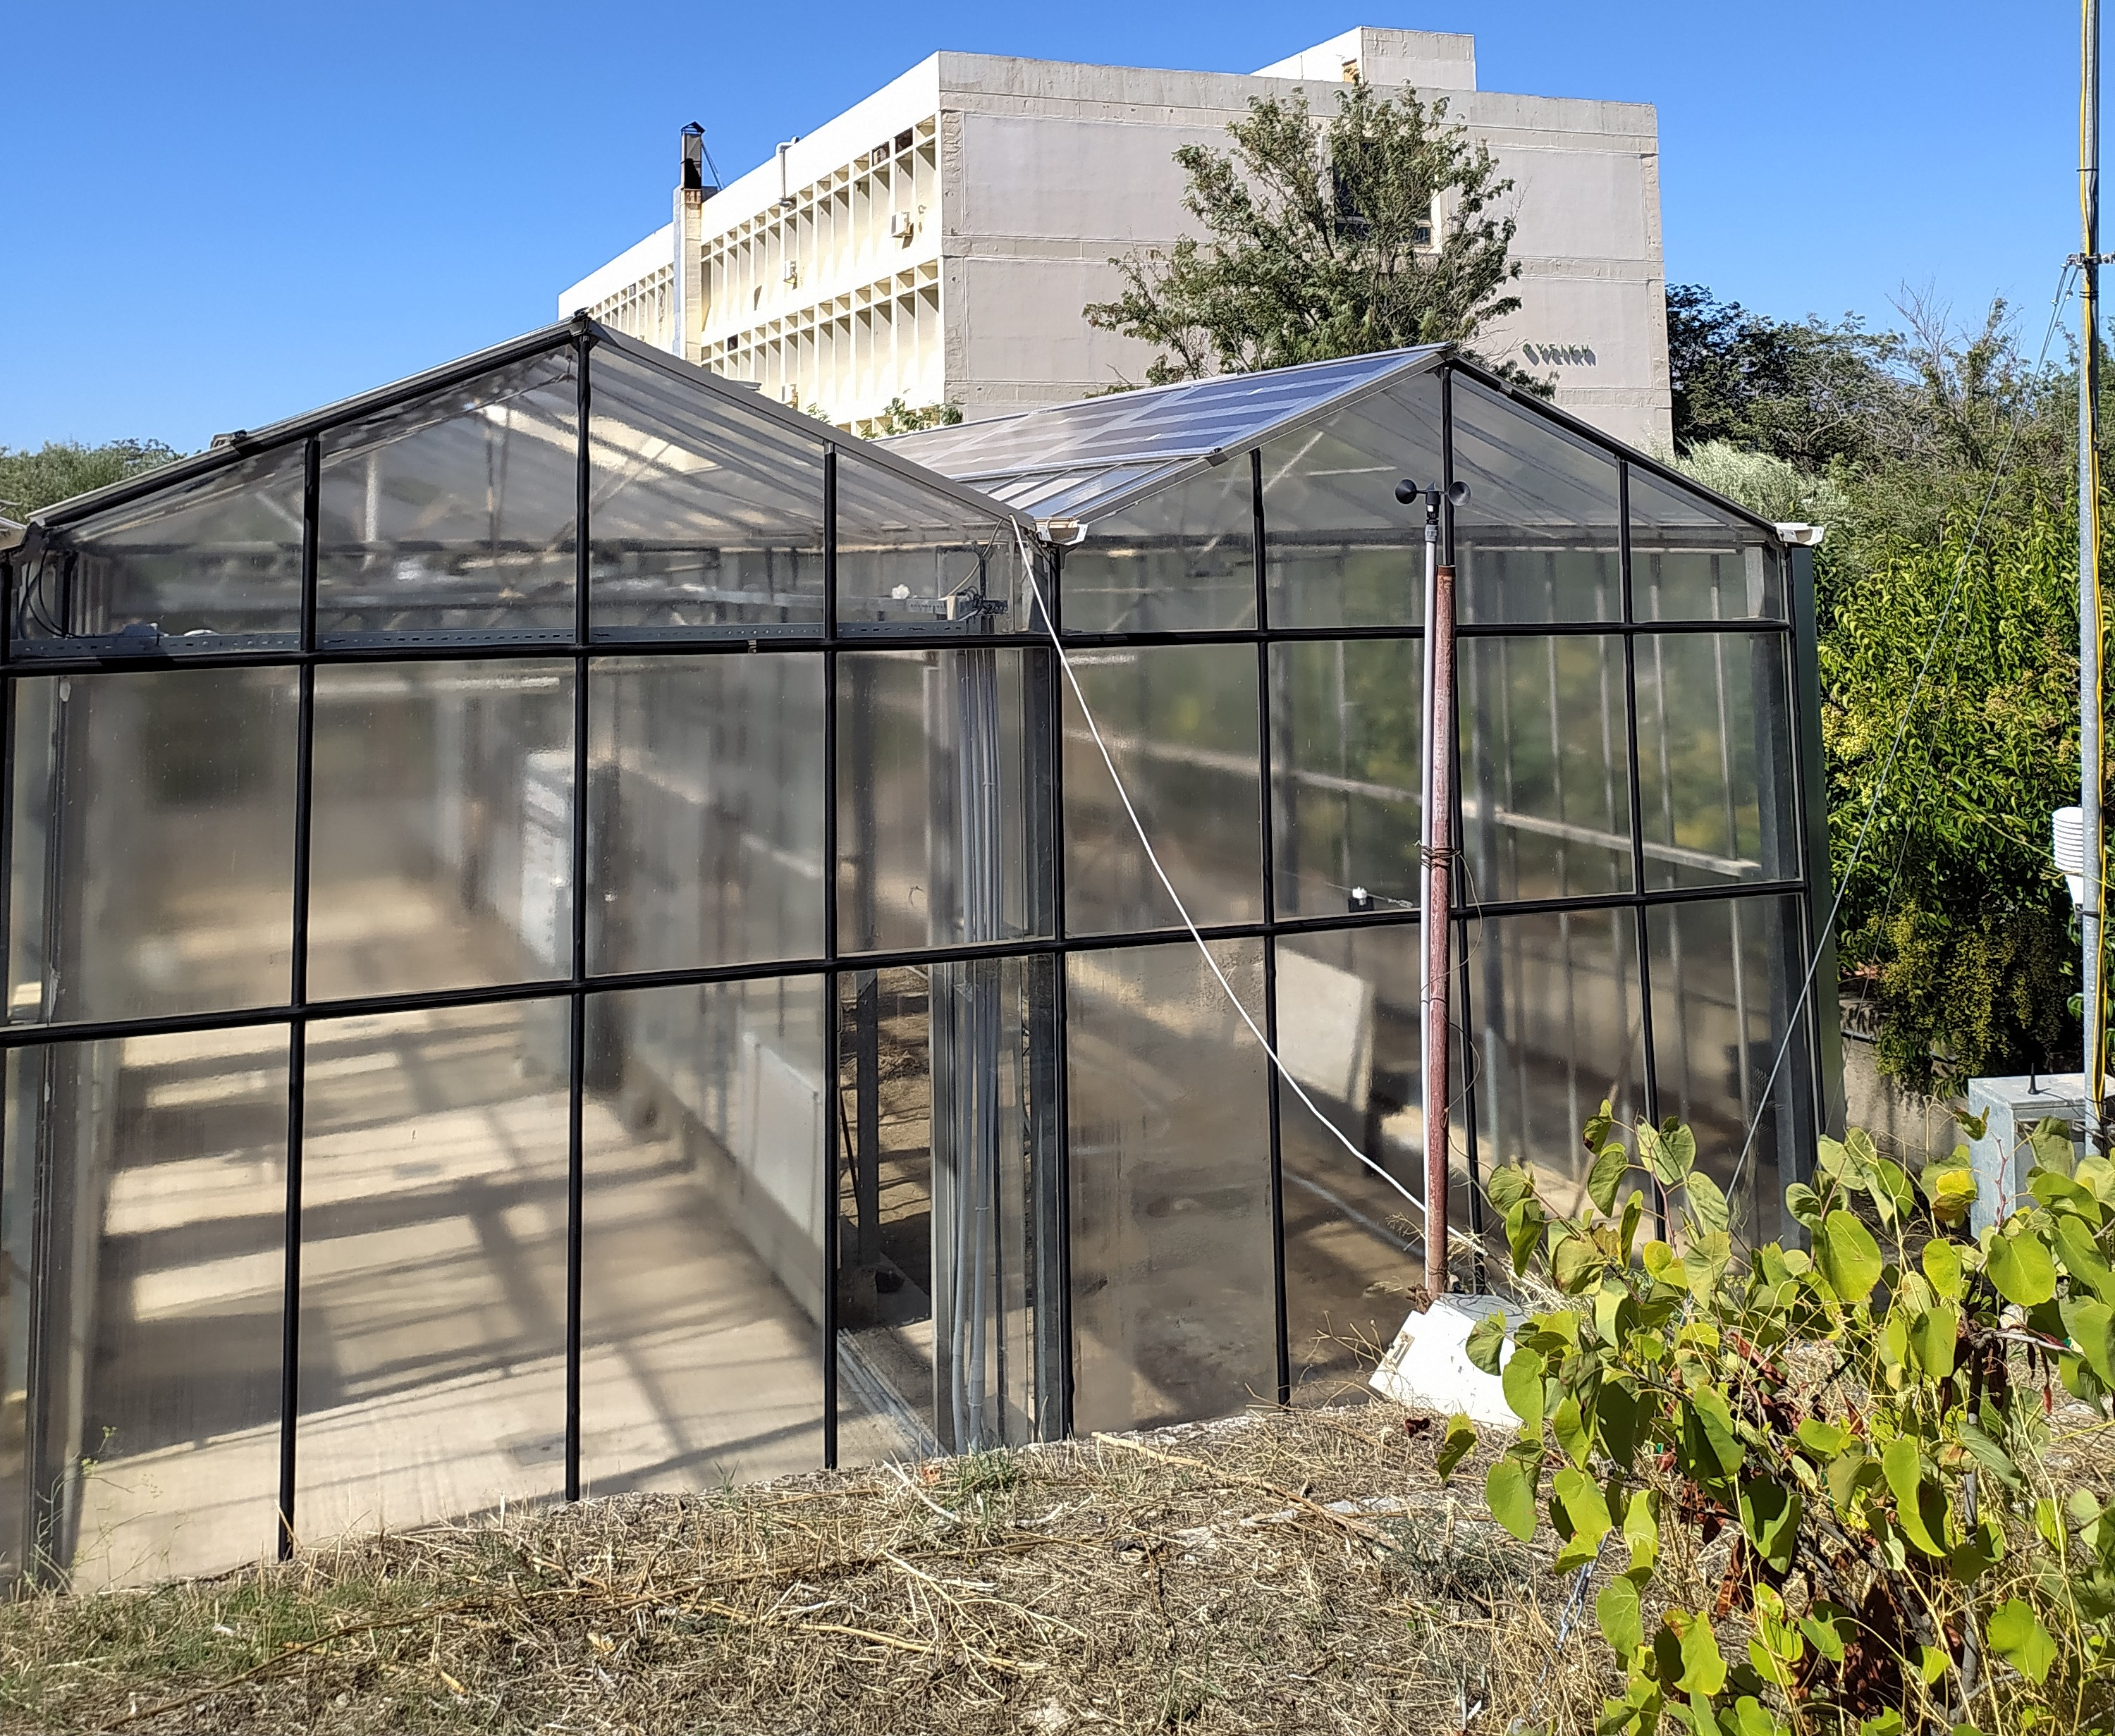
\includegraphics[width=0.8\textwidth]{Figures/Greenhouse.jpg}
    \caption{Βόρεια και Νότια Κατασκευαστική Μονάδα.}
    \label{fig_greenhouse_whole}
\end{figure}

%%%%%%%%%%%%%%%%%%%%%%%%%%%%%%%%%%%%%%%%%%
\subsection{Εξοπλισμός}\label{sub_eksoplismos}
Για την καταγραφή του μικροκλίματος του θερμοκηπίου στην υπό μελέτη μονάδα (Βόρεια Κατασκευαστική Μονάδας) γίνεται 
χρήση δύο συστημάτων λήψης δεδομένων, τα οποία είναι τοποθετημένα στο μέσον της μικρής πλευράς του θερμοκηπίου και σε 
σημεία που αντιστοιχούν στο \sfrac{1}{4} και \sfrac{3}{4} του μήκους του θερμοκηπίου. Τα συστήματα αυτά αποτελούνται από 
αισθητήρες \english{MP101A-T7-WAW} της εταιρείας \english{Rotronic} για την καταγραφή δεδομένων της θερμοκρασίας και της 
σχετικής υγρασίας, αισθητήρες (πυρανόμετρο) \english{CMP3} της εταιρείας \english{Kipp \& Zonen} για την καταγραφή 
δεδομένων της ολικής ηλιακής ακτινοβολίας σε οριζόντιο επίπεδο (\english{Global Horizontal Irradiance – GHI}) και αισθητήρες 
\english{ParLite} της εταιρείας \english{Kipp \& Zonen} για την καταγραφή δεδομένων της \english{PAR}. Εκτός του θερμοκηπίου και στην ανατολική πλευρά του είναι 
τοποθετημένος ένας αυτόματος μετεωρολογικός σταθμός (\english{Automatic Weather Station - AWS}) για την καταγραφή των 
εξωτερικών περιβαλλοντικών συνθηκών. Ο σταθμός αυτός έχει την δυνατότητα καταγραφής της θερμοκρασίας και της σχετικής 
υγρασίας με την χρήση του αισθητήρα \english{MP101A-T7-WAW}, της \english{GHI} με χρήση 
του αισθητήρα \english{CMP3}, της ταχύτητας του ανέμου με χρήση του αισθητήρα \english{A100K} της εταιρείας 
\english{Vector Instruments} τοποθετημένου σε ύψος \SI{6}{\meter} από την επιφάνεια του εδάφους και της θερμοκρασίας ουρανού 
με χρήση του αισθητήρα (πυργεόμετρο) \english{CGR3} της εταιρείας \english{Kipp \& Zonen}. Τόσο το πυρανόμετρο, όσο και το 
πυργεόμετρο του σταθμού βρίσκονται σε ύψος \SI{5}{\meter}. Τέλος, για την καταγραφή του ύψους βροχής είναι τοποθετημένο το 
βροχόμετρο 52203 της εταιρείας \english{R.M. Young}.

Τα καταγεγραμμένα από όλους τους αισθητήρες (εντός και εκτός θερμοκηπίου) μεταφέρονται ενσύρματα σε έναν 
\english{datalogger} (\english{CR1000} της εταιρείας \english{Campbell Scientific}). Τα δεδομένα λαμβάνονται είτε με 
χρονικό βήμα 10 λεπτών, είτε με χρονικό βήμα 1 λεπτού με τον συγκεκριμένο \english{datalogger} να έχει αποθηκευτική 
ικανότητα έως και 83 ημέρες. Οι αισθητήρες εντός και εκτός του θερμοκηπίου παρουσιάζονται στον Πίνακα \ref{tab_sensors}.

\begin{table}[ht]
    \centering
    \caption{Καταγεγραμμένες παράμετροι, αισθητήρες που χρησιμοποιήθηκαν για την καταγραφή τους και κατασκευαστές των 
    αισθητήρων.}\label{tab_sensors} 
   \begin{tabular}{>{\centering\arraybackslash}m{4.85cm} >{\centering\arraybackslash}m{4.85cm} >{\centering\arraybackslash}m{4.85cm}}
        \toprule
        \textbf{Παράμετρος} & \textbf{Αισθητήρας} & \textbf{Κατασκευαστής} \\
        \midrule
        \multicolumn{3}{c}{\textbf{Αυτόματος Μετεωρολογικός Σταθμός}} \\
        \midrule
        \english{Datalogger} &   \english{CR1000} & \english{Campbell Scientific} \\
        Θερμοκρασία \\ (\english{$T_{\text{$out$}}$}) & \english{MP101A-T7-WAW at 3m} & \english{Rotronic} \\
        Σχετική Υγρασία \\ (\english{$RH_{\text{$out$}}$}) & \english{MP101A-T7-WAW at 3m} & \english{Rotronic} \\
        Ταχύτητα Ανέμου \\ (\english{$WS$}) & \english{A100K at 6m} & \english{Vector Instruments} \\
        Ηλιακή Ακτινβολία \\ (\english{$GHI_{\text{$out$}}$}) & \english{CMP3 at 5m} & \english{Kipp \& Zonen} \\
        Βροχόπτωση \\ (\english{$R$}) & \english{52203} & \english{R.M. Young} \\
        Θερμοκρασία Ουρανού \\ (\english{$T_{\text{$sky$}}$}) & \english{CGR3 at 5m} & \english{Kipp \& Zonen} \\
        Υπέρυθρη Ακτινοβολία \\ (\english{$IR_{\text{$rad$}}$}) & \english{CGR3 at 5m} & \english{Kipp \& Zonen} \\
        \midrule
        \multicolumn{3}{c}{\textbf{Θερμοκήπιο}} \\
        \midrule
        Θερμοκρασία \\ (\english{$T_{\text{$in,1$}}$} \& \english{$T_{\text{$in,2$}}$}) & \english{MP101A-T7-WAW} & \english{Rotronic} \\
        Σχετική Υγρασία \\ (\english{$RH_{\text{$in,1$}}$} \& \english{$RH_{\text{$in,2$}}$}) & \english{CMP3} & \english{Rotronic} \\
        Ηλιακή Ακτινβολία \\ (\english{$GHI_{\text{$in,1$}}$} \& \english{$GHI_{\text{$in,2$}}$}) & \english{CMP3} & \english{Kipp \& Zonen} \\
        Φωτοσυνθετικά Ενεργή Ακτινοβολία \\ (\english{$PAR_{\text{$1$}}$} \& \english{$PAR_{\text{$2$}}$}) & \english{ParLite} & \english{Kipp \& Zonen} \\        
        \bottomrule
    \end{tabular}
\end{table}

\pagebreak

\noindent \textit{\textbf{\english{Datalogger “CR1000”}}}

\vspace{0.2cm}

O \english{datalogger CR1000} \lcitep{diataksi_bib1} είναι ένα σύστημα λήψης δεδομένων το 
οποίο έχει την δυνατότητα να υποστηρίξει αισθητήρες πολλών διαφορετικών τύπων, όπως αναλογι\-κούς (\english{analog}), 
παλμικούς (\english{pulse}), έξυπνους αισθητήρες (\english{smart sensors}) κ.ά. Για την λειτουργία του απαιτείται η 
παροχή τροφοδοσίας από 9,6 έως \SI{16}{\volt} \english{DC}, ενώ η μέση κατανάλωση ρεύματος για κατάσταση αδρανείας και 
για τροφοδοσία \SI{12}{\volt} \english{DC} είναι μικρότερη του \SI{1}{\milli\ampere}, γεγονός που τον καθιστά ιδανικό 
για απομακρυσμένους σταθμούς τροφοδοτούμενος από Φ/Β πάνελ. Σε ενεργό κατάσταση και για ρυθμό δειγματοληψίας με 
συχνότητα \SI{1}{\hertz}, η κατανάλωση ρεύματος είναι \SI{1}{\milli\ampere} για τροφοδοσία \SI{12}{\volt} \english{DC}, 
για ρυθμό δειγματοληψίας με συχνότητα \SI{100}{\hertz} χωρίς τον διακομιστή σειριακής διεπαφής 
(\english{Optical Isolated Interface}), \english{RS-232}, η κατανάλωση ρεύματος είναι \SI{16}{\milli\ampere}, ενώ για 
ρυθμό δειγματοληψίας με συχνότητα \SI{100}{\hertz} με τον διακομιστή σειριακής διεπαφής, η κατανάλωση ρεύματος είναι 
\SI{28}{\milli\ampere}. Διαθέτει 16 αναλογικές εισόδους μονού άκρου και 8 διαφορικές. Διαθέτει παράλληλα αποθηκευτική 
ικανότητα \SI{4}{\mega\byte} για διατήρηση των δεδομένων έως και 83 ημέρες με χρονικό βήμα λήψης 10 λεπτών. Το βασικό 
θερμοκρασιακό εύρος λειτουργίας του είναι μεταξύ -25 – \SI{50}{\degreeCelsius}, ενώ παρέχει την δυνατότητα ενσύρματης 
σύνδεσης σε δίκτυο με την προσθήκη μίας επιπλέον συσκευής. Στην συγκεκριμένη περίπτωση έχει χρησιμοποιηθεί η 
\english{NL115} της εταιρείας \english{Campbell Scientific}.

Επιπλέον, στον Αυτόματο Μετεωρολογικό Σταθμό υπάρχει εγκατεστημένος ένας πολυπλέκτης 16/32 καναλιών (ΑΜ16/32A της 
εταιρείας \english{Campbell Scientific}) και ένας διακομιστής σειριακής διεπαφής \english{RS-232} (\english{SC32A} της 
εταιρείας \english{Campbell Scientific}) για την άμεση επικοινωνία μεταξύ του \english{datalogger} και της σειριακής 
θύρας του υπολογιστή (Εικόνα \ref{fig_datalogger}).

Παρακάτω παρουσιάζονται πιο αναλυτικά τα τεχνικά χαρακτηριστικά των αισθητήρων που χρησιμοποιήθηκαν στην συγκεκριμένη 
εργασία.

\begin{figure}[ht]%
    \centering
    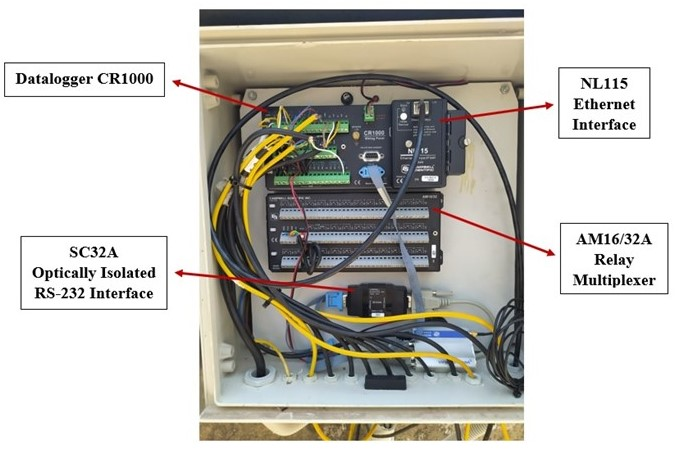
\includegraphics[width=0.8\textwidth]{Figures/datalogger.jpg}
    \caption{\english{Datalogger CR1000}, διαkομιστής σειριαkής διεπαφής \english{RS-232}, διεπαφή \english{Ethernet NL115} και πολυπλέkτης ΑΜ16/32Α.}
    \label{fig_datalogger}
\end{figure}

\noindent \textit{\textbf{Αισθητήρας θερμοκρασίας – σχετικής υγρασίας \english{“MP101A-T7-WAW”}}}

\vspace{0.2cm}

Ο αισθητήρας \english{MP101A-T7-WAW} \lcitep{diataksi_bib2} ενσωματώνει δύο διαφορετικούς 
αισθητήρες, από την μία τον \english{PT100 1/3 DIN Class B} για την μέτρηση της θερμοκρασίας με δυνατότητα καταγραφής 
(\english{operating range}) σε εύρος από -40 – \SI{85}{\degreeCelsius} με ακρίβεια στους 23 $\pm$ \SI{5}{\degreeCelsius}, 
$\pm$\SI{0.3}{\kelvin}. Από την άλλη, για την μέτρηση της σχετικής υγρασίας, τον \english{Hygromer IN-1}, με δυνατότητα 
καταγραφής σε εύρος 0 – \SI{100}{\percent} με ακρίβεια στους 23 $\pm$ \SI{5}{\degreeCelsius}, $\pm$\SI{1,5}{\percent}. 
Η μακροπρόθεσμη σταθερότητα (\english{long-term stability}) για την υγρασία υπό κανονικές συνθήκες του αισθητήρα είναι 
μικρότερη από \SI{1}{\percent} ανά έτος. Τέλος, η μέγιστη κατανάλωση ρεύματος ανέρχεται στα \SI{8}{\milli\ampere} για 
τροφοδοσία 4,8 – \SI{30}{\volt} \english{DC} ή \SI{7}{\milli\ampere} για τροφοδοσία 3,6 έως \SI{12}{\volt} \english{DC}, 
ενώ ο χρόνος απόκρισης του αισθητήρα είναι μικρότερος από 15 \english{sec}. Στην Εικόνα \ref{fig_temp_meter}α παρουσιάζεται 
ο αισθητήρας \english{MP101A-T7-WAW} εντός του θερμοκηπίου, ενώ στην Εικόνα \ref{fig_temp_meter}β, στον Αυτόματο 
Μετεωρολογικό Σταθμό καλυπτόμενος από ένα φυσικώς αεριζόμενο κάλυμμα.

\begin{figure}[ht]
    \centering
    \begin{subfigure}{0.5\textwidth}
        \centering
        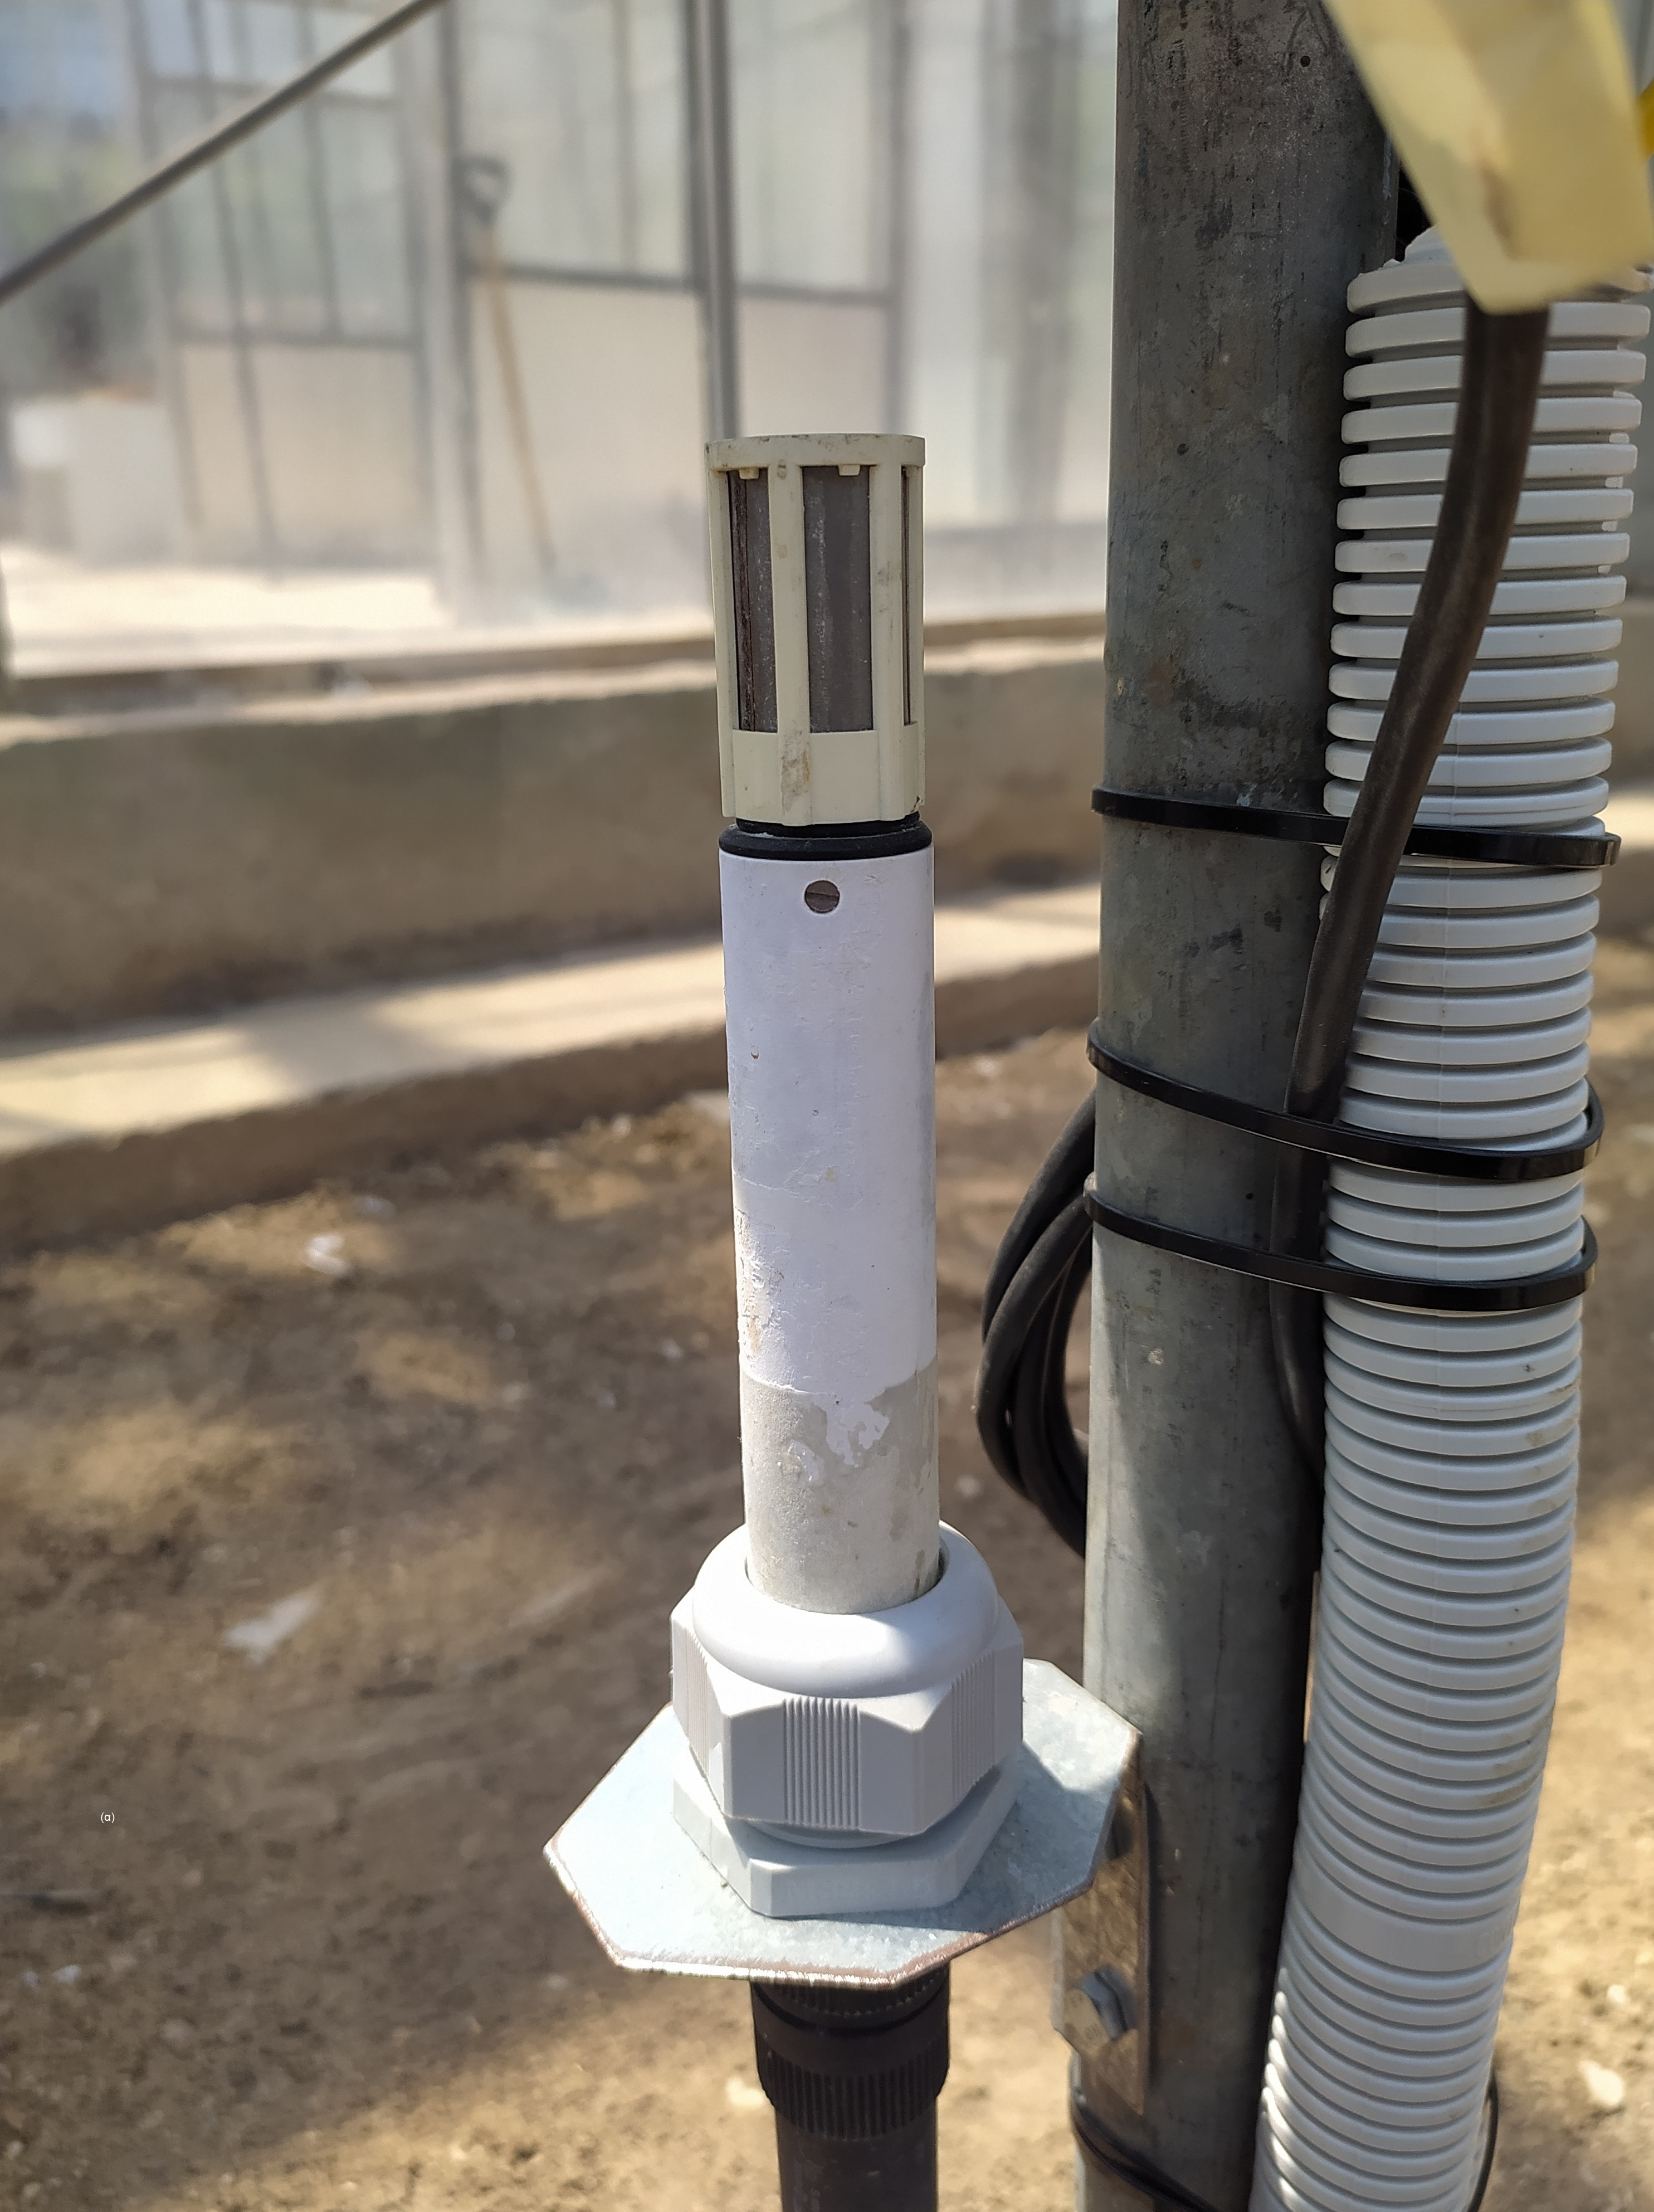
\includegraphics[width=0.8\linewidth, height=83mm]{Figures/temp_meter_in.jpg}
        \caption*{(α)}{}
    \end{subfigure}%
    \begin{subfigure}{0.5\textwidth}
        \centering
        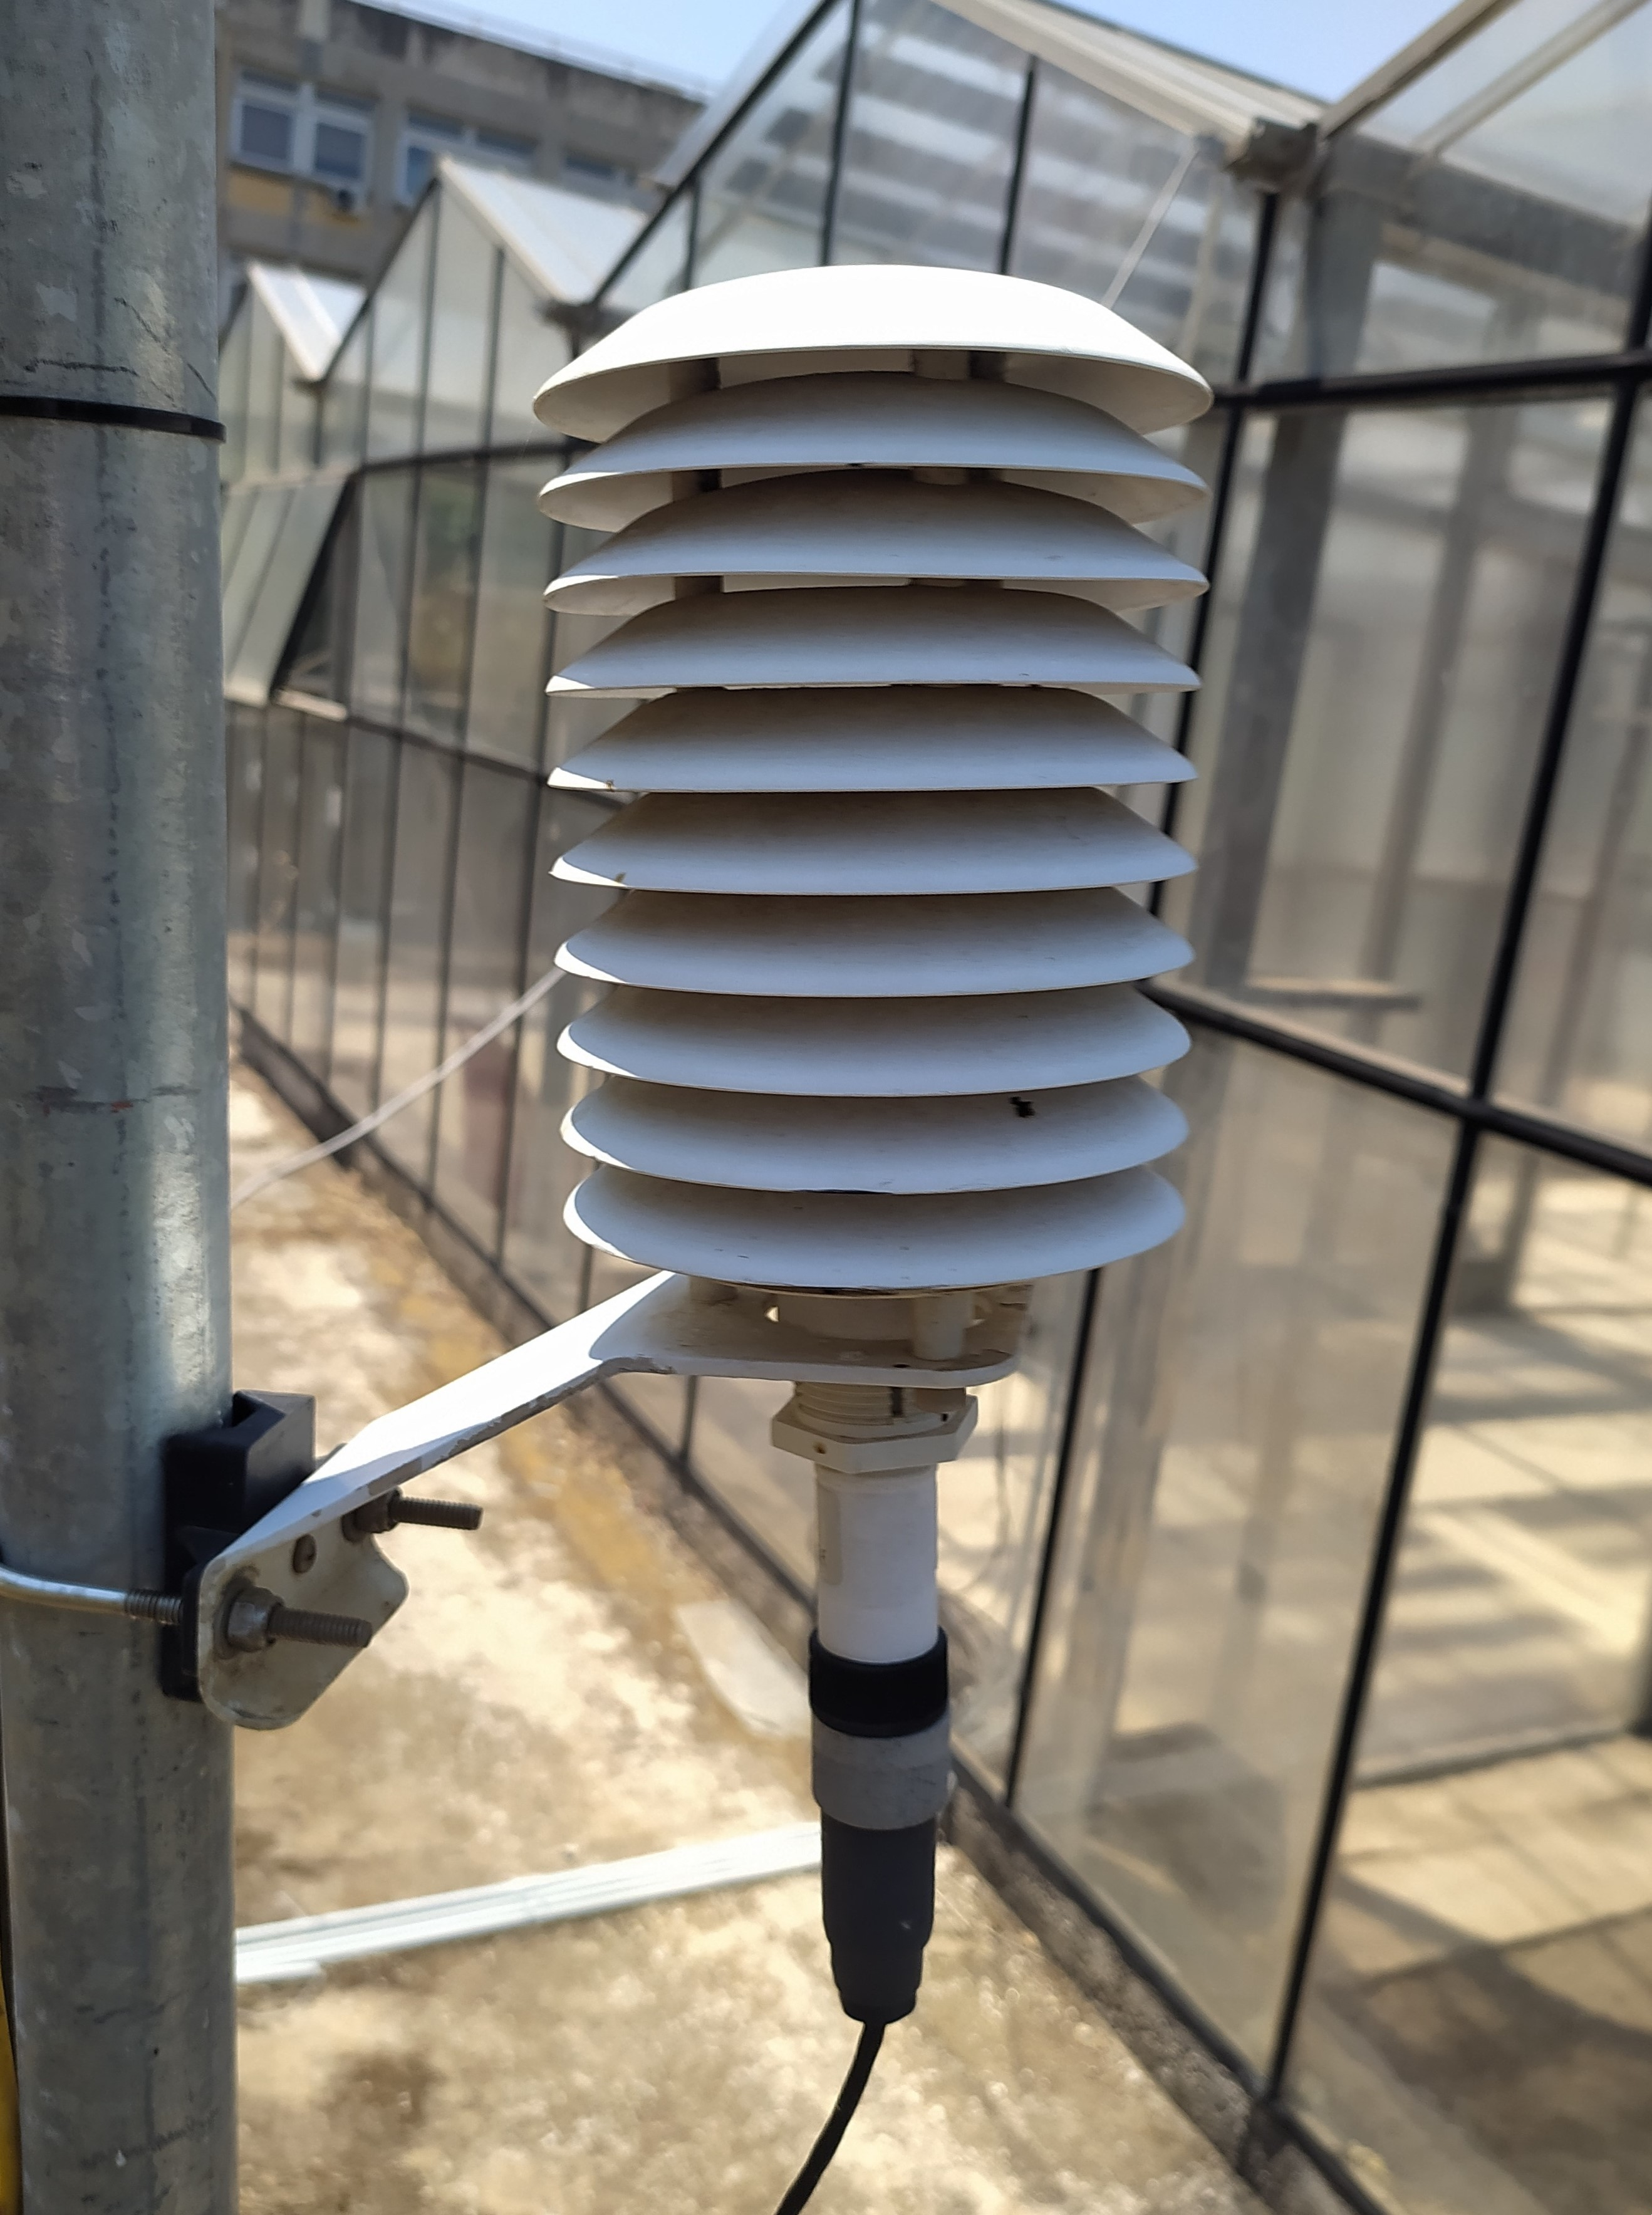
\includegraphics[width=0.8\linewidth, height=83mm]{Figures/temp_meter_out.jpg}
        \caption*{(β)}{}
    \end{subfigure}%
    \caption{Aισθητήρας \english{MP101A-T7-WAW} (α) εντός του θερμοκηπίου (β) εκτός του θερμοκηπίου.}
    \label{fig_temp_meter}
\end{figure}

\pagebreak

\noindent \textit{\textbf{Πυρανόμετρο \english{CMP3}}}

\vspace{0.2cm}

Το πυρανόμετρο \english{CMP3} \lcitep{diataksi_bib3} (Εικόνα \ref{fig_pyranometer_in}) είναι ένας 
παθητικός αισθητήρας με μηδενική, δηλαδή, κατανάλωση ρεύματος. Το εύρος του ηλιακού φάσματος (\english{spectral range}) 
που μπορεί να καλύψει είναι από 300 – \SI{800}{\nano\meter}, ενώ η ευαισθησία (\english{sensitivity}) του οργάνου είναι 
μεταξύ 10 και \SI{32}{\micro\volt\per\watt\per\meter\squared}, με χρόνο απόκρισης μικρότερο των 20 \english{sec}. Το 
σφάλμα μη γραμμικότητας (\english{non-linearity}) για την μεταβολή της ευαισθησίας σε εύρος ηλιακής ακτινοβολίας 0 – 
\SI{1000}{\watt\per\meter\squared} είναι μικρότερο του \SI{2}{\percent}. Παράλληλα, η εξάρτηση της ευαισθησίας του οργάνου 
από την θερμοκρασία σε ένα εύρος -10 – \SI{40}{\degreeCelsius} είναι μικρότερη του \SI{4}{\percent}. Η απόκριση 
κατευθυντικότητας (\english{directional response}) του \english{CMP3} για ακτινοβολία δέσμης 
\SI{1000}{\watt\per\meter\squared} για γωνία μεγαλύτερη των \SI{80}{\degree} είναι μικρότερη από 
\SI{20}{\watt\per\meter\squared}. Τέλος, το σφάλμα κλίσης (\english{tilt error}) στα \SI{1000}{\watt\per\meter\squared} 
είναι μικρότερο του \SI{1,5}{\percent}, η μη σταθερότητά του είναι μικρότερη του \SI{1}{\percent} ανά έτος, η αβεβαιότητα 
στο ημερήσιο άθροισμα είναι μικρότερη του \SI{10}{\percent}, ενώ το εύρος θέασης (\english{field view}) είναι 
\SI{180}{\degree}.

Η σχέση βάσει της οποίας υπολογίζεται η ακτινοβολία μέσω του οργάνου είναι:
\begin{equation}
    E_{\english{solar}} = \frac{U_{\english{emf}}}{S}
    \label{eq_E_solar}
\end{equation}

\noindent όπου \english{$E_{\text{$solar$}}$}, η ακτινοβολία (\english{irradiance}) σε \SI{}{\watt\per\meter\squared}, 
\english{$U_{\text{$emf$}}$}, η τάση εξόδου (\english{output voltage}) σε \SI{}{\milli\volt} και $S$ η ευαισθησία 
(\english{sensitivity}) σε \SI{}{\milli\volt\per\watt\per\meter\squared}. 

\begin{figure}[ht]%
    \centering
    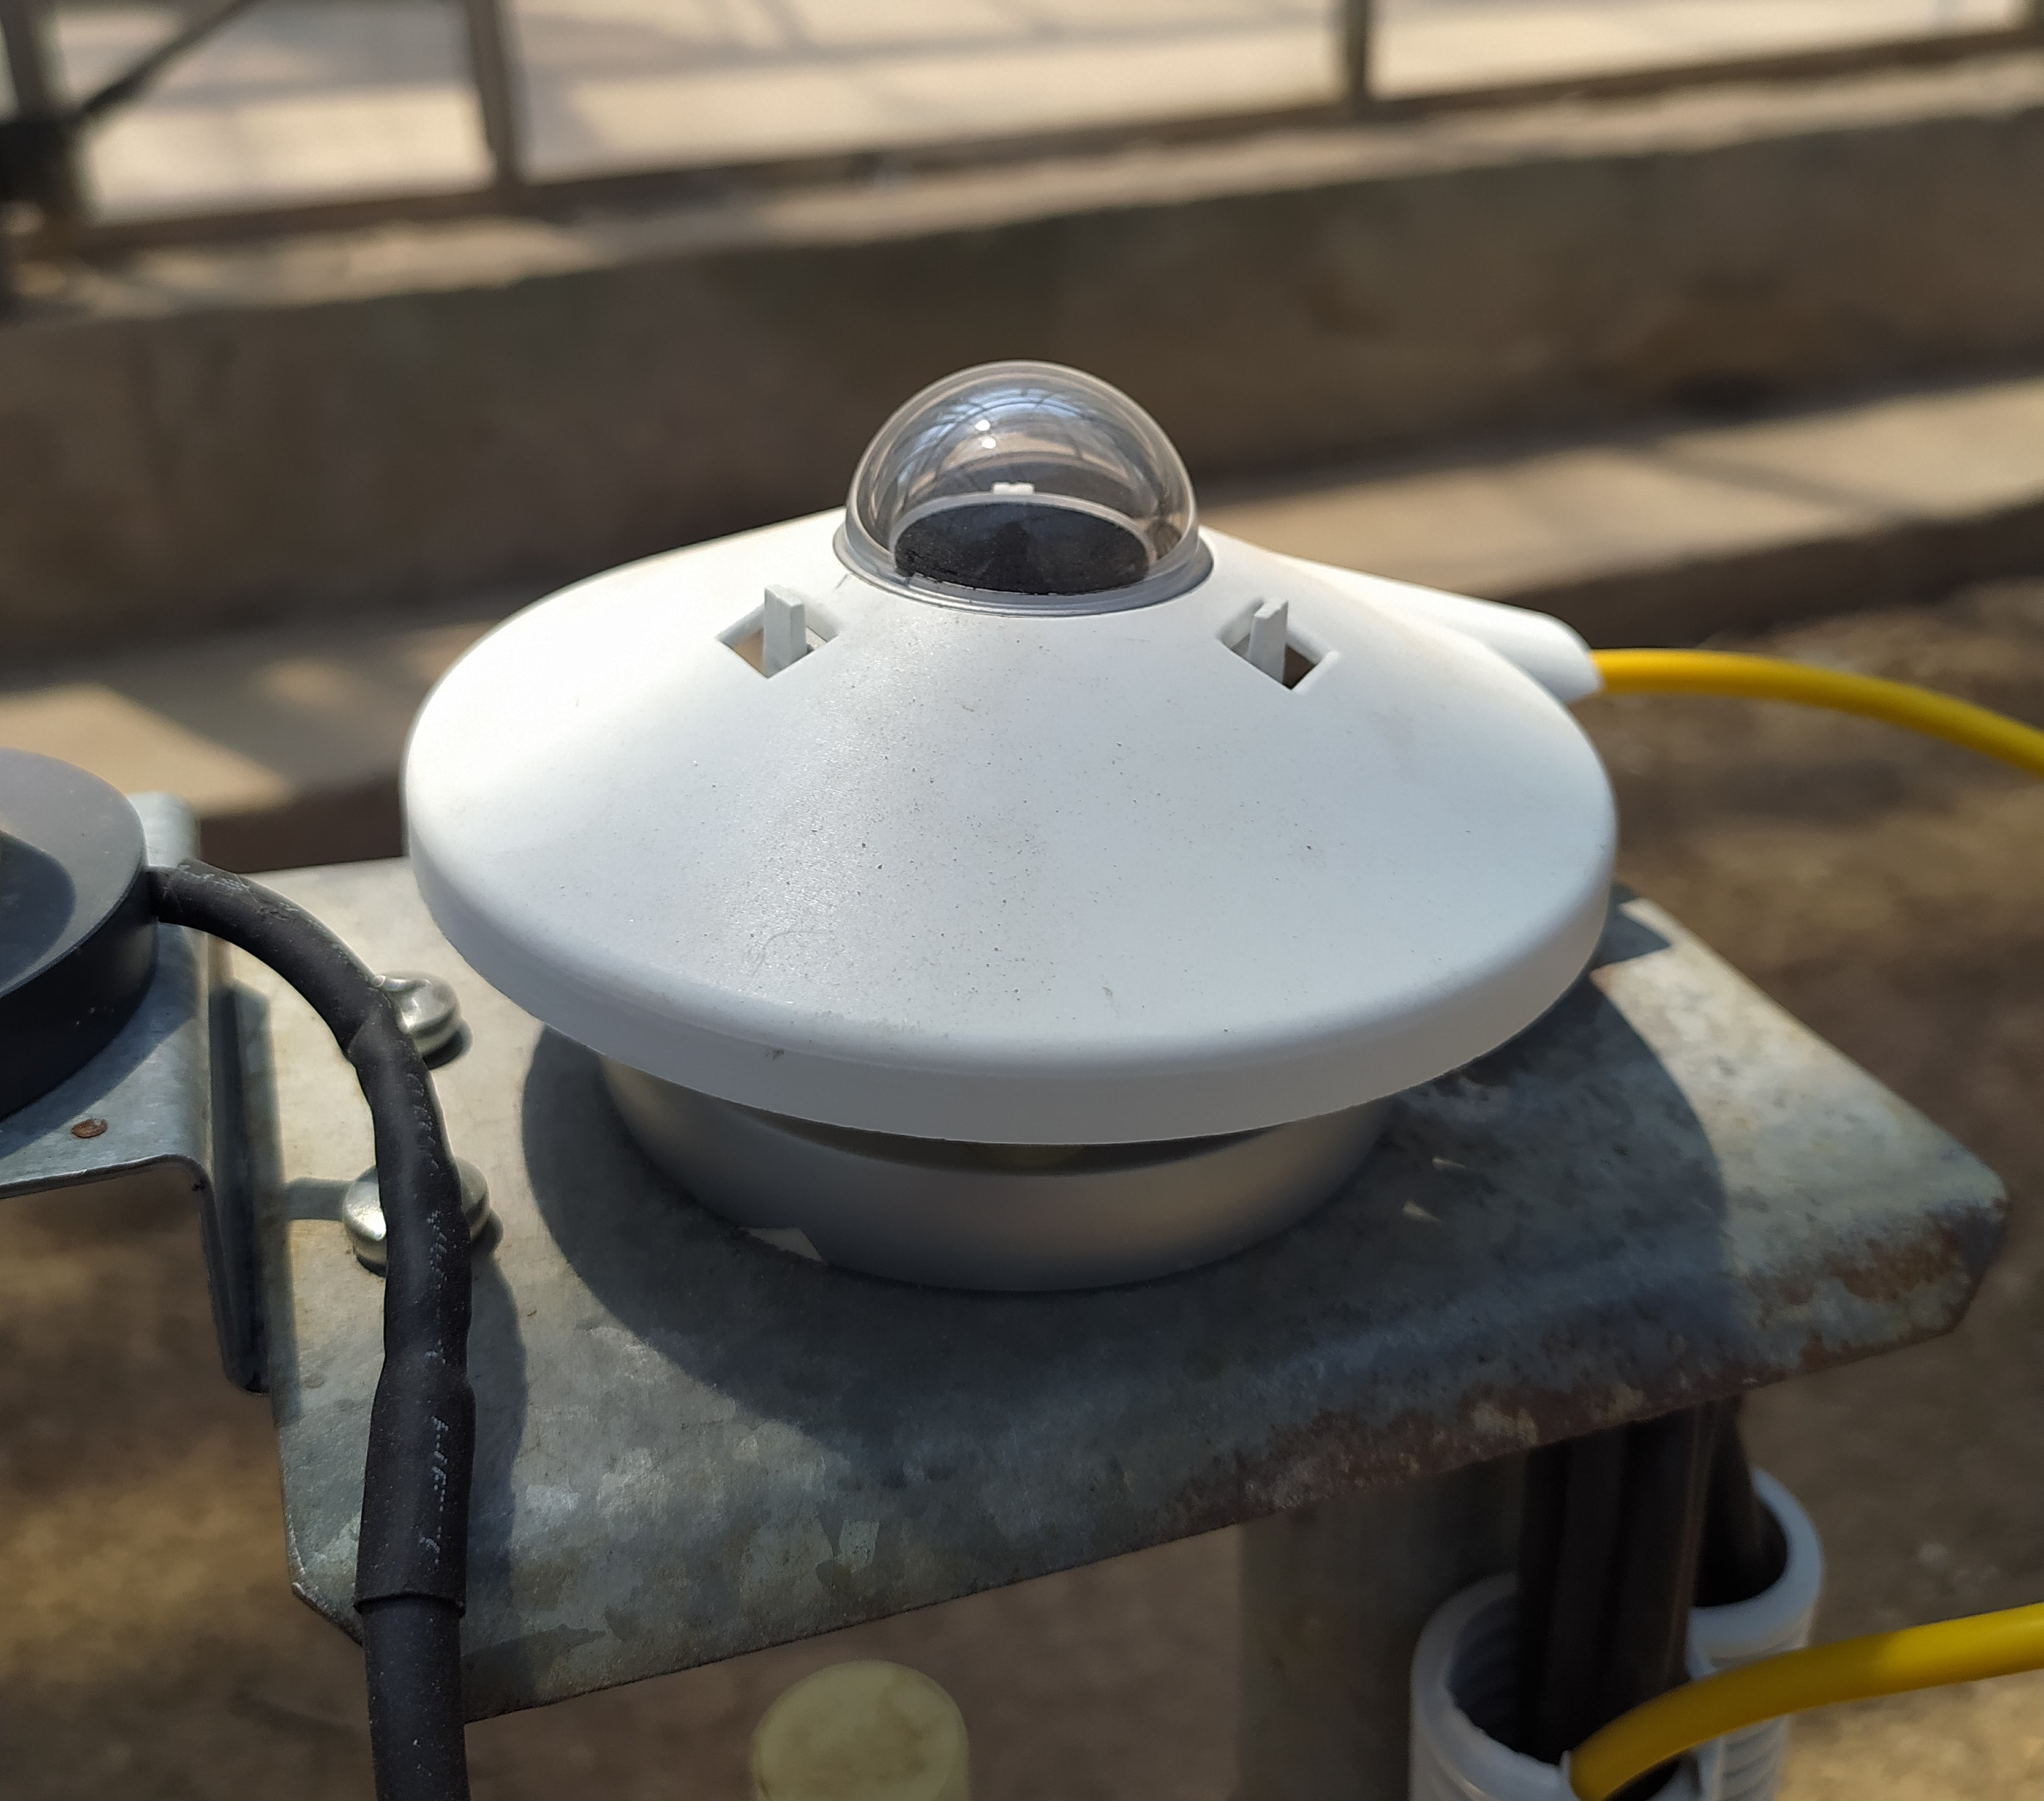
\includegraphics[scale=0.08]{Figures/pyranometer.jpg}
    \caption{Πυρανόμετρο \english{CMP3} εντός του θερμοκηπίου.}
    \label{fig_pyranometer_in}
\end{figure}

\pagebreak

\noindent \textit{\textbf{Ανεμόμετρο \english{“A100K”}}}

\vspace{0.2cm}

Όπως και ο αισθητήρας θερμοκρασίας – σχετικής υγρασίας, έτσι και το ανεμόμετρο \english{A100K} \lcitep{diataksi_bib4} 
(Εικόνα \ref{fig_anemometer}) απαιτεί μία τάση τροφοδοσίας 10 – \SI{30}{\volt} \english{DC}, ενώ το ρεύμα τροφοδοσίας 
είναι \SI{30}{\milli\ampere} στα \SI{12}{\volt}. Το εύρος θερμοκρασιών λειτουργίας είναι -50 – \SI{70}{\degreeCelsius}. 
Από πλευράς επιδόσεων, το ανεμόμετρο \english{A100K} έχει την δυνατότητα μέτρησης ταχυτήτων σε εύρος 0 – 
\SI{75}{\meter\per\second}, ενώ η ελάχιστη τιμή της ταχύτητας του ανέμου που απαιτείται για την λειτουργία του 
(\english{threshold}) είναι \SI{0.15}{\meter\per\second}. Όσον αφορά την ακρίβεια του οργάνου αυτή παρουσιάζει σφάλμα 
\SI{1}{\percent} για ταχύτητες μεταξύ 10 και \SI{55}{\meter\per\second}, \SI{2}{\percent} για ταχύτητες μεγαλύτερες των 
\SI{55}{\meter\per\second} και \SI{0,1}{\percent} για ταχύτητες μεταξύ 0,1 και \SI{10}{\meter\per\second}.

\begin{figure}[ht]%
    \centering
    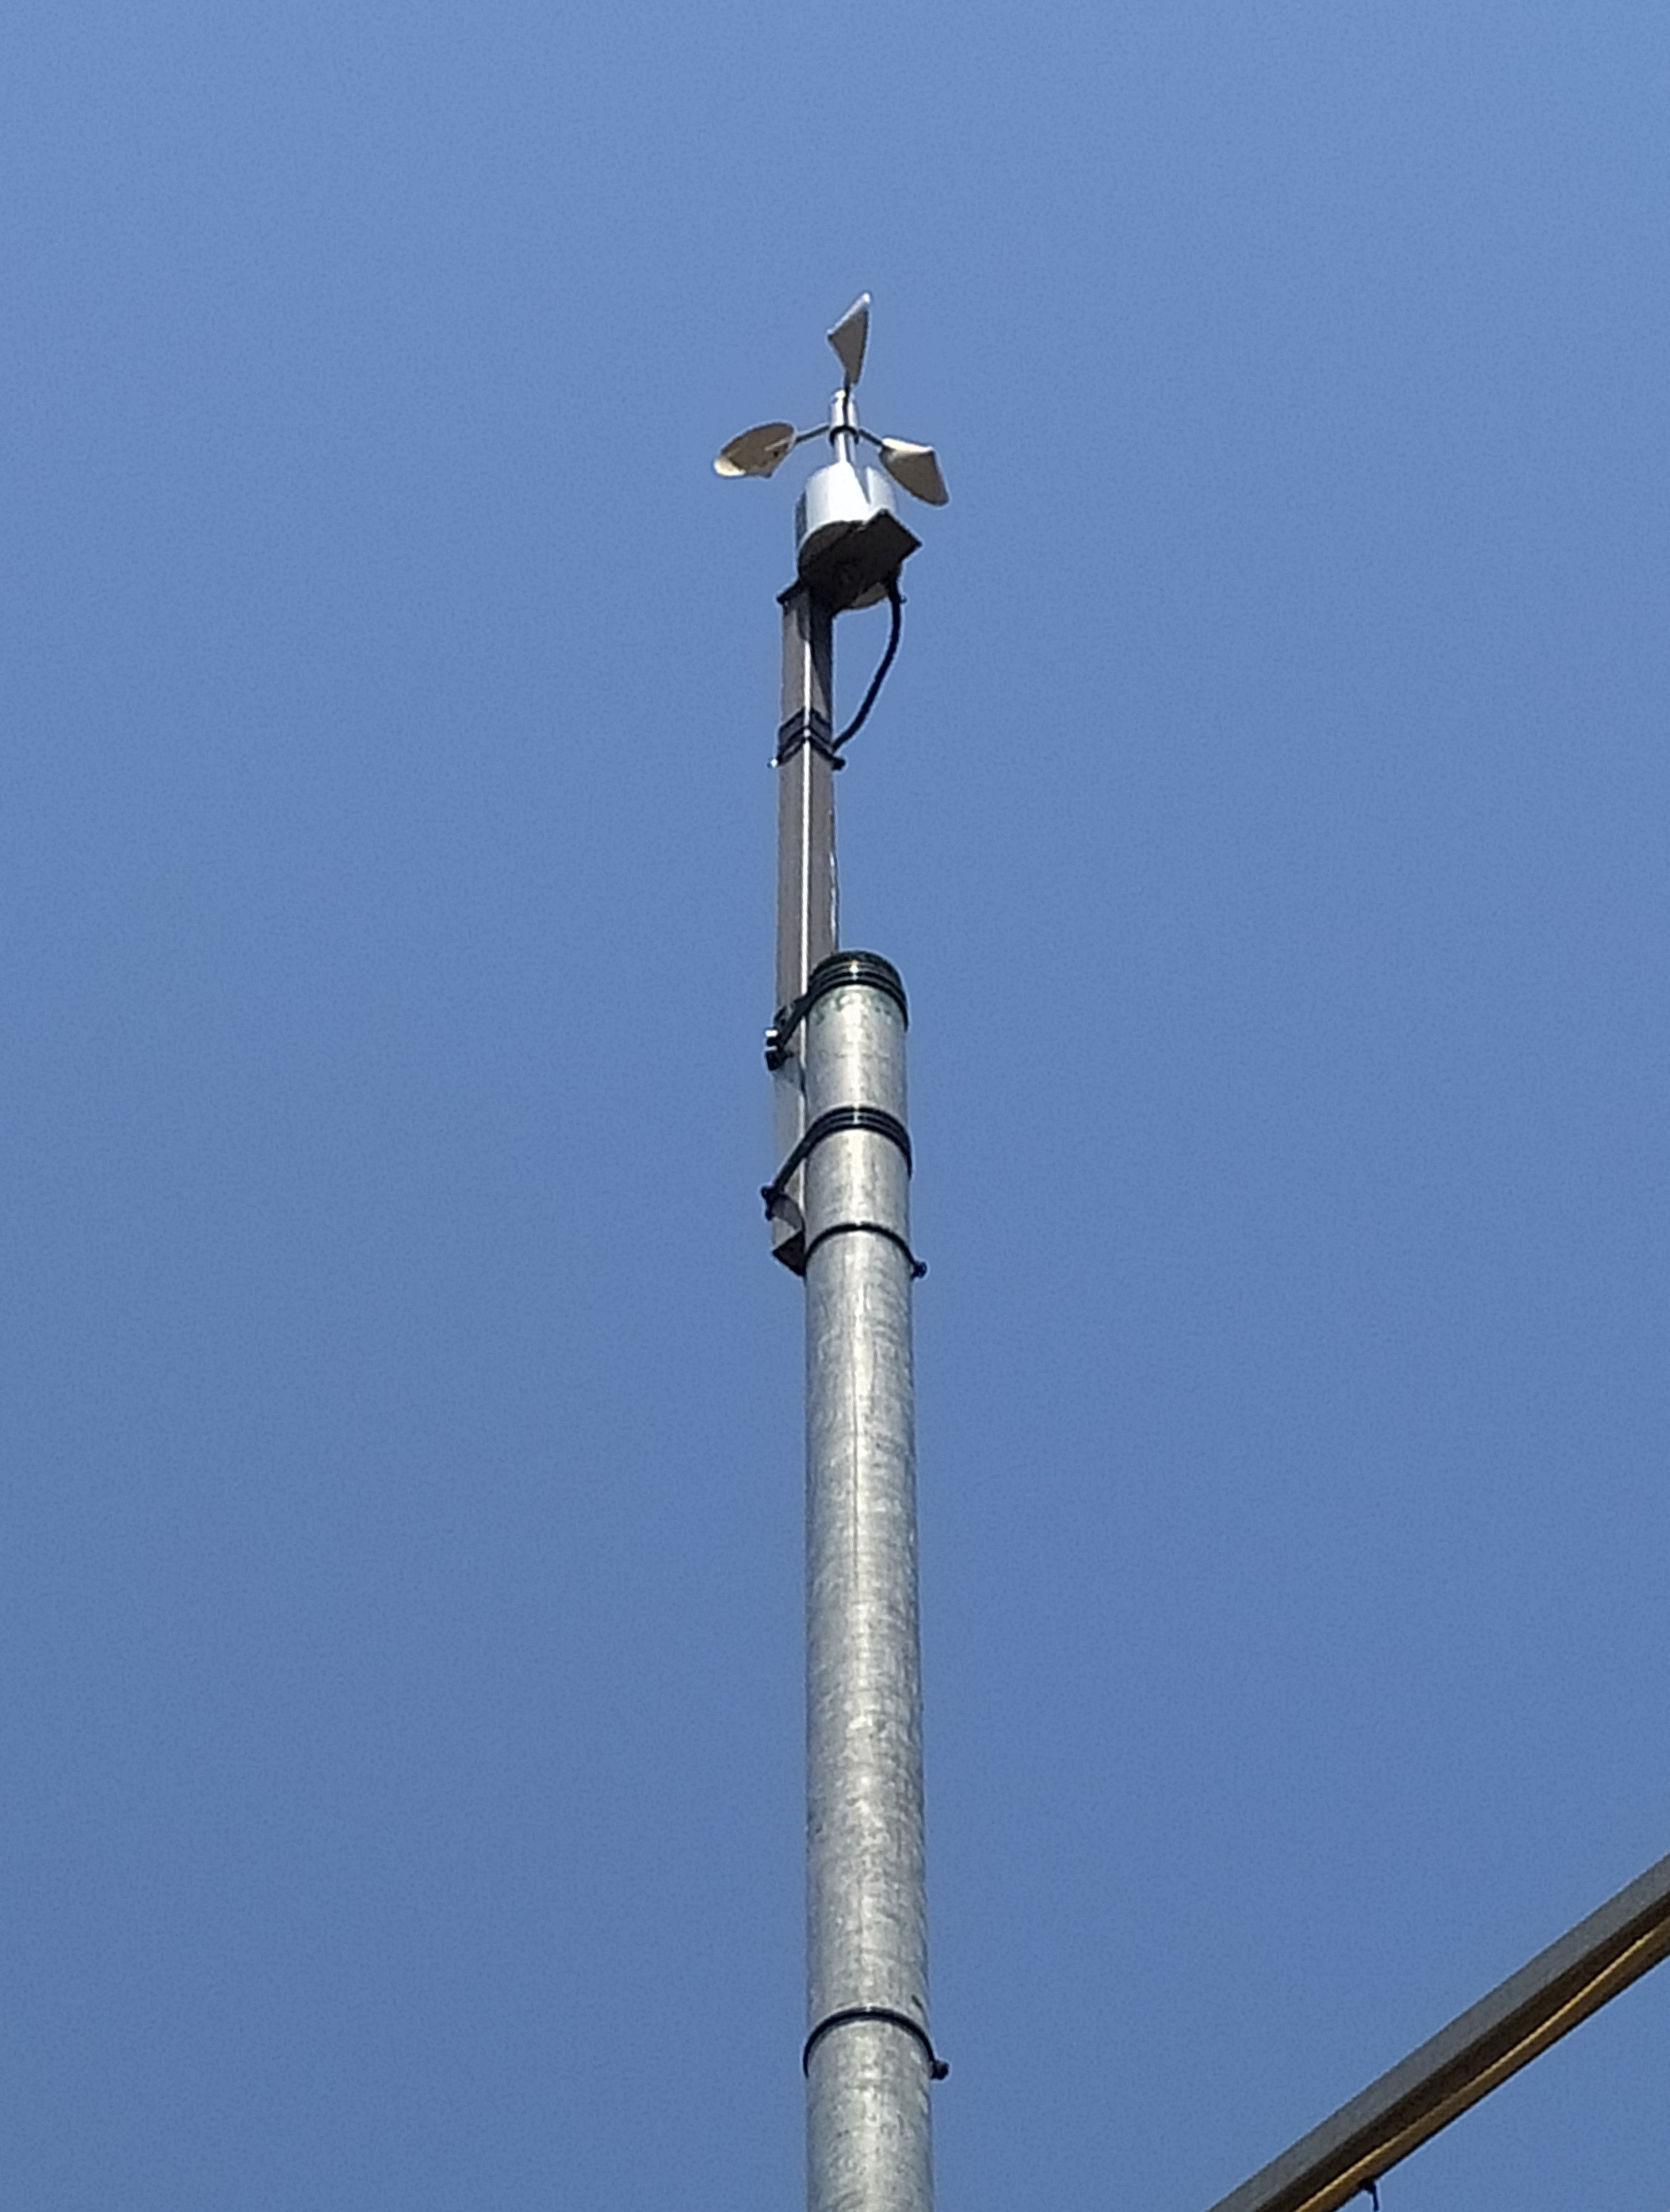
\includegraphics[scale=0.08]{Figures/anemometer.jpg}
    \caption{Ανεμόμετρο \english{A100K}.}
    \label{fig_anemometer}
\end{figure}

\vspace{0.4cm}

\noindent \textit{\textbf{Αισθητήρας φωτοσυνθετικά ενεργής ακτινοβολίας \english{“ParLite”}}}

\vspace{0.2cm}

Ο αισθητήρας \english{ParLite} \lcitep{diataksi_bib5} (Εικόνα \ref{fig_parlite}) είναι επίσης ένας παθητικός 
αισθητήρας με μηδενική κατανάλωση ρεύματος. Το εύρος του ηλιακού φάσματος που καλύπτει είναι από 400 – 
\SI{700}{\nano\meter}, το εύρος δηλαδή των μηκών κύματος που αντιστοιχεί στην \english{PAR}. Η αντί\-σταση 
του οργάνου είναι \SI{240}{\ohm}, ενώ η ευαισθησία του είναι 
\SI{4,89}{\micro\volt\per\micro\mol\per\second\per\meter\squared}, με χρόνο απόκρισης μικρότερο του 0,1 \english{sec}. 
Η εξάρτηση της ευαισθησίας του οργάνου από την θερμοκρασία είναι στα πλαίσια του $\sim$\SI{0,2}{\percent} ανά 
\SI{}{\degreeCelsius}, η μη σταθερότητά του είναι στα πλαίσια του $\sim$\SI{2}{\percent} ανά έτος, το σφάλμα μη 
γραμμικότητας για ακτινοβολία μεγαλύτερη των \SI{10000}{\micro\mol\per\second\per\meter\squared} είναι στα πλαίσια 
του $\sim$\SI{1}{\percent}, ενώ το σφάλμα για προσπίπτουσα ακτινοβολία μεγαλύτερη των \SI{80}{\degree} είναι περίπου 
\SI{10}{\percent}. Τέλος, το εύρος των θερμοκρασιών λειτουργίας είναι -30 – \SI{70}{\degreeCelsius}, ενώ της σχετικής 
υγρασίας είναι 0 – \SI{100}{\percent}.

\begin{figure}[ht]%
    \centering
    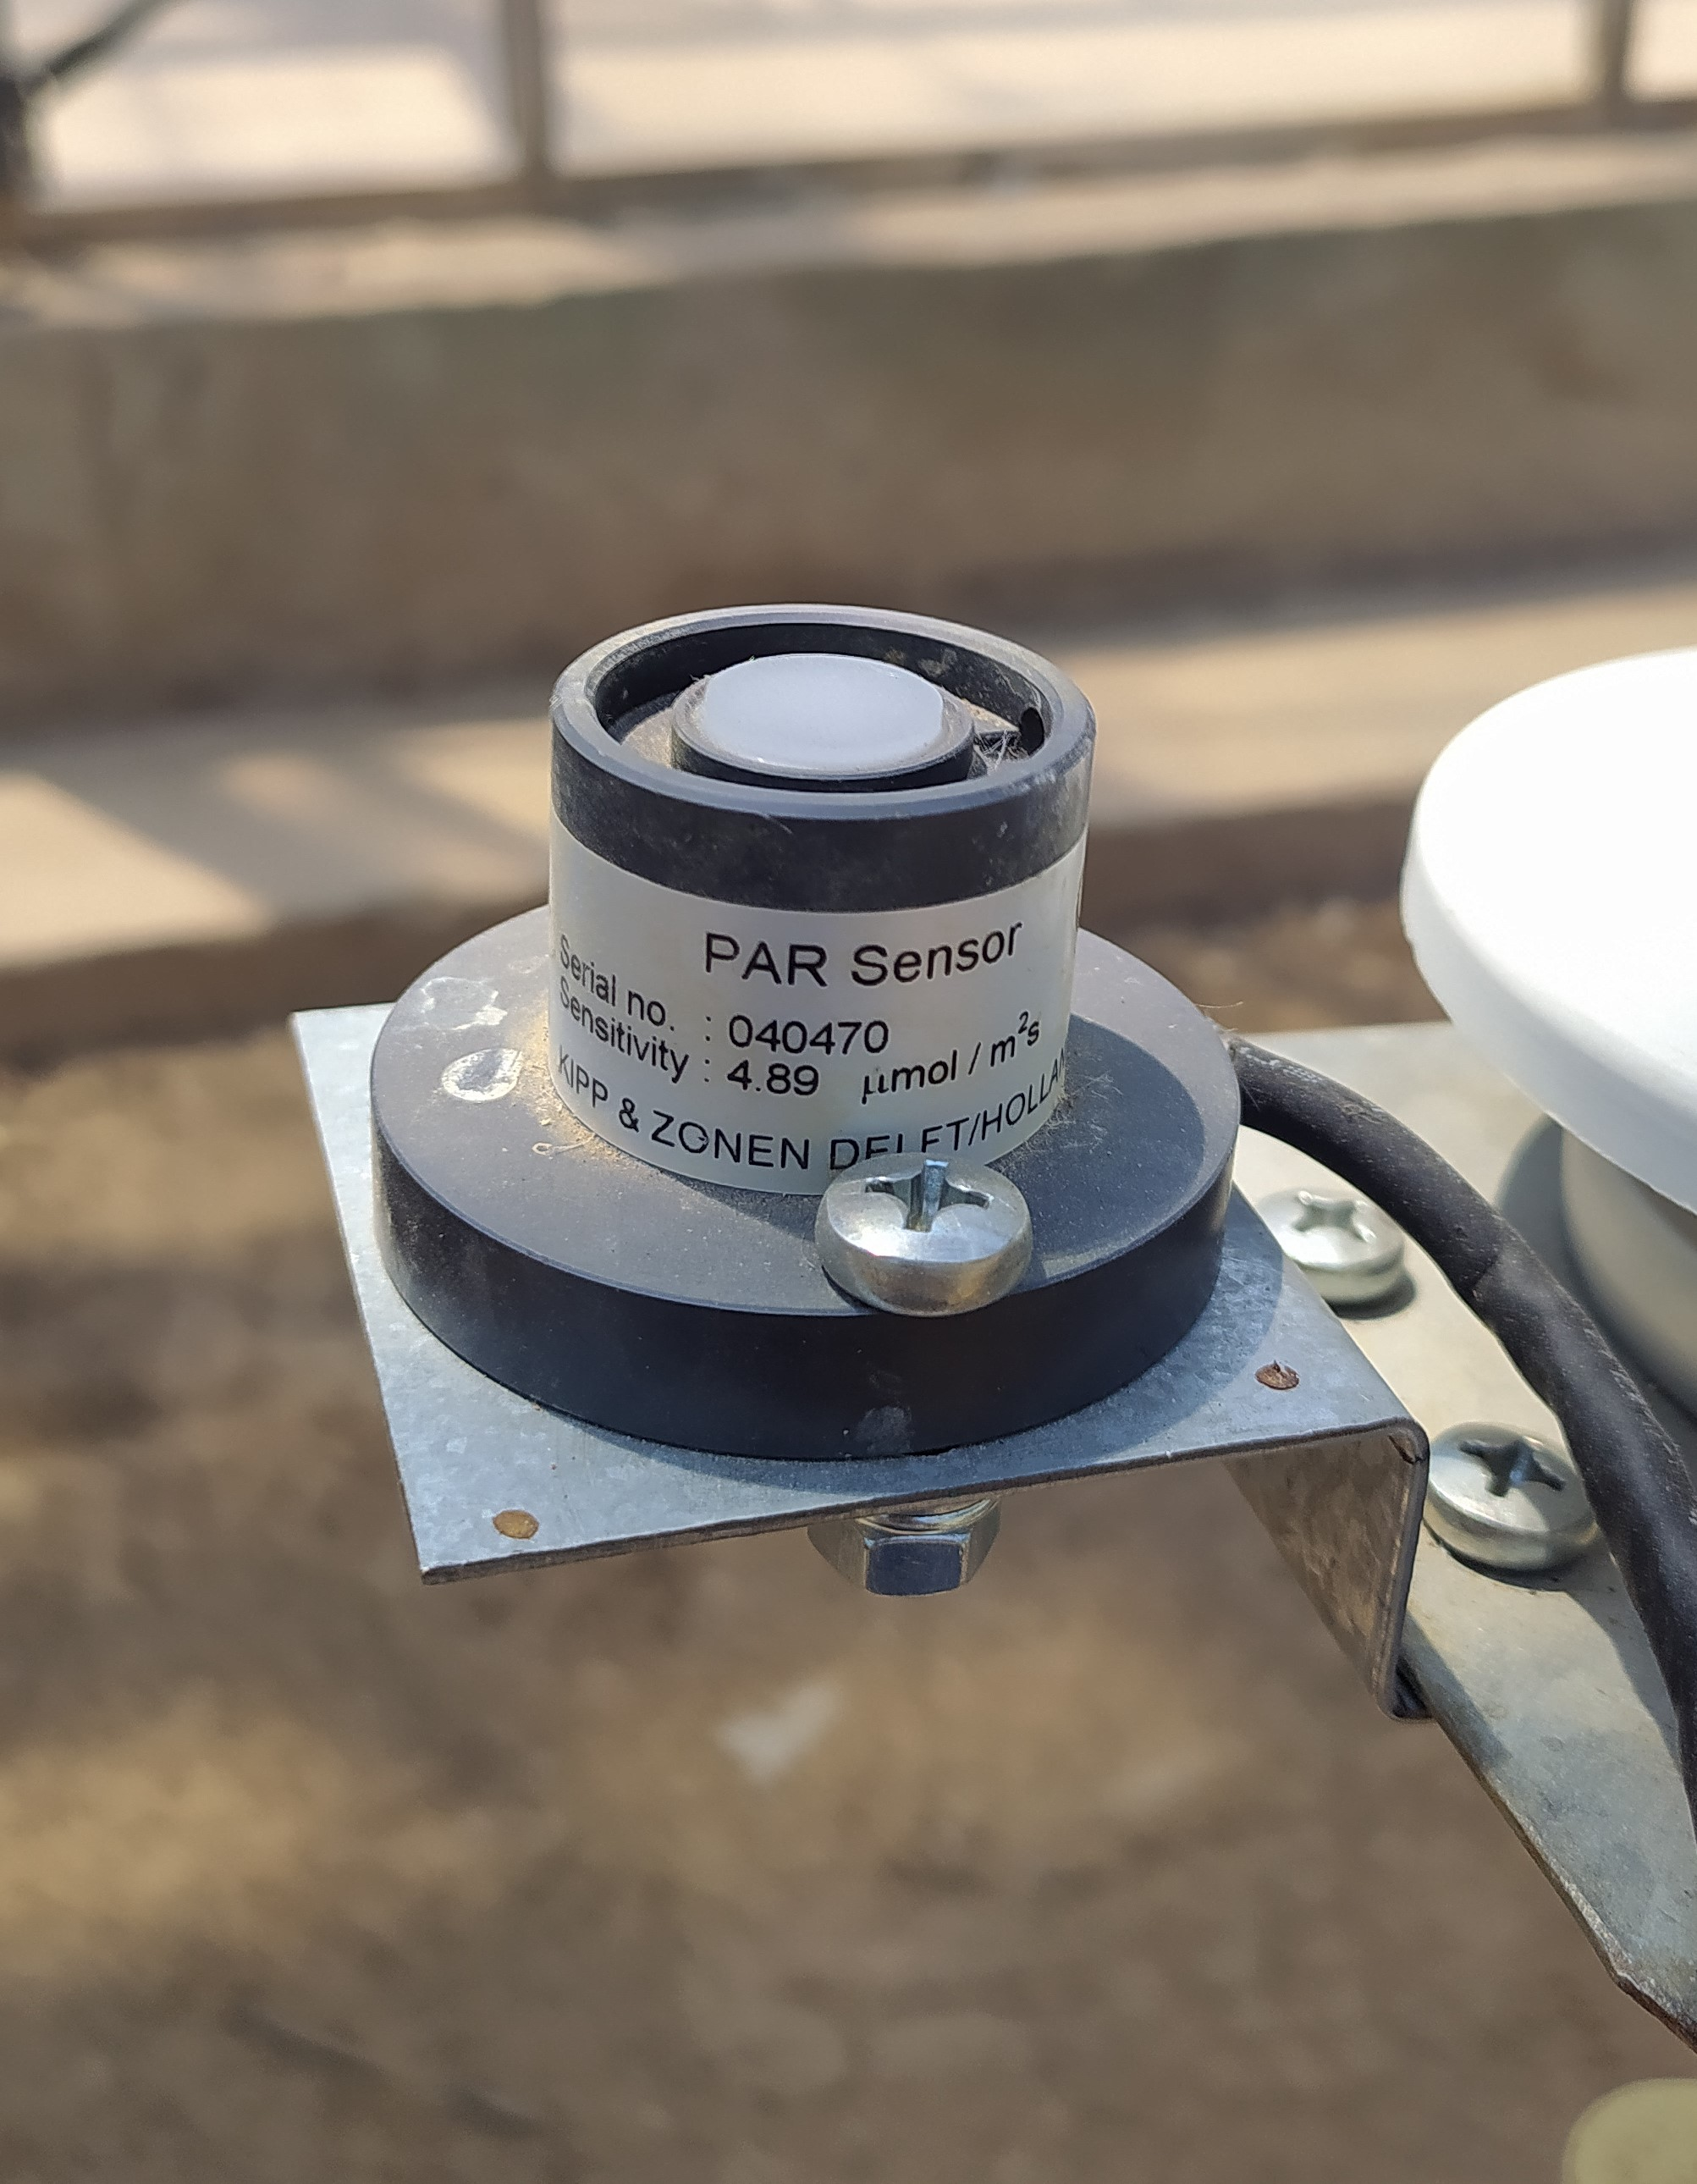
\includegraphics[scale=0.09]{Figures/parlite.jpg}
    \caption{Αισθητήρας φωτοσυνθετικά ενεργής ακτινοβολίας \english{ParLite}.}
    \label{fig_parlite}
\end{figure}

%%%%%%%%%%%%%%%%%%%%%%%%%%%%%%%%%%%%%%%%%%
\subsection{Φωτοβολταϊκές μονάδες}\label{sub_PVs}
Τα φωτοβολταϊκά που χρησιμοποιηθήκαν – \english{BSG-250/49} – στην συγκεκριμένη εργασία αποτελούν μία καινοτομία της 
εταιρείας \english{Brite Hellas S.A.} Όπως έχει ήδη αναφερθεί τα φωτοβολταϊκά δεν επικάθονται στο κάλυμμα του θερμοκηπίου, 
αλλά αποτελούν μέρος αυτού. Συνεπώς, και έχοντας υπόψιν την αναγκαιότητα του φυσικού ηλιακού φωτός για την καλλιέργεια, 
αλλά και τις διάφορες ενεργειακές ανάγκες, όπως η θέρμανση, τα φωτοβολταϊκά αυτά παρουσιάζονται ως ημι-διάφανα, με υψηλή ηλιακή 
διαπερατότητα, αλλά και υψηλό βαθμό σκέδασης του φωτός, γεγονός που δίνει και το πλεονέκτημα αποφυγής επιμέρους έντονων 
σκιάσεων από πιθανά σκελετικά στοιχεία που βρίσκονται κάτω από αυτά. Η ενσωμάτωση των φωτοβολταϊκών στην οροφή του 
θερμοκηπίου που αντικαθιστά τη συμβατική κάλυψη συνάδει με την έννοια των Αγριβολταϊκών, βάσει 
της οποίας η ίδια έκταση αξιοποιείται διπλά, με ταυτόχρονη παραγωγή ενέργειας και τροφίμων. Αυτό μπορεί να συμβάλει στη 
μείωση του κόστους παραγωγής του θερμοκηπίου, καθώς το σύνολο ή μέρος των ενεργειακών αναγκών του θερμοκηπίου δύναται να 
καλυφθεί από τα φωτοβολταϊκά, λειτουργώντας ταυτόχρονα ως υλικό κάλυψης. Σύμφωνα με το τεχνικό φυλλάδιο της εταιρείας 
\english{Brite Hellas} \lcitep{diataksi_bib6}, τα συγκεκριμένα φωτοβολταϊκά ή “ηλιακά τζάμια” διαθέτουν 
μία εγγύηση της διατήρησης της απόδοσής τους για αρκετά χρόνια, με αυτή να μειώνεται στο \SI{85}{\percent} μετά από 25 
χρόνια και στο \SI{82,5}{\percent} μετά από 30.

\vspace{0.4cm}

\noindent \textit{\textbf{Μηχανικά χαρακτηριστικά}}

\vspace{0.2cm}

Οι διαστάσεις της κάθε φωτοβολταϊκής μονάδας είναι \SI{2089}{\milli\meter} μήκος και \SI{1033}{\milli\meter} πλάτος, 
με το πάχος τους να είναι ίσο με \SI{5,5}{\milli\meter} και το βάρος τους ίσο με  \SI{26}{\kilo\gram}. Οι ηλιακές 
κυψελίδες βρίσκονται μεταξύ δύο φύλλων γυαλιού και εντός ενός πιο εύκαμπτου υλικού (\english{POE/EVA}), που δίνει στο 
τζάμι την απαραίτητη ευλυγισία και αντοχή του σε συνθήκες, που θα μπορούσαν να προκαλέσουν ζημιά στο τζάμι, όπως ένα 
σεισμός. Οι κυψελίδες έχουν διαστάσεις \SI{166}{\milli\meter} μήκος και \SI{83}{\milli\meter} πλάτος, ενώ είναι τύπου 
διπλής όψης (\english{bifacial}), αυξάνοντας την παραγωγή ενέργειας, καθώς η παραγωγή ρεύματος βασίζεται στο φως που 
προσπίπτει και στις δύο πλευρές της μονάδας. Ο αριθμός των ηλιακών κυψελίδων που περιέχει το κάθε τζάμι είναι ίσος με 
80. Η διάταξή τους μεταξύ των δύο υαλοπινάκων έχει γίνει σε τέσσερις γραμμές μήκους \SI{1,66}{\meter} η καθεμία 
($20 \cdot 83$ \SI{}{\milli\meter}), με τη μικρή πλευρά κάθε κυψελίδας να είναι παράλληλη προς τη μεγάλη πλευρά του φωτοβολταϊκού. 
Οι αποστάσεις μεταξύ των γραμμών και από τα άκρα κατά μήκος του πλάτους της φωτοβολταϊκής μονάδας είναι ίσες με 
περίπου \SI{6}{\centi\meter}, \SI{7,5}{\centi\meter}, \SI{10,5}{\centi\meter}, \SI{7,5}{\centi\meter} και 
\SI{6}{\centi\meter}. Με βάση τα ανωτέρω, η συνολική επιφάνεια κάθε μονάδας είναι ίση με περίπου \SI{2,12}{\meter\squared}, 
με ενεργή επιφάνεια (συνολική επιφάνεια των ηλιακών κυψελίδων) ίση με \SI{1,102}{\meter\squared} (Πίνακας 
\ref{tab_PV_characteristics}). Στο πίσω μέρος του φωτοβολταϊκού (πλευρά εντός του θερμοκηπίου) υπάρχουν δύο κουτιά 
διακλάδωσης (\english{junction box}) τύπου \english{IP68} με 2 διόδους παράκαμψης (\english{bypass diodes}), ένα για 
τον θετικό και ένα για τον αρνητικό πόλο. Οι κοννέκτορες είναι τύπου \english{MC4}, ενώ το καλώδιο που χρησιμοποιείται 
είναι τύπου \english{TUV Certified} \SI{4}{\milli\meter\squared}. Η θερμοκρασία λειτουργίας τους καλύπτει ένα εύρος 
-40 – \SI{85}{\degreeCelsius}. Τέλος, σύμφωνα με το τεχνικό φυλλάδιο, η σκίαση που προκαλεί κάθε μονάδα είναι της τάξης 
του \SI{51}{\percent}, ενώ η διαπερατότητα στο φάσμα του ορατού της ηλιακής ακτινοβολίας (φωτοσυνθετικά ενεργή ακτινοβολία 
– 400-\SI{700}{\nano\meter}) είναι περίπου \SI{49}{\percent}.

\begin{table}[ht]
    \centering
    \caption{Χαρακτηριστικά φωτοβολταϊκών μονάδων.}\label{tab_PV_characteristics} 
        \begin{tabular}{>{\centering\arraybackslash}m{7.5cm} >{\centering\arraybackslash}m{7.5cm}}
        \toprule
        \textbf{Χαρακτηριστικά} & \textbf{Τιμή} \\
        \midrule
        \multicolumn{2}{c}{\textbf{Φωτοβολταϊκό πλαίσιο}} \\
        \midrule
        Πλάτος & \SI{1.033}{\meter} \\
        Μήκος & \SI{2.089}{\meter} \\ 
        Πάχος & \SI{5,5}{\milli\meter} \\
        Βάρος & \SI{26}{\kilo\gram} \\
        \midrule
        \multicolumn{2}{c}{\textbf{Ηλιακή κυψελίδα}} \\
        \midrule
        Πλάτος & \SI{83}{\milli\meter} \\
        Μήκος & \SI{166}{\milli\meter} \\ 
        Αριθμός & 80\english{pcs} \\
        Τύπος & \english{Bifacial Monocrystalline} \\     
        \bottomrule
    \end{tabular}
\end{table}

\vspace{0.4cm}

\noindent \textit{\textbf{Ηλεκτρικά χαρακτηριστικά}}

\vspace{0.2cm}

Όσον αφορά τα ηλεκτρικά χαρακτηριστικά, αυτά δίνονται για Τυπικές Συνθήκες Δοκιμής (\english{Standard Testing Conditions 
– STC}) (ακτινοβολία \SI{1000}{\watt\per\meter} \& θερμοκρασία κυψελίδας \SI{25}{\degreeCelsius}). Πιο συγκεκριμένα, 
το ρεύμα βραχυκυκλώσεως (\english{Short Circuit Current} – \english{$I_{\text{$sc$}}$}) μετρήθηκε ίσο με 
\SI{11,38}{\ampere}, η τάση ανοιχτού κυκλώματος (\english{Open Circuit Voltage} – \english{$V_{\text{$oc$}}$}) ίση με 
\SI{27,32}{\volt}, το ρεύμα στο σημείο μέγιστης ισχύος (\english{Opt. Operating Current} – \english{$I_{\text{$mpp$}}$}) 
ίσο με \SI{10,81}{\ampere} και η τάση στο σημείο μέγιστης ισχύος (\english{Opt. Operating Voltage} – 
\english{$V_{\text{$mpp$}}$}) ίση με \SI{23,13}{\volt}. Τέλος, η μέγιστη ονομαστική ισχύς κάθε μονάδας είναι ίση με 
\SI{250}{\watt}\english{p}.

Κάνοντας χρήση της σχέσης:

\begin{equation}
    n_{\english{max}} = \frac{P_{\english{max}}}{A_{\english{c}} \cdot E}
    \label{eq_max_PV_performance}
\end{equation}

\noindent όπου \english{$P_{\text{$max$}}$}, είναι η μέγιστη παραγόμενη ισχύς (\SI{250}{\watt}), 
\english{$A_{\text{$c$}}$}, η ενεργός επιφάνεια της μονάδας (\SI{1,102}{\meter\squared}) και \english{$E$}, η ηλιακή 
ακτινοβολία (\SI{1000}{\watt\per\meter\squared} σύμφωνα με τις \english{STC}), μπορούμε να υπολογίσουμε ότι η μέγιστη 
απόδοση του φωτοβολταϊκού είναι περίπου ίση με \SI{22,7}{\percent}.

Παράλληλα, δίνεται η επίδραση της θερμοκρασίας στην μέγιστη ισχύ, το ρεύμα βραχυκυκ\-λώσεως και την τάση ανοιχτού 
κυκλώματος, με τους αντίστοιχους θερμοκρασιακούς συντελεστές να είναι -\SI{0,3904}{\percent\per\kelvin}, 
\SI{0,0268}{\percent\per\kelvin} και -\SI{0,286}{\percent\per\kelvin}, αντίστοιχα. Τέλος, η μέγιστη επιτρεπόμενη τάση 
του συστήματος (\english{Maximum System Voltage}) είναι ίση με \SI{1500}{\volt}, ενώ το μέγιστο επιτρεπόμενο ρεύμα 
(\english{Maximum Series Fuse Rating}) είναι ίσο με \SI{20}{\ampere}.

\vspace{0.4cm}

\noindent \textit{\textbf{Τοποθέτηση}}

\vspace{0.2cm}

Η τοποθέτηση των φωτοβολταϊκών μονάδων ολοκληρώθηκε στις 28/06/2022. Συνολικά στο κάλυμμα του θερμοκηπίου, και στο 
νότιο κεκλιμένο επίπεδο της οροφής κάθε μονάδας ενσωματώθηκαν συνολικά 12 φωτοβολταϊκά. Η γωνία κλίσης των φωτοβολταϊκών 
ως προς το οριζόντιο επίπεδο είναι περίπου ίση με \SI{24}{\degree}, ίση δηλαδή με την γωνία κλίσης της οροφής. Το νότιο 
τμήμα της οροφής επιλέχθηκε με σκοπό την αύξηση της παραγωγής ενέργειας, ιδιαίτερα το χειμώνα, όπου ο ήλιος βρίσκεται σε 
χαμηλό ύψος. Πιο συγκεκριμένα, 8 από τα 12 φωτοβολταϊκά τζάμια ενσωματώθηκαν στη οροφή της βόρειας κατασκευαστικής μονάδας, 
με την μεγάλη τους πλευρά να είναι παράλληλη προς τον κορφιά (κατεύθυνση ανατολής-δύσης), καλύπτοντας περίπου 
\SI{17,2}{\meter\squared} ή το \SI{67}{\percent} της νότιας πλευράς της οροφής. Τα υπόλοιπα 4 βρίσκονται στην οροφή της 
διπλανής μονάδας, καλύπτοντας περίπου \SI{8,6}{\meter\squared} ή το \SI{34}{\percent} της νότιας πλευράς της οροφής. 
Λαμβάνοντας υπόψη την ημι-διαφάνεια των φωτοβολταϊκών, καθώς και το μέγεθος και τον συνολικό αριθμό των ηλιακών κυψελίδων, 
η συνολική ενεργός επιφάνεια (συνολική επιφάνεια που καλύπτουν οι ηλιακές κυψελίδες) ισούται με \SI{8,8}{\meter\squared} 
για την βόρεια κατασκευαστική μονάδα, και με \SI{4,4}{\meter\squared} για την νότια, με τα αντίστοιχα ποσοστά κάλυψης της 
οροφής να είναι \SI{34,4}{\percent} και \SI{17,2}{\percent}.

Με βάση τις διαστάσεις του θερμοκηπίου (Πίνακας \ref{tab_greenhouse_characteristics}) και των φωτοβολταϊκών (Πίνακας 
\ref{tab_PV_characteristics}), και λαμβάνοντας υπόψη μία μικρή επικάλυψη των πλαισίων κατά την τοποθέτηση, σύμφωνα με 
την οποία το μήκος των φωτοβολταϊκών μειώθηκε κατα $\sim$\SI{4}{\milli\meter}, μπορούν να θεωρηθούν 8 διαθέσιμες θέσεις 
για τα φωτοβολταϊκά στην οροφή του θερμοκηπίου, με τις θέσεις που καλύπτονται στη βόρεια κατασκευαστική μονάδα να είναι 
1 έως 8 (Εικόνα \ref{fig_PVs_greenhouse}α), ενώ για τη νότια θερμοκηπιακή μονάδα, οι θέσεις που καλύπτονται να είναι 3, 
4 (κοντά στη δυτική πλευρά του θερμοκηπίου) και 7, 8 (κοντά στην ανατολική πλευρά του θερμοκηπίου) (Εικόνα 
\ref{fig_PVs_greenhouse}β).

Από τις 28/05/2023, και μετά από καταστροφή δύο από τις οχτώ φωτοβολταϊκές μονάδες λόγω ισχυρών ανέμων στην περιοχή, 
τα φωτοβολταϊκά στις θέσεις 1 και 2 (σύμφωνα με την παραπάνω αρίθμηση), απομακρύνθηκαν και αντικαταστάθηκαν με απλό 
υαλοπίνακα, με την αλλαγή αυτή να λαμβάνεται υπόψη στην συνέχεια των πειραμάτων.

\begin{figure}[ht]
    \centering
    \begin{subfigure}{0.5\textwidth}
        \centering
        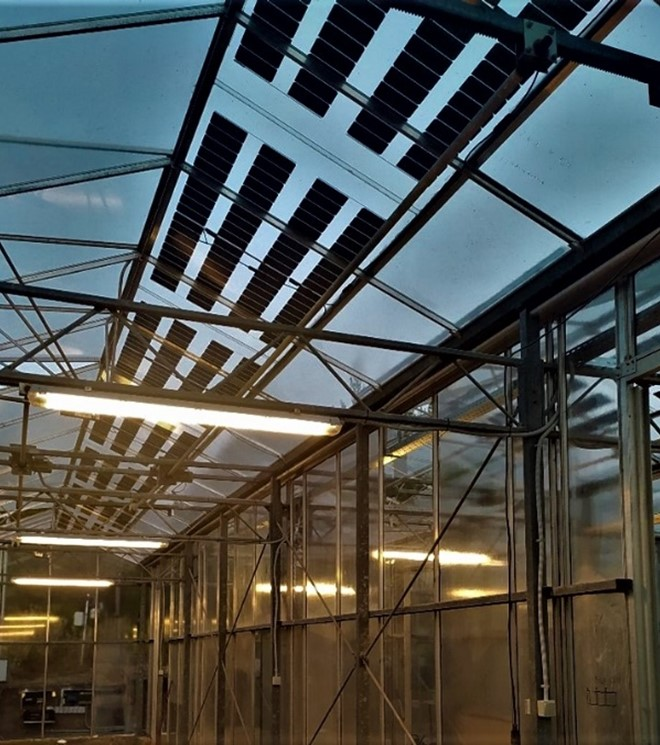
\includegraphics[width=0.8\linewidth, height=80mm]{Figures/PVs_northern.jpg}
        \caption*{(α)}{}
    \end{subfigure}%
    \begin{subfigure}{0.5\textwidth}
        \centering
        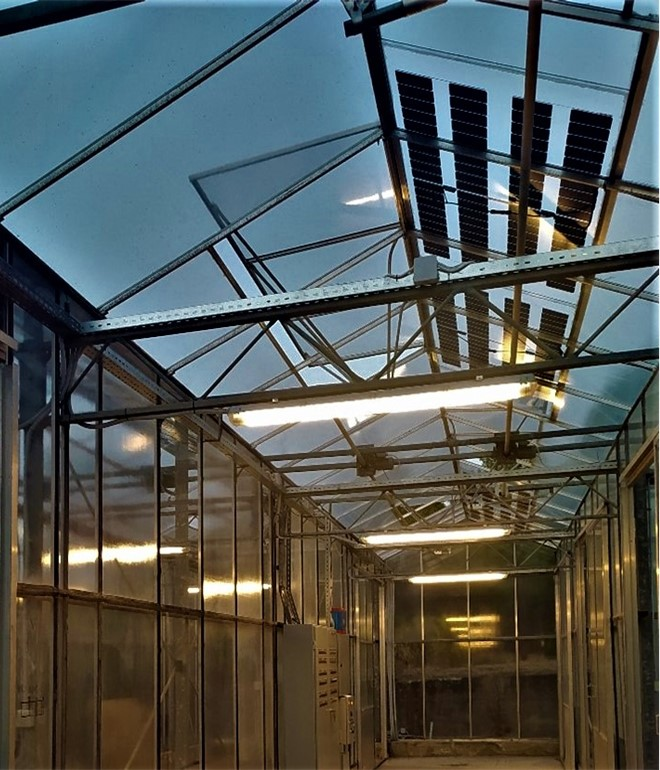
\includegraphics[width=0.8\linewidth, height=80mm]{Figures/PVs_southern.jpg}
        \caption*{(β)}{}
    \end{subfigure}%
    \caption{Φωτοβολταϊκά πλαίσια ενσωματωμένα στο νότιο κεκλιμένο επίπεδο της οροφής του θερμοκηπίου: (α) βόρεια 
    κατασκευαστική μονάδα (β) νότια κατασκευαστική μονάδα.}
    \label{fig_PVs_greenhouse}
\end{figure}

\pagebreak

\noindent \textit{\textbf{Σύνδεση}}

\vspace{0.2cm}

Τα φωτοβολταϊκά κατά την αρχική τους τοποθέτηση συνδέθηκαν με τέτοιο τρόπο ώστε να σχηματίζουν τρείς τετράδες. Κάθε 
τετράδα είναι συνδεδεμένη σε σειρά και συνεπώς ισχύουν (βάσει του τεχνικού φυλλαδίου):

\begin{equation}
    \english{I_{mmp,1-4} = I_{mmp,1} = I_{mmp,2} = I_{mmp,3} = I_{mmp,4} = 10.81 \, A}
    \label{eq_I_mmp_1_4}
\end{equation}

\begin{equation}
    \english{V_{mmp,1-4} = V_{mmp,1} + V_{mmp,2} + V_{mmp,3} + V_{mmp,4} = 4 \cdot 23.13 \, V = 92.52 \, V}
    \label{eq_V_mmp_1_4}
\end{equation}

\noindent ενώ η μέγιστη συνολική ισχύς κάθε τετράδας (σε \english{STC}) είναι:

\begin{equation}
    \english{P_{max,1-4} = P_{max,1} + P_{max,2} + P_{max,3} + P_{max,4} = 4 \cdot 250 \, W = 1000 \, W}
    \label{eq_P_max_1_4}
\end{equation}

\noindent Οι τρεις αυτές τετράδες συνδέονται στην συνέχεια σε παράλληλη σύνδεση σε έναν ρυθμιστή φόρτισης της μπαταρίας 
που υπάρχει στο σύστημα. Το συνολικό μέγιστο ρεύμα που μπορεί να φτάσει στον ρυθμιστή φόρτισης λόγω της παράλληλης σύνδεσης 
είναι:

\begin{equation}
    \english{I_{mmp,total} = I_{mmp,1} + I_{mmp,2} + I_{mmp,3} = 3 \cdot 10.81 = 32.43 \, A}
    \label{eq_I_total}
\end{equation}

\noindent ενώ για την μέγιστη τιμή της τάσης ισχύει:

\begin{equation}
    \english{V_{mmp,total} = V_{mmp,1} = V_{mmp,2} = V_{mmp,3} = 92.52 \, V}
    \label{eq_V_total}
\end{equation}

\noindent Τέλος, η συνολική ονομαστική παραγόμενη ισχύς ισούται με:

\begin{equation}
    \english{P_{max,total} = P_{max,1} + P_{max,2} + P_{max,3} = 3 \cdot 1000 \, W = 3000 \, W}
    \label{eq_P_total}
\end{equation}

Ο ρυθμιστής φόρτισης είναι υπεύθυνος για την φόρτιση μίας επαναφορτιζόμενης μπαταρίας \SI{12}{\volt}, η οποία μέσω 
του αντιστροφέα τάσης (\english{inverter}) τροφοδοτεί το θερμοκήπιο με ενέργεια. Τα στοιχεία που λαμβάνουν το παραγόμενο 
ρεύμα από τα φωτοβολταϊκά είναι οι διάφοροι αισθητήρες εντός και εκτός θερμοκηπίου, ο \english{datalogger}, οι πρίζες, 
τα φώτα και ο κινητήρας των παραθύρων της πειραματικής κατασκευαστικής μονάδας του θερμοκηπίου, καθώς και η ενέργεια που 
απαιτείται στον σταθμό που αφορά το δίκτυο του θερμοκηπίου.

Με την απομάκρυνση των δύο φωτοβολταϊκών μονάδων, όπως προαναφέρθηκε, ήταν απαραίτητο και βάσει των χαρακτηριστικών 
λειτουργίας των υπόλοιπων στοιχείων του συστήματος (π.χ. ρυθμιστής φόρτισης) να γίνει αναδιαμόρφωση την σύνδεσης των 
φωτοβολταϊκών. Συνεπώς, τα δέκα εναπομείναντα φωτοβολταϊκά συνδέθηκαν σε δύο πεντάδες (πρώτα σε σειρά και στην συνέχεια 
σε παράλληλη σύνδεση), με συνολική τάση εξόδου, σύμφωνα με τις σχέσεις \ref{eq_V_mmp_1_4} και \ref{eq_V_total}, και ως 
προς την τάση ανοιχτού κυκλώματος (ίση με \SI{27,32}{\volt}), ίση με \SI{136,6}{\volt}. Η τιμή αυτή δεν ξεπερνά την 
μέγιστη τάση εισόδου του ρυθμιστή φόρτισης (ίση με \SI{150}{\volt}), διατηρώντας την ασφάλεια του συστήματος.

%%%%%%%%%%%%%%%%%%%%%%%%%%%%%%%%%%%%%%%%%%
\subsection{Λοιπά στοιχεία φωτοβολταϊκού συστήματος}\label{sub_loipa_PVs}

\noindent \textit{\textbf{Ρυθμιστής φόρτισης}}

\vspace{0.2cm}

Όσον αφορά τον ρυθμιστή φόρτισης του φωτοβολταϊκού συστήματος, πρόκειται για τον \english{SmartSolar MPPT 150/70 – 
MC4 VE.Can} της εταιρείας \english{Victron Energy} (Εικόνα \ref{fig_solar_charger}). Η συσκευή αυτή έχει το πλεονέκτημα 
της ταχείας παρακολούθησης του σημείου μέγιστης ισχύος, με αποτέλεσμα, σε περιπτώσεις νεφοκάλυψης και συνεχούς μεταβολής 
της έντασης του ηλιακού φωτός, να βελτιώνει την κατανάλωση ενέργειας έως και \SI{30}{\percent} σε σχέση με άλλους ρυθμιστές, 
ενώ ταυτόχρονα σε περιπτώσεις σκίασης, όπου η χαρακτηριστική καμπύλη ισχύος – τάσης μπορεί να εμφανίζει πολλαπλά σημεία 
μέγιστης ισχύος, ο συγκεκριμένος ρυθμιστής περιέχει έναν αλγόριθμο που του επιτρέπει να κλειδώνει το βέλτιστο από αυτά τα 
σημεία. Η απόδοση ισχύος του ρυθμιστή παρουσιάζεται να είναι μεγαλύτερη του \SI{98}{\percent}. Ακόμη, αν και δεν περιέχει 
ανεμιστήρα ψύξης, η ηλεκτρονική του προστασία είναι υψηλή, καθώς παρέχεται προστασία από μεγάλη αύξηση της θερμοκρασίας, 
παρατηρούμενη από ενσωματωμένο αισθητήρα θερμοκρασίας, με την μείωση της ισχύος. Προστασία παρέχεται επίσης, από 
βραχυκύκλωμα στα φωτοβολταϊκά πλαίσια, σε περιπτώσεις αντίστροφης πολικότητας αυτών, αλλά και σε περιπτώσεις ανάστροφου 
ρεύματος. Παράλληλα, το ενσωματωμένο στον ρυθμιστή \english{Bluetooth} παρέχει δυνατότητες ασύρματης ρύθμισης, ζωντανής 
(\english{real-time}) παρακολούθησης της παραγόμενης από τα φωτοβολταϊκά ισχύος, του ρεύματος και της τάσης αυτών, και 
του ρεύματος και της τάσης που αποδίδει η μπαταρία, ενημέρωσης και συγχρονισμό όλων των πιθανών έξυπνων ρυθμιστών φόρτισης 
στο σύστημα. Για την ενσύρματη σύνδεση και την αποστολή δεδομένων σε ηλεκτρονικό υπολογιστή, είτε με απευθείας σύνδεση, 
είτε με συσκευή για αποστολή δεδομένων μέσω δικτύου, ο ρυθμιστής παρέχει δύο επιλογές, είτε άμεσα μέσω σχετικής θύρας 
(\english{VE.Direct}), είτε μέσω ενός συστήματος σειριακού διαύλου \english{CAN (VE.Can)}. Τέλος, ο ρυθμιστής ενσωματώνει 
προγραμματιζόμενο ρελέ για την απενεργοποίησή του μέσω ειδοποίησης ή για άλλα συμβάντα \lcitep{diataksi_bib7}.

\begin{figure}[ht]%
    \centering
    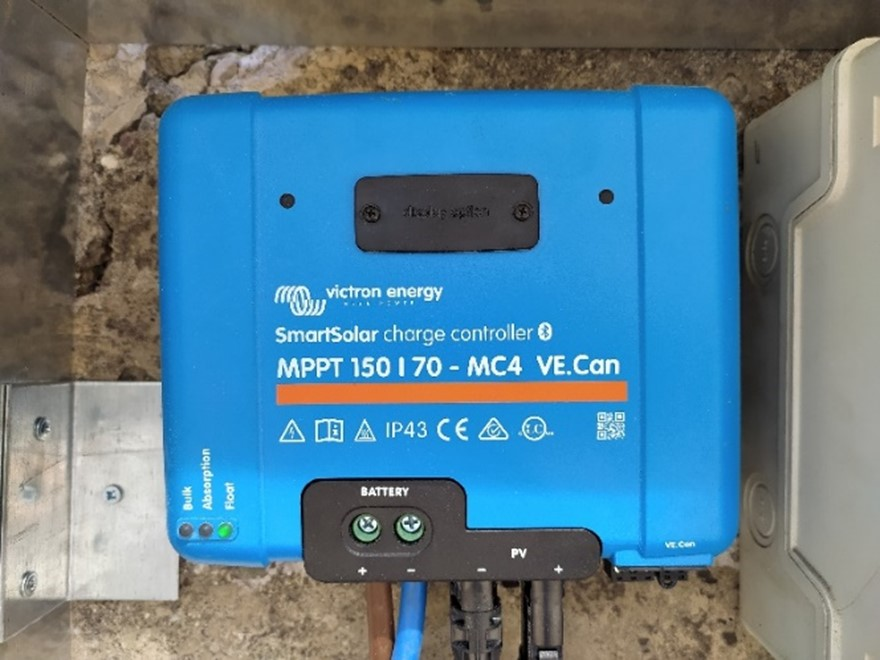
\includegraphics[scale=0.85]{Figures/solar_charger.jpg}
    \caption{Ρυθμιστής φόρτισης \english{SmartSolar MPPT 150/70 – MC4 VE.Can} του φωτοβολταϊκού συστήματος.}
    \label{fig_solar_charger}
\end{figure}

\pagebreak

\noindent \textit{\textbf{Αντιστροφέας Τάσης (\english{Inverter})}}

\vspace{0.2cm}

Για την μετατροπή του παραγόμενου από τα φωτοβολταϊκά ρεύματος από συνεχές (\english{DC}) σε εναλλασσόμενο (\english{AC}) 
χρησιμοποιείται ο αντιστροφέας τάσης \english{MMS-E Series Inverter/Charger} της εταιρείας \english{Magnum Energy} 
(Εικόνα \ref{fig_inverter}). Ο \english{MMS-E Series Inverter/Charger} είναι ένας αντιστροφέας καθαρού ημιτονοειδούς 
κύματος (\english{Pure Sine}) με την δυνατότητα να ανταποκρίνεται σε ένα μεγάλος πλήθος συσκευών. Χαρακτηρίζεται ως 
υβριδικός, καθώς έχει την δυνατότητα να τροφοδοτεί τα διάφορα στοιχεία, είτε μέσω της ενέργειας από τα φωτοβολταϊκά πάνελ, 
είτε μέσω του δημόσιου δικτύου ηλεκτροδότησης.

H τάση εισόδου του είναι μεταξύ 10 και \SI{17}{\volt} (\english{DC}), ενώ η αντίστοιχη τιμή εξόδου είναι \SI{230}{\volt} 
(\english{AC}) $\pm$\SI{5}{\percent}. Επιπλέον, η ισχύς εξόδου του (\english{Output Power}) είναι \SI{900}{\watt}, ενώ η 
μέγιστη ισχύς (για λειτουργία μερικών λεπτών) (\english{Peak Watts}) είναι \SI{1600}{\watt}. Το ρεύμα και η συχνότητα 
εξόδου είναι \SI{3,9}{\ampere} και 50 $\pm$ \SI{0,1}{\hertz}, αντίστοιχα, ενώ η απόδοσή του φτάνει το \SI{87}{\percent}. 
Τέλος, οι περιβαλλοντικές συνθήκες λειτουργίας του (θερμοκρασία και σχ. υγρασία) είναι -20 – \SI{60}{\degreeCelsius} και 
0 – \SI{95}{\percent} \lcitep{diataksi_bib8}.

\begin{figure}[ht]%
    \centering
    
\includegraphics[scale=0.9]{Figures/inverter.jpg}
    \caption{Αντιστροφέας τάσης \english{MMS-E Series Inverter/Charger} του φωτοβολταϊκού συστήματος.}
    \label{fig_inverter}
\end{figure}

\noindent \textit{\textbf{Μπαταρία}}

\vspace{0.2cm}

Για την αποθήκευση της παραγόμενης από τα φωτοβολταϊκά ενέργειας, αλλά και της ενέργειας που προέρχεται από το δίκτυο, 
εφόσον τα φωτοβολταϊκά δεν μπορούν να ανταποκριθούν (περιπτώσεις πλήρους νεφοκάλυψης), στο σύστημα χρησιμοποιείται η 
μπαταρία \english{Deep Cycle AGM} (Εικόνα \ref{fig_battery}) της εταιρείας \english{NorthBatt}, με τον σχεδιασμό της 
συγκεκριμένης μπαταρίας να ανταποκρίνεται σε εκατοντάδες κύκλους φόρτισης-εκφόρτισης, εξαιτίας των υλικών κατασκευής της. 
Για εφαρμογές σε κατάσταση \english{Float}, η διάρκεια ζωής της μπαταρίας είναι μεγαλύτερη των 10 ετών, με 1200 κύκλους 
για χρήση σε θερμοκρασία \SI{25}{\degreeCelsius}, ενώ συγχρόνως έχει την δυνατότητα αποθήκευσης 3 έως 6 μηνών πριν την 
επαναφόρτιση, χωρίς καθόλου απώλειες στην απόδοσή της.

Όσον αφορά τα τεχνικά της χαρακτηριστικά, πρόκειται για μία μπαταρία \SI{12}{\volt}, χωρητικότητας \SI{150}{\ampere\hour} 
με ρυθμό εκφόρτισης \english{C20} ή \SI{180}{\ampere\hour} με ρυθμό εκφόρτισης \english{C100} και μέγιστου ρεύματος 
εκφόρτισης \SI{900}{\ampere}. Στα χαρακτηριστικά φόρτισης της μπαταρίας διακρίνονται δύο καταστάσεις, η κατάσταση 
\english{Float} με τάση στα \SI{13,7}{\volt} $\pm$ \SI{0,1}{\volt} και η κατάσταση \english{Cyclic} με τάση στα 
\SI{14,7}{\volt} $\pm$ \SI{0,1}{\volt} και μέγιστο και ελάχιστο ρεύμα ίσο με \SI{0,3}{\centi\ampere} και 
\SI{0,1}{\centi\ampere}, αντίστοιχα \lcitep{diataksi_bib9}. 

\begin{figure}[ht]%
    \centering
    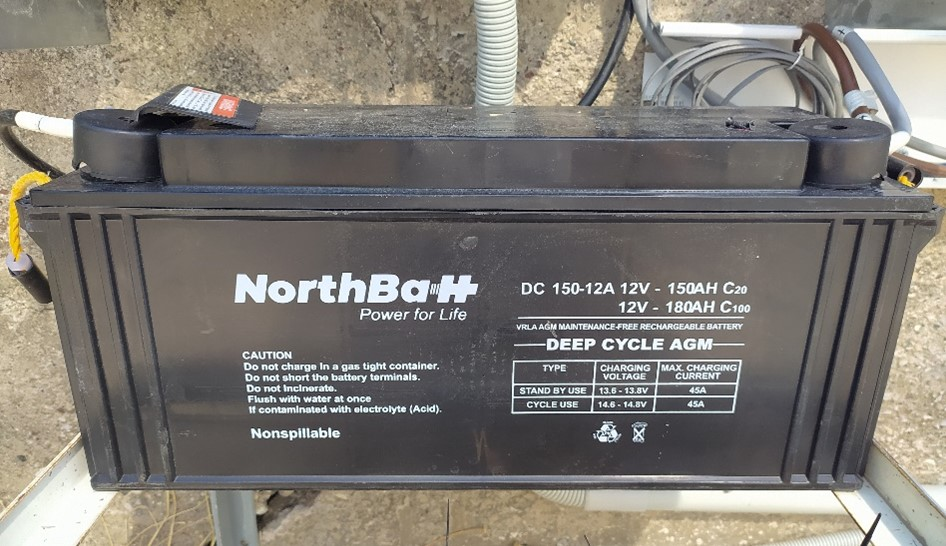
\includegraphics[scale=0.9]{Figures/battery.jpg}
    \caption{Mπαταρία \english{Deep Cycle AGM} του φωτοβολταϊκού συστήματος.}
    \label{fig_battery}
\end{figure}

\noindent \textit{\textbf{Μετρητές}}

\vspace{0.2cm}

Ένα από τα σημαντικότερα σημεία του συστήματος είναι αυτό της μέτρησης. Έχει επιτευχθεί η λήψη μετρήσεων της ενεργού 
και άεργης ισχύος, του ρεύματος, της τάσης, της συχνότητας, του συντελεστή ισχύος, καθώς και της συνολικής κατανάλωσης 
ενέργειας του συστήματος. Οι μετρήσεις αυτές αφορούν δύο διαφορετικά σημεία, δηλαδή όλα τα παραπάνω μετρούνται για την 
παροχή από τα φωτοβολταϊκά, αλλά και την παροχή ενέργειας από το δημόσιο δίκτυο ηλεκτροδότησης. Το σύστημα μετρήσεων 
αποτελείται από έναν ασύρματο τριφασικό ενεργειακό μετρητή (\english{DinRail 3-Phase Advanced}) της εταιρείας 
\english{Meazon} (Εικόνα \ref{fig_dinrail}), ο οποίος χρησιμοποιείται για την μέτρηση και τον έλεγχο ενός τριφασικού 
φορτίου ή τριών μονοφασικών, τρεις \english{Split-Core} μετασχηματιστές ρεύματος (Εικόνες \ref{fig_split_core}α \& 
\ref{fig_split_core}β), με δυνατότητα μέτρησης έως και \SI{2400}{\ampere} ανά φάση, και μίας \english{Linux} συσκευής 
(\english{Janus Gateway}) (Εικόνα \ref{fig_janus}) για την ανάκτηση, την συγκέντρωση και την μεταφορά δεδομένων από 
τις παραπάνω συσκευές προς τις διαδικτυακές υπηρεσίες ανάλυσης μέσω \english{Ethernet}.

Ο μετρητής \english{DinRail 3-Phase Advanced} ενδείκνυται για την παρακολούθηση σε πραγματικό χρόνο, τόσο της 
καταναλισκόμενης, όσο και της παραγόμενης ισχύος. Είναι εξοπλισμένος με ενσωματωμένο \english{datalogger} με δυνατότητα 
αποθήκευσης των δεδομένων για 2 με 3 εβδομάδες, με χρονικό βήμα καταγραφής έως και 1 δευτερόλεπτο. Τα καταγραφέντα 
δεδομένα μεταφέρονται μέσω δικτύου \english{ZigBee} στο \english{Janus Gateway} και από εκεί αποστέλλονται στο 
\english{Cloud}.

\begin{figure}[ht]%
    \centering
    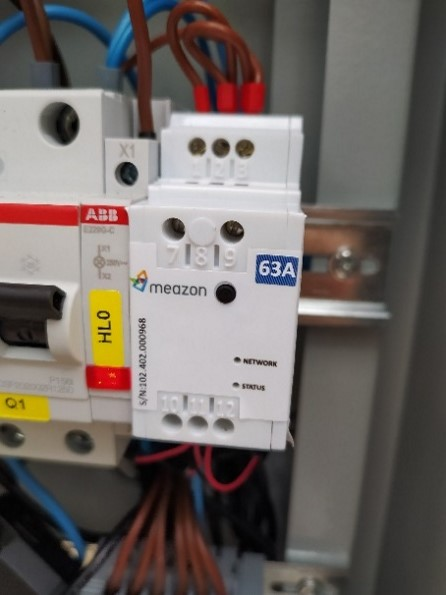
\includegraphics[scale=1]{Figures/DinRail.jpg}
    \caption{Tριφασικός ενεργειακός μετρητής (\english{DinRail 3-Phase Advanced}).}
    \label{fig_dinrail}
\end{figure}

\begin{figure}[ht]
    \centering
    \begin{subfigure}{0.5\textwidth}
        \centering
        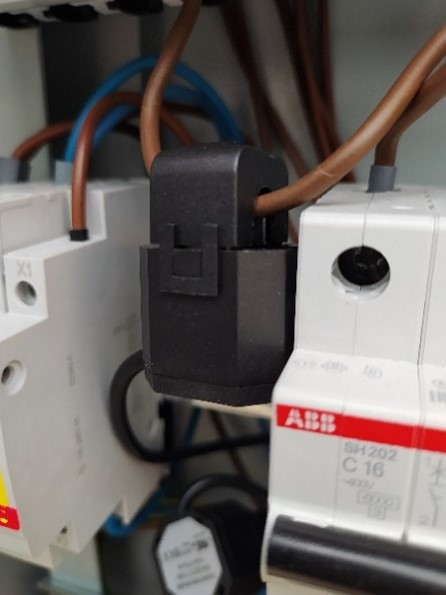
\includegraphics[scale=1]{Figures/split_core_a.jpg}
        \caption*{(α)}{}
    \end{subfigure}%
    \begin{subfigure}{0.5\textwidth}
        \centering
        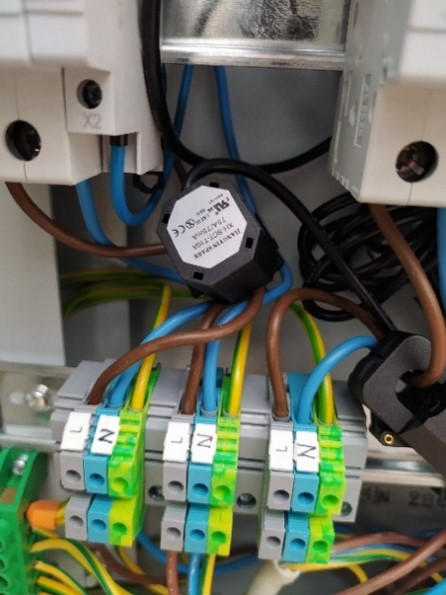
\includegraphics[scale=1]{Figures/split_core_b.jpg}
        \caption*{(b)}{}
    \end{subfigure}%
    \caption{\english{Split-Core} μετασχηματιστές ρεύματος}
    \label{fig_split_core}
\end{figure}

\begin{figure}[ht]%
    \centering
    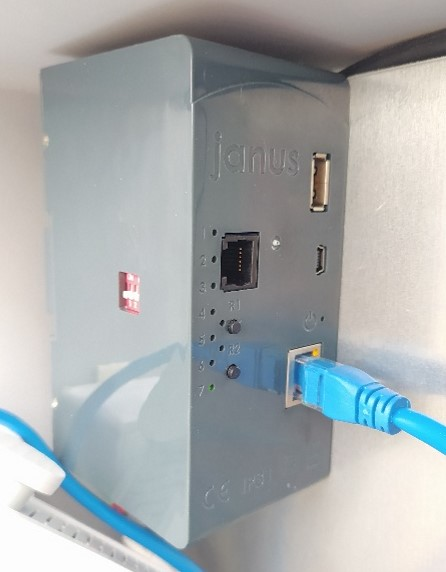
\includegraphics[scale=1]{Figures/janus.jpg}
    \caption{Συσκευή \english{Janus Gateway}.}
    \label{fig_janus}
\end{figure}

Τέλος, το παραπάνω μετρητικό σύστημα συνοδεύεται από μία διαδικτυακή εφαρμογή \english{UI}, για την ζωντανή 
παρακολούθηση των καταγραφών υπό μορφή γραφημάτων, αλλά και την λήψη των δεδομένων σε αρχεία \english{CSV}. 

%%%%%%%%%%%%%%%%%%%%%%%%%%%%%%%%%%%%%%%%%%
%%%%%%%%%%%%%%%%%%%%%%%%%%%%%%%%%%%%%%%%%%
\clearpage
\vspace*{6.5cm}
\sloppy
\section{Μοντέλο νευρωνικού δικτύου για προβλέψεις μικροκλίματος θερμοκηπίου}\label{sec_NN_model}
\fussy

Η μοντελοποίηση του μικροκλίματος ενός θερμοκηπίου διαφέρει ανάλογα με τον σκοπό. Υπάρχουν δύο κύριες κατηγορίες μοντέλων, 
τα φυσικά, τα οποία χρησιμοποιούνται κυρίως αν βασικός στόχος είναι η μελέτη και η γνώση των φυσικών διαδικασιών που 
λαμβάνουν χώρα μέσα στο θερμοκήπιο, και τα μοντέλα “μαύρου κουτιού” (“\english{Black-Box models}”), αν ο κύριος στόχος 
είναι οι εφαρμογές και ο σχεδιασμός συστημάτων που σχετίζονται με τη διαχείριση του θερμοκηπίου. Η ανάπτυξη ενός φυσικού 
μοντέλου παρουσιάζει υψηλό βαθμό δυσκολίας, ιδίως εξαιτίας του γεγονότος ότι το θερμοκήπιο αποτελεί ένα πολύπλοκο, μη 
γραμμικό σύστημα, με τα συγκεκριμένα μοντέλα να βασίζονται κυρίως στους νόμους της θερμοδυναμικής και της μεταφοράς 
θερμότητας και μάζας, με αποτέλεσμα παράμετροι όπως η ηλιακή ακτινοβολία και παράγοντες που σχετίζονται με τους παραπάνω 
νόμους να πρέπει να υπολογίζονται με υψηλή ακρίβεια \lcitep{neural_bib5,neural_bib6,neural_bib7}. Από την άλλη πλευρά, τα 
μοντέλα “μαύρου κουτιού” βασίζονται στη διαδικασία αναγνώρισης συστημάτων (\english{System Identification – SI – process}). 
H διαδικασία αναγνώρισης συστημάτων είναι μια μεθοδολογία που εξαρτάται κυρίως από πειραματικά δεδομένα εισόδου και εξόδου. 
Αυτά τα μοντέλα παρέχουν μια αποτελεσματική και ακριβή περιγραφή της συμπεριφοράς διάφορων παραμέτρων χωρίς την ανάγκη 
μοντελοποίησης των εσωτερικών διαδικασιών του συστήματος \lcitep{neural_bib8}. Η ανάπτυξη ενός τέτοιου μοντέλου απαιτεί 
μια διαδικασία που περιλαμβάνει μετρήσεις σήματος για συγκεκριμένη χρονική στιγμή, την επιλογή δομής μοντέλου, την επιλογή 
και τον ορισμό του τρόπου βάσει του οποίου θα υπολογιστούν οι κατάλληλες παράμετροι του μοντέλου, και την επικύρωση και 
αξιολόγηση του μοντέλου χρησιμοποιώντας ένα σύνολο δεδομένων διαφορετικό από αυτό που χρησιμοποιήθηκε για το υπόλοιπο της 
διαδικασίας \lcitep{neural_bib9}.

Όπως αναφέρθηκε παραπάνω, τα θερμοκήπια είναι δυναμικά, μη γραμμικά και υψηλής πολυπλοκότητας συστήματα με συνεχείς 
αλληλεπιδράσεις μεταξύ των μεταβλητών του μικροκλίματός τους. Ο συνδυασμός των παραπάνω με την ανάγκη για δημιουργία 
μοντέλων που θα εφαρμοστούν άμεσα για τον έλεγχο του θερμοκηπίου δίνει στα μοντέλα μαύρου κουτιού, και γενικότερα στις 
τεχνικές της τεχνητής νοημοσύνης ιδιαίτερη αξία. Μία από αυτές τις τεχνικές είναι η μοντελοποίηση και ο έλεγχος του 
μικροκλίματος του θερμοκηπίου μέσω νευρωνικών δικτύων (\english{Neural Networks – NNs}). Τα νευρωνικά δίκτυα βασίζονται 
στη λογική του βιολογικού νευρικού συστήματος, όπου τα σήματα που λαμβάνονται από ένα κύτταρο μέσω ενός δικτύου “καλωδίων” 
που ονομάζονται δενδρίτες, μεταφέρονται σε διαφορετικούς νευρώνες μέσω μιας ίνας που ονομάζεται νευροάξονας (ή άξονας). 
Η σύνδεση ενός άξονα με έναν δενδρίτη ενός διαφορετικού κυτταρικού σώματος ονομάζεται νευρική σύναψη. Η κατάσταση ενός 
τέτοιου συστήματος εξαρτάται σε μεγάλο βαθμό από τον τρόπο διάταξης των παραπάνω, με τις δυνάμεις μεταξύ των συνάψεων να 
ενισχύονται ή να εξασθενούν ανάλογα με τη διαδικασία της μάθησης \lcitep{neural_bib10}. Σε ένα Τεχνητό Νευρωνικό Δίκτυο 
(\english{Artificial Neural Network – ANN}), τα σήματα μεταφέρονται από τους κόμβους (νευρώνες) του επιπέδου εισόδου 
(\english{input layer}) στους κόμβους ενός “κρυφού” επιπέδου (\english{hidden layer}), οι οποίοι ενεργοποιούνται ανάλογα 
με τον συντελεστή βαρύτητάς τους, μεταφέροντας τελικά το σήμα στους κόμβους ενός τελικού επιπέδου που ονομάζεται επίπεδο 
εξόδου (\english{output layer}). Η παραπάνω διαδικασία για την εξαγωγή αξιόλογων αποτελεσμάτων απαιτεί προσεκτική επιλογή 
του τρόπου σύνδεσης των νευρώνων (τοπολογία), ενός αλγορίθμου εκπαίδευσης σύμφωνα με τον οποίο θα πραγματοποιηθεί η 
διαδικασία της μάθησης, του αριθμού των κρυφών επιπέδων και κόμβων, και των μεταβλητών που θα εισάγουν την πληροφορία στο 
δίκτυο \lcitep{neural_bib11}.

Τα νευρωνικά δίκτυα χρησιμοποιούνται ευρέως στα θερμοκήπια όχι μόνο για τον έλεγχο, αλλά και για την πρόβλεψη 
μικροκλιματικών παραμέτρων, εξάγοντας αξιοσημείωτα και σαφή αποτελέσματα. Η έρευνα στον συγκεκριμένο τομέα αφορά την 
χρήση διαφορετικών αρχιτεκτονικών για την δημιουργία ενός νευρωνικού δικτύου, όπως η χρήση δικτύων εμπρόσθιας τροφοδότησης 
(\english{feedforward}) ή επαναλαμβανόμενων (\english{recurrent}) νευρωνικών δικτύων, καθώς και διαφορετικών αλγορίθμων 
εκπαίδευσης (\english{training algorithms}). Πιο συγκεκριμένα, οι \english{Singh \& Tiwari} (\citeyear{eisagwgi_NN_bib2}) 
σχεδίασαν και έλεγξαν ένα νευρωνικό δίκτυο εμπρόσθιας τροφοδότησης με μόνο ένα κρυφό επίπεδο, αλλά διαφορετικό αριθμό 
κόμβων με σκοπό να προβλέψουν την θερμοκρασία και την σχετική υγρασία εντός του θερμοκηπίου για μία μέρα μπροστά. Μετά 
από αρκετά πειράματα και με τους κόμβους του κρυφού επιπέδου να κυμαίνονται μεταξύ τριών έως δέκα, διαπιστώθηκε πως η δομή 
με τέσσερις κρυφούς κόμβους εξήγαγε τα καλύτερα αποτελέσματα, με τους συντελεστές προσδιορισμού να είναι ίσοι με 0,980 
και 0,967, για την θερμοκρασία και την σχετική υγρασία, αντίστοιχα. Οι \english{Castañeda \& Castaño} 
(\citeyear{neural_bib12}) δημιούργησαν ένα νευρωνικό δίκτυο πολυστρωματικής αντίληψης 
(\english{Multilayer Perceptron – MLP}), κάνοντας χρήση του \english{Levenberg–Marquardt} ως αλγορίθμου εκπαίδευσης, το 
οποίο μπορεί να προβλέψει την θερμοκρασία εντός του θερμοκηπίου για την χειμερινή και την καλοκαιρινή περίοδο, με σκοπό 
τον έλεγχο του παγετού μέσα στο θερμοκήπιο. Οι αντίστοιχοι συντελεστές προσδιορισμού προέκυψαν ίσοι με 0,9549 και 0,9590. 
Οι \english{Choi et al.} (\citeyear{neural_bib13}) εκπαίδευσαν επίσης ένα νευρωνικό δίκτυο \english{MLP} χρησιμοποιώντας 
τα δεδομένα των εξωτερικών και εσωτερικών συνθηκών του θερμοκηπίου ως μεταβλητές εισόδου, για να προβλέψουν την εσωτερική 
θερμοκρασία και σχετική υγρασία για 10 έως 120 λεπτά αργότερα. Το νευρωνικό δίκτυο αποτελούνταν από τέσσερα κρυφά επίπεδα 
και διαφορετικό αριθμό κόμβων, με σκοπό την πρόβλεψη της θερμοκρασίας και της σχετικής υγρασίας, με τους συντελεστές 
προσδιορισμού να είναι ίσοι με 0,988 και 0,990, αντίστοιχα.

Τα επαναλαμβανόμενα νευρωνικά δίκτυα είναι επίσης ευρέως διαδεδομένα, με την δομή \english{Elman} μεταξύ άλλων να είναι 
η πιο γνωστή. Οι \english{Hongkang et al.} (\citeyear{neural_bib14}) δημιούργησαν ένα δίκτυο \english{Elman} το οποίο 
βασίζεται σε έναν δυναμικό αλγόριθμο εκπαίδευσης οπισθοδιάδοσης (\english{backpropagation training algorithm}). Ως 
μεταβλητές εισόδου, χρησιμοποίησαν παραμέτρους του εσωτερικού περιβάλλοντος, όπως η θερμοκρασία του αέρα και του 
υποστρώματος, η σχετική υγρασία, η συγκέντρωση \english{CO$_2$} και ο φωτισμός. Από αυτό το μοντέλο προέκυψαν συντελεστές 
προσδιορισμού μεγαλύτεροι του 0,9, και πιο συγκεκριμένα οι τιμές τους για την θερμοκρασία και την σχετική υγρασία ήταν 
ίσες με 0,925 και 0,937 αντίστοιχα. Επιπλέον, οι \english{Salah \& Fourati} (\citeyear{neural_bib15}) συνδύασαν ένα δίκτυο 
\english{Elman} με ένα βαθύ πολυστρωματικό νευρωνικό δίκτυο εμπρόσθιας τροφοδότησης για τον έλεγχο του θερμοκηπίου. 
Το πρώτο δίκτυο χρησιμοποιήθηκε για την προσομοίωση της άμεσης δυναμικής των εσωτερικών διεργασιών, ενώ το δεύτερο για 
την αντίστροφη δυναμική. Τέλος, οι \english{Taki et al.} (\citeyear{neural_bib16}) έκαναν μία σύγκριση μεταξύ τριών 
διαφορετικών μοντέλων για την εκτίμηση τριών διαφορετικών θερμοκρασιών μέσα στο θερμοκήπιο, τη θερμοκρασία του αέρα, τη 
θερμοκρασία του εδάφους και την θερμοκρασία των φυτών. Μετά από τη σύγκριση ενός Ακτινικού Δικτύου Βάσης 
(\english{Radial Basis Function – RBF}), ενός \english{MLP} και ενός μοντέλου Μηχανής Διανυσματικής Υποστήριξης 
(\english{Support Vector Machine – SVM}), διαπιστώθηκε ότι το πρώτο παρουσίασε τα καλύτερα αποτελέσματα.

Το παρόν κεφάλαιο της μελέτης στοχεύει στη δημιουργία ενός μοντέλου κάνοντας χρήση των Τεχνητών Νευρωνικών Δικτύων, 
το οποίο μπορεί να προβλέπει τη θερμοκρασία (\english{$T_{\text{$in$}}$}) και τη σχετική υγρασία 
(\english{$RH_{\text{$in$}}$}) εντός του θερμοκηπίου, βασιζόμενο στην εξωτερική θερμοκρασία (\english{$T_{\text{$out$}}$}) 
και τη σχετική υγρασία (\english{$RH_{\text{$out$}}$}), την ταχύτητα του ανέμου (\english{$WS$}), την ηλιακή ακτινοβολία 
(\english{$SR$}), καθώς και την εσωτερική θερμοκρασία και τη σχετική υγρασία έως και μισή ώρα πριν. Μετά από εκτεταμένη 
έρευνα στη βιβλιογραφία τα τελευταία χρόνια, δεν έχει βρεθεί κάποια παρόμοια μελέτη. Στόχος αποτελεί το μοντέλο να εμφανίζει 
όσο το δυνατόν χαμηλότερο μέγιστο σφάλμα μεταξύ των προβλεπόμενων και παρατηρούμενων δεδομένων, ώστε να μπορεί να 
ανταποκριθεί επαρκώς σε ένα σύστημα υποστήριξης λήψης αποφάσεων.

\subsection{Συλλογή δεδομένων και μεθοδολογία}\label{sub_data_method_NN}

Στην μελέτη αυτή χρησιμοποιήθηκε ένα σύνολο δεδομένων περίπου 62 ημερών, από τις 14 Φεβρουαρίου 2022 στις 14:00 μέχρι 
τις 18 Απριλίου 2022 στις 8:10, για την εκπαίδευση και δοκιμή του μοντέλου. Τα δεδομένα λήφθηκαν με χρήση των αισθητήρων 
που περιγράφονται στην Παράγραφο \ref{sub_eksoplismos}, εντός και εκτός του θερμοκηπίου που περιγράφεται στην Παράγραφο 
\ref{sub_thermokipio}. Ο χρόνος εκφράζεται σε Ώρα Ανατολικής Ευρώπης (\english{Eastern European Time – EET}) για την υπό 
μελέτη χρονική περίοδο, ενώ το χρονικό βήμα των δεδομένων (\english{$t_{\text{$s$}}$}) είναι ίσο με 10 λεπ\-τά. Τα δεδομένα 
από τις 28 Φεβρουαρίου 2022 στις 9:20 έως τις 3 Μαρτίου 2022 στις 10:00 λείπουν λόγω σφάλματος στο δίκτυο των αισθητήρων. 
Συνεπώς, το συνολικό εύρος των δεδομένων είναι ίσο με 8594 τιμές. Ως ανεξάρτητες μεταβλητές εισόδου, χρησιμοποιήθηκαν δεδομένα των εξωτερικών περιβαλλοντικών 
παραμέτρων, δηλαδή η εξωτερική θερμοκρασία, η εξωτερική σχετική υγρασία, η ταχύτητα του ανέμου και η ηλιακή ακτινοβολία 
σε οριζόντιο επίπεδο. Επιπλέον των παραμέτρων που περιγράφουν τις εξωτερικές συνθήκες, για την εκτίμηση της θερμοκρασίας 
και της σχετικής υγρασίας μέσα στο θερμοκήπιο κατά την χρονική στιγμή \english{$t_{\text{$0$}}$} ίση με 0, 
χρησιμοποιήθηκαν επίσης ως μεταβλητές εισόδου η εσωτερική θερμοκρασία και η σχετική υγρασία με καθυστέρηση ενός 
(\english{$t$ = $t_{\text{$0$}}$ - $t_{\text{$s$}}$}), δύο (\english{$t$ = $t_{\text{$0$}}$ - 2$t_{\text{$s$}}$}) και 
τριών (\english{$t$ = $t_{\text{$0$}}$ - 3$t_{\text{$s$}}$}) χρονικών βημάτων. Η εσωτερική θερμοκρασία και σχετική 
υγρασία υπολογίστηκαν ως η μέση τιμή των δύο ξεχωριστών συστημάτων που βρίσκονται μέσα στο θερμοκήπιο, οι οποίες 
επιτρέπουν μια πιο αξιόπιστη εικόνα των εσωτερικών συνθηκών. Οι σχέσεις μεταξύ των μεταβλητών εισόδου και εξόδου 
περιγράφονται από τις Εξισώσεις \ref{eq_T_in_func_NN} και \ref{eq_RH_in_func_NN}:

\begin{multline}\label{eq_T_in_func_NN}
    \english{T_{in}(t_0) = f[T_{out}(t_0), RH_{out}(t_0), WS(t_0), SR(t_0), T_{in}(t_0 - t_s), RH_{in}(t_0 - t_s), T_{in}(t_0 - 2t_s),} \\ \english{RH_{in}(t_0 - 2t_s), T_{in}(t_0 - 3t_s), RH_{in}(t_0 - 3t_s)]}
\end{multline}

\begin{multline}\label{eq_RH_in_func_NN}
    \english{RH_{in}(t_0) = f[T_{out}(t_0), RH_{out}(t_0), WS(t_0), SR(t_0), T_{in}(t_0 - t_s), RH_{in}(t_0 - t_s), T_{in}(t_0 - 2t_s),} \\ \english{RH_{in}(t_0 - 2t_s), T_{in}(t_0 - 3t_s), RH_{in}(t_0 - 3t_s)]}
\end{multline}

Στα αριστερά των δύο παραπάνω εξισώσεων παρουσιάζονται οι εξαρτώμενες μεταβλητές του μοντέλου (εσωτερική θερμοκρασία 
και σχετική υγρασία για την χρονική στιγμή \english{$t_0$}). Στα δεξιά αυτών των εξισώσεων παρουσιάζονται οι ανεξάρτητες 
μεταβλητές του μοντέλου, βάσει των οποίων η συνάρτηση \english{$f$} θα δώσει τις προβλέψεις για τις εξαρτώμενες 
μεταβλητές. Συγκεκριμένα, οι μεταβλητές που παρουσιάζονται στις Εξισώσεις \ref{eq_T_in_func_NN} και 
\ref{eq_RH_in_func_NN} είναι:

\begin{itemize}
  \item[-] \english{$T_{in}(t_0)$}: η εσωτερική θερμοκρασία στο χρόνο \english{$t_0$} [\SI{}{\degreeCelsius}]
  \item[-] \english{$RH_{in}(t_0)$}: η εσωτερική σχετική υγρασία στο χρόνο \english{$t_0$} [\SI{}{\percent}]
  \item[-] \english{$T_{out}(t_0)$}: η εξωτερική θερμοκρασία στο χρόνο \english{$t_0$} [\SI{}{\degreeCelsius}]
  \item[-] \english{$RH_{out}(t_0)$}: η εξωτερική σχετική υγρασία στο χρόνο \english{$t_0$} [\SI{}{\percent}]
  \item[-] \english{$WS(t_0)$}: η ταχύτητα του ανέμου στο χρόνο \english{$t_0$} [\SI{}{\meter\per\second}]
  \item[-] \english{$SR(t_0)$}: η ηλιακή ακτινοβολία στο χρόνο \english{$t_0$} [\SI{}{\watt\per\meter\squared}]
  \item[-] \english{$T_{in}(t_0 - t_s)$}: η εσωτερική θερμοκρασία με καθυστέρηση ενός χρονικού βήματος \english{$t_s$} [\SI{}{\degreeCelsius}]
  \item[-] \english{$RH_{in}(t_0 - t_s)$}: η εσωτερική σχετική υγρασία με καθυστέρηση ενός χρονικού βήματος \english{$t_s$} [\SI{}{\percent}]
  \item[-] \english{$T_{in}(t_0 - 2 \cdot t_s)$}: η εσωτερική θερμοκρασία με καθυστέρηση δύο χρονικών βημάτων \english{$2 \cdot t_s$} [\SI{}{\degreeCelsius}]
  \item[-] \english{$RH_{in}(t_0 - 2 \cdot t_s)$}: η εσωτερική σχετική υγρασία με καθυστέρηση δύο χρονικών βημάτων \english{$2 \cdot t_s$} [\SI{}{\percent}]
  \item[-] \english{$T_{in}(t_0 - 3 \cdot t_s)$}: η εσωτερική θερμοκρασία με καθυστέρηση τριών χρονικών βημάτων \english{$3 \cdot t_s$} [\SI{}{\degreeCelsius}]
  \item[-] \english{$RH_{in}(t_0 - 3 \cdot t_s)$}: η εσωτερική σχετική υγρασία με καθυστέρηση τριών χρονικών βημάτων \english{$3 \cdot t_s$} [\SI{}{\percent}]
  \item[-] \english{$t_0$}: η χρονική στιγμή ίση με 0
  \item[-] \english{$t_s$}: η χρονική στιγμή ίση με 10\english{min}
\end{itemize}

Στις Εικόνες \ref{fig_NN_data}α, β, γ, δ, ε και στ παρουσιάζονται οι χρονοσειρές για τις παραπάνω μεταβλητές. Για τη 
συγκεκριμένη χρονική περίοδο, η εξωτερική θερμοκρασία κυμαίνεται μεταξύ \SI{1,7}{\degreeCelsius} και 
\SI{26,5}{\degreeCelsius}, η εξωτερική σχετική υγρασία μεταξύ \SI{15,3}{\percent} και \SI{100}{\percent}, η ταχύτητα 
του ανέμου μεταξύ 0 και \SI{6,3}{\meter\per\second}, ενώ η μέγιστη τιμή της ηλιακής ακτινοβολίας είναι ίση με 
\SI{1010}{\watt\per\meter\squared}. Εντός του θερμοκηπίου, η θερμοκρασία κυμαίνεται μεταξύ \SI{3,2}{\degreeCelsius} και 
\SI{50,7}{\degreeCelsius}, ενώ η σχετική υγρασία εμφανίζει ένα ελάχιστο της τάξης του \SI{5,7}{\percent} και ένα μέγιστο 
της τάξης του \SI{89,3}{\percent}.

\clearpage

\begin{figure}[ht]
    \begin{adjustwidth}{-1.2cm}{0cm}
        \begin{minipage}{0.48\textwidth}
            \centering
            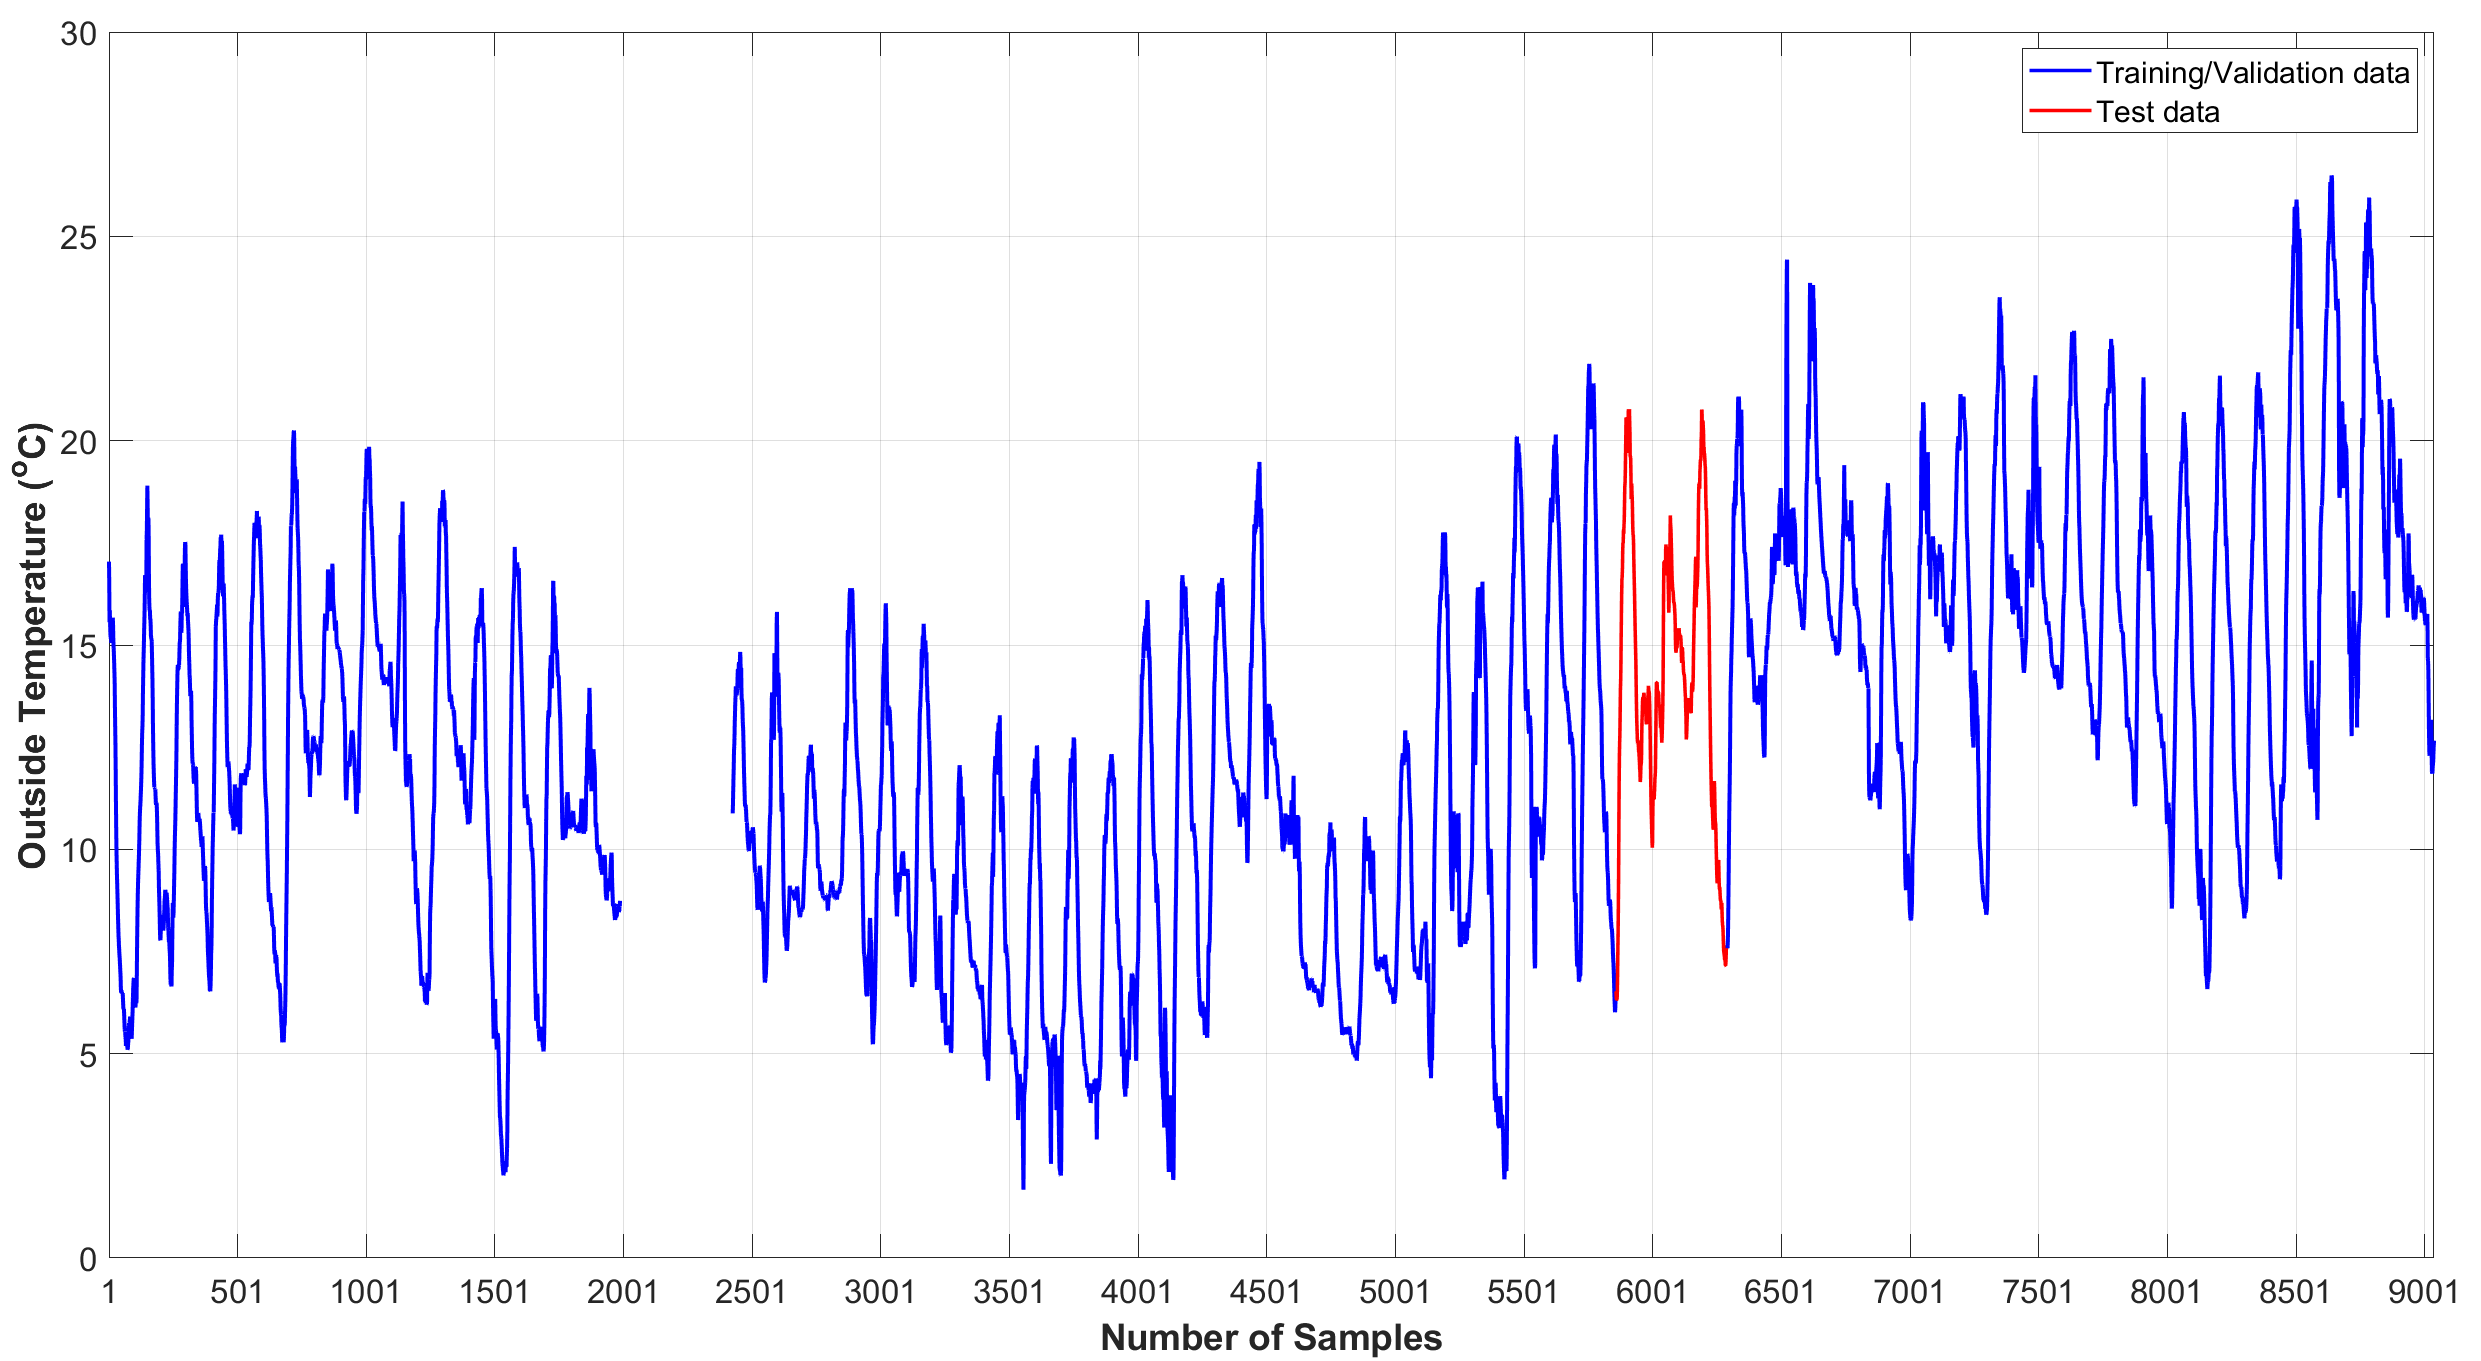
\includegraphics[scale=0.21]{Figures/NN_T_out.png}
            \caption*{\hspace{35pt}(α)}{}
        \end{minipage}
        \hfill
        \begin{minipage}[c]{0.48\textwidth}
            \centering
            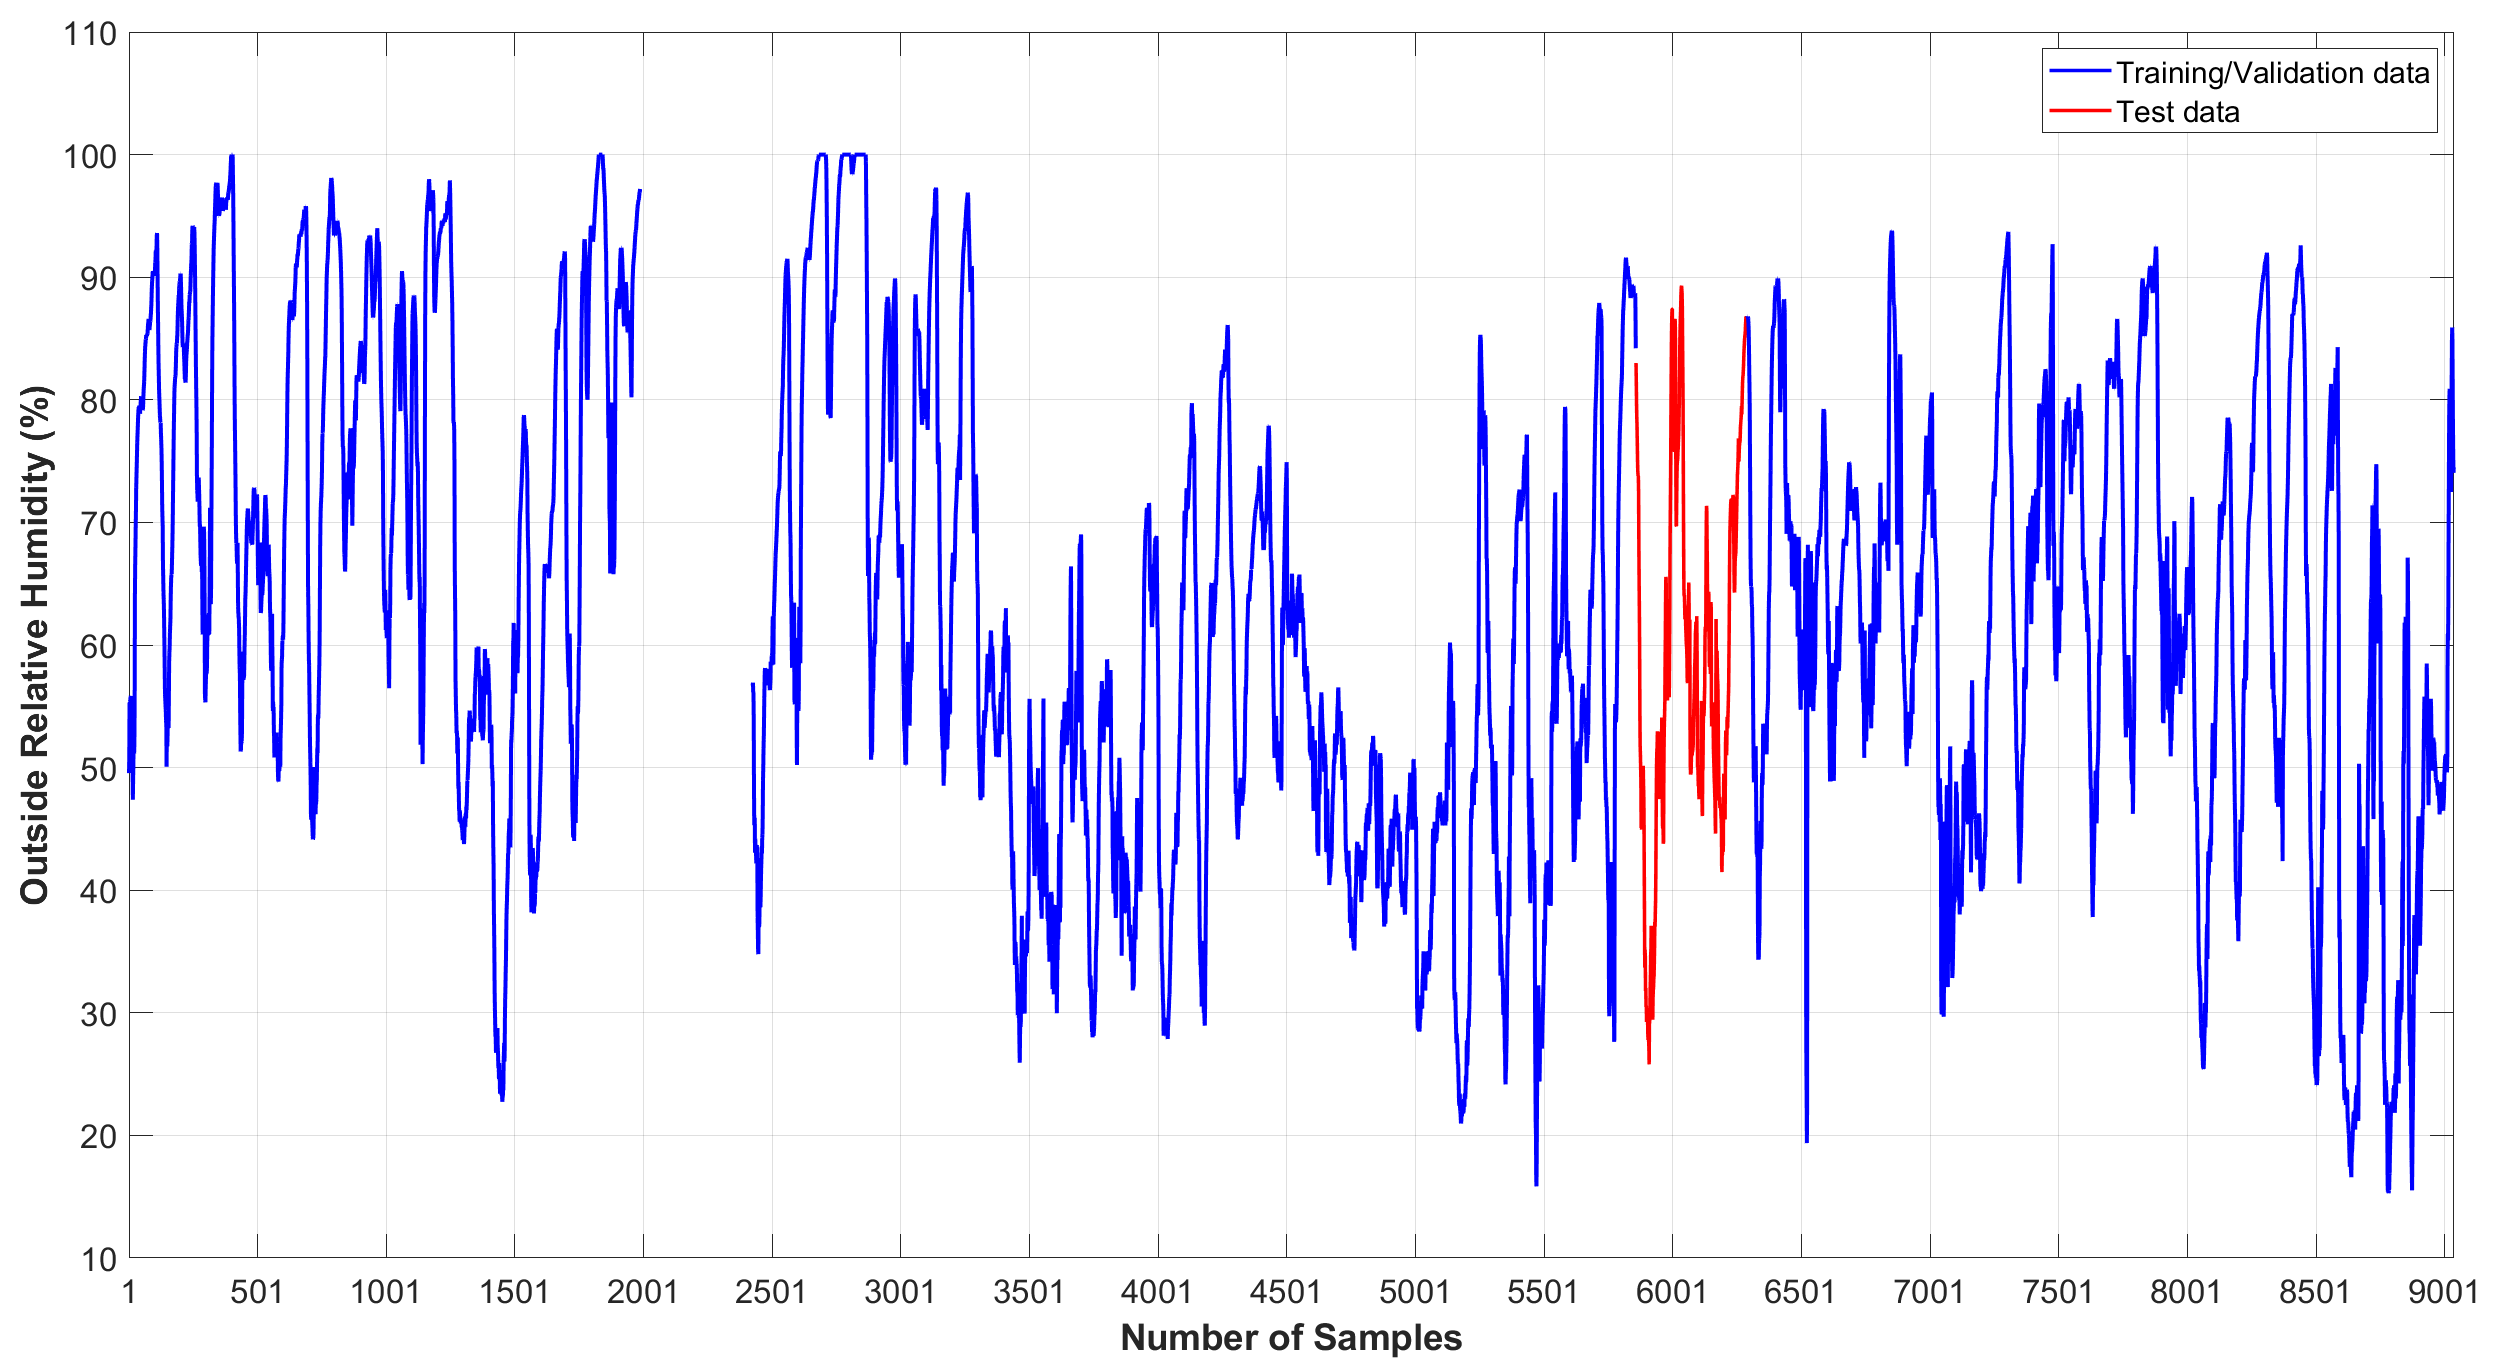
\includegraphics[scale=0.21]{Figures/NN_RH_out.png}
            \caption*{\hspace{35pt}(β)}{}
        \end{minipage}

        \medskip

        \begin{minipage}[c]{0.48\textwidth}
            \centering
            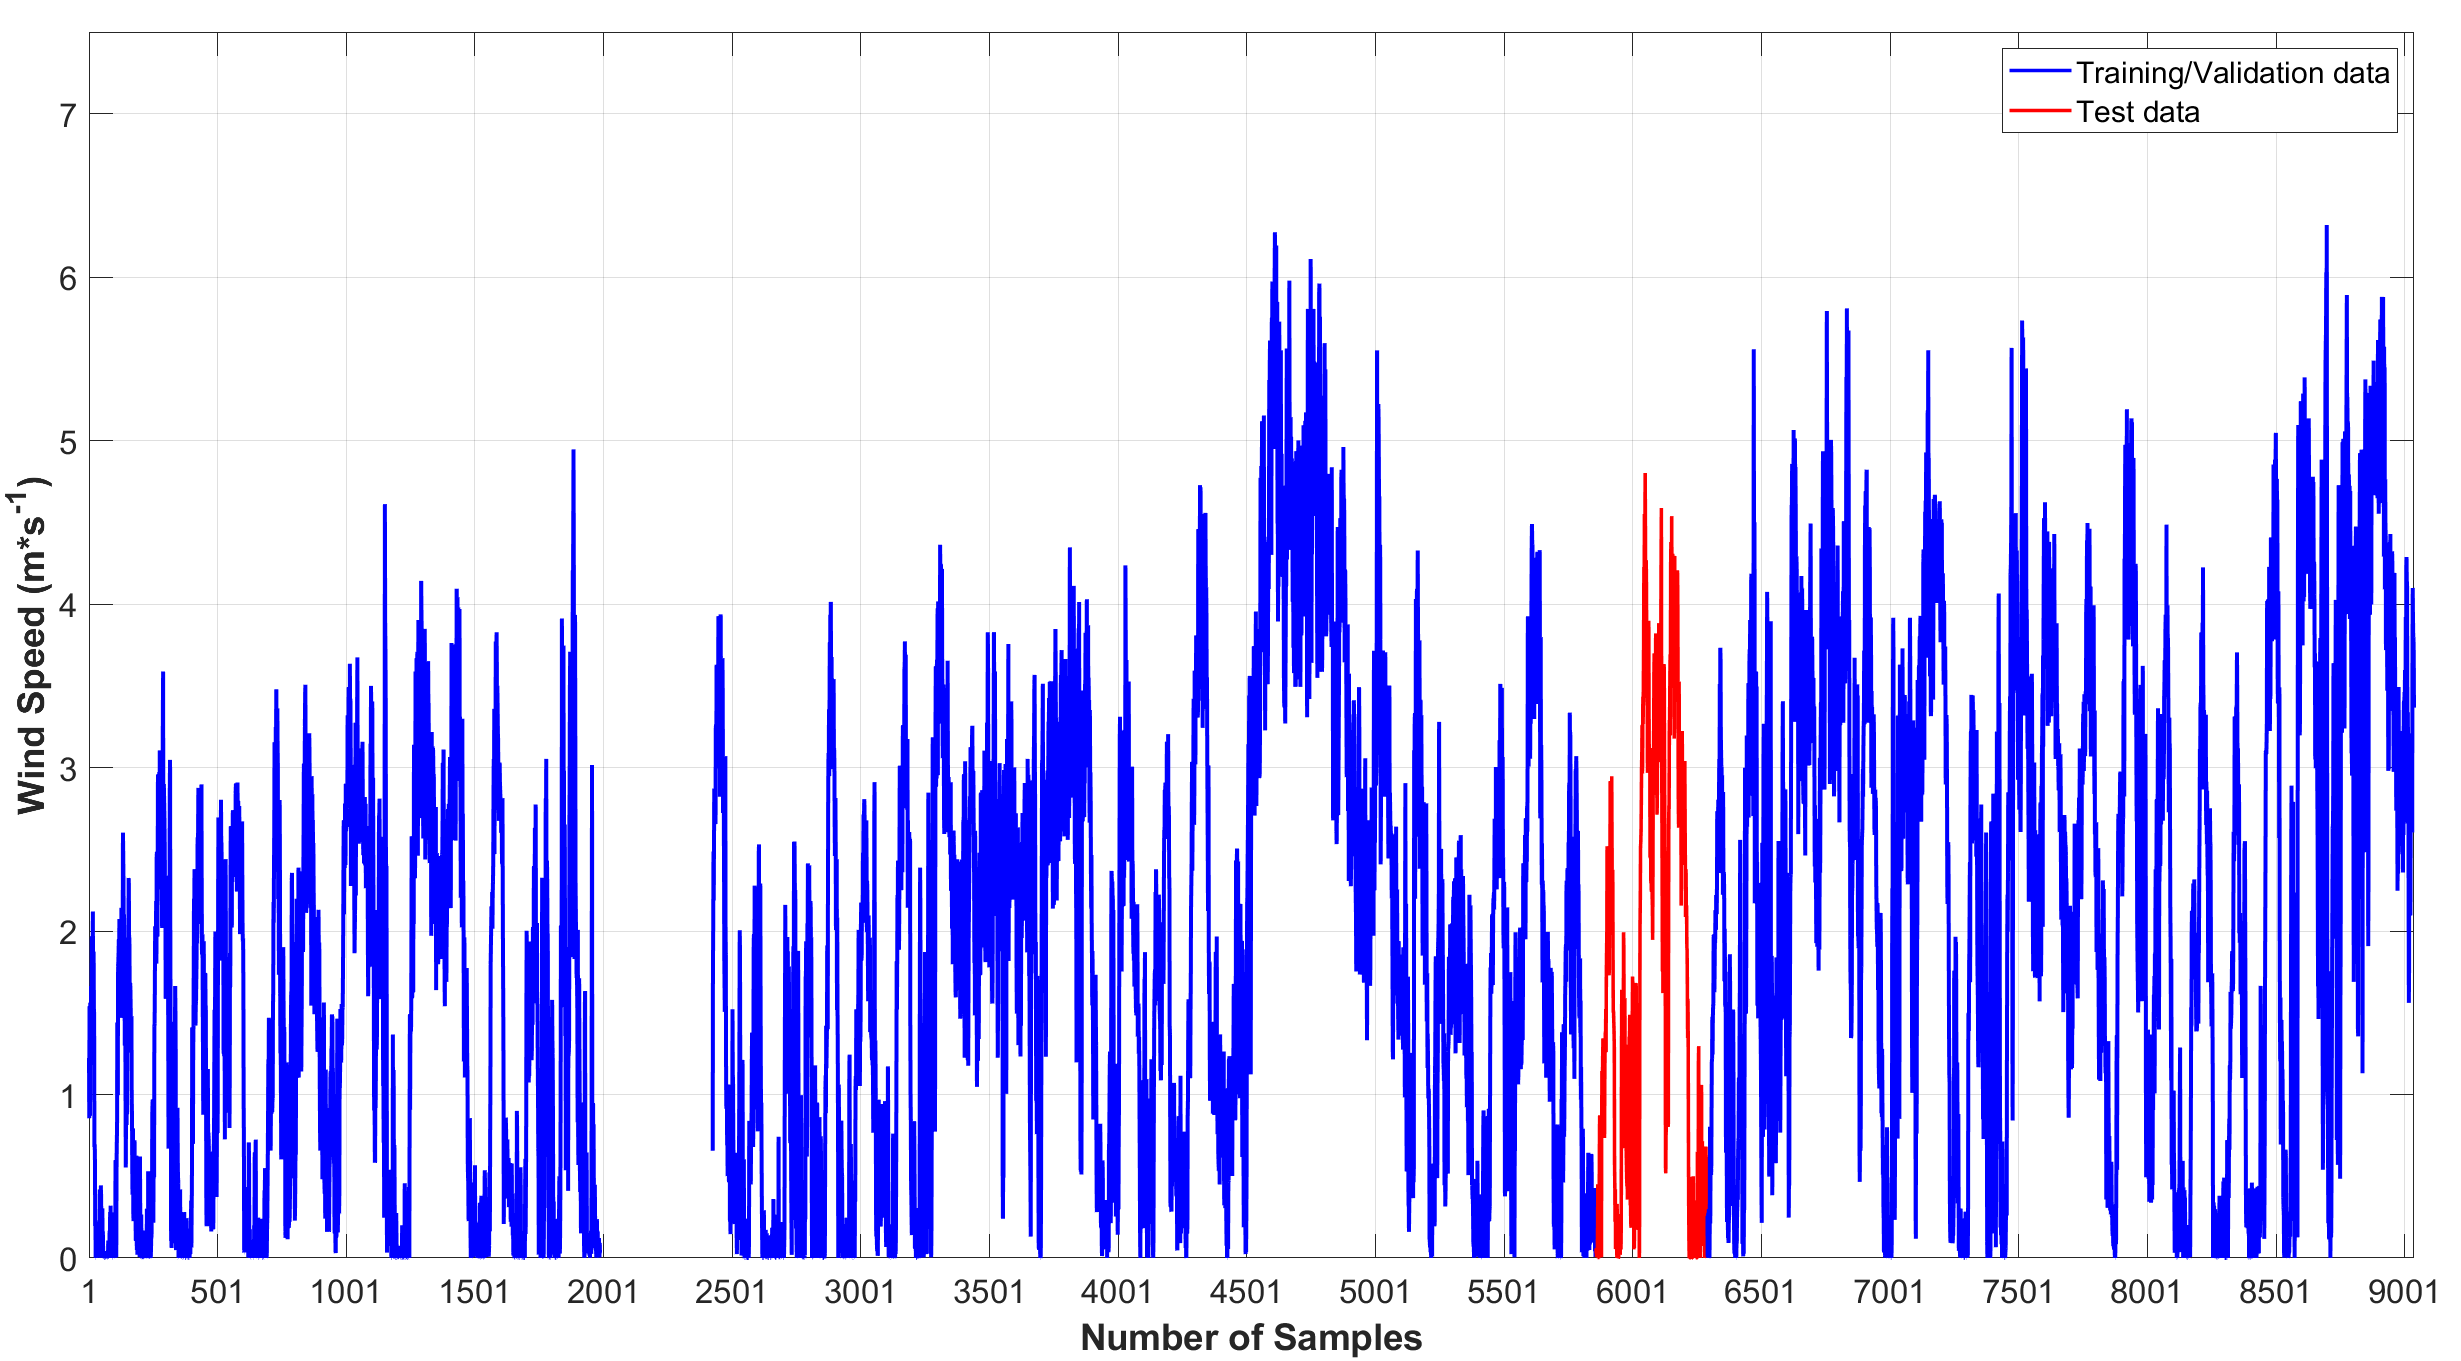
\includegraphics[scale=0.21]{Figures/NN_WS.png}
            \caption*{\hspace{35pt}(γ)}{}
        \end{minipage}
        \hfill
        \begin{minipage}[c]{0.48\textwidth}
            \centering
            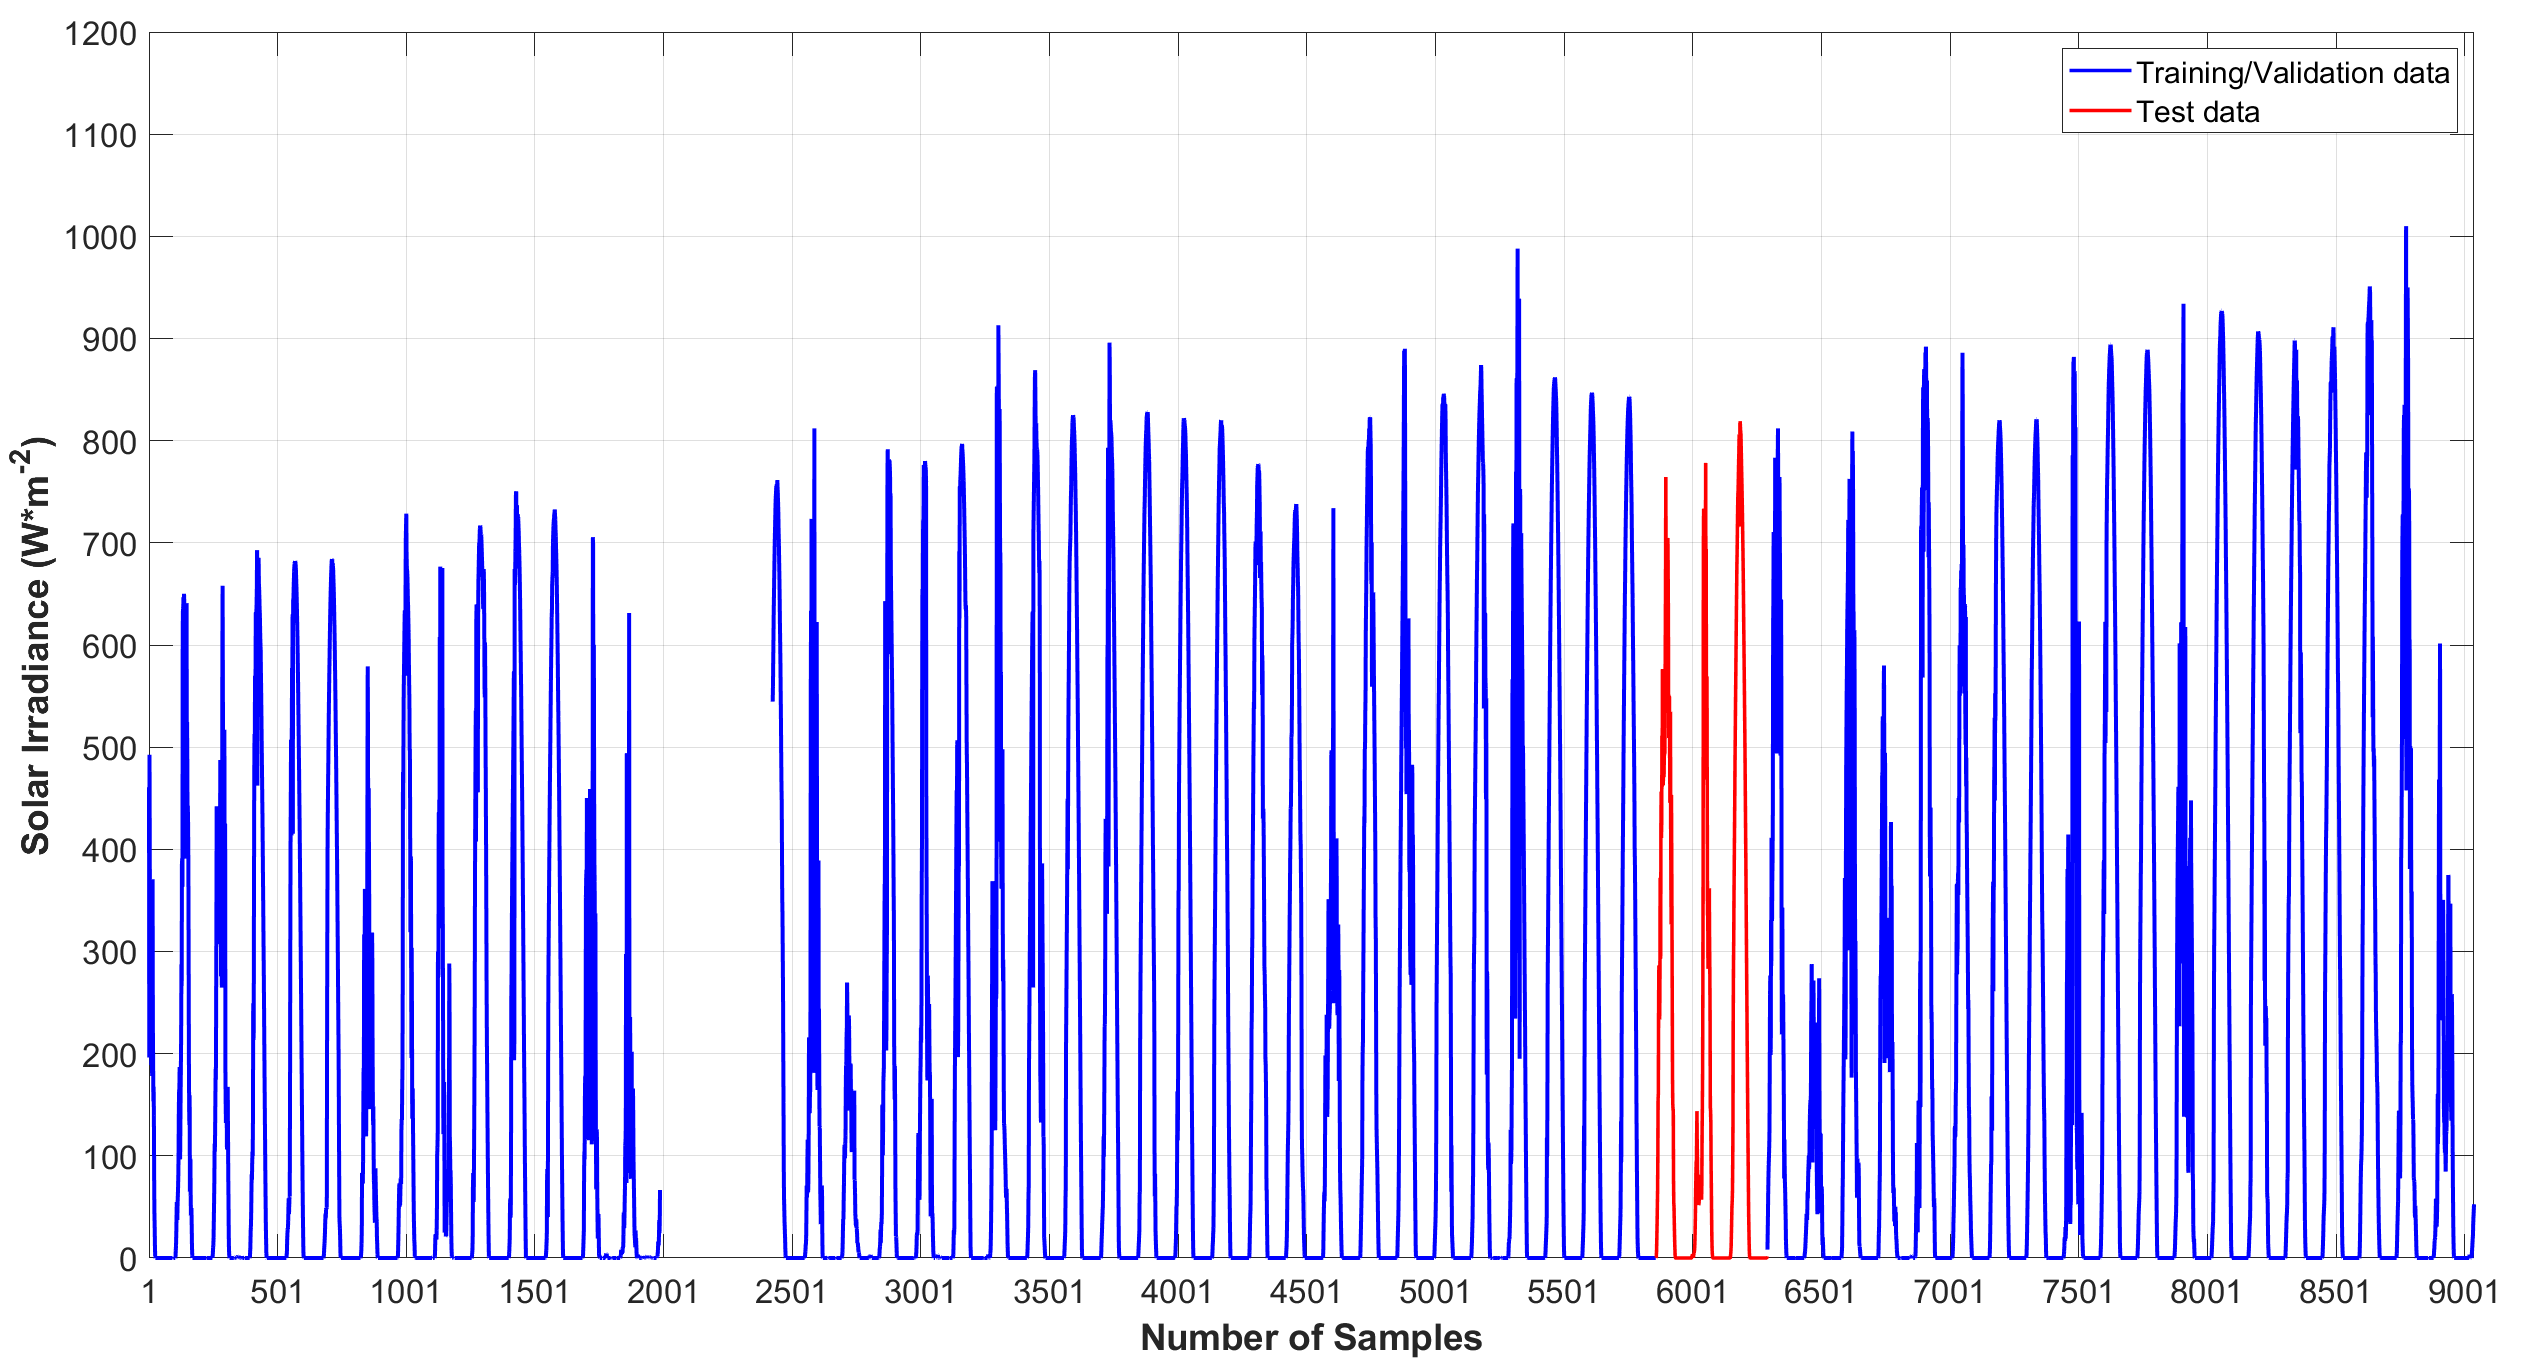
\includegraphics[scale=0.21]{Figures/NN_SR.png}
            \caption*{\hspace{35pt}(δ)}{}
        \end{minipage}

        \medskip

        \begin{minipage}[c]{0.48\textwidth}
            \centering
            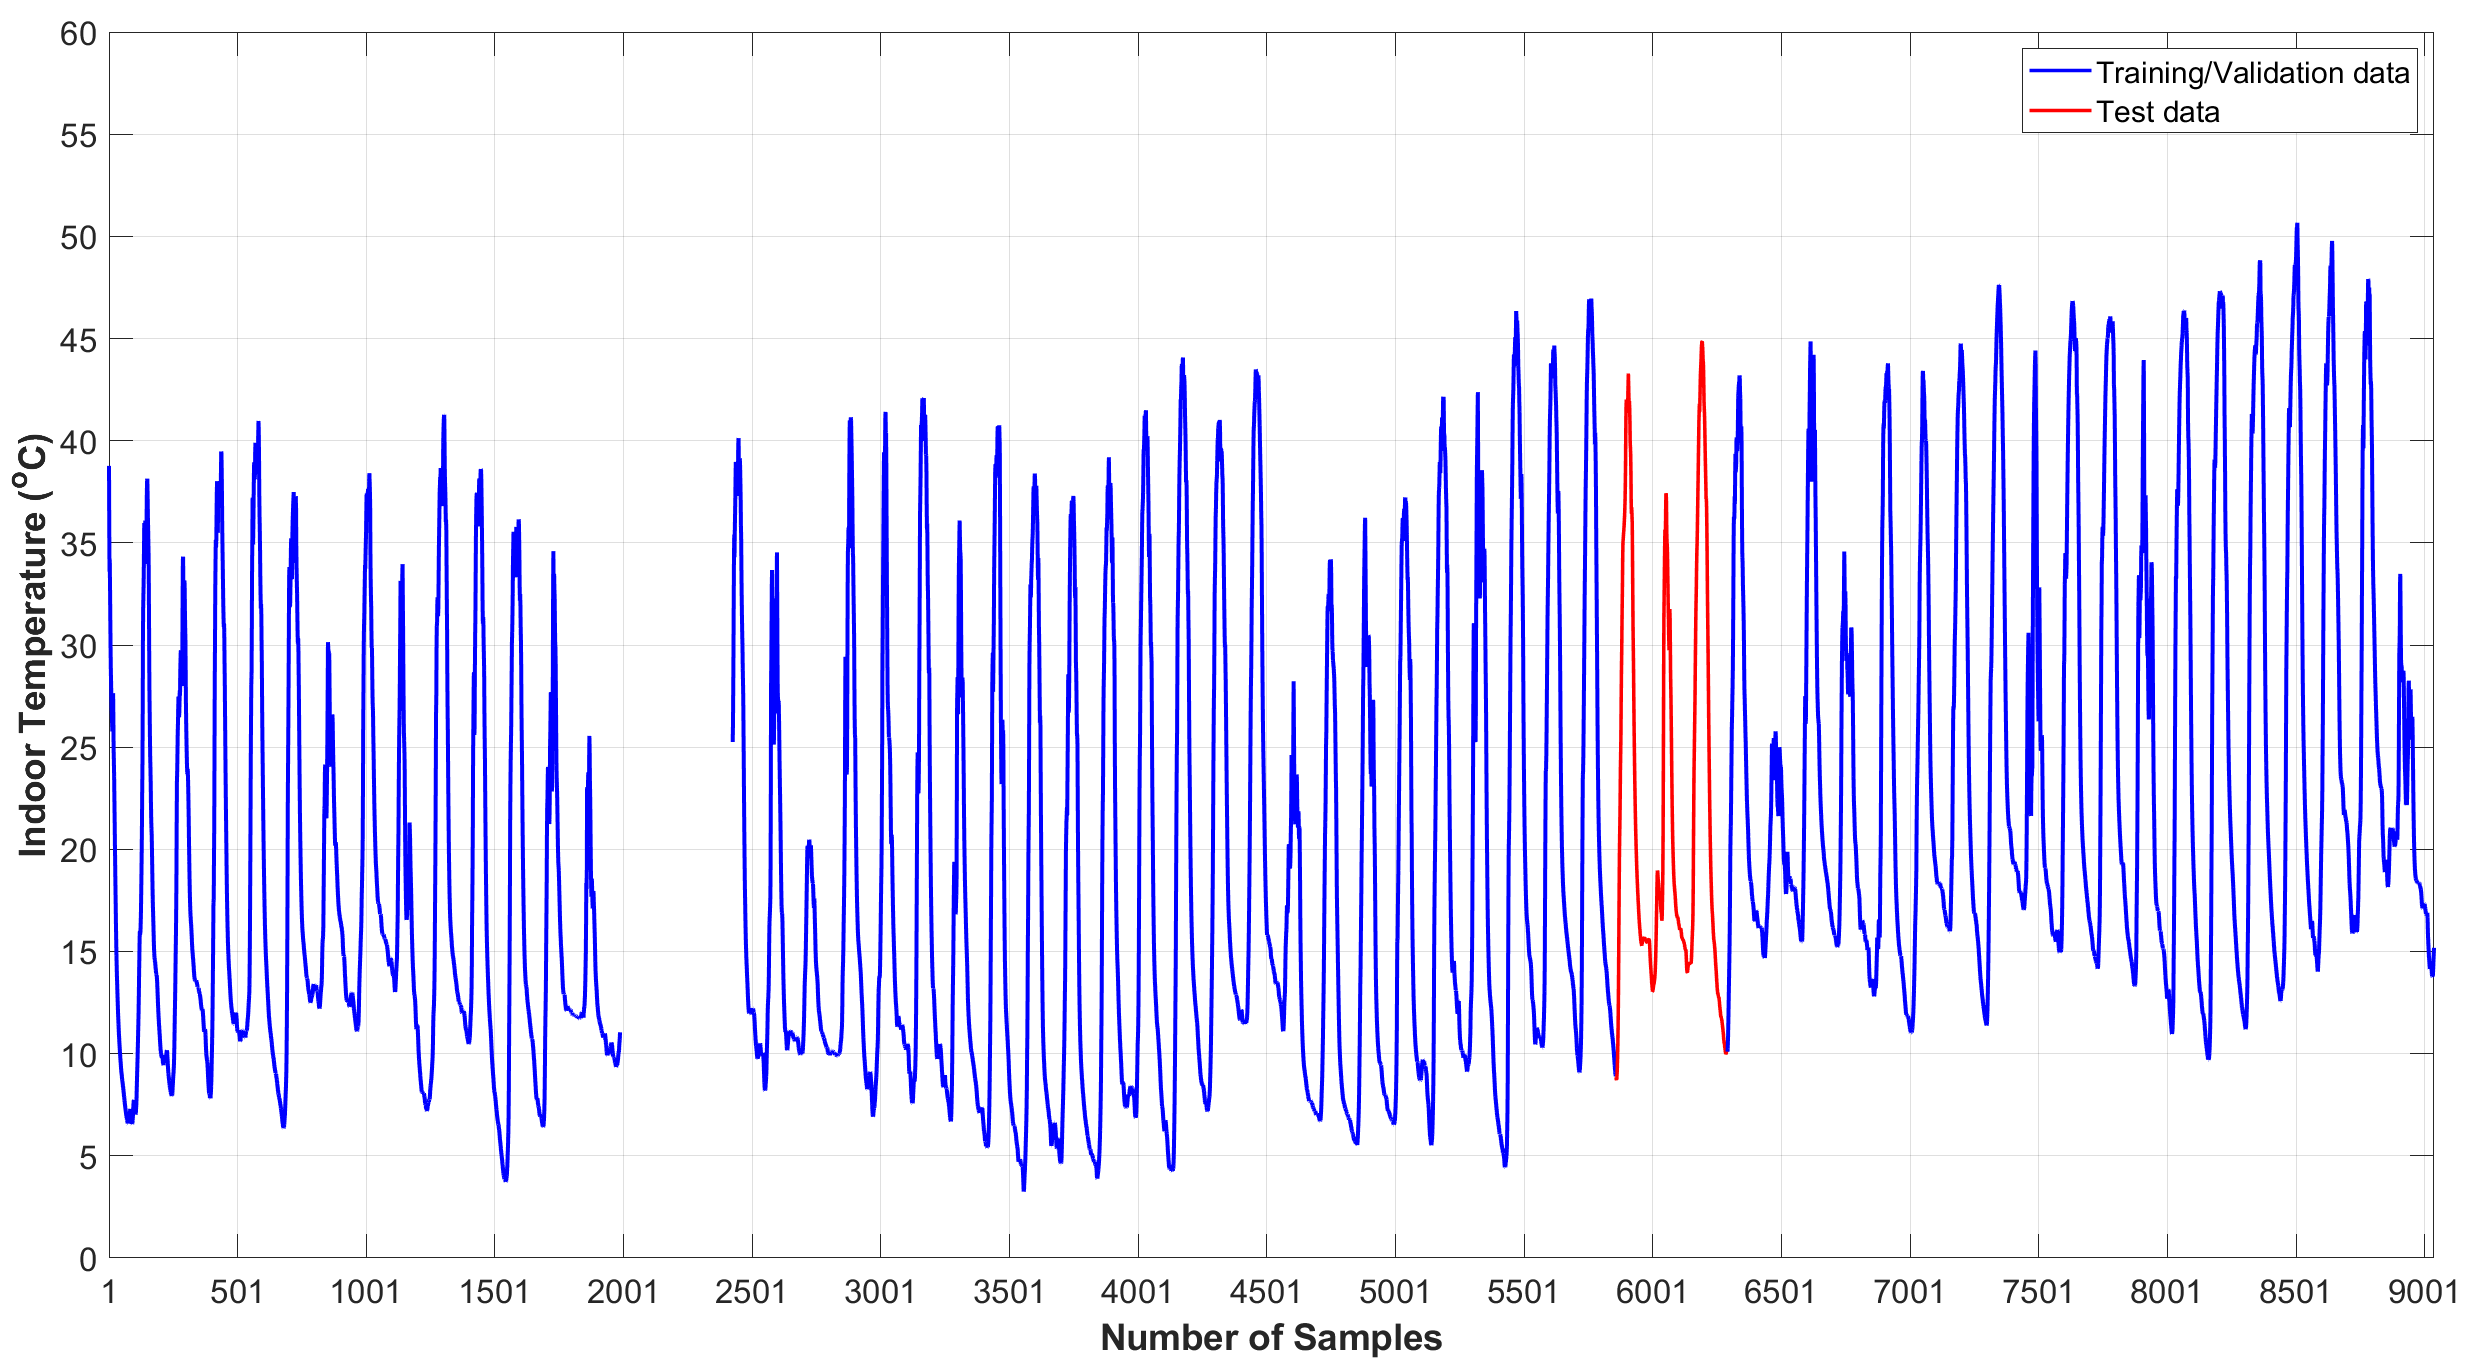
\includegraphics[scale=0.21]{Figures/NN_T_in.png}
            \caption*{\hspace{35pt}(ε)}{}
        \end{minipage}
        \hfill
        \begin{minipage}[c]{0.48\textwidth}
            \centering
            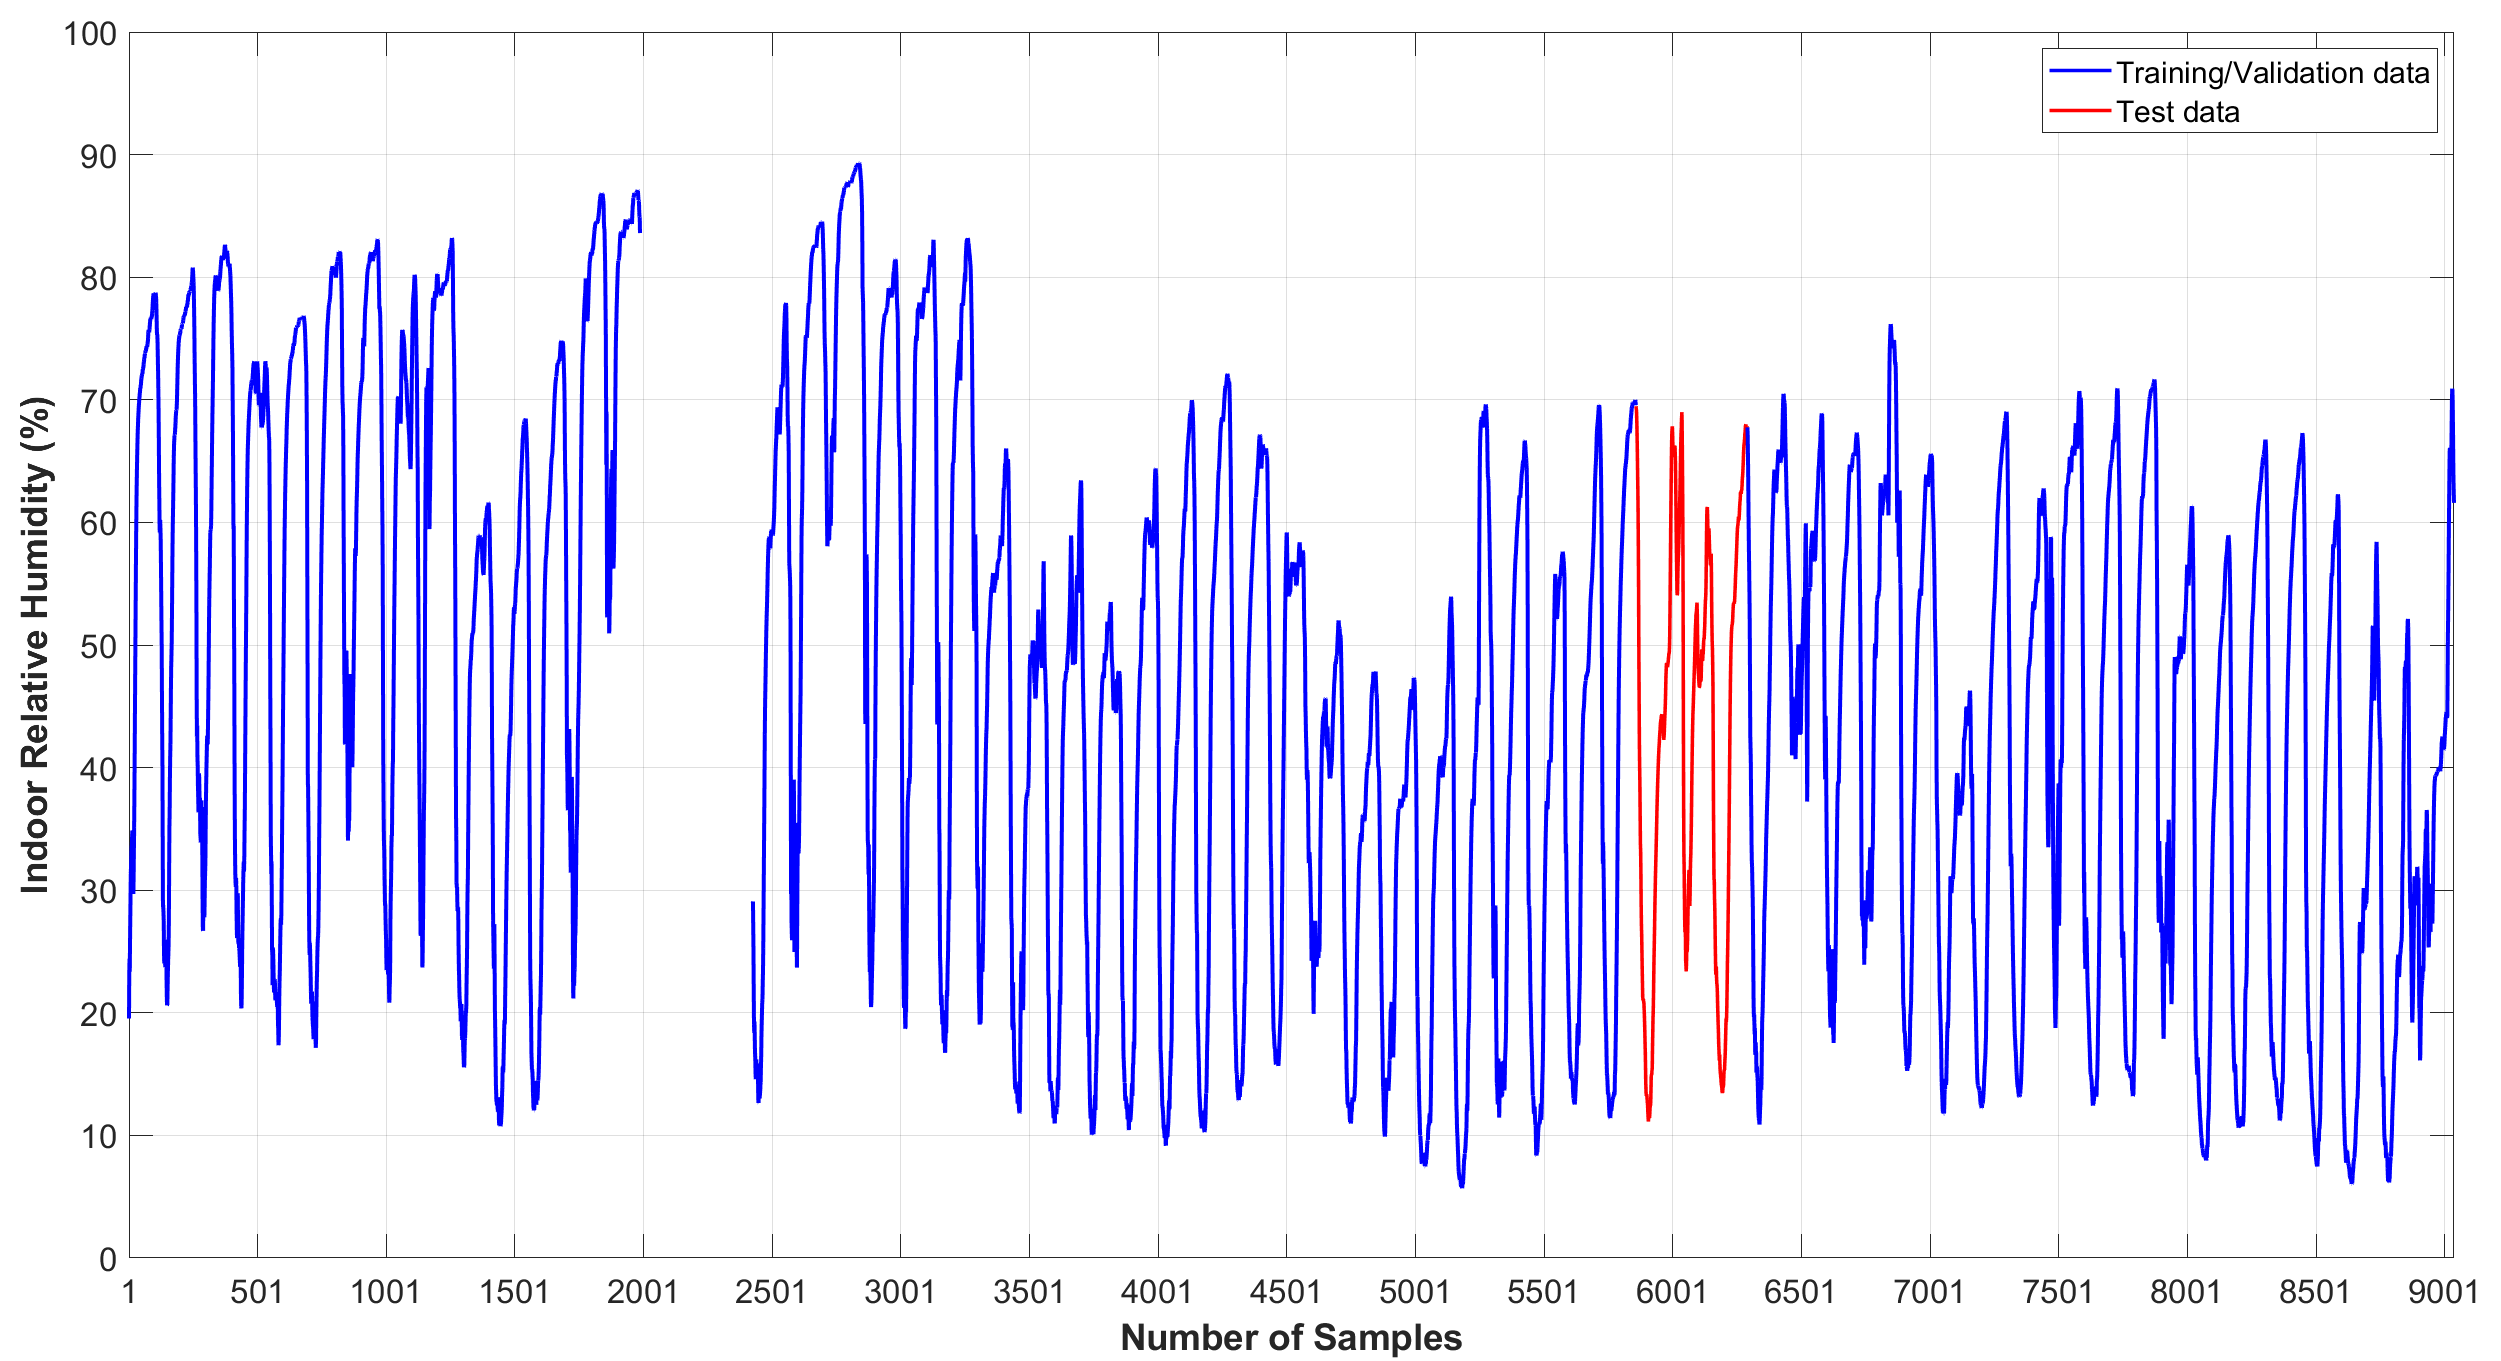
\includegraphics[scale=0.135]{Figures/NN_RH_in.png}
            \caption*{\hspace{35pt}(στ)}{}
        \end{minipage}
    \end{adjustwidth}
        
\caption{Δεδομένα εκπαίδευσης/επικύρωσης και δοκιμής για (α) την εξωτερική θερμοκρασία (β) την εξωτερική σχετική υγρασία 
(γ) την ταχύτητα του ανέμου (δ) την ηλιακή ακτινοβολία (ε) την εσωτερική θερμοκρασία (στ) την εσωτερική σχετική υγρασία.}
\label{fig_NN_data}
\end{figure}

\clearpage

Όπως φαίνεται στις παραπάνω εικόνες, οι μεταβλητές εισόδου δεν έχουν ούτε τις ίδιες μονάδες, ούτε τις ίδιες τάξεις 
μεγέθους. Έτσι, μεταβλητές με μεγαλύτερες τιμές θα συμβάλουν περισσότερο στο σφάλμα εξόδου, με αποτέλεσμα ο αλγόριθμος 
να δίνει μεγαλύτερο βάρος σε αυτές και μικρότερο σε μεταβλητές με μικρότερο εύρος τιμών \lcitep{neural_bib17}. Για 
αυτούς τους λόγους, είναι απαραίτητο να γίνει κανονικοποίηση των μεταβλητών σε ένα εύρος από 0 έως 1 ή από -1 έως 1, 
ανάλογα με τη συνάρτηση ενεργοποίησης (\english{Activation Function}) του νευρωνικού δικτύου. Σε αυτή τη μελέτη, οι 
τιμές των μεταβλητών εισόδου και εξόδου κανονικοποιήθηκαν σε ένα εύρος μεταξύ 0,001 και 0,999 σύμφωνα με την Εξίσωση 
\ref{eq_normalization}, όπου οι παράμετροι \english{r$_{max}$} και \english{r$_{min}$} ισούνται με 0,999 και 0,001 
αντίστοιχα. Η κανονικοποίηση ελάχιστου-μέγιστου (\english{min-max}) επιλέχθηκε επειδή είναι η πιο γρήγορη, η πιο εύκολη 
και η πιο ευέλικτη μέθοδος κανονικοποίησης, ενώ με την προσθήκη των παραμέτρων \english{r$_{max}$} και 
\english{r$_{min}$}, το εύρος κανονικοποίησης μπορεί να αλλάξει εύκολα ανάλογα με τις ανάγκες της κάθε συνάρτησης 
ενεργοποίησης, ορίζοντας το αντίστοιχο μέγιστο και ελάχιστο όριο του εύρους σε αυτές.

\begin{equation}
    \english{Z_i = (r_{max} - r_{min}) \left( \frac{X_i - X_{min}}{X_{max} - X_{min}} \right) + r_{min}}
    \label{eq_normalization}
\end{equation}

Στην Εξίσωση \ref{eq_normalization}, η μεταβλητή \english{$Z_i$} παρουσιάζει την κανονικοποιημένη τιμή της μεταβλητής 
\english{$X_i$}, οι μεταβλητές \english{$X_{max}$} και \english{$X_{min}$} παρουσιάζουν τη μέγιστη και ελάχιστη τιμή 
της μεταβλητής \english{$X$}, αντίστοιχα, ενώ οι παράμετροι \english{$r_{max}$} και \english{$r_{min}$} λαμβάνουν τις 
τιμές των επιθυμητών ορίων του εύ\-ρους κανονικοποίησης. Το συγκεκριμένο εύρος κανονικοποίησης επιλέχθηκε λόγω της χρήσης 
της λογιστικής σιγμοειδούς συνάρτησης ενεργοποίησης (\english{logistic sigmoid activation function}) στο κρυφό επίπεδο 
του νευρωνικού δικτύου. Η λογιστική σιγμοειδής συνάρτηση ενεργοποίησης παρουσιάζεται από την Εξίσωση 
\ref{eq_logistic_act_fcn} και λαμβάνει τιμές σε ένα εύρος από 0 έως 1, όπως φαίνεται στην Εικόνα \ref{fig_log_sigm}, 
ωστόσο, επιλέχθηκε να χρησιμοποιηθούν πιο στενά όρια λόγω της ύπαρξης πιθανών ασυνεχειών στα όρια του εύρους. Στο τέλος 
της διαδικασίας, οι τιμές κανονικοποιήθηκαν για να ολοκληρωθεί η σύγκριση μεταξύ των προβλέψεων και των παρατηρήσεων.

\begin{equation}
    f(x) = \frac{1}{1 + e^{-x}}
    \label{eq_logistic_act_fcn}
\end{equation}

\begin{figure}[ht]%
    \centering
    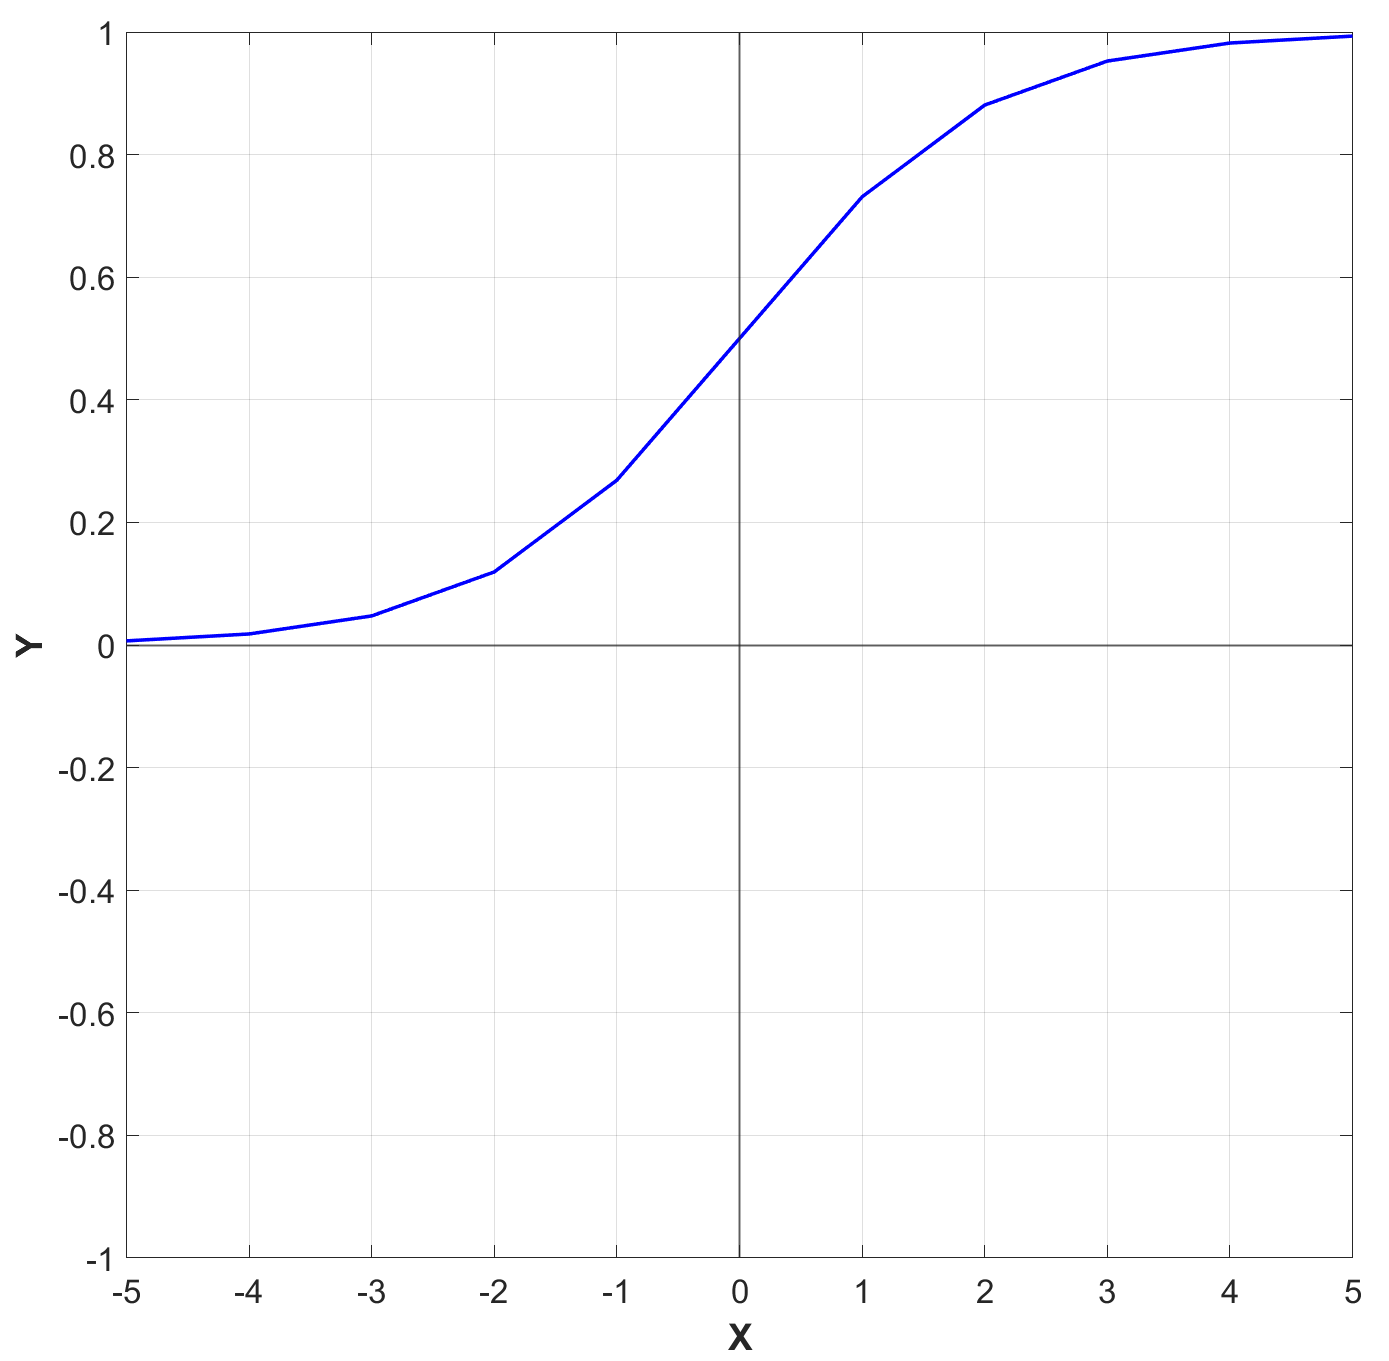
\includegraphics[scale=0.4]{Figures/log_act_fcn.png}
    \caption{Γραφική απεικόνιση της λογιστικής σιγμοειδούς συνάρτησης ενεργοποίησης.}
    \label{fig_log_sigm}
\end{figure}

Στη συνέχεια, και με την ολοκλήρωση της προεπεξεργασίας των δεδομένων, το σύνολο  των δεδομένων χωρίστηκε σε δύο 
διαφορετικά υποσύνολα. Το πρώτο, αποτελούμενο από 59 ημέρες και συνολικά 8161 δείγματα, διαμορφώθηκε τυχαία σε δύο 
υποσύνολα με το \SI{80}{\percent} των δειγμάτων να χρησιμοποιούνται για εκπαίδευση (\english{training}) και το υπόλοιπο 
\SI{20}{\percent} για την επικύρωση (\english{validation}) του μοντέλου. Οι εναπομένουσες 3 ημέρες (433 δείγματα) 
χρησιμοποιήθηκαν για να δοκιμαστεί (\english{testing}) το μοντέλο και να εξεταστεί η ικανότητα γενίκευσης των 
αποτελεσμάτων. Η χρονοσειρά διάρκειας 59 ημερών (δεδομένα εκπαίδευσης/επικύρωσης) αναπαρίσταται στις Εικόνες 
\ref{fig_NN_data}α, β, γ, δ, ε και στ με μπλε γραμμή, ενώ η χρονοσειρά διάρκειας 3 ημερών (δεδομένα δοκιμής) από 27 
Μαρτίου 2022 6:20 έως 30 Μαρτίου 2022 6:20 αναπαρίσταται με κόκκινη γραμμή.

Για τον έλεγχο των αποτελεσμάτων και της απόδοσης του μοντέλου, υπολογίστηκαν το Μέσο Απόλυτο Σφάλμα 
(\english{Mean Absolute Error – MAE}), η Τετραγωνική Ρίζα του Μέσου Τετραγωνικού Σφάλματος 
(\english{Root Mean Square Error – RMSE}) και ο Συντελεστής Προσδιορισμού (\english{Coefficient of Determination – R$^2$}) 
(Εξισώσεις \ref{eq_MAE}-\ref{eq_R_squared}), καθώς και το μέγιστο σφάλμα. Το μέγιστο σφάλμα αποτελεί ένα πολύ σημαντικό 
μέγεθος για ένα σύστημα υποστήριξης λήψης αποφάσεων, το οποίο θα ενεργοποιήσει τις διάφορες συσκευές διαχείρισης του 
μικροκλίματος του θερμοκηπίου βάσει των αποτελεσμάτων του μοντέλου.

\begin{equation}
    \english{MAE = \frac{1}{N} \sum_{i=1}^{N} \left| y_{pred.} - y_{obs.} \right|}
    \label{eq_MAE}
\end{equation}

\begin{equation}
    \english{RMSE = \sqrt{\frac{\sum_{i=1}^{N} \left( (y_{pred.} - y_{obs.})^2 \right)}{N}}}
    \label{eq_RMSE}
\end{equation}

\begin{equation}
    \english{R^2 = 1 - \frac{\sum_{i=1}^{N} \left( (y_{obs.} - y_{pred.})^2 \right)}{\sum_{i=1}^{N} \left( (y_{obs.} - \bar{y}_{obs.})^2 \right)}}
    \label{eq_R_squared}
\end{equation}

\subsection{Ανάπτυξη μοντέλου}\label{sub_NN_model}

Σε αυτή τη μελέτη, σχεδιάστηκε ένα νευρωνικό δίκτυο \english{MLP} με τρία διαφορετικά 
επίπεδα, το επίπεδο εισόδου, το κρυφό επίπεδο και το επίπεδο εξόδου. Το επίπεδο εισόδου αποτελείται από 10 κόμβους, 
έναν για κάθε ανεξάρτητη μεταβλητή, ενώ το επίπεδο εξόδου αποτελείται από 2 κόμβους, έναν για την εσωτερική θερμοκρασία 
και έναν για την εσωτερική σχετική υγρασία κατά την χρονική στιγμή \english{$t_0$}. Όσον αφορά τα ενδιάμεσα επίπεδα, επιλέχθηκε η 
προσθήκη ενός μόνο κρυφού επιπέδου, καθώς σύμφωνα με το θεώρημα του \english{Kolmogorov}, σε ένα \english{MLP} νευρωνικό 
δίκτυο ένα κρυφό επίπεδο με κατάλληλο αριθμό κόμβων μπορεί να δώσει αξιόπιστα αποτελέσματα για οποιαδήποτε διεργασία 
\lcitep{eisagwgi_NN_bib2,neural_bib18}.

Για την εύρεση της καλύτερης αρχιτεκτονικής του νευρωνικού δικτύου, του καλύτερου αλγορίθμου εκπαίδευσης, και των 
συναρτήσεων ενεργοποίησης χρησιμοποιήθηκε η μέθοδος δοκιμής και σφάλματος (\english{trial-and-error}). Για την εύρεση 
της καλύτερης αρχιτεκτονικής, ο αριθμός των κόμβων στο κρυφό επίπεδο άλλαζε κάθε φορά. Οι αλγόριθμοι εκπαίδευσης που 
δοκιμάστηκαν ήταν τρεις από τους πιο ευρέως χρησιμοποιούμενους αλγορίθμους, ο αλγόριθμος οπίσθιας τροφοδότησης 
\english{Levenberg–Marquardt}, ο αλγόριθμος οπίσθιας τροφοδότησης Μπαεσιανής κανονικοποίησης 
(\english{Bayesian regularization backpropagation}) και ο αλγόριθμος οπίσθιας τροφοδότησης \english{BFGS Quasi-Newton}. 
Παράλληλα, δοκιμάστηκαν τέσσερις διαφορετικές συναρτήσεις ενεργοποί\-ησης για το κρυφό επίπεδο, η λογιστική σιγμοειδής 
(\english{logistic sigmoid}), η υπερβολική εφαπτομένη σιγμοειδής (\english{hyperbolic tanget sigmoid}), η συνάρτηση 
ενεργοποίησης ακτινικής βάσης (\english{radial basis}) και η θετική γραμμική (\english{positive linear}) συνάρτηση 
ενεργοποίησης. Στον Πίνακα 2 παρουσιάζονται οι αντίστοιχες εντολές στη γλώσσα προγραμματισμού \english{MATLAB} για και 
τους αλγορίθμους εκπαίδευσης και για τις συναρτήσεις ενεργοποίησης.

\begin{table}[ht]
    \centering
    \caption{Κώδικας \english{MATLAB} για τους δοκιμασμένους αλγορίθμους εκπαίδευσης και συναρτήσεις ενεργοποίησης.}\label{tab_tr_alg_act_fnc} 
        \begin{tabular}{>{\centering\arraybackslash}m{7.5cm} >{\centering\arraybackslash}m{7.5cm}}
        \toprule
        \textbf{Όνομα} & \textbf{Κώδικας \english{MATLAB}} \\
        \midrule
        \multicolumn{2}{c}{\textbf{Αλγόριθμοι Εκπαίδευσης}} \\
        \midrule
        \english{Levenberg–Marquardt backpropagation} & \texttt{\english{trainlm}} \\
        \english{Bayesian Regularization backpropagation} & \texttt{\english{trainbr}} \\ 
        \english{BFGS Quasi Newton backpropagation} & \texttt{\english{trainfg}} \\
        \midrule
        \multicolumn{2}{c}{\textbf{Συναρτήσεις Ενεργοποίησης}} \\
        \midrule
        \english{Logistic Sigmoid} & \texttt{\english{logsig}} \\
        \english{Hyperbolic Tangent Sigmoid} & \texttt{\english{tansig}} \\ 
        \english{Radial Basis} & \texttt{\english{radbas}} \\ 
        \english{Positive Linear} & \texttt{\english{poslin}} \\ 
        \bottomrule
    \end{tabular}
\end{table}

Με βάση τα αποτελέσματα, ο αλγόριθμος εκπαίδευσης που χρησιμοποιήθηκε στο νευρωνικό δίκτυο ήταν ο αλγόριθμος οπίσθιας 
τροφοδότησης \english{Levenberg–Marquardt}, ένας αλγόριθμος βασισμένος στη μέθοδο του \english{Newton}. Ο αλγόριθμος 
εκπαίδευσης \english{LMBP} είναι μια πολύ αξιόπιστη και γρήγορη λύση για πολυστρωματικά νευρωνικά δίκτυα και τη 
βελτιστοποίηση του σφάλματος της συνάρτησης που αποτελείται από το άθροισμα των τετραγώνων των μη γραμμικών διεργασιών 
\lcitep{neural_bib19,neural_bib20}. Ως συναρτήσεις ενεργοποίησης για το κρυφό και το επίπεδο εξόδου χρησιμοποιήθηκαν 
η λογιστική σιγμοειδής και η γραμμική, αντίστοιχα. Τέλος, ως συνάρτηση απόδοσης χρησιμοποιήθηκε το μέσο τετραγωνικό 
σφάλμα (\english{MSE}). Στην Εικόνα \ref{fig_NN_struct} παρουσιάζεται μία γραφική αναπαράσταση του δημιουργημένου 
νευρωνικού δικτύου. Το μοντέλο αναπτύχθηκε και εκτελέστηκε σε γλώσσα προγραμματισμού \english{MATLAB}.

\begin{figure}[ht]%
    \centering
    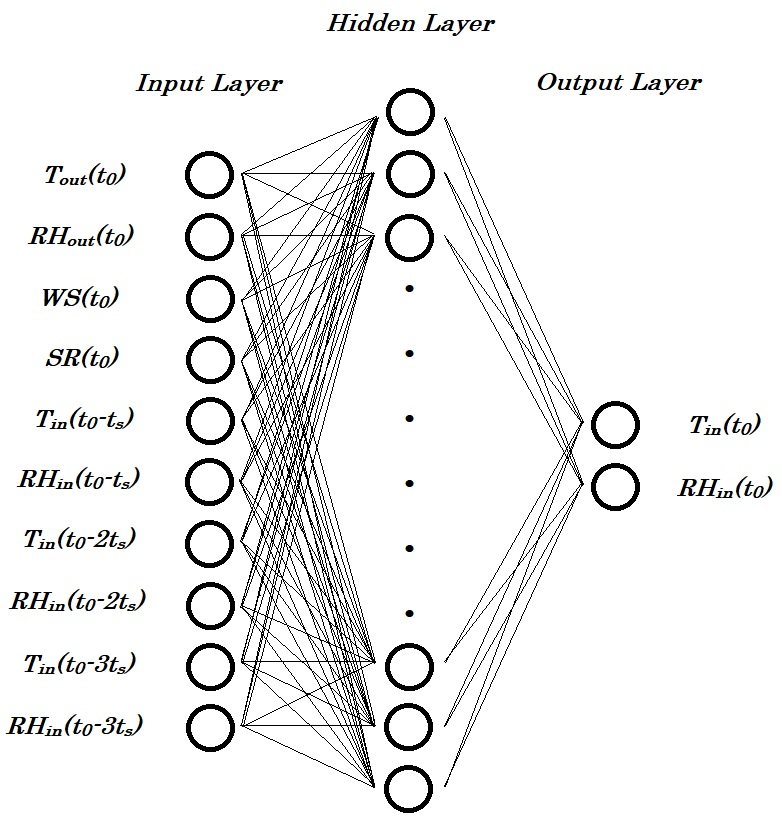
\includegraphics[scale=0.45]{Figures/NN_struct.jpg}
    \caption{Δομή του νευρωνικού δικτύου.}
    \label{fig_NN_struct}
\end{figure}

\subsection{Αποτελέσματα και συζήτηση}\label{sub_NN_results_disc}

Στο παρόν κεφάλαιο της μελέτης, χρησιμοποιήθηκε ένα Νευρωνικό Δίκτυο Πολυστρωματικής Αντίληψης για την πρόβλεψη της 
θερμοκρασίας και της σχετικής υγρασίας μέσα στο θερμοκήπιο. Προκειμένου να βρεθεί η βέλτιστη αρχιτεκτονική, και πιο 
συγκεκριμένα ο αριθμός των κόμβων στο κρυφό επίπεδο, το μοντέλο εκπαιδεύτηκε και δοκιμάστηκε για τα αντίστοιχα χρονικά 
διαστήματα που αναφέρονται στην Παράγραφο \ref{sub_data_method_NN}. Με το πέρας της εκτέλεσης της διαδικασίας για 
διαφορετικό αριθμό κρυφών κόμβων κάθε φορά (από 1 έως 20) και με βάση τους στατιστικούς δείκτες 
\english{MAE, RMSE, R$^2$}, και το μέγιστο σφάλμα, διαπιστώθηκε ότι η καλύτερη δομή του νευρωνικού δικτύου είναι 10-7-2, 
δίνοντας τα καλύτερα αποτελέσματα για τη δοκιμαστική περίοδο. Η δομή του μοντέλου που εξήχθη από το \english{MATLAB} παρουσιάζεται 
στην Εικόνα \ref{fig_NN_struct_matlab}, ενώ οι τιμές των προαναφερθέντων δεικτών παρουσιάζονται στον Πίνακα 
\ref{tab_result_values}, τόσο για τη θερμοκρασία όσο και για τη σχετική υγρασία. Σύμφωνα με τη συγκεκριμένη δομή του 
νευρωνικού δικτύου, δημιουργήθηκαν οι ακόλουθες γραφικές παραστάσεις, οι οποίες παρουσιάζουν συγκρίσεις μεταξύ των 
παρατηρούμενων και προβλεπόμενων τιμών των δύο μεταβλητών.

\begin{figure}[ht]%
    \centering
    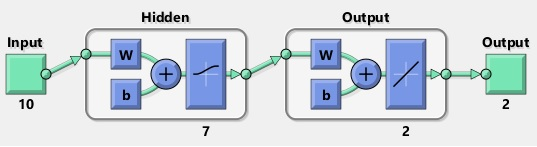
\includegraphics[scale=1.05]{Figures/NN_struct_matlab.jpg}
    \caption{Δομή μοντέλου ΤΝΔ στην \english{MATLAB}.}
    \label{fig_NN_struct_matlab}
\end{figure}

\begin{table}[ht]
    \centering
    \caption{Στατιστικοί δείκτες σύγκρισης μεταξύ παρατηρούμενων και προβλεπόμενων τιμών εσωτερικής θερμοκρασίας και σχετικής υγρασίας.}\label{tab_result_values} 
    \begin{tabular}{>{\centering\arraybackslash}m{4.85cm} >{\centering\arraybackslash}m{4.85cm} >{\centering\arraybackslash}m{4.85cm}}
        \toprule
        \textbf{Στατιστικοί Δείκτες} & \textbf{Θερμοκρασία} & \textbf{Σχετική Υγρασία} \\
        \midrule
        \english{MAE} & \SI{0,218}{\kelvin} & \SI{0,339}{\percent} \\
        \english{RMSE} & \SI{0,271}{\kelvin} & \SI{0,481}{\percent} \\ 
        \english{R$^2$} & \SI{0,999}{} & \SI{0,999}{} \\
        \english{MAX ERROR} & \SI{0,877}{\kelvin} & \SI{2,838}{\percent} \\
        \hline
        \end{tabular}
\end{table}

Η διαδικασία εκπαίδευσης του μοντέλου ολοκληρώθηκε μετά από 89 επαναλήψεις (\english{epochs}) (Εικόνα \ref{fig_NN_MSE}), 
όπου το μέσο τετραγωνικό σφάλμα επικύρωσης (\english{MSE}) παρουσίασε αύξηση για 6 φορές συνεχόμενα. Η συγκεκριμένη 
συνθήκη χρησιμοποιείται ως ένδειξη για την εύρεση του ελάχιστου \english{MSE}, και συνεπώς, του τερματισμού της 
διαδικασίας. Ο αριθμός των επαναλήψεων ήταν ίσος με 83, όπου το σφάλμα επικύρωσης παρουσίασε την ελάχιστη τιμή του ίση 
με περίπου $5.447 \cdot 10^{-5}$. Αυτή η τιμή προήλθε μέσω των κανονικοποιημένων μεταβλητών εισόδου και εξόδου και 
παρουσιάζει την καλύτερη απόδοση του μοντέλου.

\begin{figure}[ht]%
    \centering
    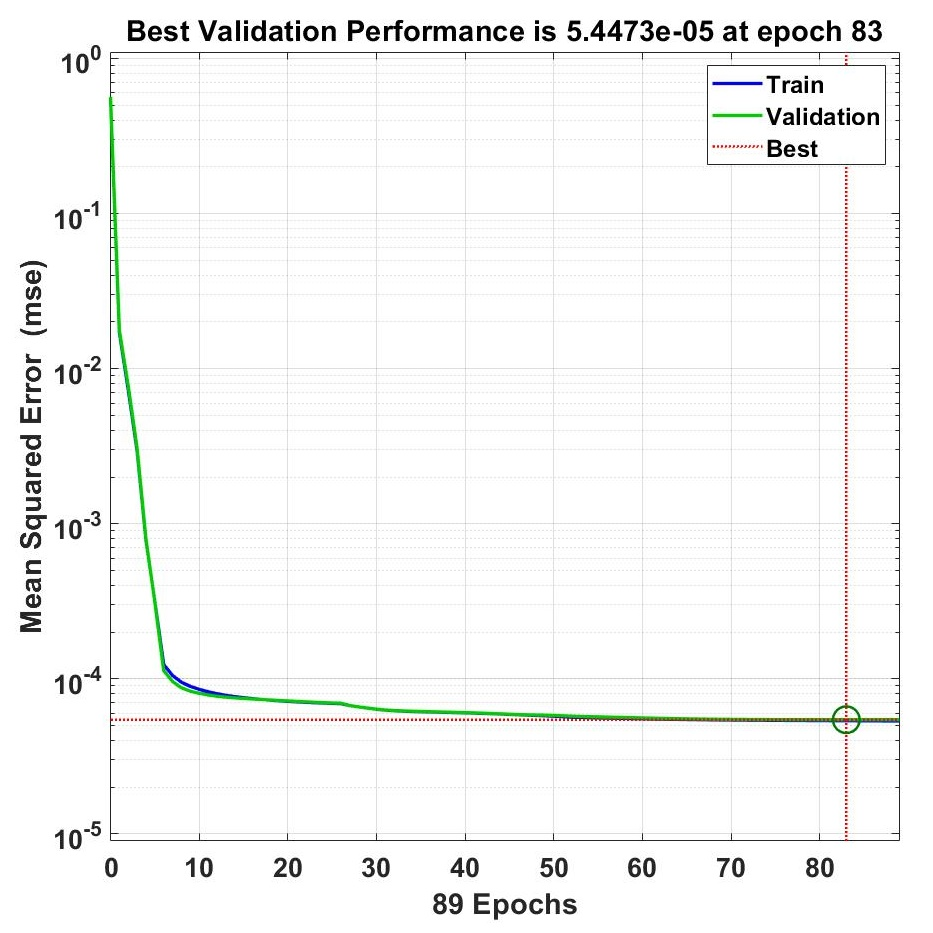
\includegraphics[scale=0.45]{Figures/NN_MSE.jpg}
    \caption{Σύγκλιση του μέσου τετραγώνου σφάλματος ως προς τις επαναλήψεις κατά την διαδικασία εκπαίδευσης και 
    επικύρωσης.}
    \label{fig_NN_MSE}
\end{figure}

Όσον αφορά τη θερμοκρασία εντός του θερμοκηπίου, με βάση τις τιμές των \english{MAE} και \english{RMSE}, τα οποία 
υπολογίστηκαν ίσα με \SI{0,218}{\kelvin} και \SI{0,271}{\kelvin}, αντίστοιχα, επιβεβαιώνεται η ικανότητα του μοντέλου 
να προβλέπει τη θερμοκρασία σε αρκετά ικανοποιητικό βαθμό. Ταυτόχρονα, με την διαφορά των τιμών των δύο αυτών δεικτών 
να είναι σχετικά μικρή, προκύπτει η απουσία μεγάλων σφαλμάτων από το μοντέλο. Η σχετική υγρασία κυμαίνεται στο ίδιο 
μήκος κύματος, με τις τιμές των \english{MAE} και \english{RMSE} να είναι πολύ μικρές και ίσες με \SI{0,339}{\percent} 
και \SI{0,48}{\percent}, αντίστοιχα. Οι συντελεστές προσδιορισμού είναι ίδιοι και για τις δύο παραμέτρους και ίσοι με 
0,999, υποδεικνύοντας την πολύ καλή απόδοση του μοντέλου. Τέλος, τα μέγιστα σφάλματα είναι ίσα με \SI{0,877}{\kelvin} 
και \SI{2,838}{\percent} για την θερμοκρασία και την σχετική υγρασία, αντίστοιχα.

Στις Εικόνες \ref{fig_NN_T_in_pred} και \ref{fig_NN_T_in_errors} παρουσιάζονται οι χρονοσειρές των προβλεπόμενων και 
παρατηρούμενων τιμών της θερμοκρασίας για τις 3 ημέρες που χρησιμοποιήθηκαν για την δοκιμή του μοντέλου, καθώς και τα 
αντίστοιχα σφάλματα μεταξύ των τιμών. Όπως φαίνεται από την Εικόνα \ref{fig_NN_T_in_pred}, το μοντέλο έχει προβλέψει τη 
θερμοκρασία σε μεγάλο βαθμό, με τα μεγαλύτερα σφάλματα να εμφανίζονται κατά τις ώρες της ημέρας, όταν δηλαδή η 
θερμοκρασία παρουσιάζει υψηλές τιμές, αλλά και απότομες αλλαγές (Εικόνα \ref{fig_NN_T_in_errors}). Μείωση των 
συγκεκριμένων σφαλμάτων έχει την δυνατότητα να γίνει προσθέτοντας μεγαλύτερο αριθμό δειγμάτων κατά την εκπαίδευση του 
μοντέλου. Στην Εικόνα \ref{fig_NN_RH_in_pred} και στην περίπτωση της σχετικής υγρασίας, παρουσιάζεται ξανά υψηλή 
προβλεψιμότητα του μοντέλου, με τις δύο καμπύλες να είναι σχεδόν ταυτόσημες. Ωστόσο, σύμφωνα με την Εικόνα 
\ref{fig_NN_RH_in_errors} και αντίθετα με την περίπτωση της θερμοκρασίας, τα σφάλματα δεν φαίνεται να ακολουθούν ένα 
σταθερό μοτίβο.

\begin{figure}[ht]%
    \centering
    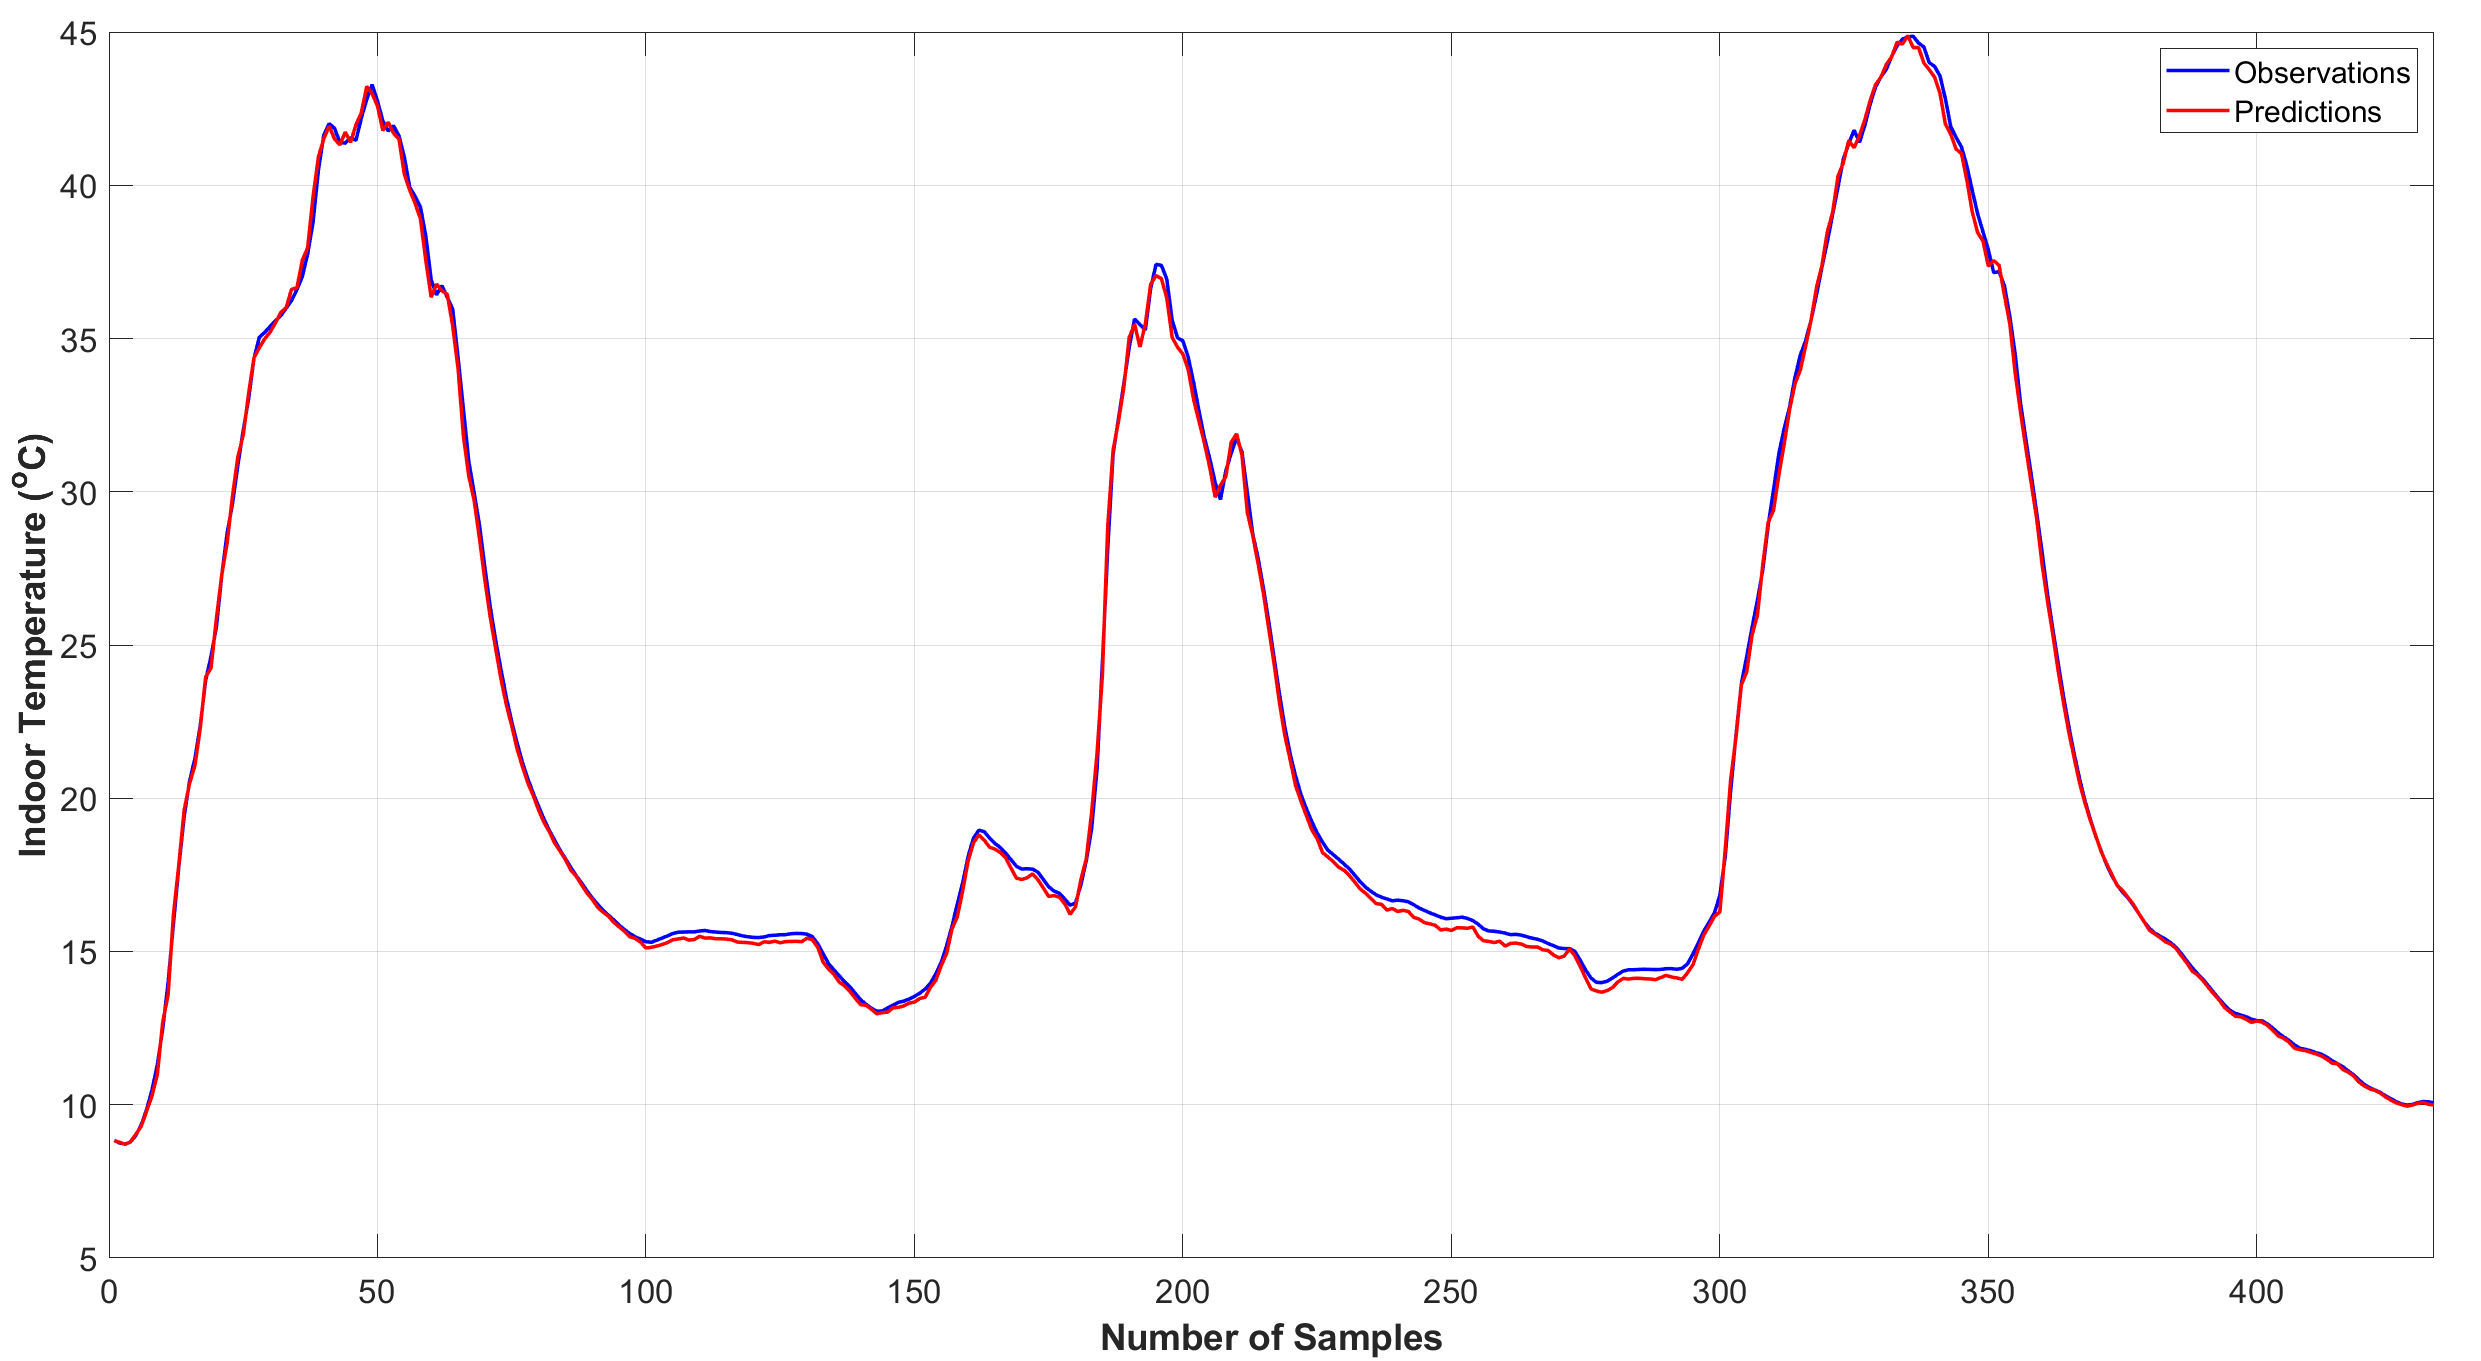
\includegraphics[width=0.9\textwidth]{Figures/NN_T_in_pred.png}
    \caption{Σύγκριση μεταξύ προβλεπόμενων τιμών και παρατηρήσεων για την θερμοκρασία εντός του θερμοκηπίου για την 
    περίοδο δοκιμής και δομής νευρωνικού δικτύου 10-7-2.}
    \label{fig_NN_T_in_pred}
\end{figure}

\begin{figure}[ht]%
    \centering
    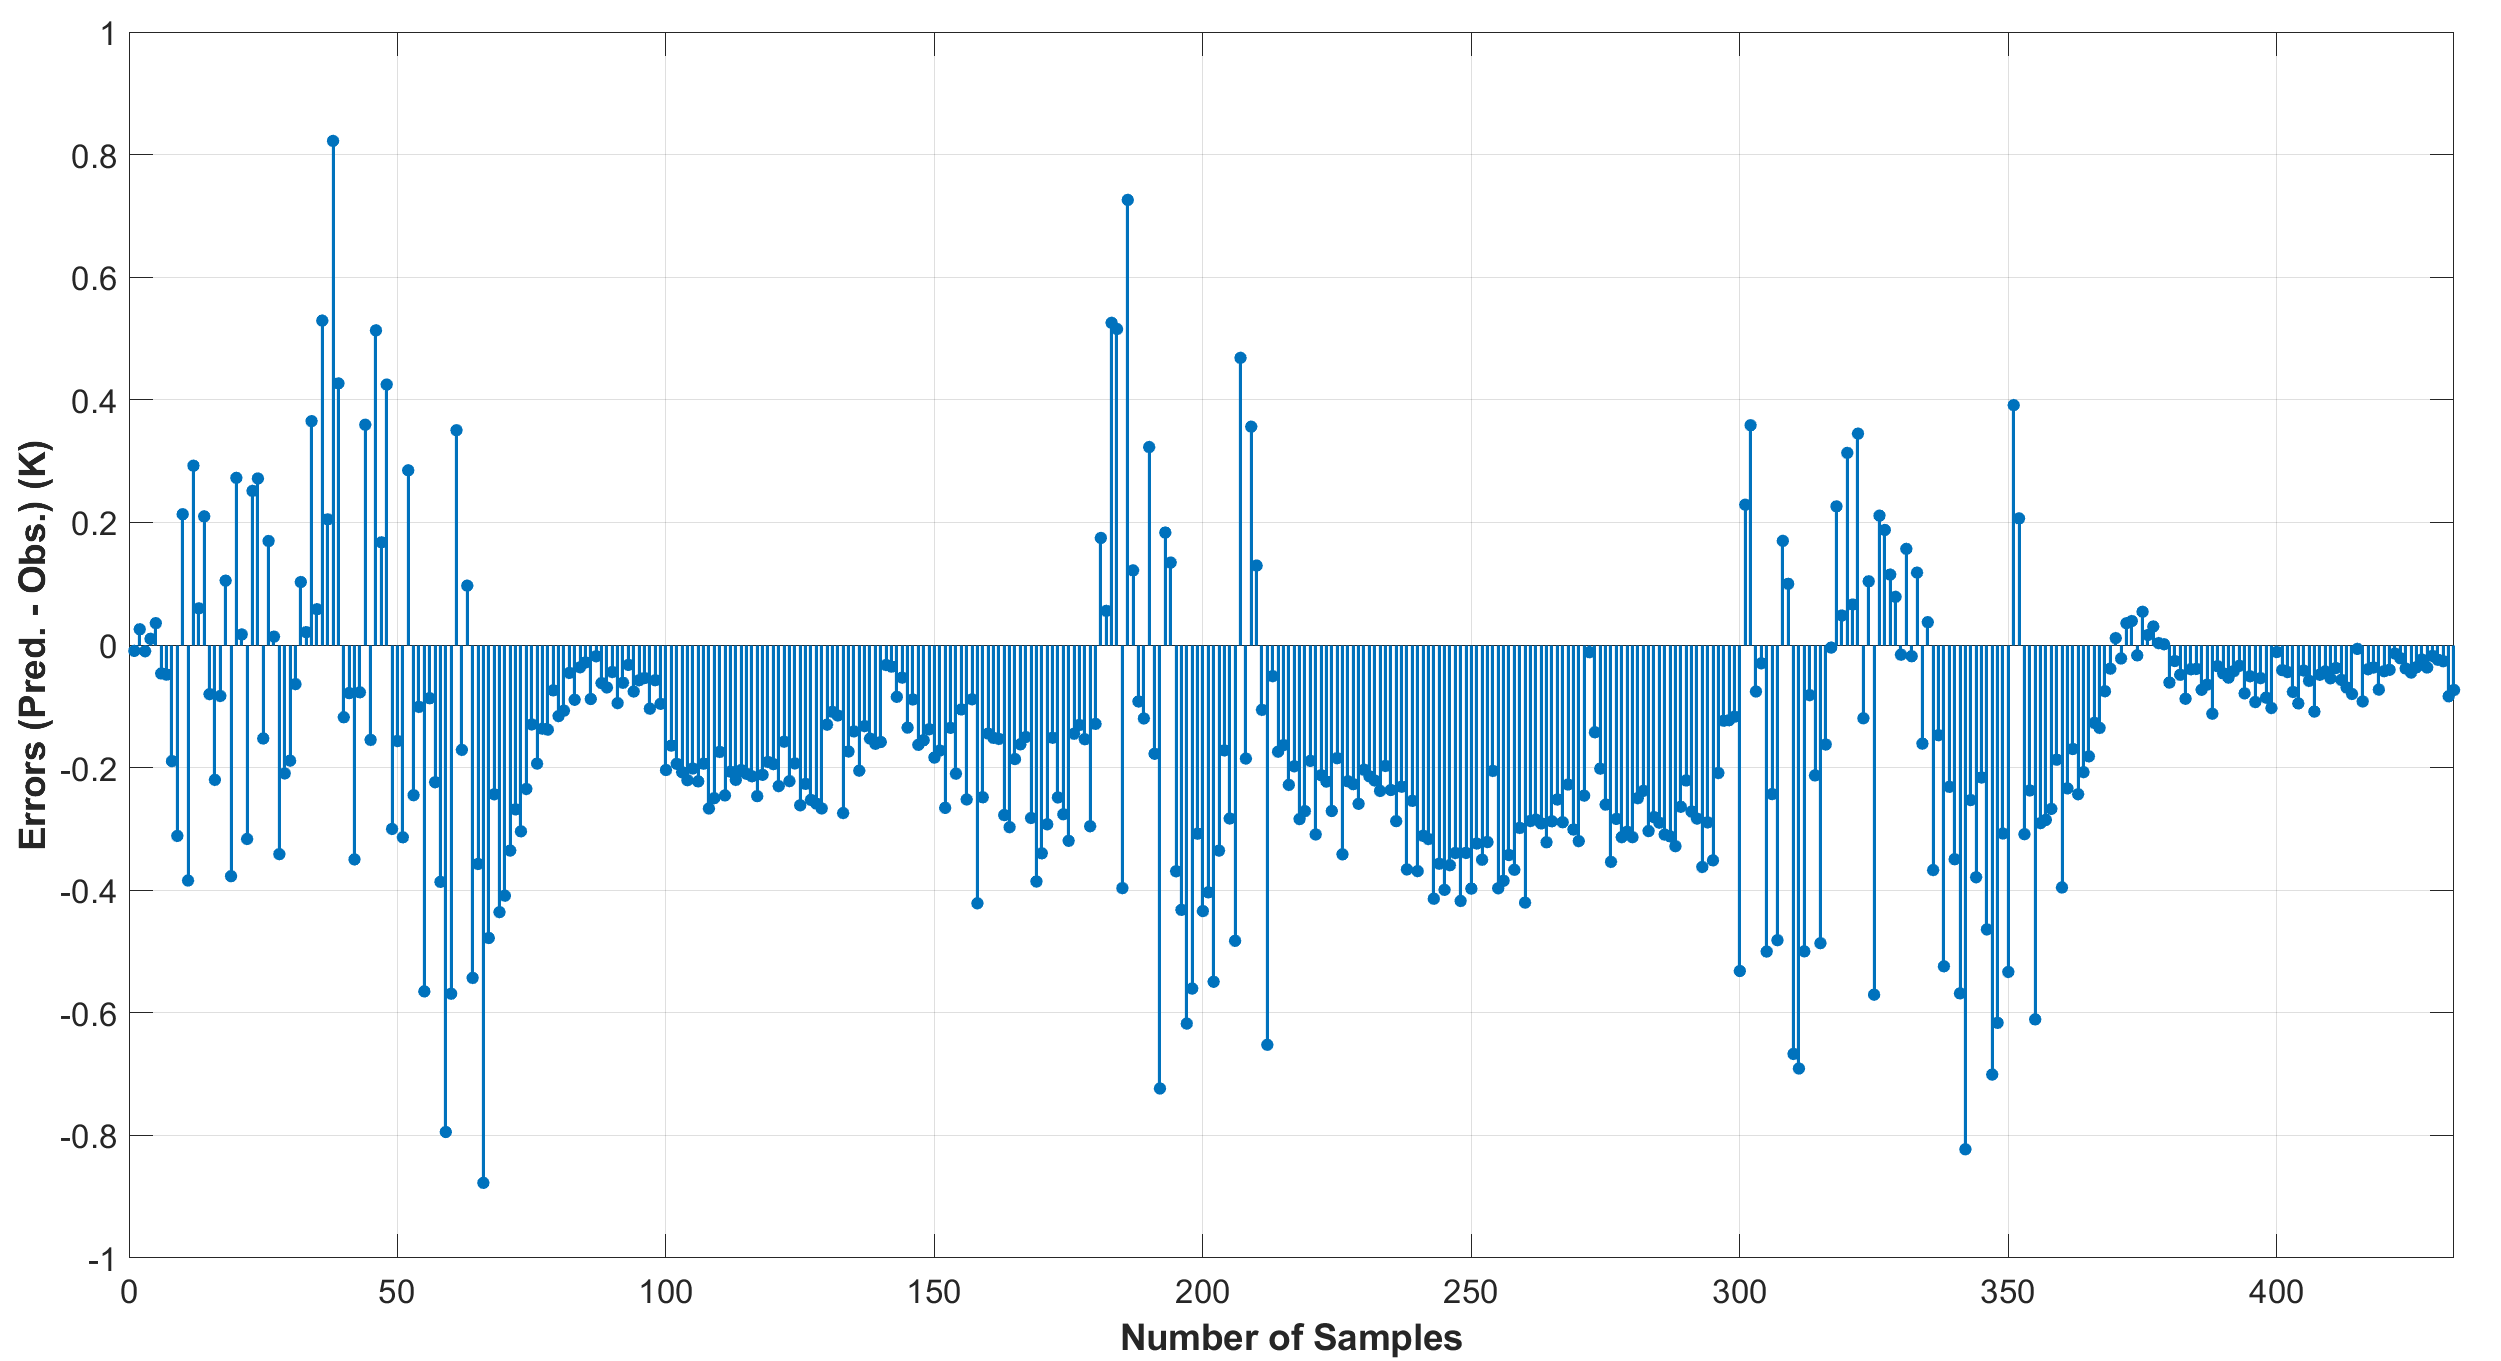
\includegraphics[width=0.9\textwidth]{Figures/NN_T_in_errors.png}
    \caption{Σφάλματα μεταξύ προβλεπόμενων τιμών και παρατηρήσεων για την θερμοκρασία εντός του θερμοκηπίου για την 
    περίοδο δοκιμής και δομής νευρωνικού δικτύου 10-7-2.}
    \label{fig_NN_T_in_errors}
\end{figure}

\begin{figure}[ht]%
    \centering
    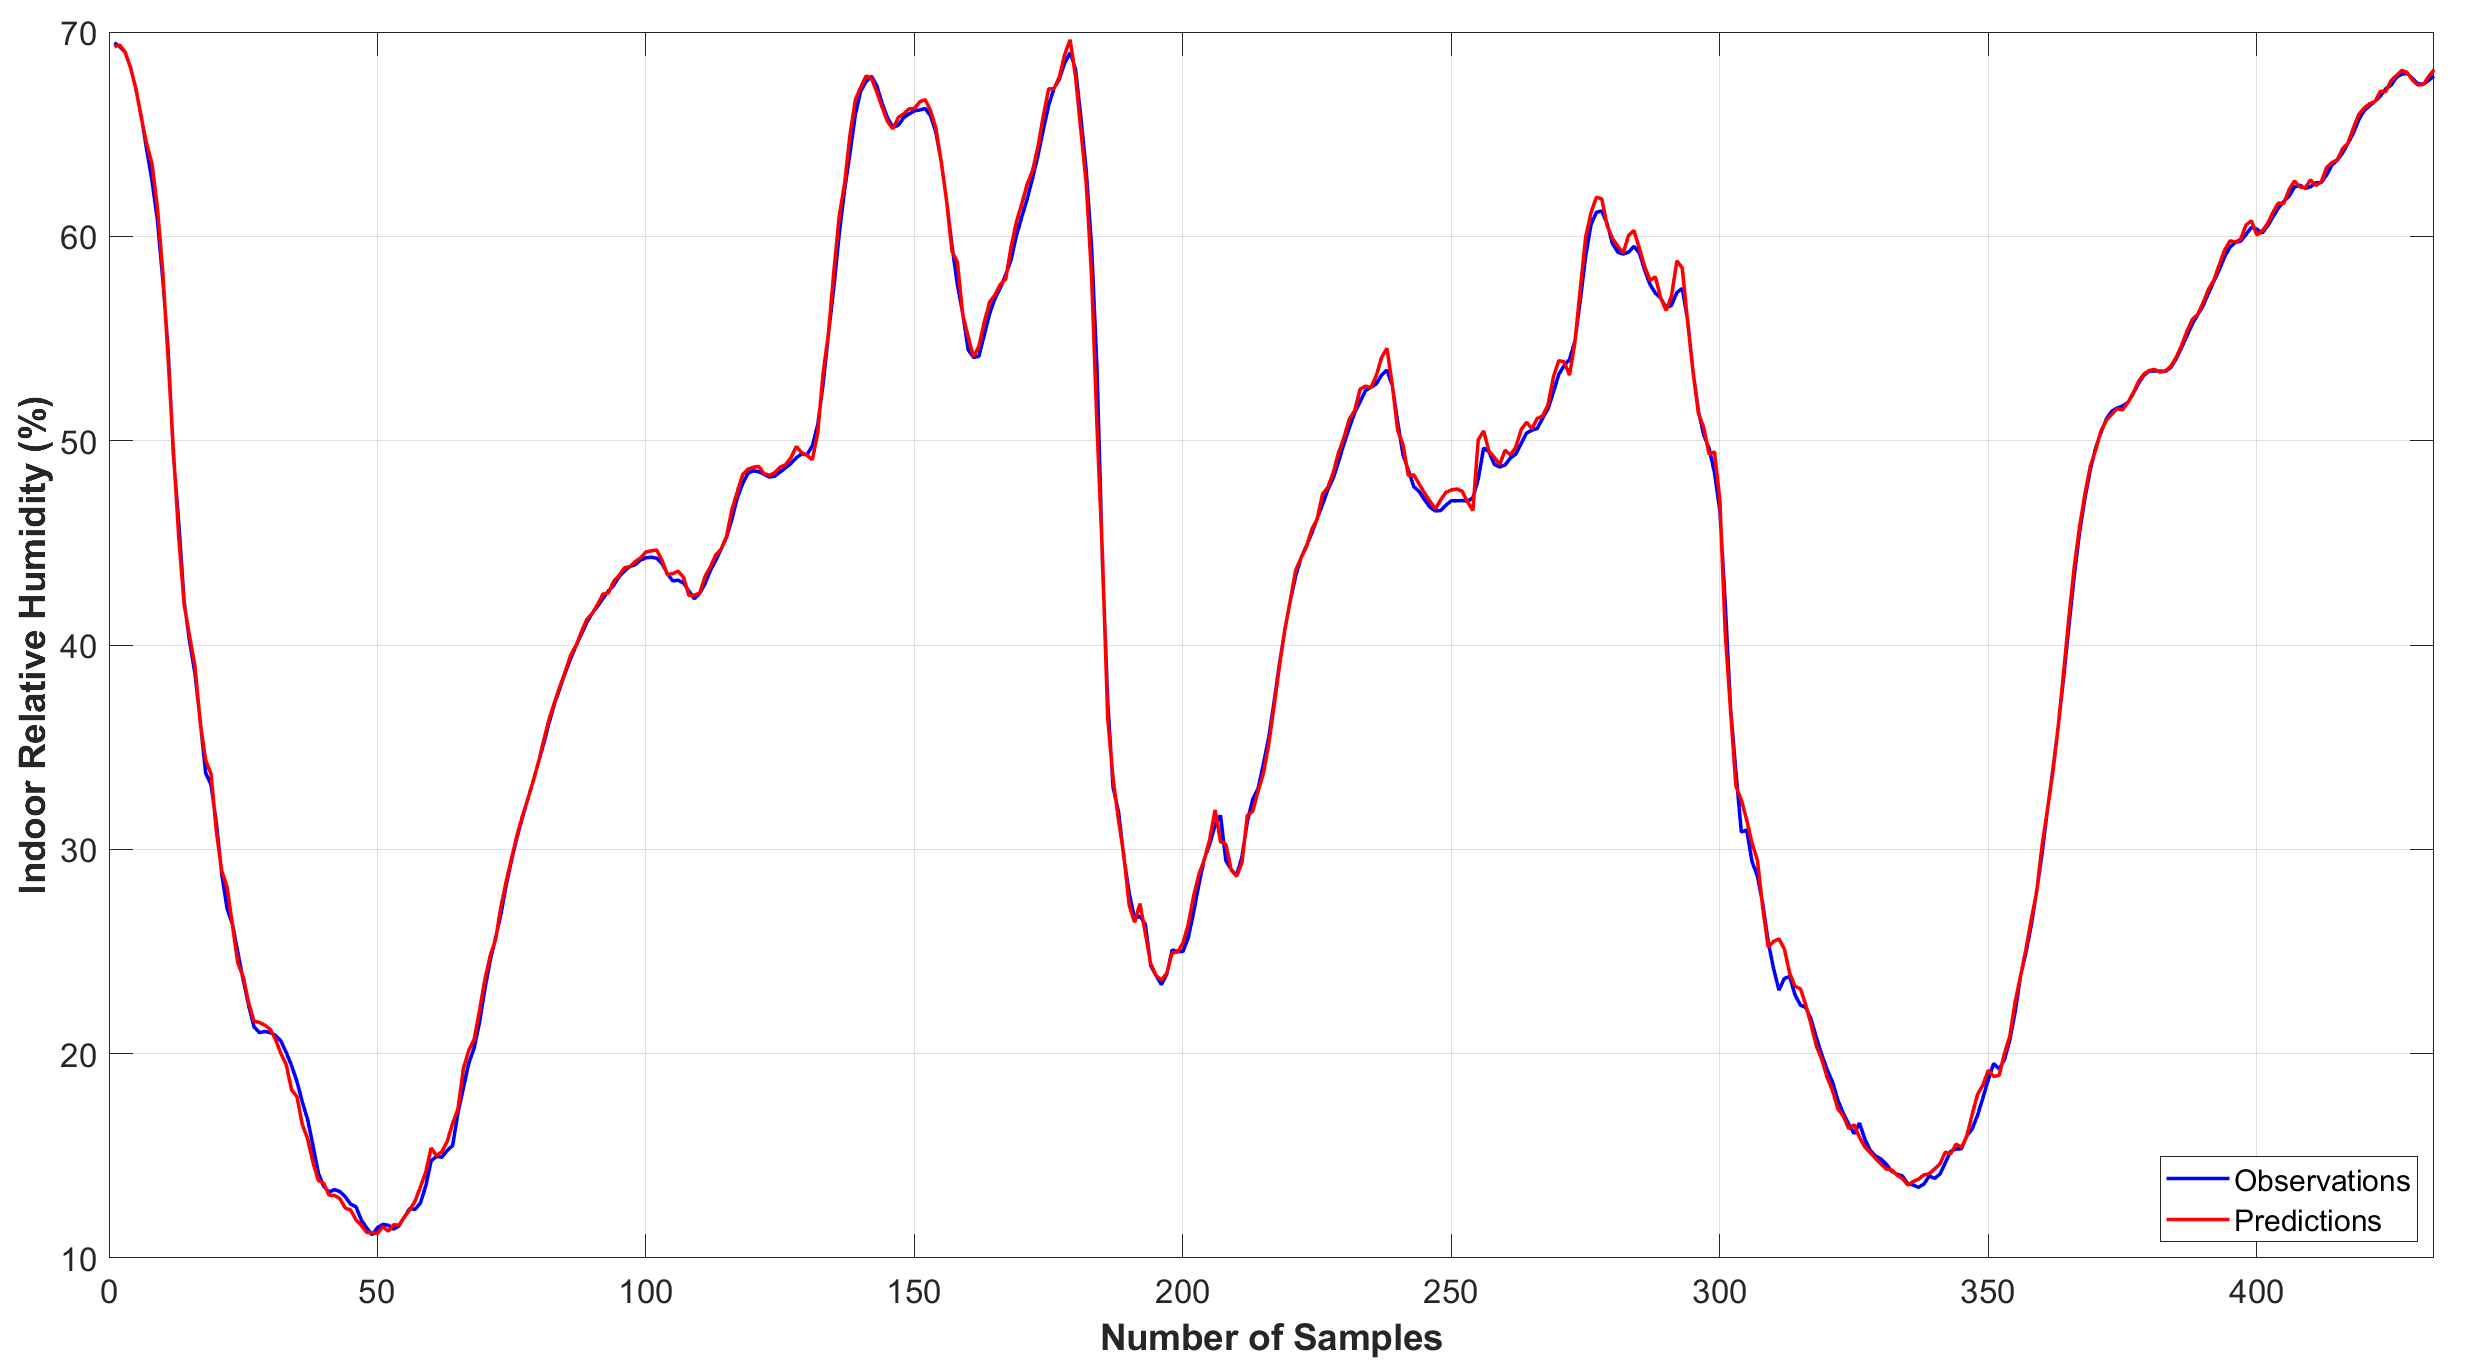
\includegraphics[width=0.9\textwidth]{Figures/NN_RH_in_pred.png}
    \caption{Σύγκριση μεταξύ προβλεπόμενων τιμών και παρατηρήσεων για την σχετική υγρασία εντός του θερμοκηπίου για 
    την περίοδο δοκιμής και δομής νευρωνικού δικτύου 10-7-2.}
    \label{fig_NN_RH_in_pred}
\end{figure}


\begin{figure}[ht]%
    \centering
    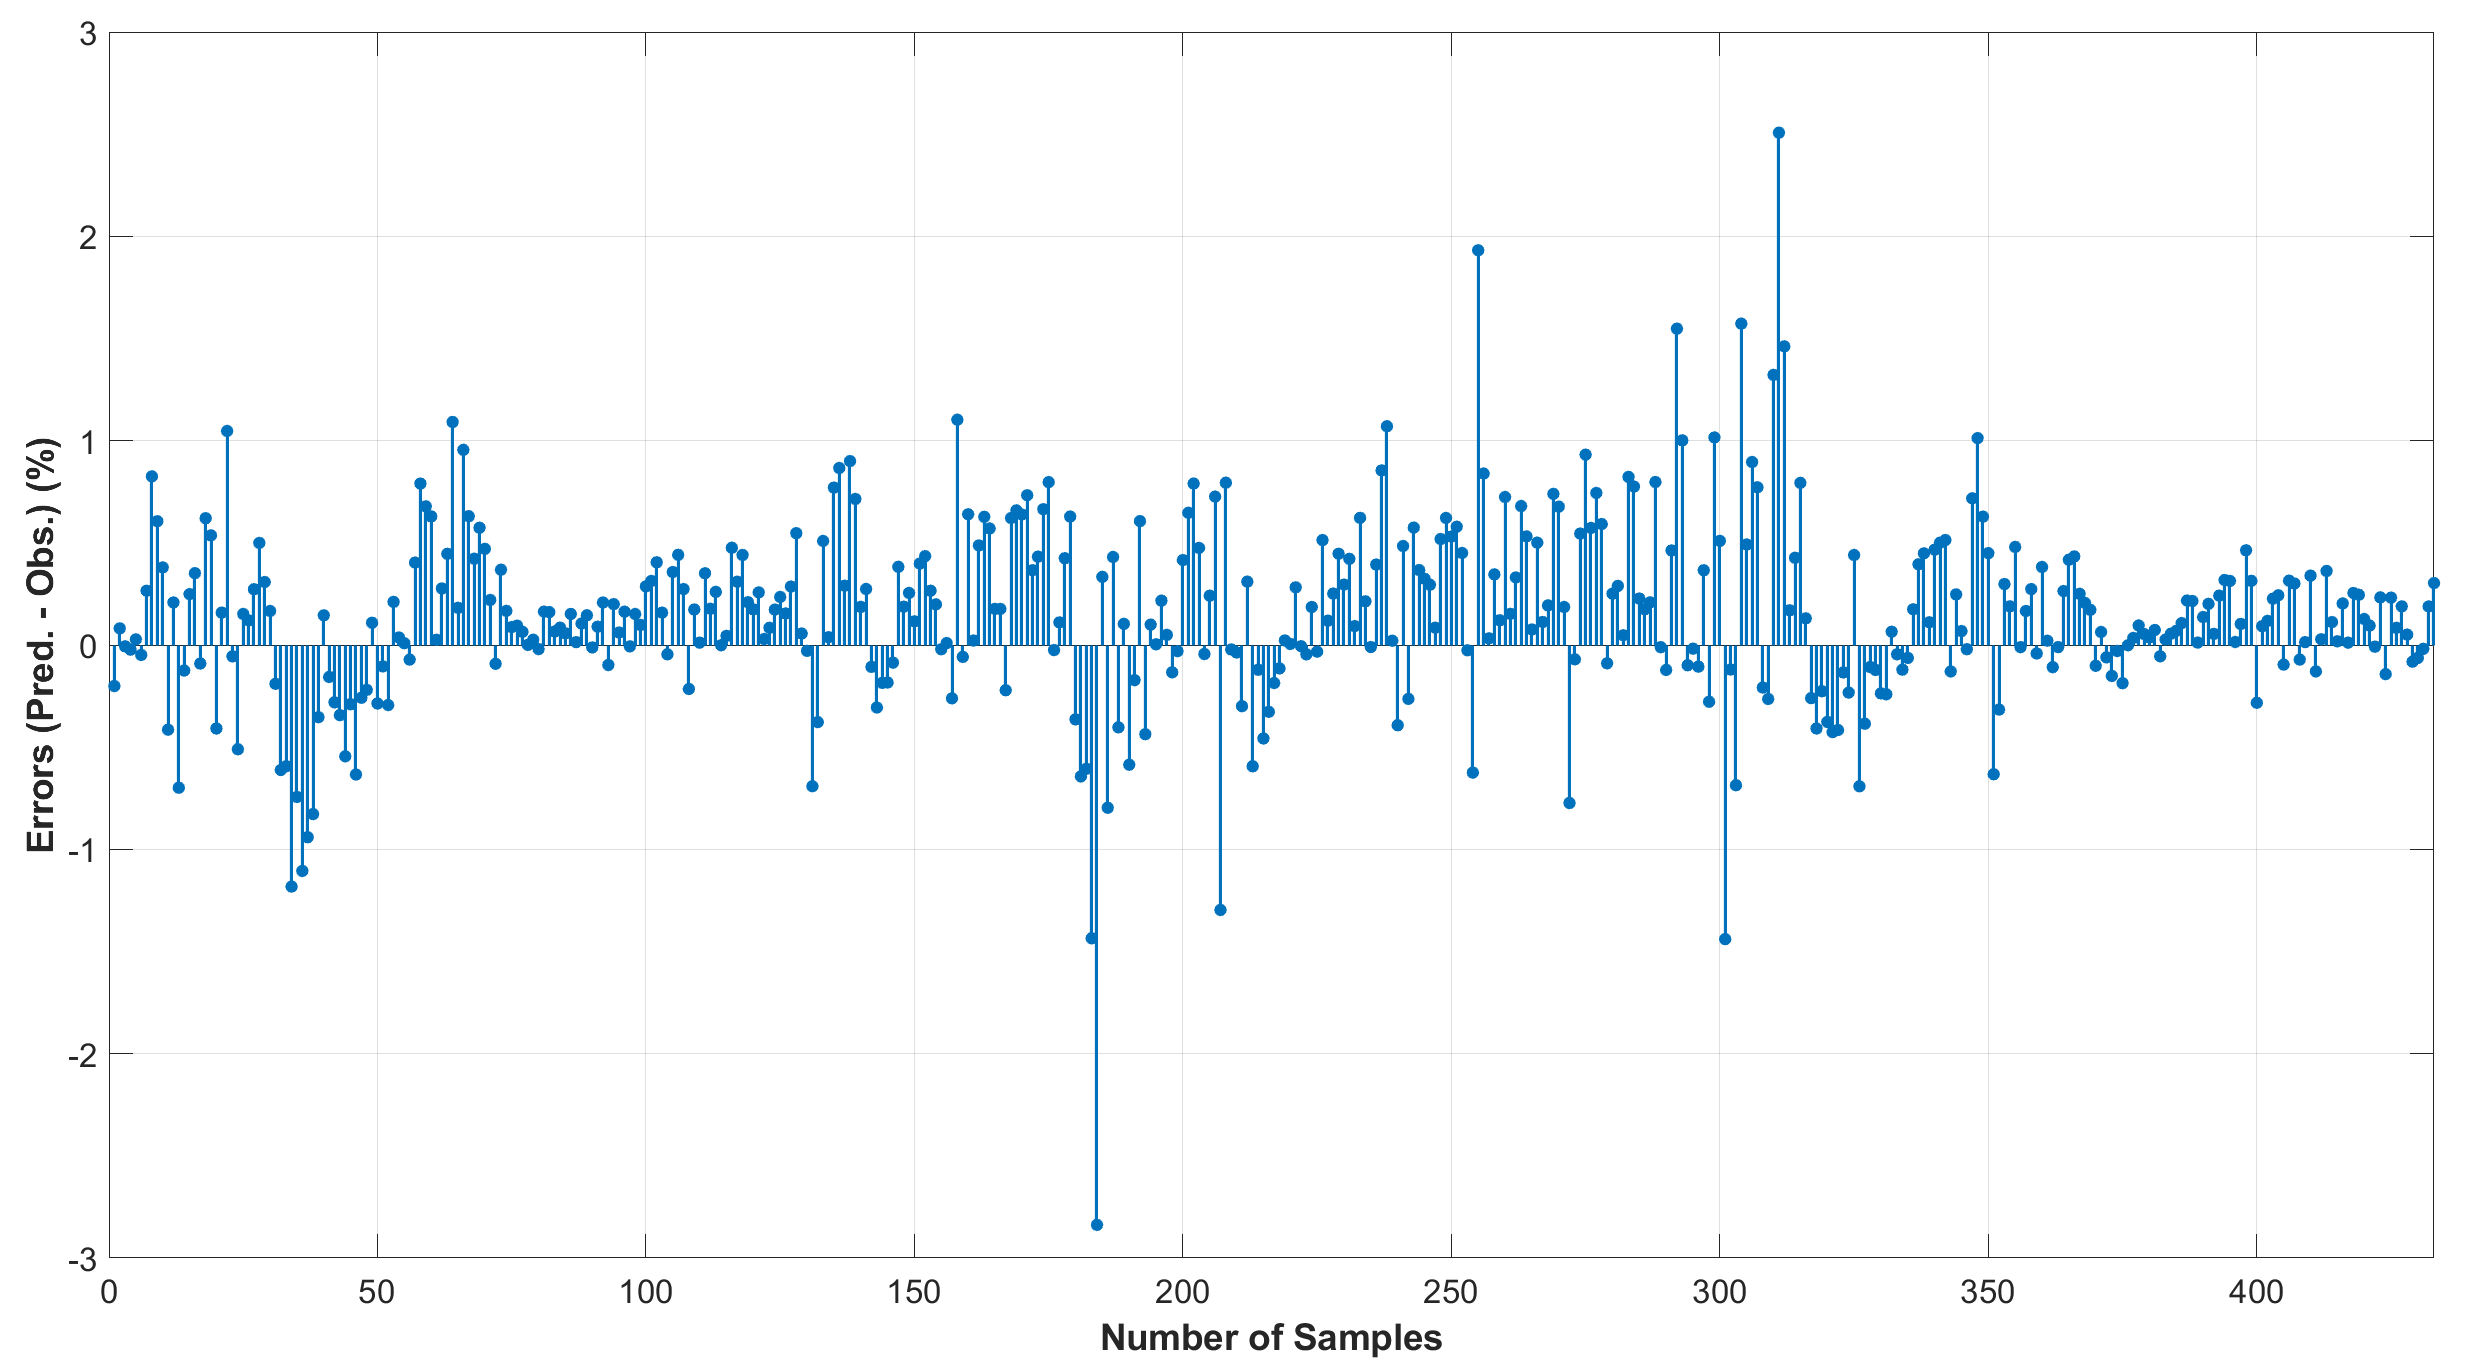
\includegraphics[width=0.9\textwidth]{Figures/NN_RH_in_errors.png}
    \caption{Σφάλματα μεταξύ προβλεπόμενων τιμών και παρατηρήσεων για την σχετική υγρασία εντός του θερμοκηπίου για 
    την περίοδο δοκιμής και δομής νευρωνικού δικτύου 10-7-2.}
    \label{fig_NN_RH_in_errors}
\end{figure}

\clearpage

Στην συγκεκριμένη μελέτη, για την εξαγωγή των βέλτιστων τιμών των παραμέτρων του μοντέλου, χρησιμοποιήθηκαν αρχικά τρεις 
διαφορετικοί αλγόριθμοι εκπαίδευσης, ο αλγόριθμος οπίσθιας τροφοδότησης \english{Levenberg–Marquardt}, ο αλγόριθμος 
οπίσθιας τροφοδότησης Μπαεσιανής κανονικοποίησης και ο αλγόριθμος οπίσθιας τροφοδότησης \english{BFGS Quasi-Newton}, 
με τα αποτελέσματα να δείχνουν ότι ο πρώτος δίνει τις καλύτερες προβλέψεις. Παράλληλα, θα μπορού\-σαν να χρησιμοποιηθούν 
αρκετές ακόμη διαφορετικές τεχνικές βελτιστοποίησης, όπως διαφορετικοί αλγόριθμοι εκπαίδευσης, όπως ο 
“\english{scaled conjugate gradient backpropagation}”, “\english{conjugate gradient with Powell/Beale restarts}”, κ.ά. 
Οι \english{Taki et al.} (\citeyear{neural_bib16}), σε σχετική έρευνα έχουν διενεργήσει σύγκριση ενός μεγάλου πλήθους αλγορίθμων 
εκπαίδευσης, με τον \english{Levenberg–Marquardt backpropagation} να εξάγει τα καλύτερα αποτελέσματα.

Παράλληλα, για την αξιολόγηση των αποτελεσμάτων και τη σύγκριση των προβλεπόμενων και παρατηρούμενων τιμών που αφορούν 
τις δύο παραμέτρους που μελετήθηκαν (εσωτερική θερμοκρασία και σχετική υγρασία) χρησιμοποιήθηκαν τρία διαφορετικά είδη 
περιγραφής των σφαλμάτων. Με αυτόν τον τρόπο επιτεύχθηκε η σύγκριση των αποτελεσμάτων με βάση ένα ευρύ φάσμα μελετών στη 
βιβλιογραφία, καθώς σε κάθε μελέτη χρησιμοποιήθηκε διαφορετικός τύπος για την αξιολόγηση του σφάλματος. Οι υπολογισμένες 
τιμές για το \english{MAE} και το \english{RMSE} βρέθηκαν να είναι αρκετά μικρές, προσδίδοντας ιδιαίτερο βάρος στο 
δημιουργηθέν μοντέλο. Ταυτόχρονα, και μετά από εκτενή έρευνα της βιβλιογραφίας, οι συντελεστές προσδιορισμού, 
\english{R$^2$}, τόσο για τη θερμοκρασία όσο και για τη σχετική υγρασία, αποδείχθηκαν πολύ καλοί, παρουσιάζοντας τιμές 
πολύ κοντά στο 1. Τέλος, το μέγιστο σφάλμα δεν είναι ένας ευρέως διαδεδομένος δείκτης σύγκρισης δεδομένων. Ωστόσο, για 
τις ανάγκες αυτής της εργασίας, ήταν μία πολύ χρήσιμη παράμετρος, με την τιμή του να είναι αρκετά μικρή 
\lcitep{neural_bib21}.

\subsection{Συμπεράσματα}\label{sub_NN_conlusions}

Η μοντελοποίηση του μικροκλίματος του θερμοκηπίου αποδείχθηκε ένα πολύ δύσκολο εγχείρημα λόγω του ότι ένα θερμοκήπιο 
αποτελεί ένα δυναμικό σύστημα άμεσα εξαρτώμενο από τις εξωτερικές περιβαλλοντικές συνθήκες, ενώ οι αλληλεπιδράσεις 
μεταξύ των παραμέτρων που αποτελούν τις εσωτερικές του συνθήκες φαίνεται να είναι τόσο ισχυρές όσο και πολύπλοκες. 
Παρά το γεγονός της ανάπτυξης φυσικών μοντέλων για την εκτίμηση παραμέτρων, όπως η εσωτερική θερμοκρασία και η σχετική 
υγρασία, η πολυπλοκότητά τους δεν τα καθιστά ένα χρήσιμο εργαλείο, ειδικά για τα \english{DSS}, τα οποία απαιτούν 
την χρήση μοντέλων που εκτός από υψηλή ακρίβεια, μπορούν να διαχειριστούν μεγάλα πλήθη δεδομένων με τη μικρότερη δυνατή 
υπολογιστική ισχύ. Οι παραπάνω απαιτήσεις καλύπτονται κατά κύριο λόγο από τη μοντελοποίηση των συνθηκών του θερμοκηπίου 
χρησιμοποιώντας Τεχνητά Νευρωνικά Δίκτυα, για τα οποία η γνώση των φυσικών διεργασιών δεν είναι 
απαραίτητη, προσφέροντας ένα γρήγορο και εύκολο τρόπο αξιολόγησης των επιθυμητών παραμέτρων μέσω των διαδικασιών 
αναγνώρισης συστήματος.

Σκοπός αυτής της μελέτης ήταν η δημιουργία ενός νευρωνικού δικτύου \english{MLP} για την 
εκτίμηση της εσωτερικής θερμοκρασίας και της σχετικής υγρασίας, έχοντας ως μεταβλητές εισόδου την θερμοκρασία και την 
σχετική υγρασία του εξωτερικού περιβάλλοντος, την ταχύτητα του ανέμου, την ηλιακή ακτινοβολία, και την εσωτερική 
θερμοκρασία και σχετική υγρασία με χρονική καθυστέρηση τριών βημάτων. Οι προβλέψεις του μοντέλου μπορούν να 
χρησιμοποιηθούν ως βάση για ένα \english{DSS}. Ο κύριος στόχος ήταν τα μέγιστα σφάλματα των προβλέψεων να είναι όσο το 
δυνατόν μικρότερα, με την τιμή αυτή να παίζει καθοριστικό ρόλο σε ένα \english{DSS}, καθώς ακόμη και μία εσφαλμένη πρόβλεψη 
του μοντέλου είναι πιθανό να καθυστερήσει τη λειτουργία ενός ενεργοποιητή (π.χ. σύστημα θέρμανσης ή δροσισμού) ή ακόμα και 
να μην τον θέσει καθόλου σε λειτουργία, με την καταστροφή της καλλιέργειας να είναι πολύ πιθανή λόγω ακραίων 
συνθηκών. Ταυτόχρονα, μια ακριβής αξιολόγηση των εσωτερικών περιβαλλοντικών παραμέτρων θα επιτρέψει την ενεργοποίηση 
των συστημάτων μόνο όταν αυτό είναι πραγματικά απαραίτητο, με την κατανάλωση της ενέργειας να διατηρείται σε χαμηλά 
επίπεδα.

Πριν από την υλοποίηση του μοντέλου, τα δεδομένα υποβλήθηκαν σε προεπεξεργασία, αφαιρώντας τις ελλείπουσες τιμές και 
κανονικοποιώντας τα σε ένα εύρος από 0,001 έως 0,999 για την αποφυγή σταθμισμένης συνεισφοράς λόγω των διαφορετικών 
μεγεθών των μεταβλητών εισόδου. Για την εκπαίδευση και επικύρωση του μοντέλου, χρησιμοποιήθηκαν 59 ημέρες εκ του συνόλου 
των δεδομένων, τα οποία χωρίστηκαν τυχαία σε δύο υποσύνολα, με το \SI{80}{\percent} να αναφέρεται στη διαδικασία 
εκπαίδευσης και το \SI{20}{\percent} στη διαδικασία επικύρωσης. Οι τρεις εναπομείνουσες ημέρες χρησιμοποιήθηκαν για την 
δοκιμή του μοντέλου. Η δομή του μοντέλου αποτελείται από τρία διαφορετικά επίπεδα, το επίπεδο εισόδου, το κρυφό επίπεδο 
και το επίπεδο εξόδου. Βάσει της μεθόδου δοκιμής και σφάλματος επιλέχθηκε ο αλγόριθμος οπίσθιας τροφοδότησης 
\english{Levenberg–Marquardt}, όντας αυτός που έδωσε τα καλύτερα αποτελέσματα μεταξύ αυτού, του αλγορίθμου οπίσθιας 
τροφοδότησης Μπαεσιανής κανονικοποίησης και του αλγορίθμου οπίσθιας τροφοδότησης \english{BFGS Quasi-Newton}. Ως 
συναρτήσεις ενεργοποίησης χρησιμοποιήθηκαν η λογιστική σιγμοειδής και η γραμμική για το κρυφό επίπεδο και το επίπεδο 
εξόδου, αντίστοιχα. Η λογιστική σιγμοειδής επιλέχθηκε μεταξύ αυτής, της υπερβολικής εφαπτομένης σιγμοειδούς, της 
συνάρτησης ενεργοποίησης ακτινικής βάσης και της θετικής γραμμικής. Το μοντέλο δοκιμάστηκε για διαφορετικό αριθμό κόμβων 
στο κρυφό επίπεδο (από 1 έως 20), με τα καλύτερα αποτελέσματα για την περίοδο δοκιμής να επιτυγχάνονται για τη δομή 
10-7-2. Το μέγιστο σφάλμα ήταν ίσο με \SI{0,877}{\kelvin} και \SI{2,838}{\percent} για τη θερμοκρασία και τη σχετική 
υγρασία αντίστοιχα, ενώ υπολογίστηκαν οι τιμές των \english{MAE}, \english{RMSE} και \english{R$^2$}, με αυτές να 
υπολογίζονται ίσες με \SI{0,218}{\kelvin}, \SI{0,271}{\kelvin} και 0,999 αντίστοιχα, για την θερμοκρασία και ίσες με 
\SI{0,339}{\percent}, \SI{0,481}{\percent} και 0,999 αντίστοιχα για την σχετική υγρασία. Οι παραπάνω τιμές, τόσο για 
το μέγιστο σφάλμα όσο και για τους υπόλοιπους στατιστικούς δείκτες, αποδεικνύουν ότι το συγκεκριμένο μοντέλο μπορεί να 
ικανοποιήσει τις απαιτήσεις ενός συστήματος υποστήριξης λήψης αποφάσεων.

Το προτεινόμενο παραπάνω μοντέλο μπορεί να ανταποκριθεί σε ένα \english{DSS}, καθιστώντας το ένα πολύ σημαντικό 
εργαλείο. Ωστόσο, η ύπαρξη καλλιέργειας μέσα στο θερμοκήπιο θα μπορού\-σε να προκαλέσει προβλήματα στην εξαγωγή 
αξιόπιστων αποτελεσμάτων από το μοντέλο. Η εξέλιξη βιολογικών διεργασιών, όπως η εξατμισοδιαπνοή, θα πρόσθετε έναν 
ακόμα παράγοντα που θα επηρέαζε την θερμοκρασία και την σχετική υγρασία, εκτός από τις συνθήκες του εξωτερικού 
περιβάλλοντος. Ταυτόχρονα, όπως προκύπτει από τα αποτελέσματα, τα μεγαλύτερα σφάλματα του μοντέλου παρουσιάζονται τη 
στιγμή που τόσο η θερμοκρασία όσο και η σχετική υγρασία εμφανίζουν απότομες αλλαγές. Ως εκ τούτου, η ικανότητα του 
μοντέλου να προβλέπει τις παραπάνω παραμέτρους θα πρέπει να μελετηθεί και στην περίπτωση που η παρουσία ενεργοποιητών 
(π.χ. συστήματα θέρμανσης, δυναμικός εξαερισμός) δύναται να προκαλεί σχετικά απότομες αλλαγές στο μικροκλίμα του 
θερμοκηπίου. Τέλος, η προσθήκη δεδομένων που περιγράφουν ακραίες συνθήκες, όπως οι θερμοκρασίες κατά την διάρκεια ενός 
καλοκαιρινού καύσωνα, ή κατά την διάρκεια μίας εξαιρετικά κρύας ημέρας του χειμώνα, θα μπορούσε να εκπαιδεύσει το 
μοντέλο σε ακραίες περιπτώσεις που θα υπήρχε περίπτωση να προκαλέσουν σημαντικά προβλήματα στην καλλιέργεια. Μελλοντικές 
εργασίες θα μπορούσαν να περιλάβουν τη μελέτη της ικανότητας του μοντέλου να προβλέπει τη θερμοκρασία και τη σχετική 
υγρασία υπό την επίδραση μιας καλλιέργειας θερμοκηπίου, την προσθήκη παραμέτρων που αφορούν τους ενεργοποιητές του 
θερμοκηπίου, αλλά και την προσθήκη περισσότερων δεδομένων στο μοντέλο για την εκπαίδευσή του σε περαιτέρω περιπτώσεις, 
καθώς και την απόκτηση ικανότητας να ανταποκρίνεται σε ακραίες συνθήκες και γρήγορες δυναμικές αλλαγές.

%%%%%%%%%%%%%%%%%%%%%%%%%%%%%%%%%%%%%%%%%%
%%%%%%%%%%%%%%%%%%%%%%%%%%%%%%%%%%%%%%%%%%
\newpage
\vspace*{6.5cm}
\sloppy
\section{Αλγόριθμος για τον υπολογισμό της σκίασης που δημιουργείται από φωτοβολταϊκά ενσωματωμένα στο 
θερμοκήπιο}\label{sec_algorithm}
\fussy

Οι αλγόριθμοι μοντελοποίησης της σκίασης είναι κρίσιμης σημασίας για την πρόβλεψη της απόδοσης των ημιδιαφανών 
φωτοβολταϊκών σε θερμοκήπια. Οι ακριβείς προβλέψεις των μοτίβων σκίασης μπορούν να βοηθήσουν στη βελτιστοποίηση 
της θέσης και του προσανατολισμού των φωτοβολταϊκών, επιτρέποντας τη μέγιστη έκθεση των φυτών στο φως. Επιπλέον, 
αυτοί οι αλγόριθμοι μπορούν να παρέχουν πληροφορίες σχετικά με τις επιπτώσεις της σκίασης σε διαφορετικά είδη 
καλλιεργειών και στάδια ανάπτυξης, βοηθώντας στη λήψη αποφάσεων για τη διαχείριση του θερμοκηπίου.

Υπάρχουν διάφοροι τύποι αλγορίθμων μοντελοποίησης της σκίασης, συμπεριλαμβανομένων αναλυτικών, αριθμητικών και 
υβριδικών προσεγγίσεων. Οι αναλυτικές μέθοδοι χρησιμοποιούν μαθηματικές εξισώσεις, βασισμένες στην τριγωνομετρία, 
τη διανυσματική ανάλυση \lcitep{algorithm_bib1} και τη γραμμική άλγεβρα για τον υπολογισμό της ποσότητας σκιάς που 
σχηματίζεται σε μια φωτοβολταϊκή συστοιχία ή θερμοκήπιο \lcitep{algorithm_bib2}, ενώ οι αριθμητικές μέθοδοι 
\lcitep{algorithm_bib3} χρησιμοποιούν προσομοιώσεις και υπολογιστικά μοντέλα για την πρόβλεψη μοτίβων και έντασης της 
σκιάς. Οι υβριδικές μέθοδοι συνδυάζουν αναλυτικές και αριθμητικές μεθόδους για να παρέχουν ακριβή και αποτελεσματική 
μοντελοποίηση της σκίασης.

Οι βασικές κατηγορίες αλγορίθμων που χρησιμοποιούνται για τη μοντελοποίηση φαινομένων σκίασης από ημιδιαφανή 
φωτοβολταϊκά σε θερμοκήπια είναι:

\begin{enumerate}
    \item \textbf{Αλγόριθμοι ανίχνευσης ακτινών (\english{Ray-tracing algorithms}):} Αυτοί οι αλγόριθμοι βασίζονται 
    στην προσομοίωση της συμπεριφοράς των ακτινών φωτός και των αλληλεπιδράσεών τους με τις επιφάνειες των θερμοκηπιακών 
    και φωτοβολταϊκών μονάδων. Μπορούν να παρέχουν ακριβείς προβλέψεις των αποτελεσμάτων σκίασης υπό διαφορετικές 
    συνθήκες \lcitep{algorithm_bib4,algorithm_bib5}.
    \item \textbf{Αλγόριθμοι βάσει της μεθόδου πεπερασμένων στοιχείων (\english{Finite Element Method – FEM – 
    algorithms}):} Η μέθοδος των Πεπερασμένων Στοιχείων είναι μια αριθμητική μέθοδος που χρησιμοποιείται για την 
    επίλυση διαφορικών εξισώσεων. Στην περίπτωση των φωτοβολταϊκών θερμοκηπίων, οι συγκεκριμένοι αλγόριθμοι μπορούν 
    να χρησιμοποιηθούν για τη μοντελοποίηση της αλληλεπίδρασης μεταξύ του φωτός και της δομής του θερμοκηπίου, 
    συμπεριλαμβανομένων των ημιδιαφανών φωτοβολταϊκών πλαισίων \lcitep{algorithm_bib6,algorithm_bib7,algorithm_bib8}.
    \item \textbf{Αλγόριθμοι μοντελοποίησης σκιάς (\english{Shadow modeling algorithms}):} Αυτοί οι αλγόριθμοι 
    βασίζονται στον υπολογισμό της θέσης του ήλιου στον ουρανό για οποιαδήποτε δεδομένη στιγμή, προκειμένου να 
    ληφθεί η προβολή της σκιάς για οποιοδήποτε σημειακό ή μη αντικείμενο. Χρησιμοποιούν μια διαδικασία ραστεροποίησης 
    για να αξιολογήσουν τη σκιασμένη περιοχή μιας διάταξης και μπορούν να παρέχουν μοτίβα σκίασης για ένα επιθυμητό 
    χρονικό διάστημα \lcitep{algorithm_bib9,algorithm_bib10}.
    \item \textbf{Αλγόριθμοι κατανομής φωτός (\english{Light distribution algorithms}):} Αυτοί οι αλγόριθμοι 
    χρησιμοποιούνται για την εκτίμηση της ολικής ηλιακής ακτινοβολίας μέσα στα φωτοβολταϊκά θερμοκήπια και για 
    επιθυμητό χρονικό διάστημα. Υπολογίζουν την άμεση και σκεδαζόμενη ακτινοβολία σε διάφορα σημεία παρατήρησης 
    μέσα στο φωτοβολταϊκό θερμοκήπιο και μπορούν να παρέχουν χάρτες της κατανομής του φωτός σε διαφορετικά ύψη 
    \lcitep{algorithm_bib11,algorithm_bib12}.
\end{enumerate}

\noindent Αυτοί οι αλγόριθμοι έχουν διαφορετικά πλεονεκτήματα και αδυναμίες και μπορούν να εφαρμοστούν σε διάφορους 
τύπους φωτοβολταϊκών θερμοκηπίων ανάλογα με τις ειδικές απαιτήσεις του εκάστοτε έργου.

Αρκετές μελέτες έχουν προτείνει αλγόριθμους για την εκτίμηση της επίδρασης σκίασης των φωτοβολταϊκών πάνελ στις 
καλλιέργειες μέσα σε θερμοκήπια. Οι \english{de Sá et al.} (\citeyear{algorithm_bib9}) πρότειναν έναν αλγόριθμο 
μοντελοποίησης σκιάς βασισμένο στον υπολογισμό της θέσης του ήλιου στον ουρανό και σε μια διαδικασία ραστεροποίησης 
για την αξιολόγηση της σκιασμένης περιοχής της φωτοβολταϊκής συστοιχίας. Ο αλγόριθμος μπορεί να παρέχει μοτίβα 
σκίασης για ένα επιθυμητό εύρος χρόνου και να υπολογίζει τον ρυθμό απόδοσης της ισχύος της προσπίπτουσας ακτινοβολίας 
στη συστοιχία σε σύγκριση με τη περίπτωση μη σκίασης. Ο αλγόριθμος έχει ενδιαφέρουσες εφαρμογές, όπως η βελτιστοποίηση 
της θέσης και του προσανατολισμού της συστοιχίας, η αξιολόγηση της επίδρασης νέων εμποδίων σε προϋπάρχουσες 
εγκαταστάσεις, επιτρέποντας την απόκτηση ακριβών και πρακτικών δεδομένων με σκοπό την δημιουργία στρατηγικών ελέγχου 
και τεχνικών \english{MPPT (Maximum Power Point Tracking)} για μερικώς σκιασμένα συστήματα, υπολογίζοντας πιο ρεαλιστικά 
περιορισμένα σενάρια απόσβεσης και βρίσκοντας τη βέλτιστη διασύνδεση της φωτοβολταϊκής συστοιχίας. 

Οι \english{Cossu et al.} (\citeyear{algorithm_bib11}) έχουν αναπτύξει έναν αλγόριθμο για την εκτίμηση της ολικής 
ηλιακής ακτινοβολίας μέσα σε φωτοβολταϊκά θερμοκήπια για ένα επιθυμητό χρονικό διάστημα. Ο αλγόριθμος λαμβάνει υπόψη 
την άμεση και σκεδαζόμενη ακτινοβολία σε διάφορα σημεία παρατήρησης μέσα στο φωτοβολταϊκό θερμοκήπιο, με τις 
φωτοβολταϊκές μονάδες να εξομοιώνονται με πολύγωνα που μπορούν να επικαλύψουν την πορεία του ήλιου ως προς ένα 
συγκεκριμένο σημείο παρατήρησης. Ο αλγόριθμος δοκιμάστηκε σε θερμοκήπιο με αναλογία φωτοβολταϊκής κάλυψης 
\SI{50}{\percent} στην οροφή και τα αποτελέσματα χρησιμοποιήθηκαν για τη σχεδίαση χαρτών της κατανομής του φωτός σε 
διαφορετικά ύψη του θόλου. Ο αλγόριθμος μπορεί να χρησιμοποιηθεί ως ένα εργαλείο υποστήριξης λήψης αποφάσεων για τον 
προσδιορισμό των καταλληλότερων ειδών καλλιέργειας με βάση τις απαιτήσεις τους σε φωτισμό.

Σε αυτή τη μελέτη παρουσιάζεται ένας αλγόριθμος που αναπτύχθηκε για τον υπολογισμό της σκιασμένης επιφάνειας που 
προκαλείται από φωτοβολταϊκές μονάδες εντός του θερμοκηπίου. Ο αλγόριθμος βασίστηκε σε μια ήδη υπάρχουσα εγκατάσταση 
φωτοβολταϊκού συστήματος σε θερμοκήπιο, με τη δυνατότητα επέκτασής του σε διαφορετικές μονάδες. Οι γραφικές 
αναπαραστάσεις που εξάγει παράλληλα ο αλγόριθμος μπορούν να χρησιμοποιηθούν για να διευκολύνουν την κατανόηση των 
αποτελεσμάτων. 

Παρά το γεγονός ότι έχουν ήδη αναπτυχθεί μοντέλα για τον εντοπισμό της σκίασης από διάφορα αντικείμενα, καθώς και 
τη μελέτη της κατανομής ακτινοβολίας μέσα σε ένα θερμοκήπιο και υπό την επίδραση φωτοβολταϊκών μονάδων, υπάρχει ένα 
κενό στη βιβλιογραφία σχετικά με τη λεπτομερή μοντελοποίηση της σκιασμένης περιοχής μέσα σε ένα θερμοκήπιο λόγω 
φωτοβολταϊκών. Ο υπολογισμός και η οπτικοποίηση της σκιασμένης επιφάνειας για θερμοκήπια τύπου \english{even-span} και 
Αγριβολταϊκών οποιουδήποτε μεγέθους είναι ένα σημαντικό εργαλείο για τους παραγωγούς και τους χρήστες τέτοιων συστημάτων, 
ενώ ο συνδυασμός αυτού του αλγορίθμου με υπάρχοντα μοντέλα θα μπορούσε να οδηγήσει στην πλήρη καταγραφή της σκίασης από 
φωτοβολταϊκά πλαίσια σε θερμοκήπια. Ταυτόχρονα, η χρήση του αλγορίθμου πριν από την εγκατάσταση φωτοβολταϊκών, ή ακόμα 
και πριν από την κατασκευή της πλήρους θερμοκηπιακής μονάδας, θα παρείχε ένα πρόσθετο όφελος στους χρήστες, δημιουργώντας 
τις ιδανικές συνθήκες για την επιθυμητή καλλιέργεια. Τέλος, η προσπάθεια παροχής απλών και ξεκάθαρων αποτελεσμάτων 
επιτρέπει τη χρήση της μεθόδου από τον οποιονδήποτε, χωρίς την απαίτηση επιπλέον γνώσεων σχετικά με τα επιστημονικά 
πλαίσια που σχετίζονται με την ακτινοβολία και τη διάδοσή της, ή τη γεωμετρία των σχετικών συστημάτων.

\subsection{Μεθοδολογία}\label{sub_alg_methods}

Στη μελέτη αυτή παρουσιάζεται ένας αλγόριθμος, βάσει του οποίου είναι δυνατή η εκτίμηση της συνολικής σκίασης 
που προκαλείται από φωτοβολταϊκά πλαίσια ενσωματωμένα στην οροφή ενός αμφίρρικτου θερμοκηπίου. Ο αλγόριθμος είναι 
ουσιαστικά μια μητρική συνάρτηση (\english{parent function}), αποτελούμενη από πέντε ένθετες συναρτήσεις 
(\english{nested functions}), καθώς και τέσσερα τμήματα μεμονωμένων εντολών για τον αριθμό και τη θέση των 
φωτοβολταϊκών στην οροφή. Τα τελικά εξαχθέντα αποτελέσματα του αλγορίθμου αφορούν τον υπολογισμό της σκιασμένης 
επιφάνειας από τα φωτοβολταϊκά εντός της επιθυμητής κατασκευαστικής θερμοκηπιακής μονάδας, το ποσοστό της 
σκιασμένης επιφάνειας επί της συνολικής επιφάνειας της κατασκευαστικής μονάδας, καθώς και δύο γραφήματα. Το πρώτο γραφημα 
με την τρισδιάστατη (\english{3D}) οπτικοποίηση του θερμοκηπίου, των φωτοβολταϊκών και της σχηματισμένης σκιάς σε 
ένα Καρτεσιανό σύστημα συντεταγμένων, και το δεύτερο με την κάτοψη όλων των παραπάνω σε ένα δισδιάστατο 
(\english{2D}) Kαρτεσιανό σύστημα συντεταγμένων. Η εκτίμηση της σκιάς μπορεί να γίνει μέχρι και ένα χρονικό βήμα, 
\english{$t$}, ίσο με 10 λεπτά για κάθε χρονική περίοδο μέσα στο έτος, με τον αλγόριθμο να ενσωματώνει κριτήρια που 
της απαγορεύουν να λειτουργεί για ενδιάμεσα χρονικά διαστήματα ή περιστάσεις όπου δεν υφίστανται ημερολογιακά ή 
γεωγραφικά. Τα ανωτέρω κριτήρια παρουσιάζονται στον Πίνακα \ref{tab_alg_kritiria}. Όλες οι διαδικασίες που 
χρησιμοποιήθηκαν για τις συναρτήσεις περιγράφονται παρακάτω, μαζί με τις συναρτήσεις όπως αυτές υλοποιήθηκαν με 
χρήση της γλώσσας προγραμματισμού \english{MATLAB}.

\begin{table}[ht]
    \centering
    \caption{Ημερολογιακά και γεωγραφικά κριτήρια στον αλγόριθμο.}\label{tab_alg_kritiria} 
    \begin{tabular*}{\textwidth}{{@{\extracolsep\fill}cccl}}
        \toprule
        \textbf{Συνθήκη} & \textbf{Μεταβλητή} & \textbf{Κριτήριο} & \textbf{Κώδικας \english{MATLAB}} \\
        \midrule
        
        \multirow{9}{*}{\makecell{Ημερομηνία/\\Ώρα}} 
        & \multirow{2}{*}{\makecell{Ημέρες}} & \texttt{\english{Day = [1:1:last}} & \texttt{\english{if d<1 || d>eomday(yr,mth)}} \\ & & \texttt{\english{day of month]}} & \texttt{\english{\ \ \ \ error();}} \\
            
        & \multirow{2}{*}{\makecell{Ώρες}} & \multirow{2}{*}{\makecell{\texttt{\english{Hour = [0:1:23]}}}} & \texttt{\english{if hr<0 || hr>23}} \\ 
        & & & \texttt{\english{\ \ \ \ error();}} \\
        
        & \multirow{2}{*}{\makecell{Λεπτά}} & \multirow{2}{*}{\makecell{\texttt{\english{Minute = [0:10:50]}}}} & \texttt{\english{if mnt $\sim$ [0:10:50]}} \\ 
        & & & \texttt{\english{\ \ \ \ error();}} \\
        
        & \multirow{2}{*}{\makecell{Δευτερόλεπτα}} & \multirow{2}{*}{\makecell{\texttt{\english{Second = 0}}}} & \texttt{\english{if sc $\sim$ 0}} \\ 
        & & & \texttt{\english{\ \ \ \ error();}} \\
        
        \hline
        
        \multirow{4}{*}{Τόπος} 
        & \multirow{2}{*}{\makecell{Γεωγρ. Μήκος}} & \multirow{2}{*}{\makecell{\texttt{\english{Longitude = [0,360]}}}} & \texttt{\english{if lon<0 || lon>360}} \\ 
        & & & \texttt{\english{\ \ \ \ error();}} \\
        
        & \multirow{2}{*}{\makecell{Γεωγρ. Πλάτος}} & \multirow{2}{*}{\makecell{\texttt{\english{Latitude = [-90,90]}}}} & \texttt{\english{if lat<-90 || lat>90}} \\ 
        & & & \texttt{\english{\ \ \ \ error();}} \\
        \hline
    \end{tabular*}
\end{table}

Οι ένθετες συναρτήσεις που εφαρμόστηκαν αφορούν τη θέση του Ήλιου, όπως αυτή μπορεί να υπολογιστεί σε ένα σφαιρικό 
σύστημα συντεταγμένων (Συνάρτηση 1 – \english{Function} 1), την απόσταση μεταξύ της Γης και του Ήλιου 
(Συνάρτηση 2 – \english{Function} 2), τα αποτελέσματα της οποίας χρησιμοποιούνται για τη μετατροπή της θέσης του Ήλιου 
από σφαιρικές σε Καρτεσιανές συντεταγμένες (Συνάρτηση 3 – \english{Function} 3). Στη συνέχεια, υπολογίζονται οι 
συντεταγμένες των σημείων που απαρτίζουν το θερμοκήπιο σε ένα Kαρτεσιανό σύστημα συντεταγμένων (Συνάρτηση 4 – 
\english{Function} 4) που βασίζεται σε βασικά χαρακτηριστικά του θερμοκηπίου, όπως ο αριθμός των κατασκευαστικών 
μονάδων, οι οποίες επαναλαμβάνονται είτε κατά πλάτος είτε κατά μήκος, το μήκος της κατασκευαστικής μονάδας, το πλάτος 
της, το ύψος της υδρορροής και του κορφιά. Η τελευταία ένθετη συνάρτηση που δημιουργήθηκε και χρησιμοποιήθηκε είναι 
αυτή που αφορά την εύρεση της σκιάς που σχηματίζεται από τα φωτοβολταϊκά (Συνάρτηση 5 – \english{Function} 5).

Τα επιμέρους τμήματα του αλγορίθμου που υλοποιήθηκαν αφορούν τις συντεταγμένες των σημείων που αντιστοιχούν στις 
τέσσερις γωνίες κάθε φωτοβολταϊκής μονάδας, ανάλογα με τη θέση τους στην οροφή του θερμοκηπίου, τόσο για την πρώτη 
όσο και για τη δεύτερη μονάδα στην οποία έχουν τοποθετηθεί τα φωτοβολταϊκά (Τμήμα του κώδικα 1 – 
\english{Part of the code} 1), τη δυαδική αναπαράσταση της επιφάνειας που καλύπτει το θερμοκήπιο και την επιφάνεια 
του εδάφους του θερμοκηπίου που σκιάζεται από τα φωτοβολταϊκά (Τμήμα του κώδικα 2 – \english{Part of the code} 2), 
και τον υπολογισμό της σκιασμένης περιοχής εντός της καλλιεργήσιμης έκτασης του θερμοκηπίου (Τμήμα του κώδικα 3 – 
\english{Part of the code} 3). Τέλος, έχει εφαρμοστεί ένα μέρος του κώδικα, το οποίο έχει τη δυνατότητα εξαγωγής 
αποτελεσμάτων σχετικά με το αν ένα σημείο βρίσκεται εντός ή εκτός της σκιασμένης επιφάνειας για δεδομένο χρονικό 
διάστημα (Τμήμα του κώδικα 4 – \english{Part of the code} 4). Αυτό το τμήμα του κώδικα λειτουργεί προαιρετικά, 
ανάλογα με το αν εισάγονται ή όχι οι αντίστοιχες τιμές εισόδου στον αλγόριθμο.

Το παρακάτω διάγραμμα ροής παρουσιάζει τη σειρά με την οποία εμφανίζονται οι Συναρτήσεις και τα Τμήματα του κώδικα 
στον αλγόριθμο.

\noindent
\begin{tikzpicture}[node distance=2cm]
    \centering
    \node (input) [io] {\textbf{Δεδομένα εισόδου}};
    \node (fnc1) [process, below of=input] {
      \textbf{Συνάρτηση 1}\\
      \textit{Υπολογισμοί για την θέση του Ήλιου σε σφαιρικές συντεταγμένες}
    };
    \node (fnc2) [process, below of=fnc1] {
      \textbf{Συνάρτηση 2}\\
      \textit{Υπολογισμός της απόστασης Γης-Ήλιου}
    };
    \node (fnc3) [process, below of=fnc2] {
      \textbf{Συνάρτηση 3}\\
      \textit{Μετασχηματισμός από σφαιρικό σε Καρτεσιανό σύστημα συντεταγμένων}
    };
    \node (fnc4) [process, below of=fnc3] {
      \textbf{Συνάρτηση 4}\\
      \textit{Υπολογισμός των συντεταγμένων του θερμοκηπίου}
    };
    \node (prt1) [process, below of=fnc4] {
      \textbf{Τμήμα του κώδικα 1}\\
      \textit{Υπολογισμός των συντεταγμένων των Φ/Β}
    };
    \node (fnc5) [process, below of=prt1] {
      \textbf{Συνάρτηση 5}\\
      \textit{Υπολογισμός των σημείων που σχηματίζουν την σκιά}
    };
    \node (prt2a) [process, below of=fnc5] {
      \textbf{Τμήμα του κώδικα 2A} \\
      \textit{Δυαδική ανάλυση - Αναπαράσταση του θερμοκηπίου}
    };
    \node (prt2b) [process, below of=prt2a] {
      \textbf{Τμήμα του κώδικα 2B} \\
      \textit{Δυαδική ανάλυση - Αναπαράσταση της σκιάς}
    };
    \node (prt3) [process, below of=prt2b] {
      \textbf{Τμήμα του κώδικα 3} \\
      \textit{Υπολογισμός σκιασμένης επιφάνειας του θερμοκηπίου}
    };
    \node (prt4) [process, below of=prt3] {
      \textbf{Τμήμα του κώδικα 4} \\
      \textit{Σκιασμένα ή μη σημεία επιφάνειας του θερμοκηπίου}
    };
    \node (output) [io, right of=prt4, xshift=6.2cm] {
      \textbf{Δεδομένα εξόδου}
    };
    
    \draw [arrow] (input) -- (fnc1);
    \draw [arrow] (fnc1) -- (fnc2);
    \draw [arrow] (fnc2) -- (fnc3);
    \draw [arrow] (fnc3) -- (fnc4);
    \draw [arrow] (fnc4) -- (prt1);
    \draw [arrow] (prt1) -- (fnc5);
    \draw [arrow] (fnc5) -- (prt2a);
    \draw [arrow] (prt2a) -- (prt2b);
    \draw [arrow] (prt2b) -- (prt3);
    \draw [arrow] (prt3) -| (output);
    \draw [arrow] (prt3) -- node[anchor=east] {\textbf{Προαιρετικά}} (prt4);
    \draw [arrow] (prt4) -- (output);
\end{tikzpicture}

\vspace{0.2cm}

Αν και οι Συναρτήσεις 4 και 5 μπορούν να χρησιμοποιηθούν για οποιαδήποτε περίπτωση θερμοκηπίου και χωροθέτησης 
φωτοβολταϊκών στη οροφή του, η χρήση τους στην παρούσα έρευνα αφορά μία συγκεκριμένη περίπτωση θερμοκηπίου και 
θέσεις φωτοβολταϊκών. Το θερμοκήπιο που χρησιμοποιήθηκε στην έρευνα περιγράφεται στην Παράγραφο 
\ref{sub_thermokipio}, ενώ τα φωτοβολταϊκά στην Παράγραφο \ref{sub_PVs}, με τις χαρακτηριστικές τιμές διαφόρων 
στοιχείων τους να δίνονται στους Πίνακες \ref{tab_greenhouse_characteristics} και \ref{tab_PV_characteristics}, 
αντίστοιχα.

\subsubsection{Υπολογισμοί για την θέση του Ήλιου}\label{subsub_Sun_position}

Ξεκινώντας από έναν από τους πιο θεμελιώδεις παράγοντες, η θέση του ήλιου στον ουρανό μπορεί να οριστεί από δύο 
ξεχωριστές γωνίες σε ένα σφαιρικό σύστημα συντεταγμένων, την ηλιακή ζενίθια γωνία (\english{Solar Zenith Angle – SZA}) 
και την ηλιακή αζιμούθια γωνία (\english{Solar Azimuth Angle – SAA}) \lcitep{algorithm_bib13}. Η \english{SZA} ορίζεται 
ως η γωνία που σχηματίζεται από τη γραμμή που διέρχεται μεταξύ του ήλιου και της υπό μελέτη περιοχής στη Γη και την 
κάθετη γραμμή προς την ίδια περιοχή (ο άξονας $\english{z}$ σε ένα Καρτεσιανό σύστημα συντεταγμένων). Μπορεί επίσης 
να οριστεί ως η γωνία με την οποία η ακτινοβολία δέσμης χτυπά τη γη. Μπορεί επίσης να οριστεί ως η γωνία με την οποία 
η άμεση ακτινοβολία προσπίπτει στην Γη. Η \english{SAA} ορίζεται ως η γωνία που σχηματίζεται από τη θέση του μεσημβρινού 
κύκλου και τη γραμμή που προβάλλει τον ήλιο προς τον παρατηρητή στο οριζόντιο επίπεδο και μπορεί να κυμαίνεται από 
-\SI{180}{\degree} έως \SI{180}{\degree}. Η γωνία μπορεί να κυμαίνεται επίσης μεταξύ \SI{90}{\degree} και 
-\SI{90}{\degree} σε τοποθεσίες μεσαίου γεωγραφικού πλάτους και σε ημέρες διάρκειας μικρότερης των 12 ωρών. Ωστόσο, 
σε ημέρες μεγαλύτερες των 12 ωρών, η γωνία μπορεί να είναι μεγαλύτερη από \SI{90}{\degree} ή μικρότερη από 
-\SI{90}{\degree}, ανάλογα με το αν πλησιάζει το ηλιοβασίλεμα ή η ανατολή του ηλίου. Η \english{SAA} μπορεί να 
υπολογιστεί με βάση δύο διαφορετικά συστήματα, ανάλογα με τη θέση που λαμβάνει τη μηδενική τιμή της. Στο πρώτο σύστημα, 
όπου η μηδενική τιμή του λαμβάνεται προς το Νότο, η τιμή της γίνεται όλο και πιο αρνητική καθώς ο παρατηρητής πλησιάζει 
την Ανατολή, ενώ γίνεται όλο και πιο θετική πλησιάζοντας τη Δύση. Μια πιο πρακτική μέθοδος είναι να βασιστεί το πρόσημο 
της γωνίας στο πρόσημο της ηλιακής ωριαίας γωνίας, με την \english{SAA} να είναι θετική όταν η ηλιακή ωριαία γωνία είναι 
θετική και αρνητική όταν η ηλιακή ωριαία γωνία είναι αρνητική. Ο υπολογισμός της ηλιακής ζενίθιας γωνίας παρουσιάζεται 
στην Εξίσωση \ref{eq_SZA}, και σύμφωνα με τα παραπάνω η ηλιακή αζιμούθια γωνία υπολογίζεται από την Εξίσωση \ref{eq_SAA} 
\lcitep{algorithm_bib14}.

\begin{equation}
    \english{SZA = \cos^{-1} \left[ \cos(\varphi) \cdot \cos(\delta) \cdot \cos(\omega) + \sin(\varphi) \cdot \sin(\delta) \right]}
    \label{eq_SZA}
\end{equation}

\begin{equation}
    \english{SAA = \text{sign}(\omega) \cdot \left| \cos^{-1} \left[ \frac{\cos(SZA) \cdot \sin(\varphi) - \sin(\delta)}{\sin(SZA) \cdot \cos(\varphi)} \right] \right|}
    \label{eq_SAA}
\end{equation}

\noindent όπου \english{$SZA$} είναι η ηλιακή ζενίθια γωνία (\SI{}{\degree}), \english{$SAA$} είναι η ηλιακή αζιμούθια 
γωνία (\SI{}{\degree}), \textit{φ} είναι το γεωγραφικό πλάτος της υπό μελέτη περιοχής (\SI{}{\degree}), θετικό προς το 
βόρειο ημισφαίριο), \textit{δ} είναι η ηλιακή απόκλιση (\SI{}{\radian}) και \textit{ω} είναι η ηλιακή ωριαία γωνία 
(\SI{}{\degree}). Σε αυτή τη μελέτη, οι τιμές της \english{SAA} που χρησιμοποιούνται βασίζονται στο προαναφερθέν δεύτερο 
σύστημα, όπου η μηδενική τιμή λαμβάνεται προς το Βορρά και αυξάνεται καθώς κινούμαστε προς την Ανατολή. Σε ένα τέτοιο 
σύστημα, η \english{SAA} λαμβάνει μόνο θετικές τιμές σε εύρος από \SI{0}{\degree} έως \SI{360}{\degree}. Η μετατροπή 
της \english{SAA} από το σύστημα 1 στο σύστημα 2 επιτεύχθηκε προσθέτοντας στην πρώτη την τιμή των \SI{180}{\degree}.

Ο υπολογισμός των παραπάνω γωνιών (\english{SZA \& SAA}) απαιτεί τον υπολογισμό επιπλέον παραμέτρων, όπως η ηλιακή 
απόκλιση (\english{solar declination} – \textit{δ}), και η ηλιακή ωριαία γωνία (\english{solar hour angle} – \textit{ω}), 
οι οποίες χαρακτηρίζονται από αυξημένη πολυπλοκότητα λόγω του επιθυμητού σύντομου χρονικού βήματος της παρούσας μελέτης, 
το οποίο είναι ίσο με 10 λεπτά. Ξεκινώντας με τον υπολογισμό του κλασματικού έτους (\english{fractional year} – 
\textit{γ}) επιτυγχάνεται η έκφραση μιας δεδομένης περιόδου σε δεκαδική μορφή. Το κλασματικό έτος υπολογίζεται από την 
Εξίσωση \ref{eq_gamma} \lcitep{algorithm_bib14}:

\begin{equation}
    \english{\gamma = \frac{2\pi}{365} \left( N - 1 + \frac{h - 12}{24} \right)}
    \label{eq_gamma}
\end{equation}

\noindent όπου \textit{γ} είναι το κλασματικό έτος (\SI{}{\radian}), \textit{Ν} είναι η ημέρα του έτους, η οποία 
κυμαίνεται μεταξύ 1 και 365 ή 366 (για δίσεκτα έτη) και \english{$h$} είναι η επιθυμητή ώρα της ημέρας. Μέσω του 
κλασματικού έτους, είναι δυνατόν να υπολογιστεί τόσο η εξίσωση του χρόνου, όσο και η ηλιακή απόκλιση με χρονικό βήμα 
10 λεπτών. Η εξίσωση του χρόνου (\english{equation of time – $E_t$}) λαμβάνει υπόψη τις ανωμαλίες στο ρυθμό περιστροφής 
της γης για να προσδιορίσει πότε ο ήλιος διασχίζει τον μεσημβρινό κύκλο του παρατηρητή \lcitep{algorithm_bib14}. Για τον 
υπολογισμό της εξίσωσης του χρόνου χρησιμοποιήθηκε η Εξίσωση \ref{eq_E_t} \lcitep{algorithm_bib14}:

\begin{multline}
    \english{E_{t} = 229.2 \cdot [ 0.000075 + 0.001868 \cdot \cos(\gamma) - 0.032077 \cdot \sin(\gamma) -} \\ \english{- 0.014615 \cdot \cos(2\gamma) - 0.04089 \cdot \sin(2\gamma)]}
    \label{eq_E_t}
\end{multline}

\noindent όπου $E_t$ είναι η εξίσωση του χρόνου (\english{min}) και \textit{γ} είναι το κλασματικό έτος (\SI{}{\radian}). 
Στην Εξίσωση \ref{eq_E_t}, η εξίσωση του χρόνου αναπαρίσταται από τον όρο μέσα στις αγκύλες στο δεξιό μέρος της εξίσωσης, 
ενώ πολλαπλασιάζοντας με την τιμή 229,2 μετατρέπεται σε λεπτά. Τα αποτελέσματα που προκύπτουν από την Εξίσωση \ref{eq_E_t} 
παρουσιάζουν ακρίβεια της τάξης των \SI{0,0025}{\radian}, τιμή ισοδύναμη με περίπου 35 δευτερόλεπτα 
\lcitep{algorithm_bib15}. Η ηλιακή απόκλιση αναφέρεται στη γωνία του ήλιου σε σχέση με τον ισημερινό κατά τη διάρκεια της 
ηλιακής μεσημβρίας, όταν είναι στη βόρεια θετική κατεύθυνση και βρίσκεται στον τοπικό μεσημβρινό. Η \textit{δ} λαμβάνει 
τιμές σε ένα εύρος από -\SI{23,45}{\degree} έως \SI{23,45}{\degree} και υπολογίζεται από την Εξίσωση \ref{eq_delta} 
\lcitep{algorithm_bib14}:

\begin{multline}
    \english{\delta = 0.006918 - 0.399912 \cdot \cos(\gamma) + 0.070257 \cdot \sin(\gamma) - 0.006758 \cdot \cos(2\gamma) +} \\  \english{+ 0.000907 \cdot \sin(2\gamma) - 0.002697 \cdot \cos(3\gamma) + 0.00148 \cdot \sin(3\gamma)}
    \label{eq_delta}
\end{multline}

\noindent όπου \textit{δ} είναι η ηλιακή απόκλιση (\SI{}{\radian}) και \textit{γ} είναι το κλασματικό έτος 
(\SI{}{\radian}). Τα αποτελέσματα που προκύπτουν από την Εξίσωση \ref{eq_delta} παρουσιάζουν ακρίβεια της τάξης των 
\SI{0,0006}{\radian} \lcitep{algorithm_bib16}.

Μια ακόμη σημαντική παράμετρος που πρέπει να υπολογιστεί είναι ο Αληθής Ηλιακός Χρόνος (\english{True Solar Time – TST}). 
Ο χρόνος που χρησιμοποιείται σε όλες τις σχέσεις για τη γωνία του ηλίου γνωστός και ως ηλιακός χρόνος, διαφέρει από την 
τοπική ώρα. Ο Τοπικός Χρόνος (\english{Local Solar Time – LST}) πρέπει να μετατραπεί στον Αληθή Ηλιακό Χρόνο, με την μετατροπή αυτή να απαιτεί την εφαρμογή 
δύο τροποποιήσεων. Η πρώτη τροποποίηση αφορά τη διαφορά που παρουσιάζεται στο γεωγραφικό μήκος μεταξύ του μεσημβρινού του 
παρατηρητή και του μεσημβρινού που χρησιμεύει ως βάση για την Τοπικό Χρόνο. Ένας βαθμός 
γεωγραφικού μήκους διασχίζεται από τον ήλιο σε 4 λεπτά. Η δεύτερη προσαρμογή προέρχεται από την εξίσωση του χρόνου. O 
Αληθής Ηλιακός Χρόνος δίνεται από την Εξίσωση \ref{eq_TST} \lcitep{algorithm_bib14}:

\begin{equation}
    \english{TST = LST + \text{\textit{time offset}}}
    \label{eq_TST}
\end{equation}

\noindent όπου \english{$TST$} είναι ο αληθής ηλιακός χρόνος (\english{min}), \english{$LST$} είναι τοπικός χρόνος 
(\english{min}), ενώ η παράμετρος \english{time offset} (χρονική μετατόπιση) αναφέρεται στην διαφορά ώρας μεταξύ της 
Συντονισμένης Παγκόσμιας Ώρας (\english{Coordinated Universal Time – UTC}), μετρούμενη σε λεπτά, και της \english{LST} 
μιας τοποθεσίας. Η χρονική μετατόπιση υπολογίζεται από την Εξίσωση \ref{eq_time_offs} \lcitep{algorithm_bib14}:

\begin{equation}
    \english{\text{\textit{time offset}} = 4 \cdot (L_{st} - L_{loc}) + E_t}
    \label{eq_time_offs}
\end{equation}

\noindent όπου \english{$L_{st}$} είναι το κατά συνθήκη γεωγραφικό μήκος του μεσημβρινού της ατράκτου στην οποία 
βρίσκεται η χώρα, \english{$L_{loc}$} είναι το γεωγραφικό μήκος της υπό μελέτη τοποθεσίας (\SI{}{\degree}, θετικό 
δυτικά του πρώτου μεσημβρινού, έτσι ώστε $\SI{0}{\degree} < L < \SI{360}{\degree})$ και $E_t$ είναι η εξίσωση του 
χρόνου που δίνεται από την Εξίσωση \ref{eq_E_t}. Ο \english{$L_{st}$} μπορεί να υπολογιστεί πολλαπλασιάζοντας τη ζώνη 
ώρας της υπό μελέτη περιοχής με 15 μοίρες. Αυτό συμβαίνει επειδή η ηλιακή ωριαία γωνία μεταβάλλεται με ρυθμό 
\SI{15}{\degree} ανά ώρα \lcitep{algorithm_bib17}.

Η τελευταία παράμετρος που πρέπει να υπολογιστεί είναι η ηλιακή ωριαία γωνία, \textit{ω}. H ηλιακή ωριαία γωνία είναι 
η γωνιακή μετατόπιση του ήλιου από τον τοπικό μεσημβρινό ανατολικά ή δυτικά, ως αποτέλεσμα της περιστροφής 
\SI{15}{\degree} ανά ώρα της γης ως προς τον άξονά της. Η ηλιακή ωριαία γωνία μπορεί να λάβει αρνητικές και θετικές 
τιμές, το πρωί και το απόγευμα, αντίστοιχα, ενώ υπολογίζεται από την Εξίσωση \ref{eq_wmega} \lcitep{algorithm_bib14}:

\begin{equation}
    \english{\omega = \frac{TST}{4} - 180^\circ}
    \label{eq_wmega}
\end{equation}

Η Συνάρτηση 1 (\english{SunPos}) του Παραρτήματος \ref{appx_A_4} – Κεφάλαιο 4, παρέχει τα κύρια σημεία του υπολογισμού της 
ηλιακής θέσης, σύμφωνα με τις Εξισώσεις \ref{eq_SZA} έως \ref{eq_wmega}. Όλος ο κώδικας προγραμματισμού, όπως αυτός της 
Συνάρτησης 1, περιλαμβάνονται στο Παράρτημα \ref{appx_A_4} – Κεφάλαιο 4.

\subsubsection{Μετασχηματισμοί από σφαιρικό σε Καρτεσιανό σύστημα συντεταγμένων}\label{subsub_sph_to_cart}

Για τον προσδιορισμό των ευθειών πάνω στις οποίες αντιστοιχούν τόσο τα οριακά σημεία των φωτοβολταϊκών όσο και η θέση 
του ήλιου, είναι απαραίτητο η θέση του ήλιου, η οποία υπολογίζεται με βάση το σφαιρικό σύστημα συντεταγμένων 
\english{S(r},θ,φ), να μετατραπεί έτσι ώστε να ανήκει σε ένα Καρτεσιανό σύστημα συντεταγμένων \english{C(x,y,z)}, όπου 
$r$ η ακτινική απόσταση, ή στην περίπτωση αυτή η απόσταση μεταξύ του σημείου (0,0,0) στη Γη και της θέσης του Ήλιου, 
\textit{θ} η πολική γωνία ή η ηλιακή ζενίθια γωνία, και \textit{φ} η αζιμούθια γωνία ή η ηλιακή αζιμούθια γωνία. Οι 
μεταβλητές $x$, $y$ και $z$ ορίζονται ως οι συντεταγμένες οποιουδήποτε σημείου στο Kαρτεσιανό σύστημα συντεταγμένων, 
σε σχέση με τους \english{x, y} και \english{z} άξονες, αντίστοιχα.

Το σύστημα των εξισώσεων που χρησιμοποιείται για την υλοποίηση του παραπάνω μετασχηματισμού της θέσης του ήλιου στο 
Καρτεσιανό σύστημα συντεταγμένων παρουσιάζεται από τις Εξισώσεις \ref{eq_x_sun}, \ref{eq_y_sun} και \ref{eq_z_sun} 
\lcitep{algorithm_bib18}.

\begin{equation}
    \english{x_{sun} = r \cdot \sin(SZA) \cdot \cos(SAA)}
    \label{eq_x_sun}
\end{equation}

\begin{equation}
    \english{y_{sun} = r \cdot \sin(SZA) \cdot \sin(SAA)}
    \label{eq_y_sun}
\end{equation}

\begin{equation}
    \english{z_{sun} = r \cdot \sin(SZA)}
    \label{eq_z_sun}
\end{equation}

\noindent όπου $x_{sun}$, $y_{sun}$ και $z_{sun}$ είναι οι συντεταγμένες της θέσης του Ήλιου σε σχέση με τους άξονες 
\english{x, y} και \english{z}, αντίστοιχα.

Μια από τις προαναφερθείσες παραμέτρους, η οποία παρουσιάζει επίσης χρονική εξάρτηση, αν και με σχετικά μικρή διακύμανση 
σε ένα τόσο μικρό χρονικό βήμα, είναι η απόσταση Γης-Ήλιου, $r$. Για τον υπολογισμό της απόστασης Γης-Ήλιου, 
χρησιμοποιήθηκε ο 1ος νόμος Kepler, ή Νόμος των ελλειπτικών τροχιών. Μια τροχιά Kepler μπορεί να περιγραφεί ως η κίνηση 
ενός σώματος σε σχέση με ένα άλλο. Μια τέτοια τροχιά σχηματίζει μια δισδιάστατη καμπύλη (έλλειψη, παραβολή ή υπερβολή), 
σε έναν τρισδιάστατο χώρο, και χαρακτηρίζεται από στοιχεία όπως ο μεγάλος ημιάξονας, $a$, η εκκεντρότητα, $e$, και η 
κλίση, $i$. Στο σύστημα Γης-Ήλιου, η Γη κινείται σε ελλειπτική τροχιά ($0 < e < 1$) γύρω από τον Ήλιο, ενώ υπάρχουν 
αποστάσεις, όπως το αφήλιο και το περιήλιο, που αντιστοιχούν στη μικρότερη και τη μεγαλύτερη απόσταση της Γης από τον 
Ήλιο, αντίστοιχα, με τις τιμές τους να έχουν ήδη προσδιοριστεί. Λαμβάνοντας υπόψη τις παραπάνω πληροφορίες, ο υπολογισμός 
της απόστασης Γης-Ήλιου είναι εφικτός με τη χρήση συγκεκριμένων εξισώσεων, ακόμη και για πολύ σύντομες χρονικές περιόδους 
\lcitep{algorithm_bib19,algorithm_bib20}. Στον Πίνακα \ref{tab_alg_ellipsis} παρουσιάζονται τα χαρακτηριστικά της 
ελλειπτικής τροχιάς της Γης που χρησιμοποιήθηκαν για τον υπολογισμό του $r$.

\begin{table}[ht]
    \centering
    \caption{Χαρακτηριστικά της ελλειπτικής τροχιάς της Γης γύρω από τον Ήλιο.}\label{tab_alg_ellipsis} 
        \begin{tabular}{>{\centering\arraybackslash}m{7.5cm} >{\centering\arraybackslash}m{7.5cm}}
        \toprule
        \textbf{Στοιχείο} & \textbf{Τιμή} \\
        \midrule
        Eκκεντρότητα & 0,01671 \\
        Απόσταση στο περιήλιο & \SI{0,983}{\astronomicalunit} \english{or} \SI{147054706898}{\meter} \\ 
        \bottomrule
    \end{tabular}
\end{table}

Με βάση τη σχέση, η οποία συνδέει την απόσταση Γης-Ήλιου στο περιήλιο με τον μεγάλο ημιάξονα, την εκκεντρότητα και 
βασικές γενικές εξισώσεις για κάθε καμπύλη υπό μορφή έλλειψης, υπολογίζονται οι παράμετροι $a$ (Εξίσωση 
\ref{eq_ell_alpha}), $c$ (Εξίσωση \ref{eq_ell_ecc}) και $b$ (Εξίσωση \ref{eq_ell_beta}) \lcitep{algorithm_bib19}.

\begin{equation}
    \english{a = \frac{p}{1 - e}}
    \label{eq_ell_alpha}
\end{equation}

\begin{equation}
    \english{c = e \cdot a}
    \label{eq_ell_ecc}
\end{equation}

\begin{equation}
    \english{b = \sqrt{a^2 - c^2}}
    \label{eq_ell_beta}
\end{equation}

\noindent όπου $a$ είναι ο μεγάλος ημιάξονας (\SI{}{\meter}), $p$ είναι η απόσταση Γης-Ήλιου στο περιήλιο 
(\SI{}{\meter}), $e$ είναι η εκκεντρότητα (-), $c$ είναι η γραμμική εκκεντρότητα ή η απόσταση μεταξύ του κέντρου της 
έλλειψης και της εστίας (\SI{}{\meter}) και $b$ είναι ο μικρός ημιάξονας της έλλειψης (\SI{}{\meter}). Υποθέτοντας 
ότι η παραπάνω έλλειψη έχει ως κέντρο της το σημείο \english{C}(0,0) (Εικόνα \ref{fig_Earths_orbit}) σε ένα δισδιάστατο 
καρτεσιανό σύστημα συντεταγμένων, και ο Ήλιος βρίσκεται στην εστία 1 της έλλειψης (σημείο \english{F1} στην Εικόνα 
\ref{fig_Earths_orbit}), η παραμετρική εξίσωση που δίνει την τροχιά της Γης γύρω από τον Ήλιο δίνεται από την Εξίσωση 
\ref{eq_param_eq}, με τις συντεταγμένες κάθε σημείου της τροχιάς να δίνονται από την Εξίσωση \ref{eq_x_param} για την 
$x$ συνιστώσα και από την Εξίσωση \ref{eq_y_param} για την $y$ συνιστώσα \lcitep{algorithm_bib19,algorithm_bib21}. Η 
Εξίσωση \ref{eq_r_dist} παρουσιάζει την παραμετρική εξίσωση της απόστασης μεταξύ της εστίας 1 και του σημείου 
\english{(x,y)}, ή στο σύστημα Γης-Ήλιου, της απόστασης μεταξύ της Γης και του Ήλιου. Παράλληλα, στην Εικόνα 
\ref{fig_Earths_orbit} από τα σημεία \english{P} και \english{A} παρουσιάζονται οι θέσεις του περιηλίου και του αφηλίου, 
αντίστοιχα.

\begin{equation}
    \english{\frac{x^2}{a^2} + \frac{y^2}{b^2} = 1}
    \label{eq_param_eq}
\end{equation}

\begin{equation}
    \english{x = a \cdot \cos(t)}
    \label{eq_x_param}
\end{equation}

\begin{equation}
    \english{y = b \cdot \sin(t)}
    \label{eq_y_param}
\end{equation}

\begin{equation}
    \english{r = \sqrt{(x - c)^2 + y^2}}
    \label{eq_r_dist}
\end{equation}

\noindent όπου $a$ ο μεγάλος ημιάξονας της έλλειψης, $b$ ο μικρός ημιάξονας της έλλειψης, και $t$ μία γωνία που 
μεταβάλλεται εντός ενός εύρους από \SI{0}{\degree} έως \SI{360}{\degree}.

\begin{figure}[h]%
    \centering
    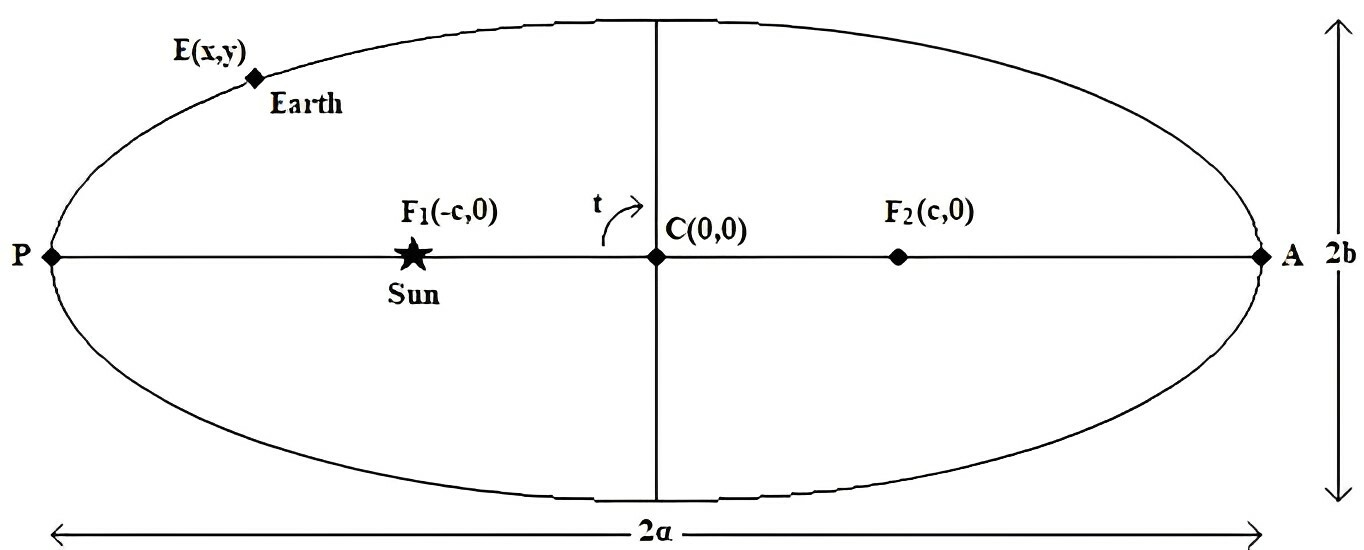
\includegraphics[width=0.9\textwidth]{Figures/Earths_orbit_updated.jpg}
    \caption{Η ελλειπτική τροχιά της Γης γύρω από τον Ήλιο.}
    \label{fig_Earths_orbit}
\end{figure}

Για την εκτίμηση της γωνίας $t$, θεωρήθηκε ότι η Γη απαιτεί 365 ημέρες για πλήρη περιστροφή \SI{360}{\degree}. 
Επομένως, για κάθε ημέρα του έτους, η Γη διασχίζει μία γωνία ίση με \SI{0,986}{\degree}, ενώ για κάθε περίοδο 10 λεπτών, 
που είναι και το επιθυμητό χρονικό βήμα σε αυτή τη μελέτη, η γωνία λαμβάνει τιμή ίση με \SI{0,986}{\degree\per144}, καθώς 
μία ημέρα αντιστοιχεί σε 144 χρονικά διαστήματα των 10 λεπτών. Τέλος, η παραμετρική εξίσωση που προκύπτει από τα παραπάνω 
και χρησιμοποιείται για τον υπολογισμό της απόστασης Γης-Ήλιου (απόσταση \english{F1E} στην Εικόνα \ref{fig_Earths_orbit}) 
για κάθε 10 λεπτά του έτους δίνεται από την Εξίσωση \ref{eq_r_dist}, η οποία με βάσει τις Εξισώσεις \ref{eq_x_param} και 
\ref{eq_y_param}, λαμβάνει την μορφή της Εξίσωσης \ref{eq_rt_dist}.

\begin{equation}
    \english{r(t') = \sqrt{\left[a \cdot \cos\left(\frac{0.986}{144} \cdot t'\right) - c\right]^2 + \left[b \cdot \sin\left(\frac{0.986}{144} \cdot t'\right)\right]^2}}
    \label{eq_rt_dist}
\end{equation}

\noindent όπου $r$ είναι η απόσταση Γης-Ήλιου για κάθε 10 λεπτά κατά την διάρκεια του έτους (\SI{}{\meter}), και 
$t'$ είναι ο δείκτης της περιόδου των 10 λεπτών (-) καθ’ όλη τη διάρκεια του έτους.

Στην Συνάρτηση 2 (\english{EarthSunDist}) του Παραρτήματος \ref{appx_A_4} – Κεφάλαιο 4, παρουσιάζονται τα κύρια σημεία του 
υπολογισμού της απόστασης Γης-Ήλιου, σύμφωνα με τις Εξισώσεις \ref{eq_ell_alpha} έως \ref{eq_ell_beta} και \ref{eq_rt_dist}.

Η υπολογιζόμενη απόσταση Γης-Ήλιου από τη Συνάρτηση 2 χρησιμοποιείται σε συνδυασμό με τις γωνίες \english{SZA} και 
\english{SAA}, που υπολογίζονται από τη Συνάρτηση 1, για την μετατροπή της θέσης του Ήλιου από σφαιρικές σε Καρτεσιανές 
συντεταγμένες, η οποία και παρουσιάζεται από τη Συνάρτηση 3 (\english{SunPosCart}) του Παραρτήματος 
\ref{appx_A_4} – Κεφάλαιο 4. Για τις χρονικές στιγμές στις οποίες η γωνία, που καθορίζει το ύψος του ήλιου και αναφέρεται ως 
συμπληρωματική γωνία της \english{SZA}, είναι μικρότερη από το μηδέν, περιγράφοντας έτσι τις νυχτερινές ώρες, οι 
συντεταγμένες για τη θέση του ήλιου δεν υφίστανται για την συγκεκριμένη εργασία.

\subsubsection{Συντεταγμένες του θερμοκηπίου στο Καρτεσιανό σύστημα συντεταγμένων}\label{subsub_greenhouse_coord}

Η τέταρτη συνάρτηση (Συνάρτηση 4) αφορά τη βάση ολόκληρης της μελέτης, το θερμοκήπιο. Η συγκεκριμένη συνάρτηση 
παρέχει τη δυνατότητα της χαρτογράφησης ενός αμφίρρικτου θερμοκηπίου και της εύρεσης των σημείων που το σχηματίζουν 
εντός ενός τρισδιάστατου Καρτεσιανού συστήματος συντεταγμένων. Ο προσανατολισμός του συστήματος 
(Ανατολή-Δύση-Βορράς-Νότος) προσδιορίστηκε με βάση τα αποτελέσματα της Συνάρτησης 1, όπου εκτιμάται η θέση του Ήλιου. 
Έτσι, η κατεύθυνση Βορρά-Νότου και η κατεύθυνση Ανατολής-Δύσης, αντιπροσωπεύονται από τον άξονα \english{x} και τον 
άξονα \english{y}, αντίστοιχα, ενώ το ύψος από την επιφάνεια αντιπροσωπεύεται από τον άξονα \english{z}. Η Συνάρτηση 
4 λαμβάνει ως εισόδους βασικές παραμέτρους που αφορούν μια βασική κατασκευαστική θερμοκηπιακή μονάδα, όπως ο 
προσανατολισμός (κατεύθυνση κορφιά), το πλάτος (μήκος μικρής πλευράς), το μήκος (μήκος μεγάλης πλευράς), καθώς και τα 
ύψη της υδρορροής και του κορφιά από την επιφάνεια του εδάφους. Ταυτόχρονα, λαμβάνεται υπόψη η επαναληψιμότητα της 
βασικής κατασκευαστικής μονάδας για τη δημιουργία του συνολικού θερμοκηπίου, είτε κατά μήκος είτε κατά πλάτος. Όλες 
οι μεταβλητές εισόδου της Συνάρτησης 4 παρουσιάζονται στον Πίνακα \ref{tab_fnc_4_inputs}.

\begin{table}[ht]
    \centering
    \caption{Χαρακτηριστικά θερμοκηπίου που χρησιμοποιούνται ως μεταβλητές εισόδου για την Συνάρτηση 4.}\label{tab_fnc_4_inputs} 
        \begin{tabular}{>{\centering\arraybackslash}m{7.5cm} >{\centering\arraybackslash}m{7.5cm}}
        \toprule
        \textbf{Στοιχείο θερμοκηπίου} & \textbf{Mεταβλητές eισόδου Συνάρτησης 4} \\
        \midrule
        Προσανατολισμός & \texttt{\english{dir}} \\
        Αριθμός κατασκευαστικών μονάδων – κατά πλάτος & \texttt{\english{numCU\_wdwise}} \\ 
        Αριθμός κατασκευαστικών μονάδων – κατά μήκος & \texttt{\english{numCU\_lnwise}} \\
        Πλάτος & \texttt{\english{grh\_width}} \\
        Μήκος & \texttt{\english{grh\_length}} \\ 
        Ύψος υδρορροής & \texttt{\english{gut\_hght}} \\
        Ύψος κορφιά & \texttt{\english{ridge\_hght}} \\
        \bottomrule
    \end{tabular}
\end{table}

Αρχικά, είναι απαραίτητο να καθοριστεί το σημείο αναφοράς, βάσει του οποίου θα σχηματιστεί το θερμοκήπιο. Αυτό θεωρείται 
ως η αρχή των αξόνων \english{(x,y,z)} = (0,0,0), η οποία αντιστοιχεί στην κάτω νοτιοδυτική γωνία του θερμοκηπίου. Με 
βάση αυτό το σημείο, ορίζονται όλα τα υπόλοιπα σημεία που αντιπροσωπεύουν τις άκρες του σκελετού της πρώτης 
κατασκευαστικής μονάδας του θερμοκηπίου. Αφού υπολογιστούν αυτά τα σημεία, αποθηκεύονται σε μια μεταβλητή δύο γραμμών 
τύπου “\english{cell}” στο \english{MATLAB}, με την πρώτη γραμμή να αντιστοιχεί στις θερμοκηπιακές μονάδες της περίπτωσης 
της κατά πλάτος επανάληψης, ενώ την δεύτερη να αντιστοιχεί στις θερμοκηπιακές μονάδες με βάση την περίπτωση της κατά 
μήκος επανάληψης. Οι διαστάσεις της μεταβλητής τύπου “\english{cell}” ποικίλλουν ανάλογα με τον αριθμό των κατασκευαστικών 
μονάδων. Τέλος, κάθε στοιχείο της μεταβλητής τύπου “\english{cell}” αποτελείται από έναν πίνακα τριών στηλών, μία για 
κάθε κατεύθυνση \english{(x,y,z)} και δέκα σειρές, μία για κάθε σημείο του θερμοκηπίου.

Η Συνάρτηση 4 (\english{GreenhouseCoord}) του Παραρτήματος \ref{appx_A_4} – Κεφάλαιο 4 περιέχει δύο περιορισμούς, ο πρώτος 
αφορά τον προσανατολισμό του κορφιά, για τον οποίο υπάρχουν μόνο δύο επιλογές, αυτή της κατεύθυνσης Ανατολής-Δύσης (Περίπτωση 1 – 
\english{Case} 1) και αυτή της κατεύθυνσης Βορρά-Νότου (Περίπτωση 2 – \english{Case} 2). Ο δεύτερος περιορισμός αφορά το 
γεγονός ότι ο αριθμός των κατασκευαστικών μονάδων πρέπει να είναι θετικός ακέραιος αριθμός, αλλά και στον ορισμό 
τουλάχιστον μίας κατασκευαστικής μονάδας. Για την ανίχνευση των σημείων του σκελετού του θερμοκηπίου, εκτός από τις δύο 
προαναφερθείσες περιπτώσεις, ήταν απαραίτητο να ορισθούν πρόσθετες υποπεριπτώσεις που να περιλαμβάνουν σενάρια για τον 
αριθμό των κατασκευαστικών μονάδων με επανάληψη κατά πλάτος ή κατά μήκος. Πιο συγκεκριμένα, οι περιπτώσεις αυτές 
περιγράφουν:

\begin{enumerate}
    \item Μία ή περισσότερες κατασκευαστικές μονάδες κατά πλάτος και καμία ή μία μονάδα κατά μήκος (Υποπερίπτωση 1). Η κατάσταση που αφορά την μία μονάδα κατά μήκος είναι ταυτόσημη με την πρώτη μονάδα κατά πλάτος. Ωστόσο, είναι απαραίτητο να οριστεί λόγω της διαφορετικής μεταβλητής στις μεταβλητές εισόδου της Συνάρτησης.
    \item Μία ή περισσότερες κατασκευαστικές μονάδες κατά μήκος και καμία ή μία μονάδα κατά πλάτος (Υποπερίπτωση 2).
    \item Περισσότερες από μία κατασκευαστικές μονάδες τόσο κατά πλάτος όσο και κατά μήκος (Υποπερίπτωση 3).
\end{enumerate}

Τέλος, δημιουργούνται τρεις διαφορετικοί πίνακες για τα σημεία, ένας για κάθε συντεταγμένη βάσει των χαρακτηριστικών 
παραμέτρων του θερμοκηπίου. Κάθε ένας από αυτούς αποτελείται από δέκα γραμμές, μία για κάθε σημείο, όντας η έξοδος 
(αποτέλεσμα) της ένθετης συνάρτησης \english{“GrhXYZ”}. Η χρήση αυτής της ένθετης συνάρτησης “συμπυκνώνει” και 
επιταχύνει τον κώδικα. Η επαναληψιμότητα των μονάδων για τις κατά πλάτος και κατά μήκος περιπτώσεις επιτυγχάνεται μέσω 
ενός βρόχου \english{“for”} για τις συντεταγμένες \english{x} και \english{y}, αντίστοιχα για κάθε υποπερίπτωση. Οι 
βρόχοι \english{“for”} για κάθε υποπερίπτωση παρουσιάζονται στον Πίνακα \ref{tab_alg_cases}. Αντίθετα, στην περίπτωση 
της κατεύθυνσης του κορφιά Βορρά-Νότου, η κατά πλάτος επανάληψη αφορά τη συντεταγμένη \english{y}, ενώ η κατά μήκος 
επανάληψη αφορά τη συντεταγμένη \english{x}. Η Συνάρτηση 4 παρουσιάζεται μόνο για την περίπτωση θερμοκηπίου 
προσανατολισμένου στην κατεύθυνση Ανατολής-Δύσης.

\begin{table}[ht]
    \centering
    \caption{Υποπεριπτώσεις για τον αριθμό των κατασκευαστικών μονάδων με κατά πλάτος ή κατά μήκος επανάληψη.}\label{tab_alg_cases} 
    \begin{tabular*}{\textwidth}{{@{\extracolsep\fill}c l l}}
        \toprule
        \textbf{Υποπερίπτωση} & \textbf{Κώδικας ορισμού} & \textbf{Κώδικας “\english{for loops}”} \\
        \midrule

        \multirow{3}{*}{\makecell{1}} 
        & \texttt{\english{numCU\_wdwise > 0 \&\& ...}} & \texttt{\english{for k=0:numCU\_wdwise-1}} \\ 
        & \texttt{\english{\ \ (numCU\_lnwise == 0 || ...}} & \texttt{\english{\ \ \ \ for l=0}} \\ 
        & \texttt{\english{\ \ numCU\_lnwise == 1)}} &  \\
        & \\

        \multirow{3}{*}{\makecell{2}} 
        & \texttt{\english{numCU\_lnwise > 0 \&\& ...}} & \texttt{\english{for k=0}} \\ 
        & \texttt{\english{\ \ (numCU\_wdwise == 0 || ...}} & \texttt{\english{\ \ \ \ for l=0:numCU\_lnwise-1}} \\ 
        & \texttt{\english{\ \ numCU\_wdwise == 1)}} &  \\
        & \\
        
        \multirow{2}{*}{\makecell{3}} 
        & \texttt{\english{numCU\_wdwise > 1 \&\& ...}} & \texttt{\english{for k=0:numCU\_wdwise-1}} \\ 
        & \texttt{\english{\ \ numCU\_lnwise > 1}} & \texttt{\english{\ \ \ \ for l=0:numCU\_lnwise-1}} \\ 
   
        \hline
        \end{tabular*}
\end{table}

\subsubsection{Υπολογισμός συντεταγμένων σκιάς}\label{subsub_shade_coord}

Τα σημεία που σχηματίζουν τη σκιασμένη από τα φωτοβολταϊκά επιφάνεια εντοπίζονται από τη Συνάρτηση 5. Για την εύρεση αυτής της 
επιφάνειας στο έδαφος, είναι απαραίτητο να βρεθούν τα σημεία που σχηματίζουν τα φωτοβολταϊκά στο τρισδιάστατο Καρτεσιανό σύστημα 
συντεταγμένων (\english{$x_{PV}$,$y_{PV}$,$z_{PV}$}), καθώς και το αντίστοιχο σημείο της θέσης του ήλιου 
(\english{$x_{sun}$,$y_{sun}$,$z_{sun}$}), όπως υπολογίζεται από τις Συναρτήσεις 1-3. Στο Τμήμα 1 του αλγορίθμου 
(\english{Calculation of PV Points}), που περιλαμβάνεται στο Παράρτημα \ref{appx_A_4} – Κεφάλαιο 4, υπολογίζονται τα σημεία της 
θέσης των φωτοβολταϊκών σύμφωνα με το Καρτεσιανό σύστημα συντεταγμένων.

Αρχικά, στο Τμήμα 1 του κώδικα, ορίζονται οι θέσεις των φωτοβολταϊκών που είναι εγκατεστημένα σε κάθε κατασκευαστική μονάδα. Με 
βάση το μήκος τόσο των φωτοβολταϊκών, όσο και του θερμοκηπίου, οι συνολικές διαθέσιμες θέσεις που μπορούν να λάβουν τα φωτοβολταϊκά 
στην οροφή του θερμοκηπίου είναι οκτώ. Εντούτοις, έχουν οριστεί κάποιοι περιορισμοί, βάσει των οποίων σταματά ο αλγόριθμος, δίνοντας 
αντίστοιχα μηνύματα σφάλματος. Οι περιορισμοί\- αυτοί αντιστοιχούν σε περιπτώσεις όπου το συνολικό μήκος της φωτοβολταϊκής συστοιχίας 
υπερβαίνει το συνολικό μήκος της οροφής του θερμοκηπίου (Περιορισμός 1), καθώς και σε περιπτώσεις όπου το πλάτος των φωτοβολταϊκών 
υπερβαίνει το μήκος του κεκλιμένου επιπέδου της οροφής (Περιορισμός 2). Ο κώδικας για τους συγκεκριμένους περιορισμούς 
παρουσιάζονται στον Πίνακα \ref{tab_PV_pos_limitations}.

\begin{table}[h]
    \centering
    \caption{Περιορισμοί για τις πιθανές θέσεις φωτοβολταϊκών.}\label{tab_PV_pos_limitations} 
    \begin{tabular*}{\textwidth}{{@{\extracolsep\fill}c l}}
        \toprule
        \textbf{Περιορισμός} & \textbf{Κώδικας ορισμού} \\
        \midrule
                
        \multirow{5}{*}{\makecell{1}} &
        \texttt{\english{if PV\_width > (sqrt((rigde\_hght-gut\_hght) .\textasciicircum2 + ...}} \\ &
        \texttt{\english{\ \ (grh\_width) .\textasciicircum2)) || PV\_width <= 0,}} \\ &
        \texttt{\english{\ \ \ \ error("The width of the PV Unit must be a positive ...}} \\ &
        \texttt{\english{\ \ \ \ \ \ integer and not exceed the length of the inclined ...}} \\ &
        \texttt{\english{\ \ \ \ \ \ plane of the roof"); end}} \\
        & \\
        
        \multirow{3}{*}{\makecell{2}} &
        \texttt{\english{if grh\_length < numel(pos\_PV(n)) * PV\_length,}} \\ & 
        \texttt{\english{\ \ \ \ error("The PV units exceed the limits of the ...}} \\ &
        \texttt{\english{\ \ \ \ \ \ greenhouse roof"); end}} \\
                
        \hline
    \end{tabular*}
\end{table}

Παράλληλα, στο Τμήμα 1 του κώδικα διακρίνονται δύο ακόμη περιπτώσεις, η μία για την τοποθέτηση των φωτοβολταϊκών σε θερμοκήπιο με 
κατεύθυνση Ανατολής-Δύσης και η άλλη για την τοποθέτηση των φωτοβολταϊκών σε θερμοκήπιο με κατεύθυνση Βορρά-Νότου. Αυτές οι 
περιπτώσεις διαχωρίζονται λόγω της επανάληψης που απαιτείται για την εύρεση των συντεταγμένων των φωτοβολταϊκών. Στην πρώτη 
περίπτωση, απαιτείται επανάληψη για τη συντεταγμένη \english{x}, καθώς είναι αυτή που διαφέρει μεταξύ των κατασκευαστικών μονάδων, 
λόγω της επανάληψης παράλληλα στον άξονα \english{x}. Ταυτόχρονα, με την τοποθέτηση των φωτοβολταϊκών να γίνεται με τη μεγάλη 
πλευρά τους παράλληλα προς τον κορφιά, αλλάζει η συντεταγμένη \english{y}, με την τιμή της να υπολογίζεται μέσω επανάληψης με 
βάση το μήκος του φωτοβολταϊκού και τη θέση όπου τοποθετείται κάθε φωτοβολταϊκό. Η συντεταγμένη \english{y} για την περίπτωση των 
διαφορετικών μονάδων στην περίπτωση της κατεύθυνσης Ανατολής-Δύσης παραμένει σταθερή. Για τη δεύτερη περίπτωση, με το θερμοκήπιο να 
έχει κατεύθυνση Βορρά-Νότου, η συντεταγμένη \english{y} λειτουργεί όπως η συντεταγμένη \english{x} της προηγούμενης περίπτωσης, με 
αυτή να μεταβάλλεται μεταξύ των κατασκευαστικών μονάδων, καθώς τώρα αυτές επαναλαμβάνονται παράλληλα με τον άξονα \english{y}. Κατά 
συνέπεια, η τιμή της συντεταγμένης \english{x} υπολογίζεται μέσω επανάληψης με βάση το μήκος και τη θέση του φωτοβολταϊκού.

Με τα φωτοβολταϊκά στην οροφή του θερμοκηπίου τοποθετημένα έτσι ώστε η μεγάλη τους πλευρά να είναι ίδια με τον κορφιά, μερικά από 
τα σημεία τους είναι ίδια με τα ήδη υπολογισμένα σημεία του θερμοκηπίου. Οι συντεταγμένες των υπόλοιπων σημείων έχουν βρεθεί με βάση 
απλές γεωμετρικές σχέσεις και τα χαρακτηριστικά του θερμοκηπίου. Τέλος, η συντεταγμένη \english{z} εμφανίζεται η ίδια τόσο για την 
πρώτη όσο και για τη δεύτερη περίπτωση, καθώς τόσο η υδρορροή όσο και το ύψος του κορφιά παραμένουν σταθερά.

Στο Τμήμα 1, ο κώδικας παρουσιάζεται μόνο για την περίπτωση θερμοκηπίου με προσανατολισμό Ανατολής-Δύσης. Για την τρισδιάστατη 
οπτικοποίηση των φωτοβολταϊκών στην οροφή του θερμοκηπίου, είναι απαραίτητο να δημιουργηθούν πλέγματα δεδομένων με βάση τα σημεία 
που παρουσιάζονται οι γωνίες του κάθε φωτοβολταϊκού. Οι κύριες εντολές που χρησιμοποιούνται είναι “\texttt{\english{linspace}}” 
και “\texttt{\english{meshgrid}}”, ενώ η μεταβλητή “\texttt{\english{CU\_tables}}” είναι ένας πίνακας τύπου “\english{cell}” που 
περιέχει τα σημεία του θερμοκηπίου που έχουν εξαχθεί από τη Συνάρτηση 4. Με βάση τα σημεία που σχετίζονται με τις τέσσερις γωνίες 
του φωτοβολταϊκού πλαισίου και το σημείο που σχετίζεται με τη θέση του ήλιου, σχηματίζονται τέσσερις ευθείες για κάθε φωτοβολταϊκό 
πλαίσιο. Κάθε μία από αυτές τις ευθείες που σχηματίζονται για κάθε επιθυμητή χρονική στιγμή \english{t} αντιστοιχεί σε ένα από τα 
τέσσερα σημεία του φωτοβολταϊκού, ενώ κοινό σημείο είναι η θέση του ήλιου. Για κάθε μία από αυτές τις τέσσερις ευθείες, υπάρχει ένα 
τρισδιάστατο διάνυσμα της μορφής (Εξίσωση \ref{eq_r_sh_vector}):

\begin{multline}
    \english{\vec{r}_{sh.point,n} = \left(\vec{x}_{sh,n}, \vec{y}_{sh,n}, \vec{z}_{sh,n} \right) =} \\
    \english{= \left[ x_n + k \cdot (x_s - x_n), y_n + k \cdot (y_s - y_n), z_n + k \cdot (z_s - z_n) \right]}
    \label{eq_r_sh_vector}
\end{multline}

\noindent όπου \english{$\vec{r}_{sh.point,n}$} είναι το διάνυσμα θέσης του σημείου σκίασης που προέρχεται από ένα από τα τέσσερα 
σημεία του φωτοβολταϊκού, \english{$\vec{x}_{sh,n}$, $\vec{y}_{sh,n}$, $\vec{z}_{sh,n}$} είναι τα διανύσματα θέσης του σημείου 
σκίασης ως προς κάθε άξονα του τρισδιάστατου συστήματος συντεταγμένων, \english{$x_s$, $y_s$} και \english{$z_s$} είναι οι 
συντεταγμένες που ορίζουν τη θέση του ήλιου, \english{$x_n$, $y_n$} και \english{$z_n$}, είναι οι συντεταγμένες που ορίζουν κάθε 
σημείο του φωτοβολταϊκού, με $n$ = 1, 2, 3, 4, και $k$ είναι μια σταθερά.

Από την Εξίσωση \ref{eq_r_sh_vector}, λαμβάνεται ένα σύστημα τριών μερικών εξισώσεων που αντιπροσωπεύουν τις συντεταγμένες των 
σημείων που σχηματίζουν τη σκιά (Εξίσωση \ref{eq_x_sh_vector}, \ref{eq_y_sh_vector} και \ref{eq_z_sh_vector}).

\begin{equation}
    \english{x_{sh,n}(k) = x_{n} + k \cdot (x_s - x_n)}
    \label{eq_x_sh_vector}
\end{equation}

\begin{equation}
    \english{y_{sh,n}(k) = y_{n} + k \cdot (y_s - y_n)}
    \label{eq_y_sh_vector}
\end{equation}

\begin{equation}
    \english{z_{sh,n}(k) = z_{n} + k \cdot (z_s - z_n)}
    \label{eq_z_sh_vector}
\end{equation}

Επιλύοντας το παραπάνω σύστημα εξισώσεων και ορίζοντας τη συντεταγμένη \english{z} ($z_{sh}$) ίση με 0, δεδομένου ότι η σκιά 
βρίσκεται στο έδαφος (\english{xy}-επίπεδο στο τρισδιάστατο σύστημα συντεταγμένων), λαμβάνονται δύο εξισώσεις, μία για τις τιμές 
της συντεταγμένης \english{x} της σκιάς και μία για τις τιμές της συντεταγμένης \english{y} (Εξισώσεις \ref{eq_x_shadow} και 
\ref{eq_y_shadow}, αντίστοιχα).

\begin{equation}
    \english{x_{sh} = x_n - c_n \cdot z_n}
    \label{eq_x_shadow}
\end{equation}

\begin{equation}
    \english{y_{sh} = y_n - \frac{z_n}{b_n}}
    \label{eq_y_shadow}
\end{equation}

\noindent όπου $b_n$ και $c_n$ δίνονται από τις Εξισώσεις \ref{eq_b_n} και \ref{eq_c_n}, αντίστοιχα.

\begin{equation}
    \english{b_n = \frac{z_s - z_n}{y_s - y_n}}
    \label{eq_b_n}
\end{equation}

\begin{equation}
    \english{c_n = \frac{x_s - x_n}{z_s - z_n}}
    \label{eq_c_n}
\end{equation}

Η Συνάρτηση 5 (\english{PVShadowPoint}) του Παραρτήματος \ref{appx_A_4} – Κεφάλαιο 4 παρέχει τους υπολογισμούς των σημείων της 
σκιάς, σύμφωνα με τις Εξισώσεις \ref{eq_x_shadow} έως \ref{eq_c_n}.

\subsubsection{Δυαδική ανάλυση}\label{subsub_binary_analysis}

Για την αναπαράσταση της περιοχής που καλύπτεται από το θερμοκήπιο έχουν δημιουργηθεί πίνακες με λογικές τιμές (0 και 1). Όσον 
αφορά το θερμοκήπιο, η τιμή 0 (ψευδής – \english{false}) αντιστοιχεί σε μια περιοχή που δεν καλύπτεται από θερμοκήπιο, ενώ η 
τιμή 1 (αληθής – \english{true}) αναφέρεται σε μια περιοχή που περικλείεται από τα όρια του θερμοκηπίου. Λόγω της φύσης του 
ζητήματος, αυτός ο πίνακας θα είναι πάντα ο ίδιος για κάθε περίοδο του έτους. Όσον αφορά τη σκιά που σχηματίζουν τα φωτοβολταϊκά, 
ο αντίστοιχος πίνακας θα έχει τις ίδιες διαστάσεις με τον αντίστοιχο πίνακα του θερμοκηπίου. Αυτό συμβαίνει επειδή ο αλγόριθμος 
εκτιμά τη σκιά στο καλυπτόμενο από το θερμοκήπιο έδαφος σε σχέση με το συνολικό έδαφος που καλύπτεται από το θερμοκήπιο, και όχι 
σε ολόκληρη την επιφάνεια. Όπως και πριν, οι τιμές 0 και 1 αντιπροσωπεύουν τις μη σκιασμένες και σκιασμένες περιοχές, αντίστοιχα.

Αρχικά δημιουργείται ένας πίνακας μηδενικών τιμών (\english{false}) με βάση τις διαστάσεις που εισάγονται για το θερμοκήπιο. Πιο 
συγκεκριμένα, θεωρείται ότι οι σειρές του πίνακα αντιστοιχούν στις τιμές της \english{y}-συνιστώσας των συντεταγμένων θερμοκηπίου, 
ενώ οι στήλες του πίνακα αντιστοιχούν στις τιμές της \english{x}-συνιστώσας. Λόγω της ανάγκης έκφρασης των διαστάσεων του 
θερμοκηπίου με ακέραιες τιμές (δεδομένου ότι κάθε στήλη-σειρά αντιστοιχεί σε ένα συγκεκριμένο σημείο του επιπέδου \english{x-y} 
του Καρτεσιανού συστήματος συντεταγμένων) και δεδομένου ότι η ακρίβεια των εισαγόμενων τιμών (μήκος του θερμοκηπίου, πλάτος του 
θερμοκηπίου κ.λπ.) είναι της τάξης των εκατόμετρων (μέχρι δύο δεκαδικά ψηφία), όλες οι διαστάσεις, τόσο για το θερμοκήπιο όσο και 
για την σκιά, μετατρέπονται από μέτρα σε εκατοστόμετρα. Ένας άλλος μετασχηματισμός των πραγματικών σημείων του θερμοκηπίου, αλλά 
και της σκιάς, είναι η επιπλέον αύξηση κάθε τιμής κατά \SI{1}{\centi\meter} αφού δεν υπάρχουν μηδενικές στήλες ή σειρές στον 
δημιουργημένο πίνακα. Τέλος, με το υπολογισμό των ορίων του θερμοκηπίου από την Συνάρτηση 4, τα κελιά του πίνακα που αντιστοιχούν 
σε τιμές εντός των ορίων του θερμοκηπίου αντικαθίστανται με την τιμή 1 (αληθές). Παράλληλα, θα πρέπει να σημειωθεί ότι η τιμή 1 
αφορά μόνο την καλλιεργήσιμη μονάδα του θερμοκηπίου (Κατασκευαστική Μονάδα 2 – \english{Construction Unit 2 – CU 2}) και όχι 
ολόκληρο το θερμοκήπιο. Ο κώδικας που εφαρμόζεται για τα ανωτέρω παρουσιάζεται στο Τμήμα του κώδικα 2Α του Παραρτήματος 
\ref{appx_A_4} – Κεφάλαιο 4.

Όσον αφορά τη σκιά που σχηματίζουν τα φωτοβολταϊκά, ακολουθείται η ίδια στρατηγική με κάποια επιπλέον απαραίτητα σημεία. Το πρώτο 
σημείο αφορά τη μετατροπή όλων των συντεταγμένων των ορίων της σκιάς σε θετικές ποσότητες. Θεωρώντας ένα σύστημα συντεταγμένων 
στο οποίο οι συντεταγμένες της θέσης του ήλιου λαμβάνουν είτε θετικές είτε αρνητικές τιμές, οι συντεταγμένες κάθε σημείου σκιάς 
μπορεί να είναι επίσης είτε θετικές είτε αρνητικές, αντίστοιχα. Ωστόσο, ένας πίνακας, όπου κάθε γραμμή-στήλη αντιστοιχεί σε ένα 
σημείο του επιπέδου \english{x-y}, απαιτεί κάθε τιμή να είναι θετική και μη μηδενική. Έτσι, κάθε μη θετική συντεταγμένη της σκιάς 
μετατρέπεται σε 1. Τα όρια της σκιάς γίνονται στενότερα, χωρίς ωστόσο να επηρεάζεται το τελικό επιθυμητό αποτέλεσμα καθώς τα όρια 
του θερμοκηπίου αποτελούνται αποκλειστικά από θετικές τιμές και σκοπός του αλγορίθμου είναι ο υπολογισμός της σκίασης μέσα σε αυτό. 
Τέλος, για την καλύτερη απόδοση του αλγορίθμου, τα όρια της σκιάς που παρουσιάζουν θετικές τιμές και είναι μεγαλύτερα από τα όρια 
του θερμοκηπίου εξισώνονται με αυτά των ορίων του θερμοκηπίου χωρίς να επηρεάζεται και πάλι το τελικό αποτέλεσμα το οποίο, όπως 
προαναφέρθηκε, είναι η εκτίμηση της σκιάς μέσα στο θερμοκήπιο και σε σχέση με τη συνολική επιφάνεια αυτού. Τα πρόσθετα αναγκαία 
σημεία του κώδικα που εφαρμόζονται για τα ανωτέρω παρουσιάζονται στο Τμήμα του κώδικα 2Β του Παραρτήματος 
\ref{appx_A_4} – Κεφάλαιο 4.

\subsubsection{Υπολογισμός της σκιασμένης επιφάνειας στο θερμοκήπιο}\label{subsub_shaded_surf_calc}

Όπως έχει προαναφερθεί, το τελικό επιθυμητό αποτέλεσμα που εξάγεται από τον αλγόριθμο αφορά την επιφάνεια της καλλιεργήσιμης 
μονάδας του θερμοκηπίου που καλύπτεται από τη σκιά των φωτοβολταϊκών. Δημιουργώντας πίνακες λογικών τιμών από τα προηγούμενα 
βήματα, υπάρχει η δυνατότητα να γνωρίζουμε εάν κάθε τετραγωνικό εκατοστό της επιφάνειας του θερμοκηπίου καλύπτεται επίσης από τη 
σκιά. Η βασική ιδέα είναι ότι δεδομένου ότι ο αριθμός των κελιών των πινάκων “\texttt{\english{binary\_array\_CU\_2}}” και 
“\texttt{\english{binary\_array\_shade}}” είναι ίδιος και κάθε κελί αντιπροσωπεύει το ίδιο τετραγωνικό εκατοστό της επιφάνειας, 
τότε ο αριθμός των κελιών του “\texttt{\english{binary\_array\_CU\_2}}” που βρίσκονται στην ίδια θέση με τα κελιά του 
“\texttt{\english{binary\_array\_shade}}” θα περιέχουν και τα δύο την λογική τιμή 1 (αληθής),  αντιπροσωπεύοντας το μέγεθος της 
σκιασμένης περιοχής του θερμοκηπίου σε \SI{}{\centi\meter\squared}. Τέλος, διαιρώντας με τον συνολικό αριθμό κελιών του πίνακα 
“\texttt{\english{binary\_array\_CU\_2}}” που περιέχει την τιμή 1, υπολογίζεται το ποσοστό της σκιασμένης περιοχής. Τα ανωτέρω 
περιγράφονται στο Τμήμα 3 του κώδικα, το οποίο περιέχεται στο Παράρτημα \ref{appx_A_4} – Κεφάλαιο 4., με τον πολλαπλασιασμό επί 
$10^{-4}$ να αφορά τη μετατροπή από \SI{}{\centi\meter\squared} σε \SI{}{\meter\squared}.

\subsubsection{Διερεύνηση σκιασμένων σημείων}\label{subsub_shaded_point_inv}

Προκειμένου να ελεγχθεί εάν ένα σημείο εντός του θερμοκηπίου σκιάζεται από τα φωτοβολταϊκά ή όχι, οι συντεταγμένες του 
χρησιμοποιούνται ως τιμές εισόδου στον αλγόριθμο. Έτσι, γίνεται εφικτή η αναλυτική χαρτογράφηση της σκιασμένης περιοχής 
για κάθε επιθυμητή χρονική περίοδο. Οι τιμές των συντεταγμένων πρέπει να εισαχθούν σε ζευγάρια (\english{x,y}), καθώς κανένα 
σημείο δεν ορίζεται προσθέτοντας μόνο την \english{x}- ή την \english{y}-συντεταγμένη, ενώ σε περίπτωση που εισαχθεί μόνο η 
\english{x}- ή η \english{y}-συντεταγμένη, ο αλγόριθμος σταματά δίνοντας την αντίστοιχη ένδειξη σφάλματος. Εάν ο χρήστης δεν 
επιθυμεί την εκτέλεση της παραπάνω λειτουργίας, ο αλγόριθμος σταματά, αφού πρώτα εξάγει όλα τα προηγούμενα αποτελέματα.

Η έξοδος της συγκεκριμένης συνάρτησης είναι ένας πίνακας για κάθε σημείο, με τιμές 0 και 1 για τις περιπτώσεις μη σκιασμένων 
και σκιασμένων σημείων, αντίστοιχα. Κάθε πίνακας αποτελείται από έναν μεταβλητό αριθμό σειρών ανάλογα με τις χρονικές στιγμές 
που εκτελείται ο αλγόριθμος και έναν μεταβλητό αριθμό στηλών, ανάλογα με τον αριθμό των φωτοβολταϊκών συστυχιών. Για χρονικές 
περιόδους κατά την διάρκεια της νύχτας, η έξοδος λαμβάνει τιμές \english{NaN} (μη διαθέσιμες τιμές). Τα ανωτέρω περιγράφονται 
στο Τμήμα 4 του κώδικα, το οποίο περιέχεται στο Παράρτημα \ref{appx_A_4} – Κεφάλαιο 4..

\subsubsection{Πλήρης αλγόριθμος}\label{subsub_comlete_alg}

Όπως αναφέρθηκε παραπάνω, ο αλγόριθμος αποτελείται από πέντε διακριτές συναρτήσεις και τέσσερα μεμονωμένα τμήματα. Για την 
εξαγωγή των αποτελεσμάτων του αλγορίθμου, ως τιμές εισόδου για την κάθε επόμενη συνάρτηση ή τμήμα του κώδικα, χρησιμοποιούνται 
οι τιμές εξόδου της προηγούμενης συνάρτησης. Εισάγοντας τις επιθυμητές τιμές για το χρόνο (έτος, μήνας, ημέρα, ώρα, λεπτά, 
δευτερόλεπτα, ζώνη ώρας), για το θερμοκήπιο (προσανατολισμός, αριθμός κατασκευαστικών μονάδων κατά πλάτος και κατά μήκος, πλάτος 
και μήκος κατασκευαστικής μονάδας, ύψος υδρορροής και κορφιά), για τις γεωγραφικές συντεταγμένες (γεωγραφικό πλάτος και μήκος της 
θέσης του θερμοκηπίου), για τις διαστάσεις των φωτοβολταϊκών (μήκος και πλάτος),  και τέλος, για την τοποθέτηση των φωτοβολταϊκών 
στη στέγη, υπάρχει η δυνατότητα, με βάση τον τρόπο διαμόρφωσης του αλγορίθμου, να εξαχθεί η επιφάνεια (\SI{}{\meter\squared}) που 
καλύπτεται από την σκιά των φωτοβολταϊκών εντός της καλλιεργήσιμης μονάδας του θερμοκηπίου με ακρίβεια δύο δεκαδικών ψηφίων, το 
ποσοστό της σκιασμένης επιφάνειας σε σχέση με τη συνολική επιφάνεια της μονάδας (\SI{}{\percent}), και τέλος δύο αντιπροσωπευτικά 
γραφικά, ένα δισδιάστατο και ένα τρισδιάστατο. Ο πλήρης αλγόριθμος (\english{PVShading}) παρουσιάζεται στο Παράρτημα 
\ref{appx_A_4} – Κεφάλαιο 4.

\subsubsection{Μέθοδος επικύρωσης του αλγορίθμου}\label{subsub_validation}

Όπως έχει αναφερθεί στην Παράγραφο \ref{sub_PVs}, oι φωτοβολταϊκές μονάδες που έχουν ενσωματωθεί στην οροφή του πειραματικού 
θερμοκηπίου είναι ημιδιαφανείς, με τη σκίαση που παρουσιάζουν στην επιφάνεια του εδάφους να ανέρχεται στο $\sim$\SI{51}{\percent} 
της συνολικής τους επιφάνειας. Το γεγονός αυτό, σε συνδυασμό με την ικανότητά τους να διασκορπίζουν το προσπίπτον σε αυτά φως, 
καθιστά τη μελέτη της ακτινοβολίας που τα διαπερνά και, κατά συνέπεια, της σκίασης ιδιαίτερα δύσκολη.

Προκειμένου να πραγματοποιηθεί η επικύρωση του αλγορίθμου, και ταυτόχρονα λαμβάνοντας υπόψη ότι η λειτουργία του αλγορίθμου 
βασίζεται στο γεγονός ότι τα ενσωματωμένα στην οροφή του θερμοκηπίου φωτοβολταϊκά είναι αδιαφανή, ήταν απαραίτητο να προστεθεί 
ένα αδιαφανές μέσο για την κάλυψή τους. Το αδιαφανές μέσο που χρησιμοποιήθηκε ήταν ένα χαρτόνι πάχους περίπου \SI{4}{\milli\meter}, 
ενώ η τοποθέτησή του έγινε κάτω από την επιφάνεια των φωτοβολταϊκών εντός του θερμοκηπίου, και κατά μήκος της επιφάνειάς τους, όπως 
φαίνεται στην Εικόνα \ref{fig_opaque_cover}. Αποτέλεσμα της χρήσης αυτού του μέσου είναι η δημιουργία έντονης σκίασης, παρόμοιας 
με αυτή που δημιουργείται από τα αδιαφανή φωτοβολταϊκά, και ως εκ τούτου, η ανίχνευση διαφορών στην ακτινοβολία που καταγράφεται 
από δύο πυρανόμετρα τοποθετημένα εντός του θερμοκηπίου.

Όσον αφορά την καταγραφή της \english{GHI} (\SI{}{\watt\per\meter\squared}), χρησιμοποιήθηκαν δύο πυρανόμετρα \english{CMP3} 
της εταιρείας \english{Kipp \& Zonen} (για περισσότερες πληροφορίες βλ. Παράγραφο \ref{sub_eksoplismos}), τα οποία τοποθετήθηκαν 
στο ύψος της επιφάνειας, καθώς η θέση της σκίασης που υπολογίστηκε με βάση τον αλγόριθμο αφορά το συγκεκριμένο ύψος. Τα 
δεδομένα που χρησιμοποιήθηκαν για την επικύρωση του αλγορίθμου αφορούν την περίοδο από 05/08/2023 έως 29/08/2023. Κατά τη 
διάρκεια αυτής της περιόδου, η θέση του πρώτου πυρανόμετρου (Πυρανόμετρο 1) είχε συντεταγμένες 
(\english{$x_{P,1}$,$y_{P,1}$}) = (4.81,11.85), ενώ η θέση του δεύτερου (Πυρανόμετρο 2) είχε συντεταγμένες 
(\english{$x_{P,2}$,$y_{P,2}$}) = (4.81,4.55) (Εικόνα \ref{fig_pyranometers_pos}). Οι τιμές αυτές αναφέρονται σε 
αποστάσεις (\SI{}{\meter}) από την αρχή των αξόνων, όπως ορίζονται με βάση τον αλγόριθμο. Τέλος, τα δεδομένα ακτινοβολίας 
λαμβάνονται με χρονικό βήμα 10 λεπτών, με την τιμή που καταγράφεται κάθε φορά να είναι ο μέσος όρος μονόλεπτων δεδομένων. 
Εκτός από τα δύο πυρανόμετρα μέσα στο θερμοκήπιο, ένα άλλο πυρανόμετρο \english{CMP3} βρίσκεται έξω από το θερμοκήπιο για την 
παρακολούθηση της ακτινοβολίας πριν αυτή διεισδύσει στο θερμοκήπιο. Οι μετρήσεις από αυτό το πυρανόμετρο λαμβάνονται με τον ίδιο 
τρόπο όπως και οι προηγούμενες.

\begin{figure}[ht]%
    \centering
    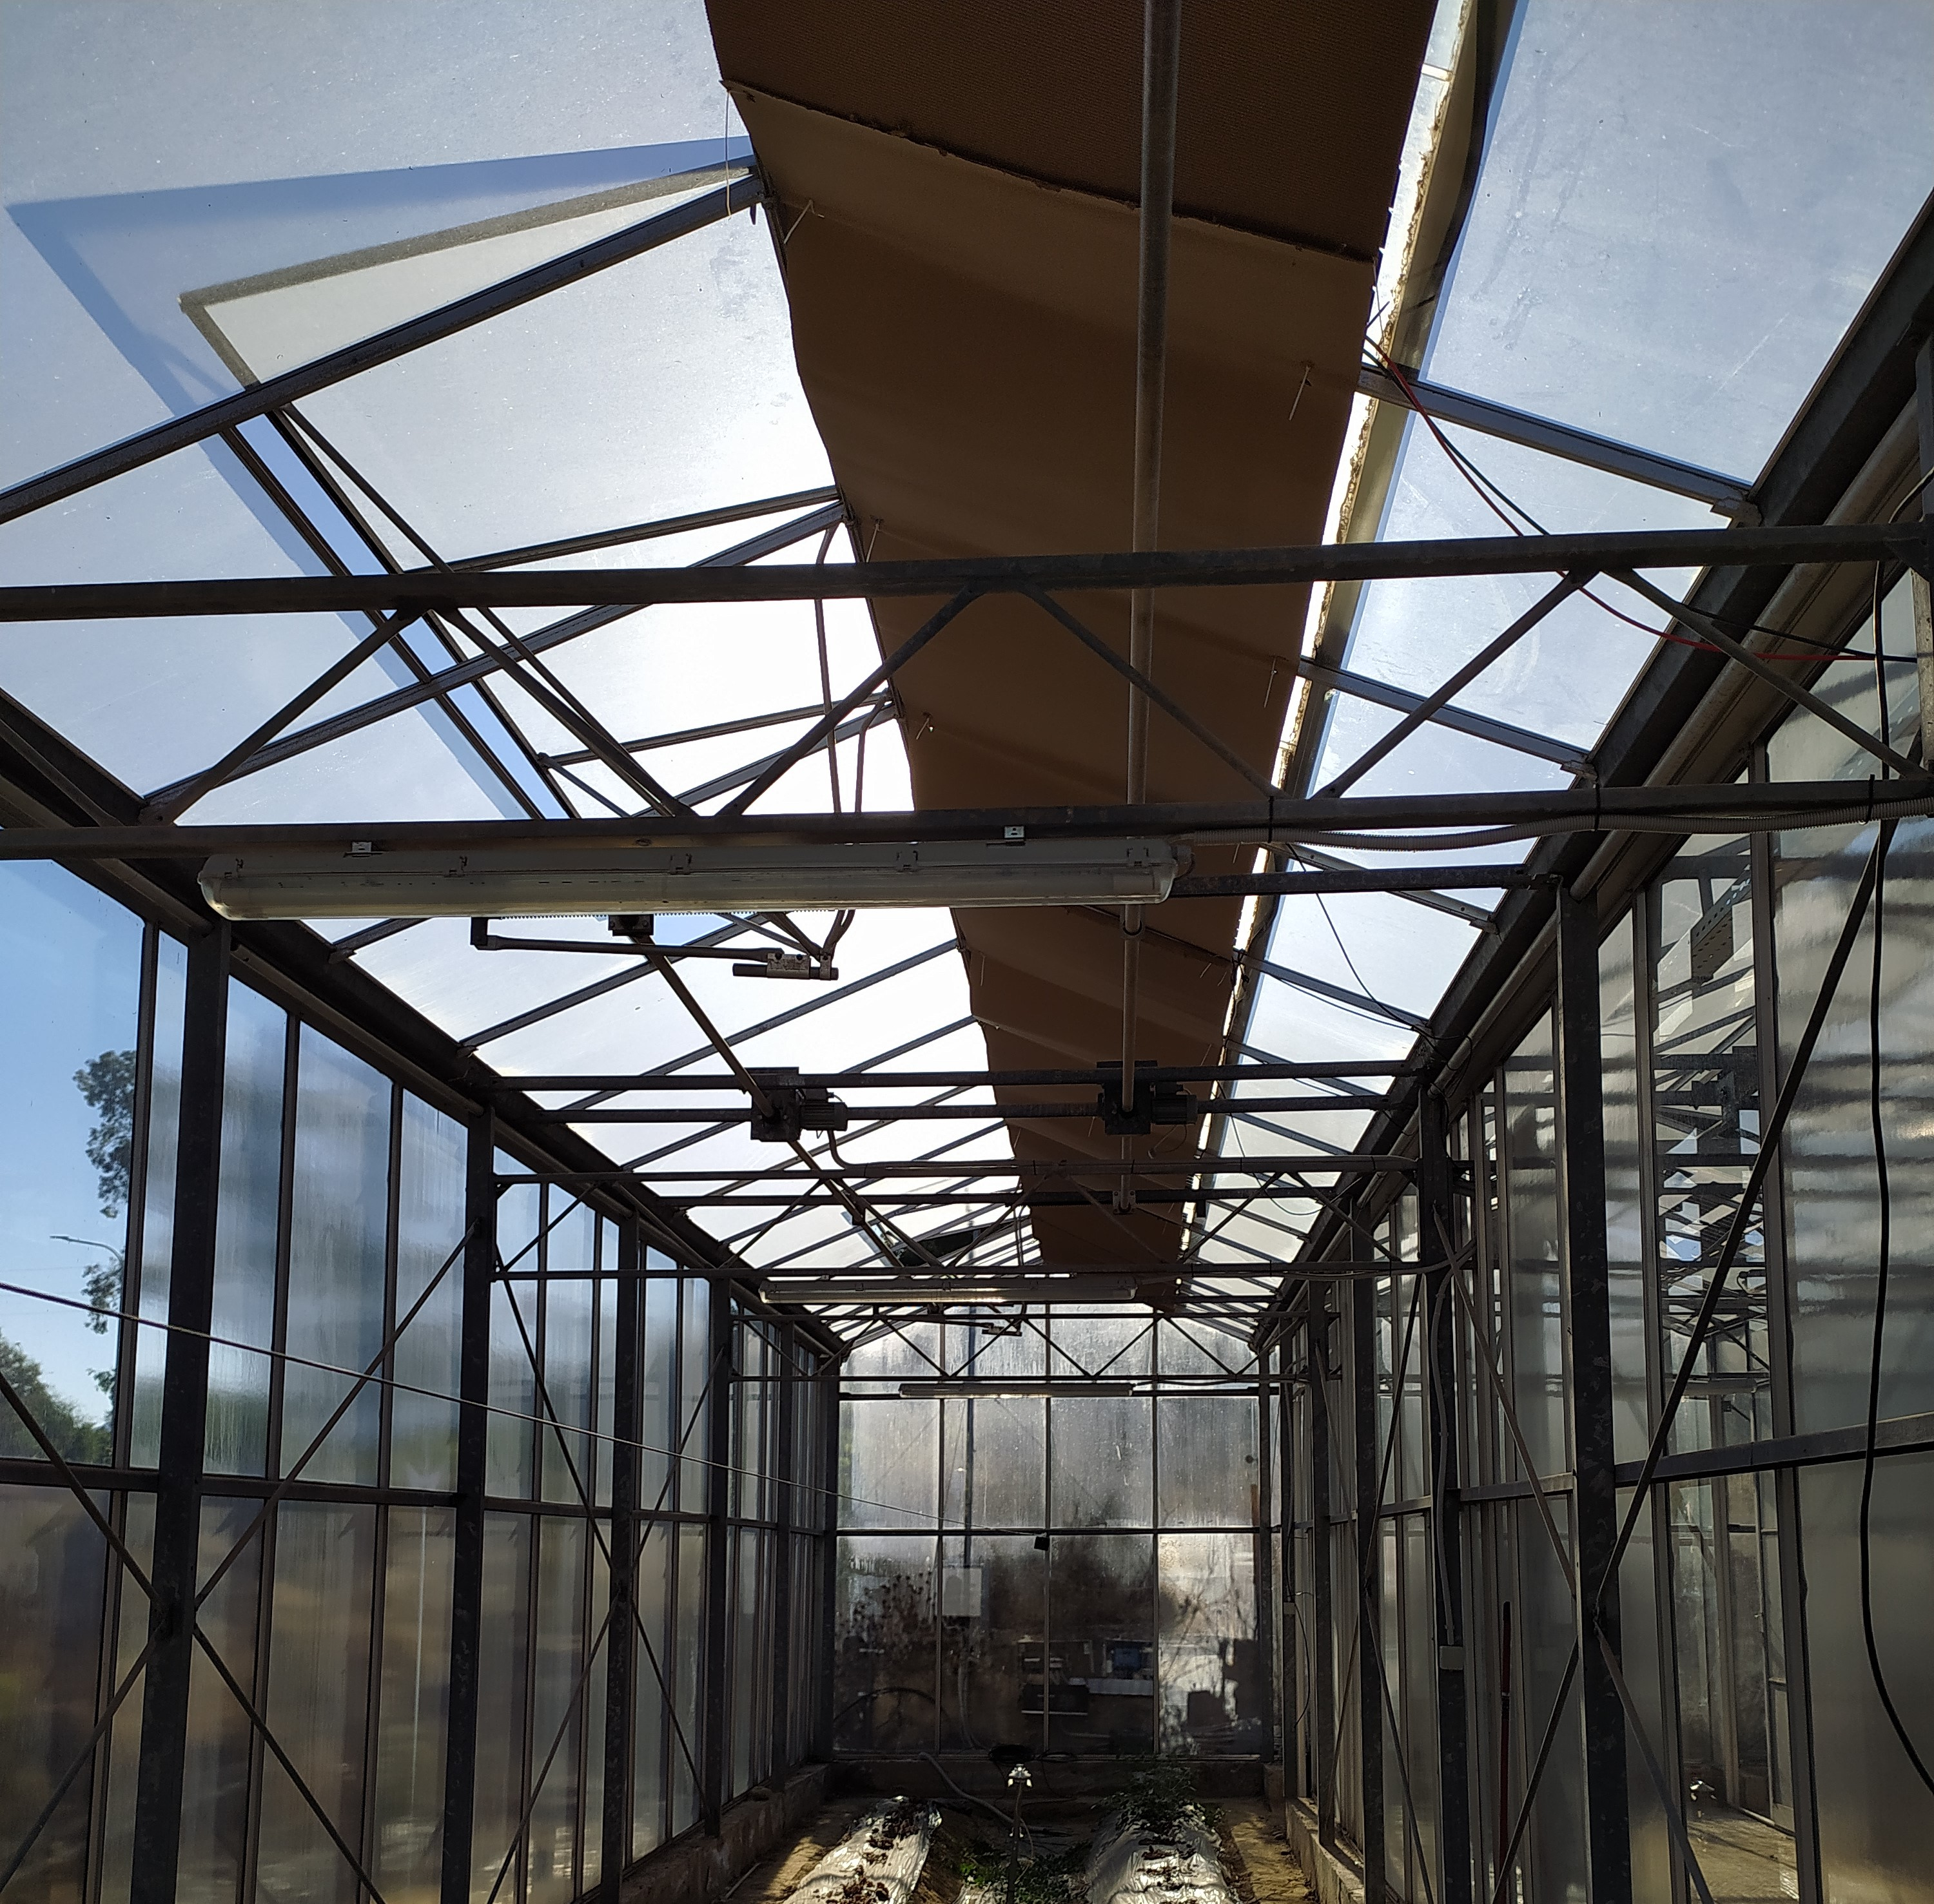
\includegraphics[scale=0.08]{Figures/opaque_cover.jpg}
    \caption{Φωτοβολταϊκά πλαίσια καλυμμένα από αδιαφανές υλικό.}
    \label{fig_opaque_cover}
\end{figure}

\begin{figure}[ht]%
    \centering
    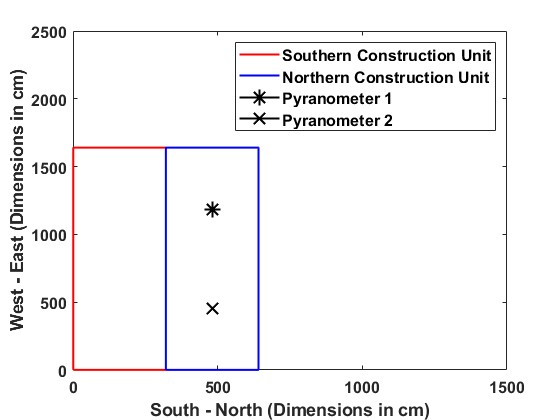
\includegraphics[scale=0.55]{Figures/pyranometers_pos.jpg}
    \caption{Θέσεις των πυρανόμετρων μέσα στο θερμοκήπιο.}
    \label{fig_pyranometers_pos}
\end{figure}

Ο συντελεστής που χρησιμοποιήθηκε σε αυτή την εργασία είναι ο Συντελεστής Μεταβλητότητας (\english{Coefficient of Variation – CV}). 
Ο συντελεστής μεταβλητότητας ορίζεται τόσο στη στατιστική όσο και στη θεωρία πιθανοτήτων ως ο λόγος μεταξύ της τυπικής απόκλισης 
και της μέσης τιμής, ενώ επιτρέπει την ανίχνευση διαφόρων μεταβολών. Η τιμή του \english{CV} υπολογίζεται συνήθως ως ποσοστό, ενώ 
σε σύγκριση με ένα μεγαλύτερο \english{CV} \lcitep{algorithm_bib23}, μια χαμηλότερη τιμή του δείχνει μικρότερη μεταβλητότητα στα 
δεδομένα \lcitep{algorithm_bib22,algorithm_bib24}.

Στην εργασία αυτή βρέθηκαν οι χρονικές περίοδοι κατά τις οποίες το πυρανόμετρο σκιάζεται από τα φωτοβολταϊκά, μετά την εκτέλεση 
του αλγορίθμου για κάθε χρονικό διάστημα 10 λεπτών της υπό μελέτη ημέρας. Οι μεταβολές της ακτινοβολίας για τα καθορισμένα 
διαστήματα αποθηκεύονται, δημιουργώντας ένα σύνολο δεδομένων $S_i$, όπου $i$ είναι ο αριθμός της ημέρας. Στη συνέχεια, για 
κάθε ημέρα και μόνο για τις ώρες κατά την διάρκεια της ημέρας, δημιουργήθηκαν πενήντα ξεχωριστά και τυχαία σύνολα δεδομένων 
μεταβολής της ακτινοβολίας ($U_{i,1}$ έως $U_{i,50}$) σχετικά με το πυρανόμετρο ενώ δεν είναι σκιασμένο και του οποίου το μέγεθος 
είναι ίσο με το μέγεθος του $S_i$. Ο μεγάλος αριθμός τυχαίων συνόλων δεδομένων στοχεύει στη χρήση των τιμών για κάθε χρονική 
στιγμή. Τέλος, υπολογίστηκε ο συντελεστής μεταβλητότητας, τόσο για το $S_i$ όσο και για το $U_{i,1}$ έως $U_{i,50}$. Μια μικρή 
τιμή του συντελεστή μεταβλητότητας για το πακέτο δεδομένων $S$, σε σύγκριση με τις αντίστοιχες τιμές του συντελεστή για τα σύνολα 
δεδομένων $U_{i,1}$ έως $U_{i,50}$, υποδηλώνει την ομοιομορφία της μεταβολής ακτινοβολίας στην περιοχή που σκιάζεται από τα 
φωτοβολταϊκά, δεδομένου ότι ένα σημείο παραμένει μέσα σε αυτό για μεγαλύτερο χρονικό διάστημα,  σε σύγκριση με τη σκίαση που 
προκαλείται από τα σκελετικά στοιχεία μικρής διατομής του θερμοκηπίου. Η παραπάνω διαδικασία ακολουθήθηκε και για τα δύο 
πυρανόμετρα εντός του θερμοκηπίου.

\subsection{Αποτελέσματα}\label{sub_alg_results}

\subsubsection{Έξοδοι (\english{outputs}) του αλγορίθμου}\label{subsub_alg_outs}

O αλγόριθμος, όπως αναφέρθηκε στην προηγούμενη παράγραφο, αποτελείται από συναρτήσεις, οι τιμές εξόδου των οποίων χρησιμοποιούνται 
ως τιμές εισόδου για τις άλλες συναρτήσεις, επιτρέποντας σε κάθε συνάρτηση να λειτουργεί ανεξάρτητα. Τα αποτελέσματα των τριών 
πρώτων συναρτήσεων για τη θέση του Ήλιου σε σφαιρικό σύστημα συντεταγμένων, την απόσταση Γης-Ήλιου και τη θέση του Ήλιου σε 
Καρτεσιανό σύστημα συντεταγμένων παρουσιάζονται στο Παράρτημα \ref{appx_B}. Οι ημέρες που επιλέχθηκαν για την παρουσίαση των 
γραφικών αποτελεσμάτων του αλγορίθμου είναι 21 Δεκεμβρίου, 20 Μαρτίου και 21 Ιουνίου του έτους 2022. Αυτές οι τρεις ημέρες 
επιλέχθηκαν επειδή αντιστοιχούν στο χειμερινό ηλιοστάσιο, την εαρινή ισημερία και το θερινό ηλιοστάσιο, αντίστοιχα, όταν και 
υπάρχει η μεγαλύτερη διακύμανση της θέσης του Ήλιου, καθώς και μια μέση κατάσταση μεταξύ τους. Η φθινοπωρινή ισημερία στις 23 
Σεπτεμβρίου του ίδιου έτους εξαιρείται καθώς η κίνηση και οι θέσεις του Ήλιου κατά τη διάρκεια της ημέρας είναι ίδιες με την 
εαρινή ισημερία στις 20 Μαρτίου. Ο χρόνος βάσει του οποίου εξάγονται τα αποτελέσματα είναι η τοπική χειμερινή ώρα 
(\english{UTC} + 2).

Οι Εικόνες \ref{fig_SZA_SAA}\english{a} και \ref{fig_SZA_SAA}\english{b} του Παραρτήματος \ref{appx_B} παρουσιάζουν την ηλιακή 
ζενήθια γωνία και την ηλιακή αζιμούθια γωνία, αντίστοιχα (Συνάρτηση 1), για τις τρεις παραπάνω ημέρες και την περίοδο 00:00:00 – 
23:50:00 με χρονικό βήμα 10 λεπτών. Στις Εικόνες \ref{fig_diurnal_dist}\english{a}, \ref{fig_diurnal_dist}\english{b} και 
\ref{fig_diurnal_dist}\english{c}, παρουσιάζεται η απόσταση Γης-Ήλιου (Συνάρτηση 2) για τις παραπάνω τρεις ημέρες και τους 
αντίστοιχους χρόνους. Κάθε γραφική παράσταση αντιστοιχεί σε διαφορετική ημέρα, λόγω της μικρής ημερήσιας διακύμανσης σε σχέση 
με την αντίστοιχη ετήσιας, η οποία παρουσιάζεται στην Εικόνα \ref{fig_annual_dist}.

Λαμβάνοντας τα αποτελέσματα των Συναρτήσεων 1 και 2, η Συνάρτηση 3 υπολογίζει τις τρεις συντεταγμένες (\english{x, y} και 
\english{z}) της θέσης του Ήλιου για ένα Καρτεσιανό σύστημα συντεταγμένων κάθε 10 λεπτά. Αυτές οι 144 θέσεις για καθεμία από 
τις προαναφερθείσες ημέρες παρουσιάζονται στην Εικόνα \ref{fig_sun_pos}, όπου ταυτόχρονα μπορεί να φανεί πώς έχουν καθοριστεί 
οι κατευθύνσεις Βορρά-Νότου και Ανατολής-Δύσης στο Καρτεσιανό σύστημα συντεταγμένων. Με βάση αυτά έχουν γίνει οι υπολογισμοί 
για τα σημεία του θερμοκηπίου, τα φωτοβολταϊκά, καθώς και το τελικό αποτέλεσμα της σκίασης.

\begin{figure}[ht]%
    \centering
    \includegraphics[width=0.9\textwidth]{Figures/sun_pos.jpg}
    \caption{Θέση του ήλιου στο καρτεσιανό σύστημα συντεταγμένων για τις 21 Δεκεμβρίου, 20 Μαρτίου και 21 Ιουνίου.}
    \label{fig_sun_pos}
\end{figure}

Στις Εικόνες \ref{fig_matlab_points}α και \ref{fig_matlab_points}β παρουσιάζονται τα σημεία (κορυφές) που σχηματίζουν την νότια 
και βορινή θερμοκηπιακή μονάδα σε ένα Καρτεσιανό σύστημα συντεταγμένων, αντίστοιχα, ως αποτέλεσμα της Συνάρτησης 5 και με βάση 
τα χαρακτηριστικά του θερμοκηπίου (Πίνακας \ref{tab_greenhouse_characteristics}). Τα σημεία αυτά χρησιμοποιούνται στη συνέχεια 
για τη δημιουργία των απεικονίσεων δύο και τριών διαστάσεων, καθώς και για τον εντοπισμό της σκιάς μέσα στο θερμοκήπιο.

\begin{figure}[ht]
    \centering
    \begin{subfigure}{0.5\textwidth}
        \centering
        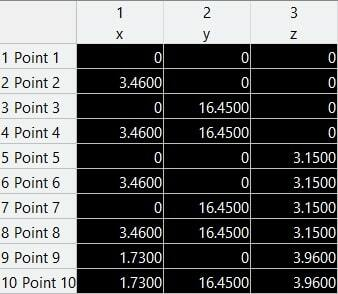
\includegraphics[scale=4.8]{Figures/matlab_grh_points_north.jpg}
        \caption*{(α)}{}
    \end{subfigure}%
    \begin{subfigure}{0.5\textwidth}
        \centering
        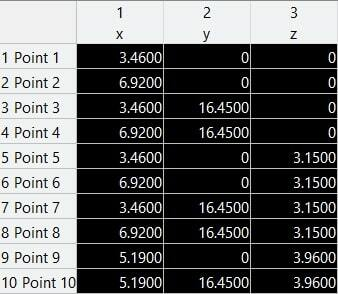
\includegraphics[scale=4.8]{Figures/matlab_grh_points_south.jpg}
        \caption*{(β)}{}
    \end{subfigure}%
    \caption{Σημεία (κορυφές) για (α) τη νότια και (β) τη βόρεια κατασκευαστική μονάδα του θερμοκηπίου.}
    \label{fig_matlab_points}
\end{figure}

Ο πλήρης αλγόριθμος εκτελέστηκε για τις προαναφερθείσες τρεις ημέρες και για τις 12:00:00. Οι Εικόνες 
\ref{fig_3D_dec}, \ref{fig_3D_mar} και \ref{fig_3D_jun} παρουσιάζουν τα τρισδιάστατα γραφικά που αποτελούνται 
από τις δύο κατασκευαστικές μονάδες, τα φωτοβολταϊκά, και τη σχηματιζόμενη από αυτά σκιά. Οι διαστάσεις είναι 
πραγματικές και εκφράζονται σε μέτρα, ενώ όπως και στην Εικόνα \ref{fig_sun_pos} για τη θέση του Ήλιου, οι άξονες 
\english{x} και \english{y} δείχνουν τον προσανατολισμό. Το ύψος του θερμοκηπίου από το έδαφος φαίνεται στον 
άξονα \english{z} των Εικόνων.

\clearpage

\begin{figure}[H]%
    \centering
    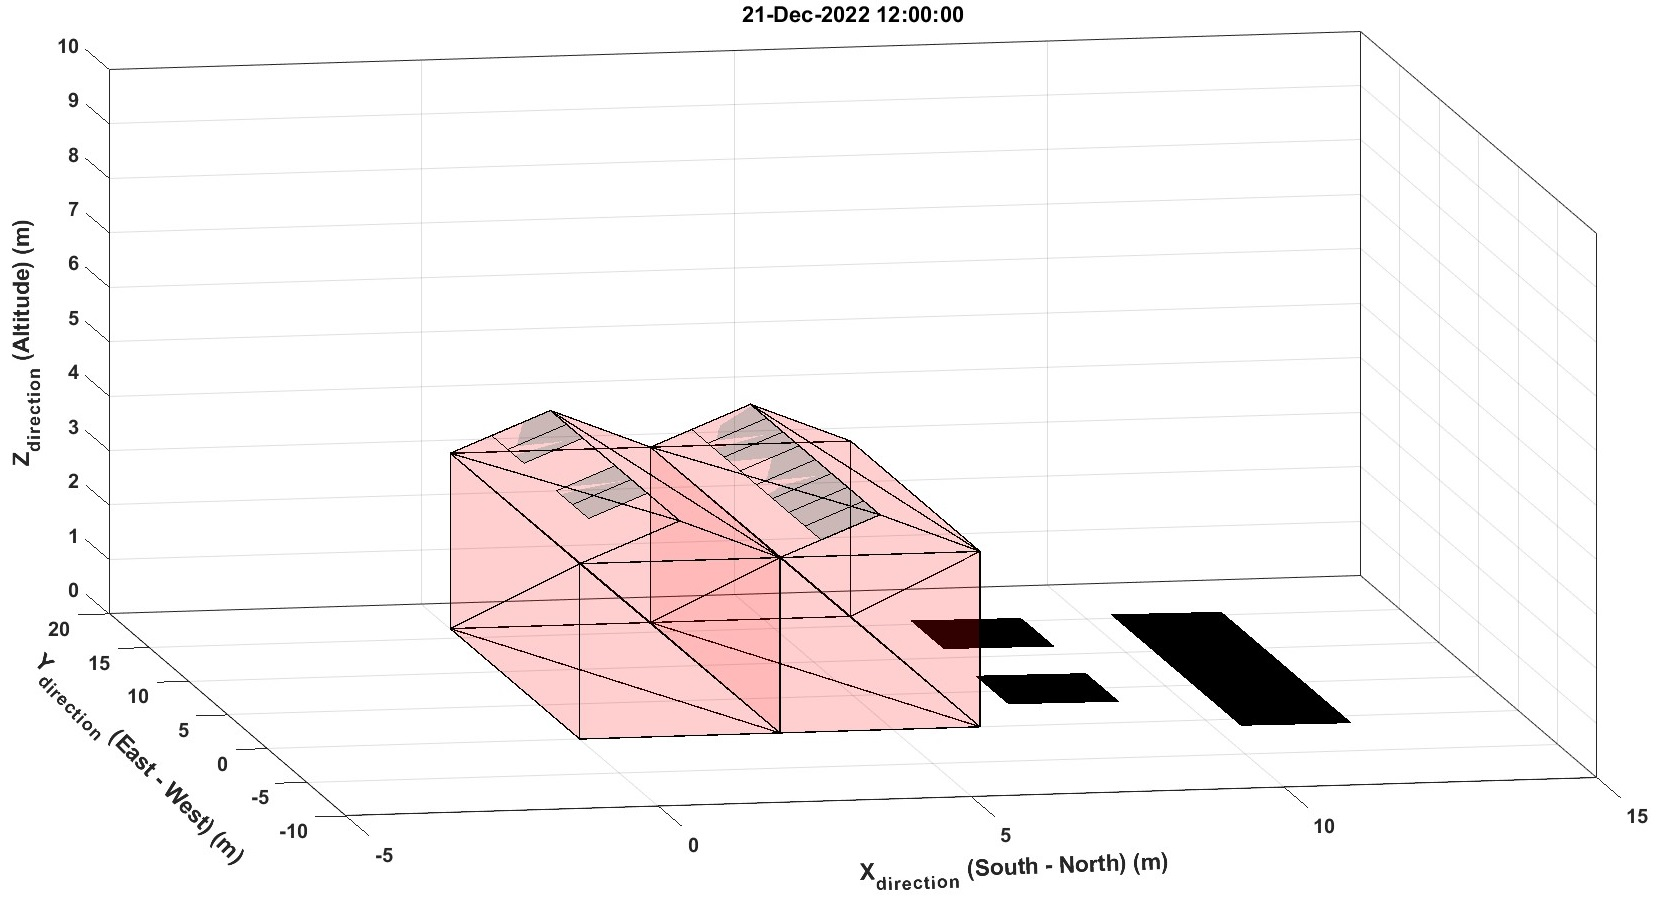
\includegraphics[width=0.9\textwidth]{Figures/3D_dec.jpg}
    \caption{\english{3D} αναπαράσταση του αποτελέσματος του αλγορίθμου για την 21η Δεκεμβρίου στις 12:00:00.}
    \label{fig_3D_dec}
\end{figure}

\begin{figure}[H]%
    \centering
    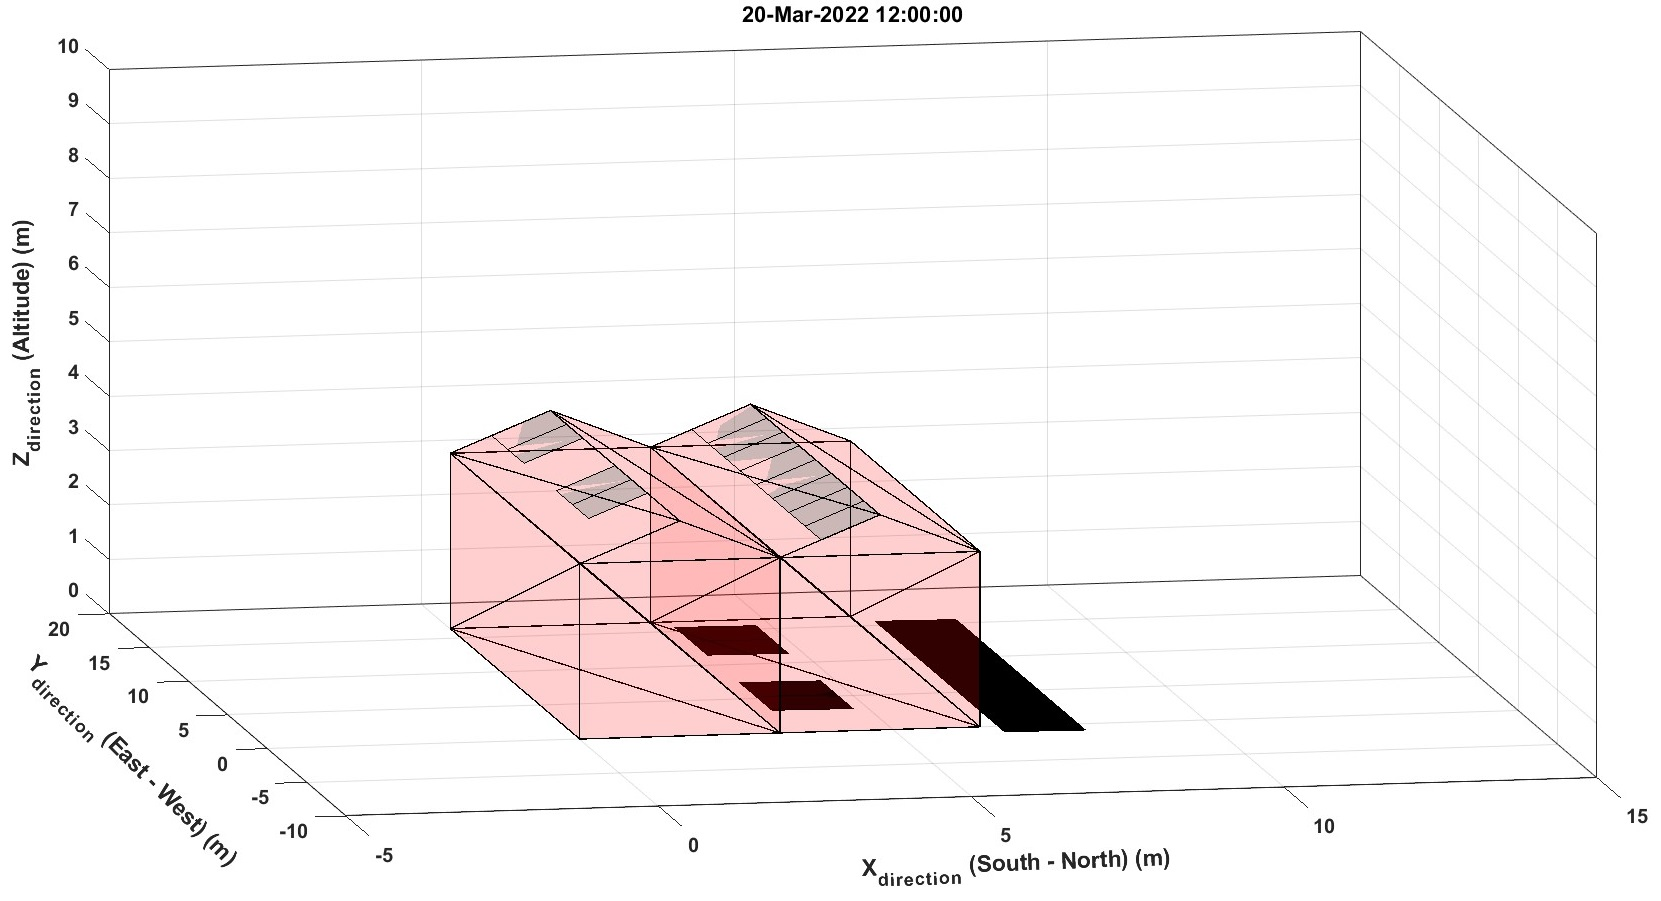
\includegraphics[width=0.9\textwidth]{Figures/3D_mar.jpg}
    \caption{\english{3D} αναπαράσταση του αποτελέσματος του αλγορίθμου για τις 20 Μαρτίου στις 12:00:00.}
    \label{fig_3D_mar}
\end{figure}

\clearpage

\begin{figure}[H]%
    \centering
    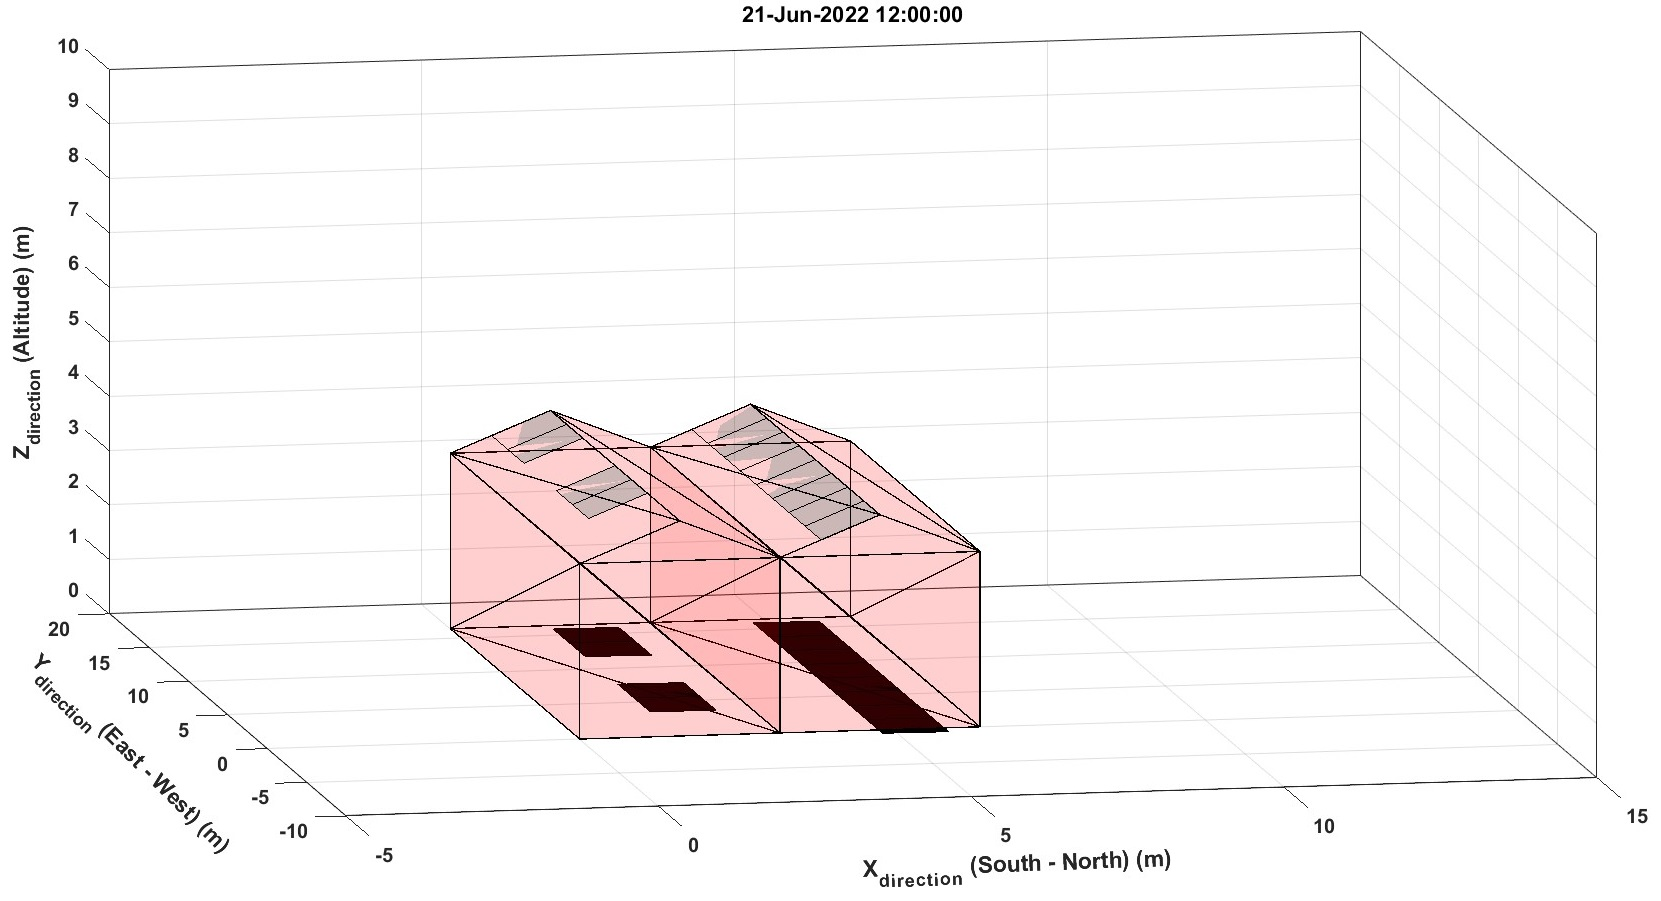
\includegraphics[width=0.9\textwidth]{Figures/3D_jun.jpg}
    \caption{\english{3D} αναπαράσταση του αποτελέσματος του αλγορίθμου για τις 21 Ιουνίου στις 12:00:00.}
    \label{fig_3D_jun}
\end{figure}

Η εκτέλεση του αλγόριθμου για την ίδια χρονική στιγμή της ημέρας και στα τρία σενάρια αποκαλύπτει την παράλληλη ως προς 
τον άξονα \english{x} τροχιά της σχηματισμένης σκιάς. Αντίθετα, κατά την περίοδο από τον Δεκέμβριο έως τον Ιούνιο, ο ήλιος 
προοδευτικά ανυψώνεται, οδηγώντας σε μια πιο απότομη γωνία πρόσπτωσης της ηλιακής ακτινοβολίας. Κατά συνέπεια, η σκιά 
μετατοπίζεται σταδιακά σε θέση ακριβώς κάτω από το φωτοβολταϊκό σύστημα και εντός των ορίων του θερμοκηπίου, ενώ η 
επιφάνειά της μειώνεται με την πάροδο του χρόνου.

Στις Εικόνες \ref{fig_2D_dec}, \ref{fig_2D_mar} και \ref{fig_2D_jun} παρουσιάζονται τα αποτελέσματα του αλγορίθμου όσον 
αφορά τις απεικονίσεις δύο διαστάσεων. Στις συγκεκριμένες περιπτώσεις παρουσιάζονται οι κατόψεις των παραπάνω καταστάσεων, 
με την παρουσία ή απουσία της σκιάς (ανοιχτό γκρι, έντονο γκρι και μαύρο για τις διάφορες φωτοβολταϊκές συστοιχίες) και την 
παρουσία των θερμοκηπιακών μονάδων κατασκευής (κόκκινο για τη νότια και μπλε για τη βόρεια κατασκευαστική μονάδα). Οι 
διαστάσεις στους άξονες περιγράφονται σε \SI{}{\centi\meter}, καθώς τα συγκεκριμένα γραφικά αποτελούν μια πιο άμεση 
αναπαράσταση των ποσοτικών αποτελεσμάτων (περιοχή σκιάς) πριν από τη μετατροπή τους σε \SI{}{\meter\squared} στο Τμήμα 3 
του αλγορίθμου. Ταυτόχρονα, οι σκιές έξω από το θερμοκήπιο λείπουν στις συγκεκριμένες περιπτώσεις, καθώς λαμβάνονται υπόψη 
μόνο εκείνες που βρίσκονται μέσα στο θερμοκήπιο. Τέλος, στον Πίνακα 7 παρουσιάζεται το εμβαδόν της σκιάς (\SI{}{\meter\squared}) 
που βρίσκεται εντός της βόρειας κατασκευαστικής μονάδας και το ποσοστό της επί της συνολικής επιφάνειας της μονάδας.

\begin{figure}[h]%
    \centering
    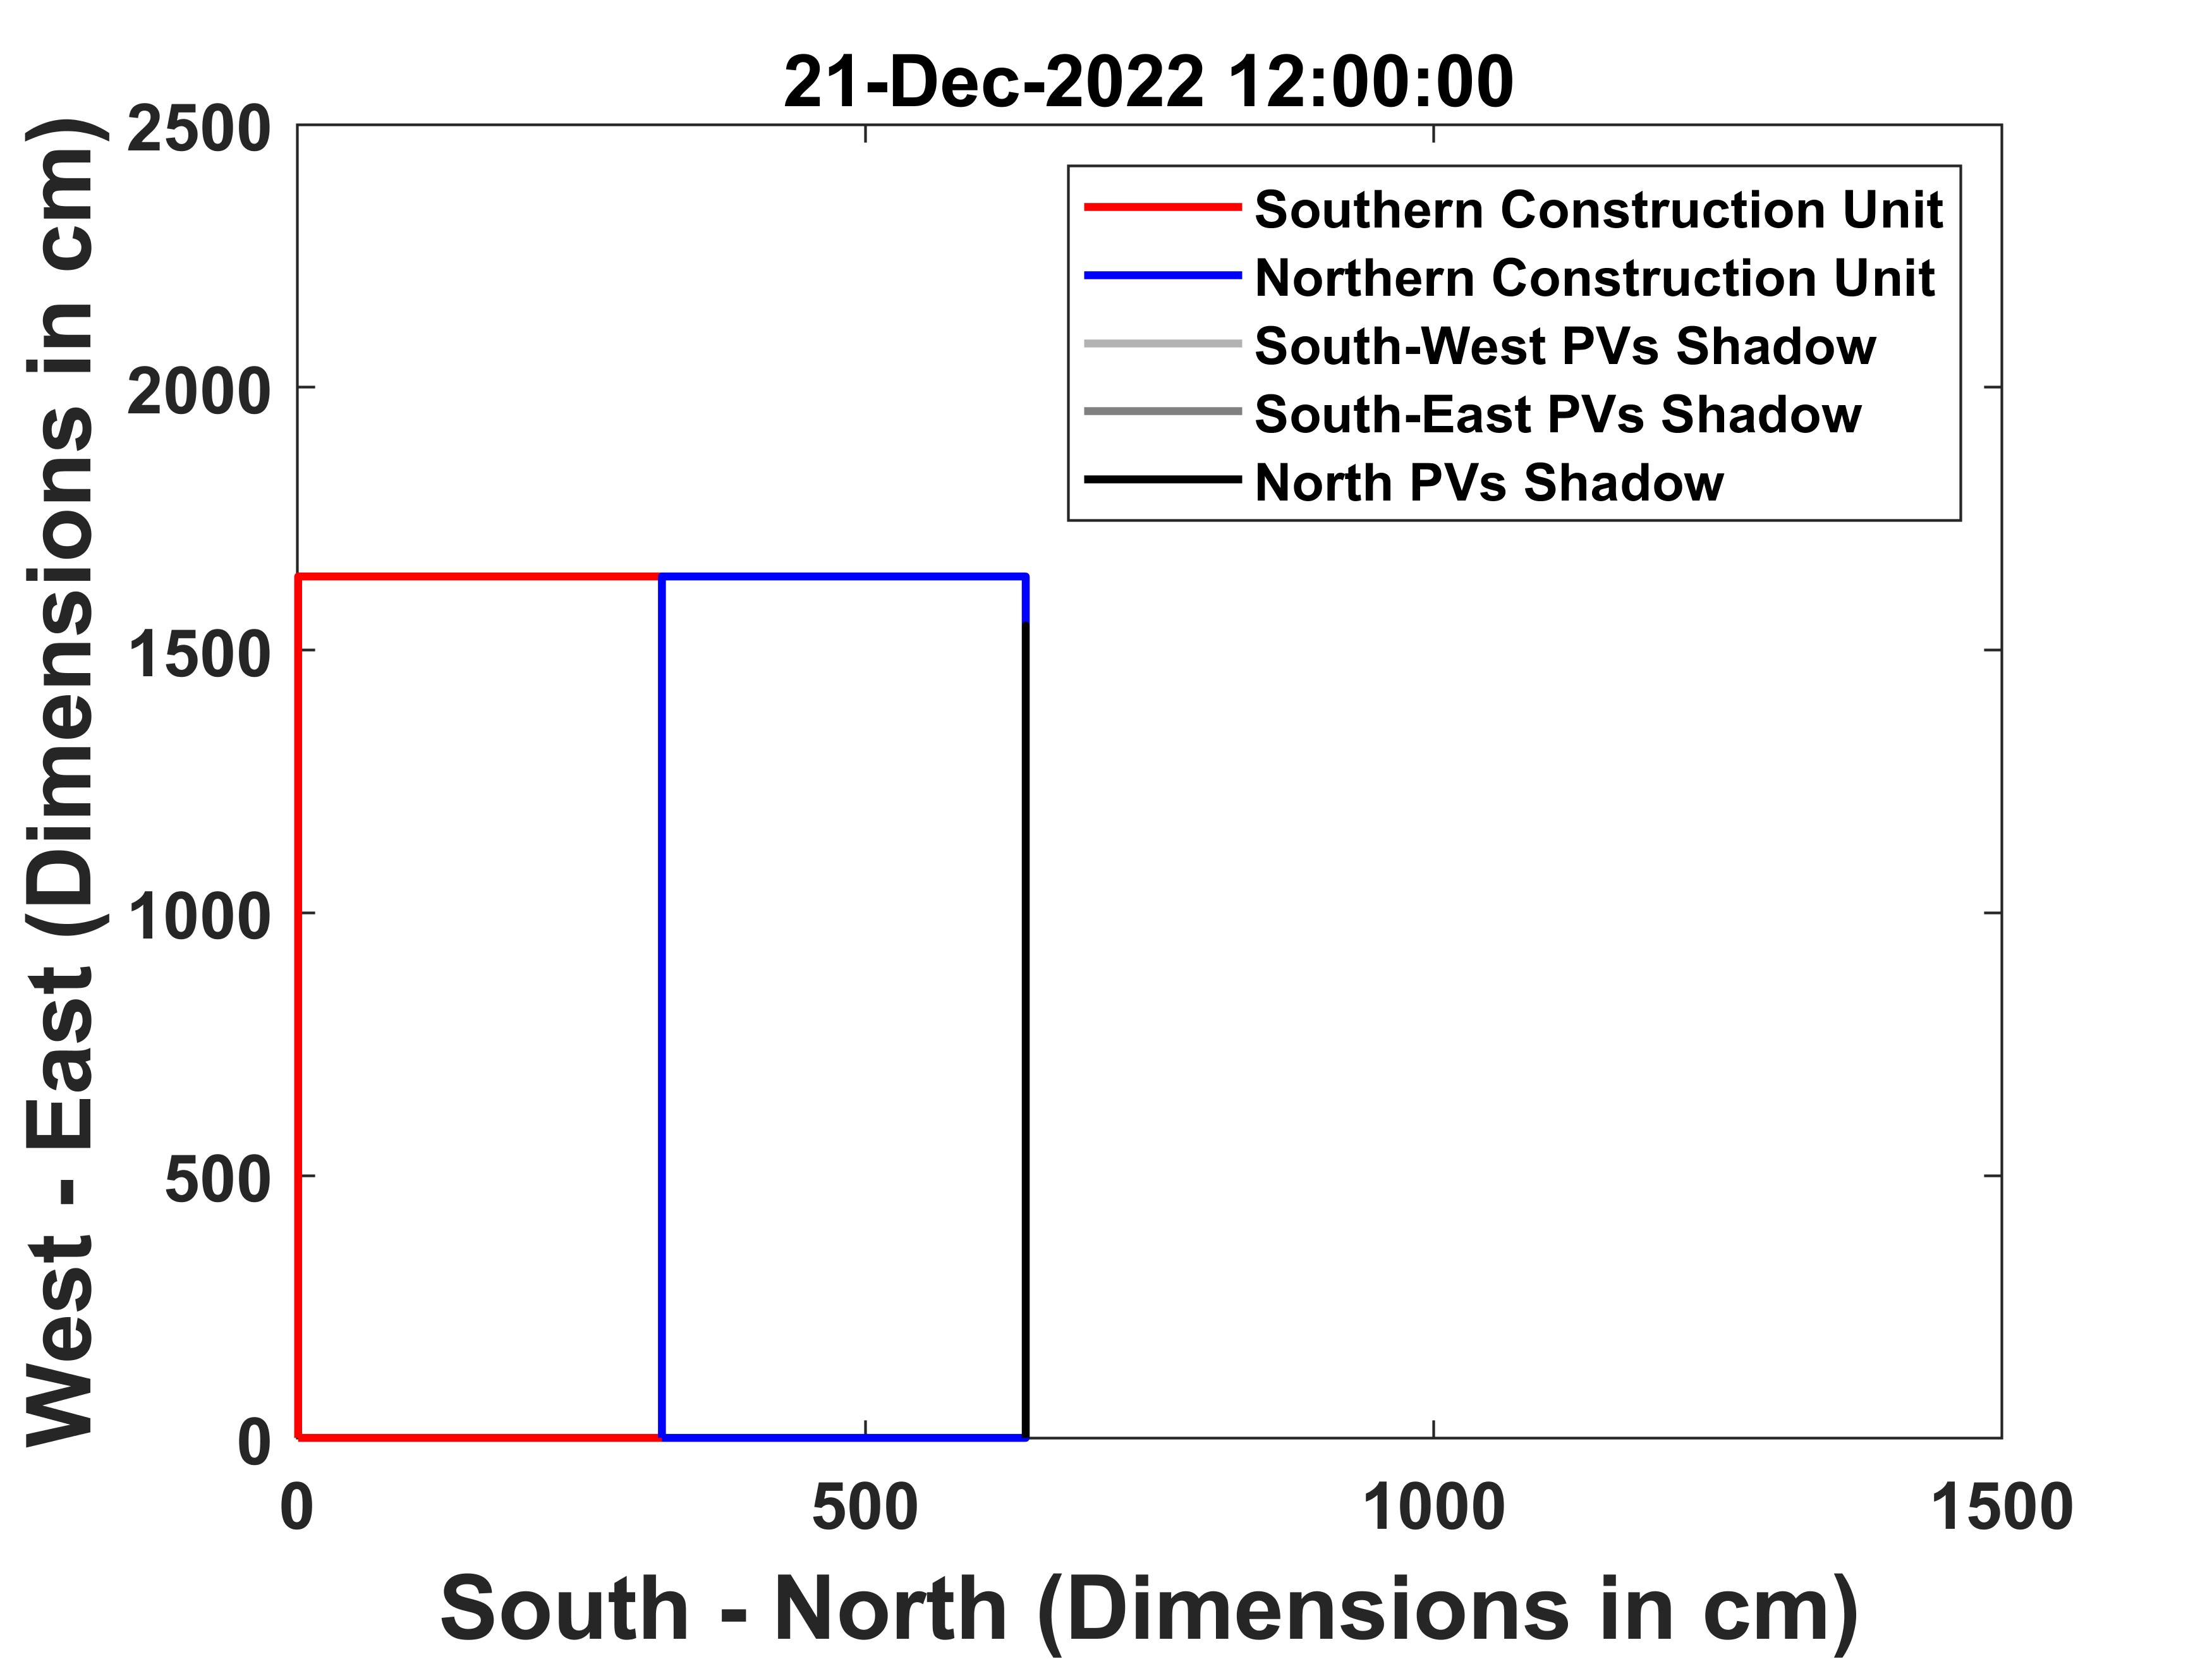
\includegraphics[scale = 0.073]{Figures/2D_dec.jpg}
    \caption{\english{2D} αναπαράσταση του αποτελέσματος του αλγορίθμου για την 21η Δεκεμβρίου στις 12:00:00.}
    \label{fig_2D_dec}
\end{figure}

\begin{figure}[h]%
    \centering
    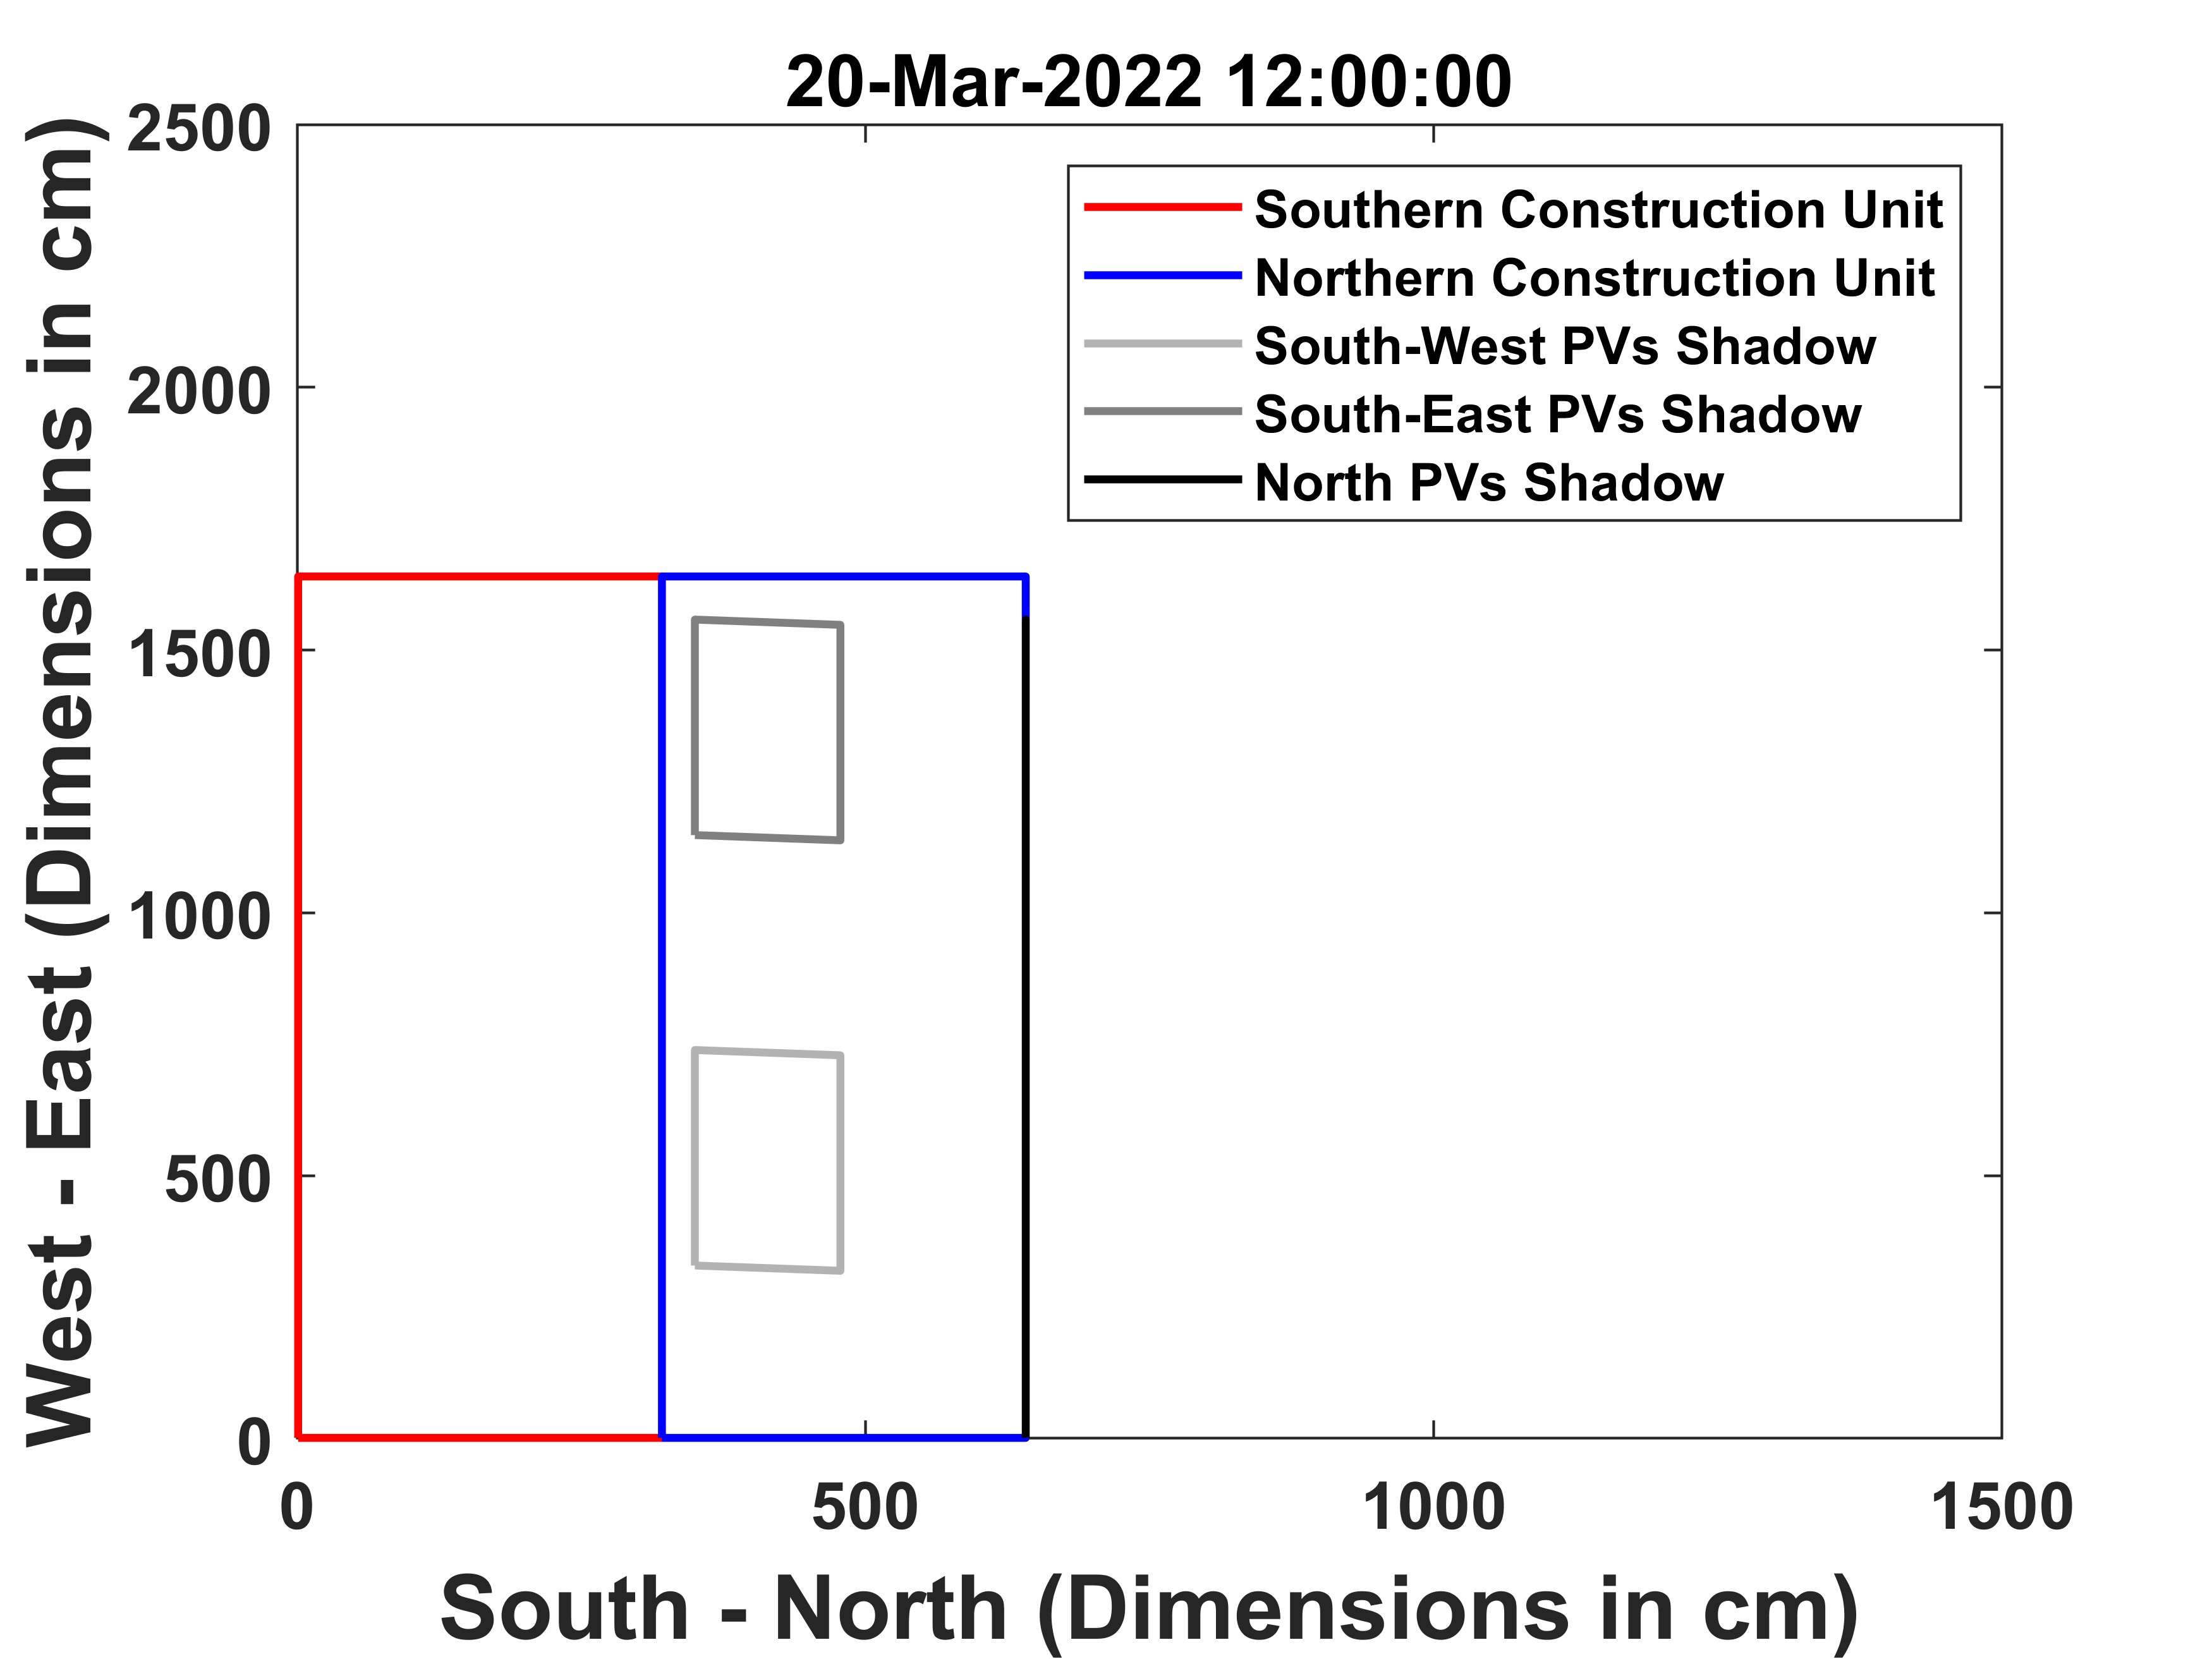
\includegraphics[scale = 0.073]{Figures/2D_mar.jpg}
    \caption{\english{2D} αναπαράσταση του αποτελέσματος του αλγορίθμου για τις 20 Μαρτίου στις 12:00:00.}
    \label{fig_2D_mar}
\end{figure}

\begin{figure}[h]%
    \centering
    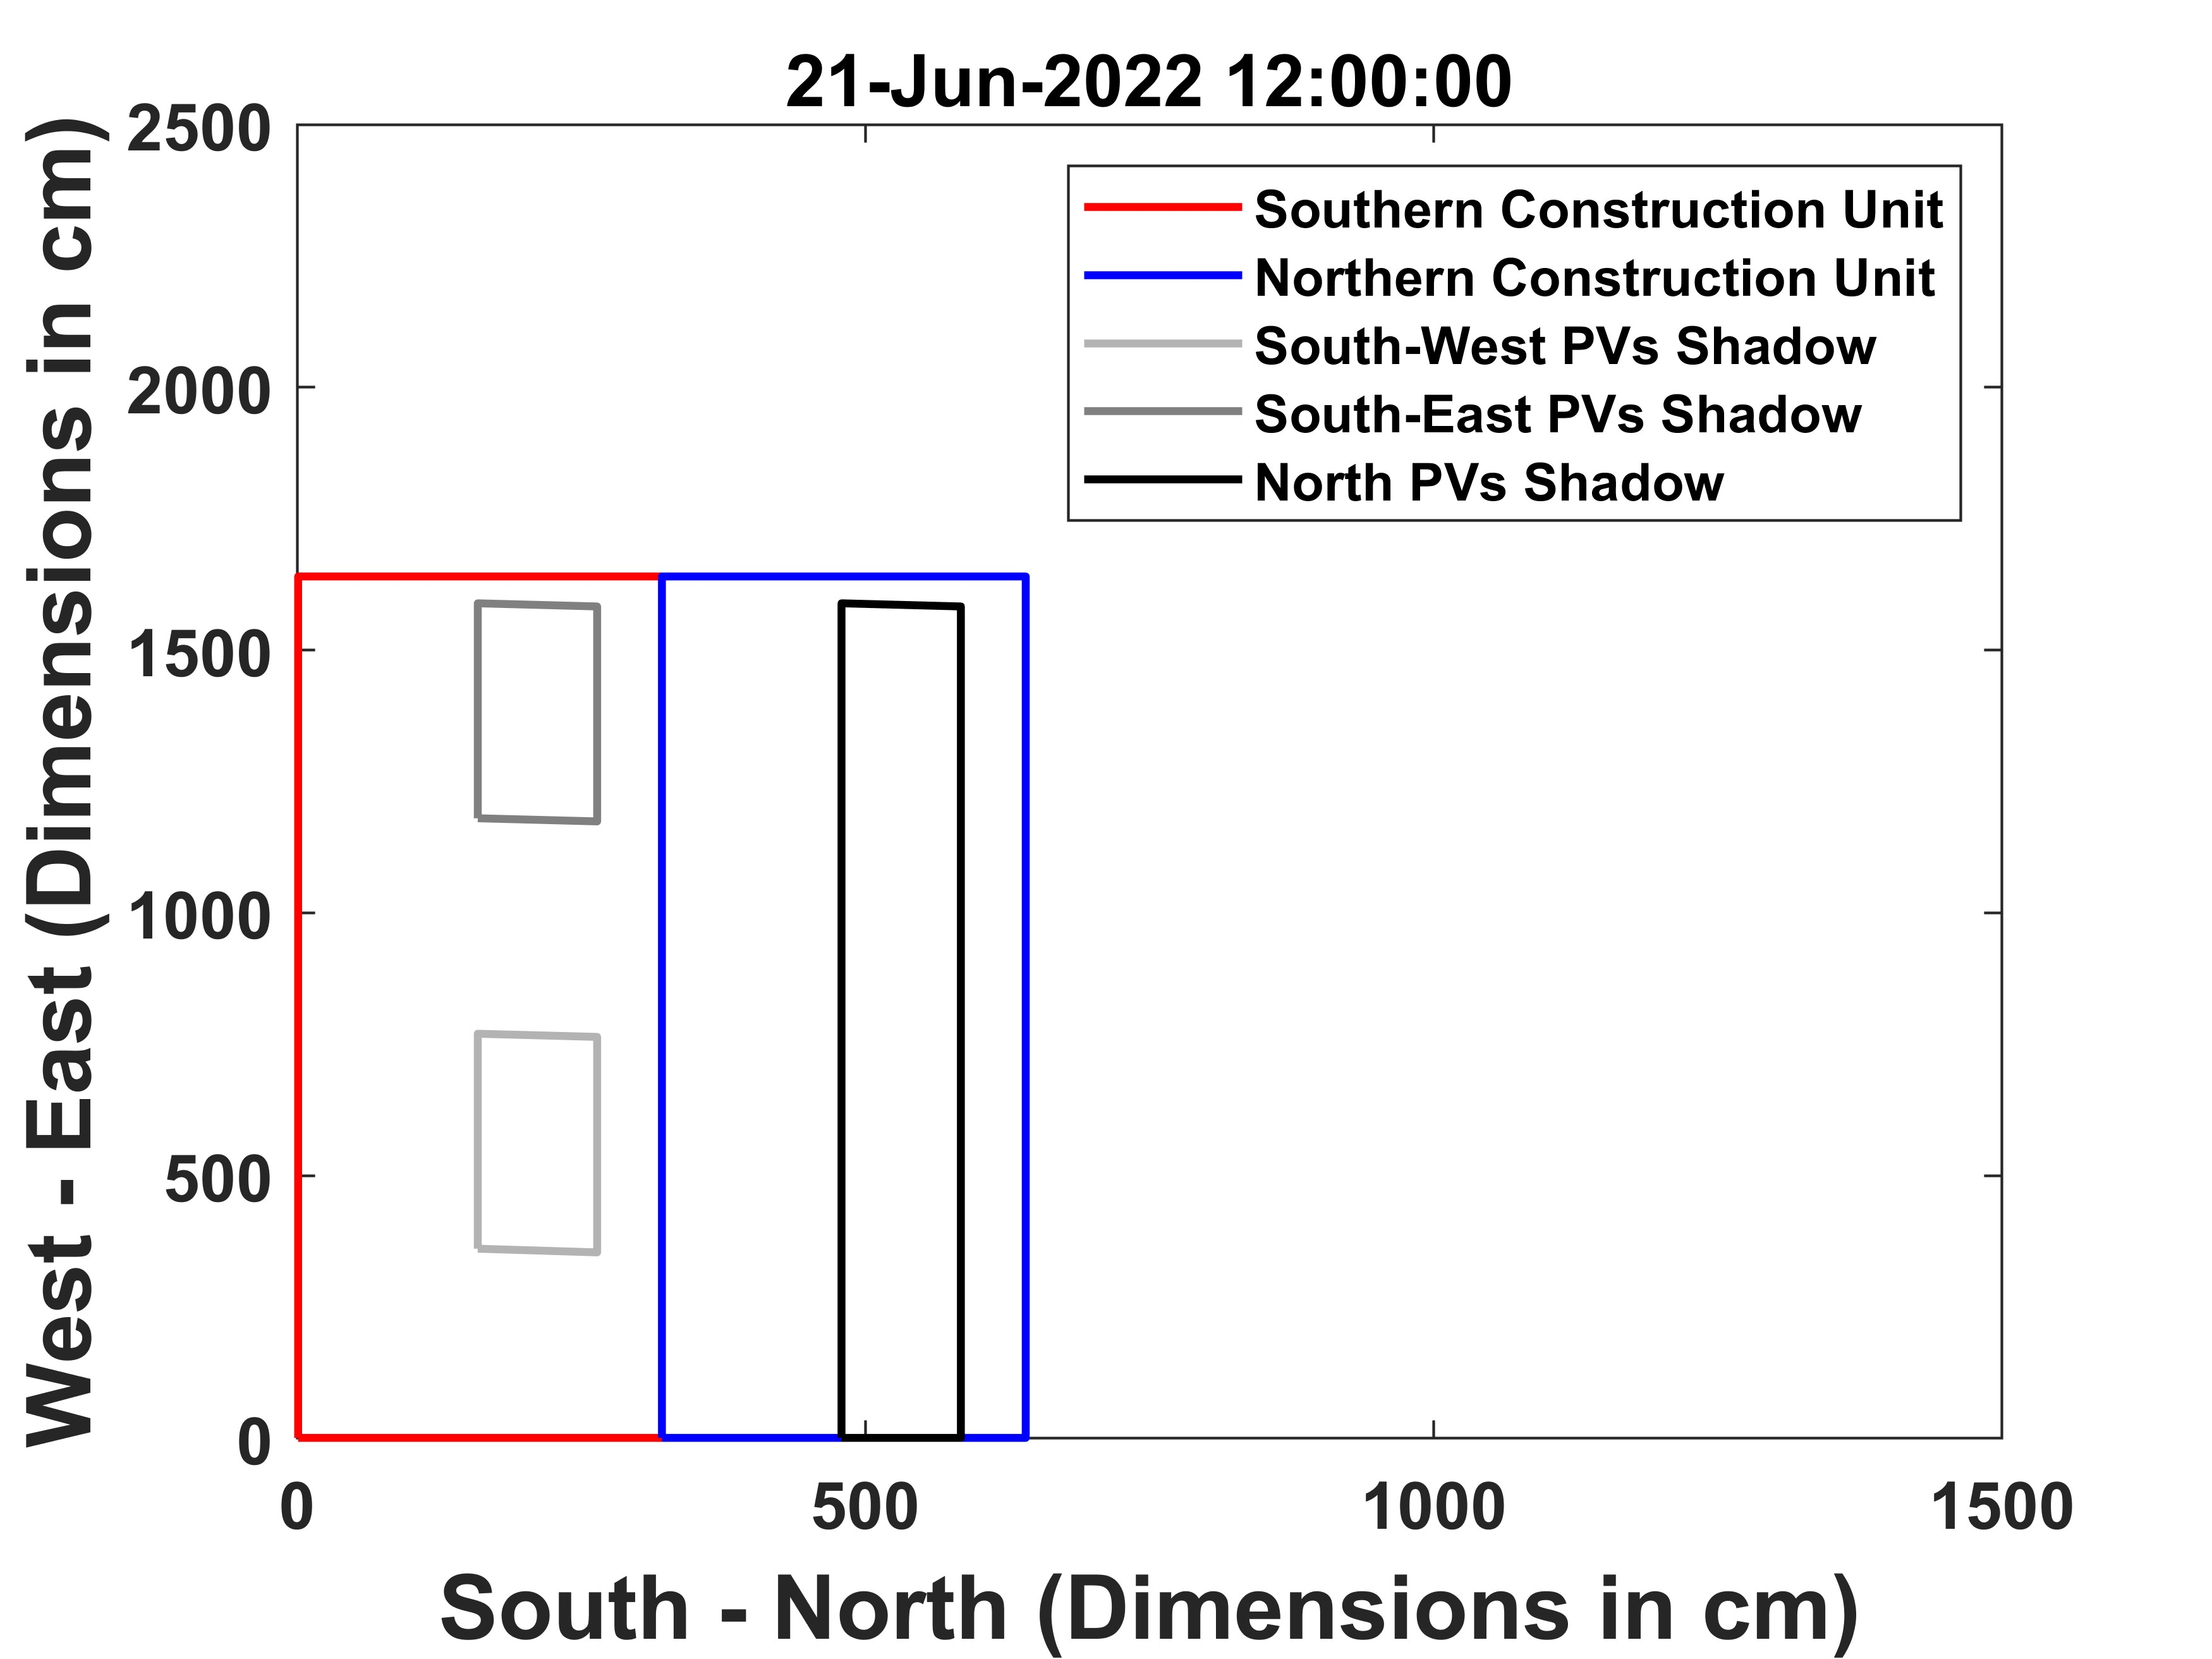
\includegraphics[scale = 0.073]{Figures/2D_jun.jpg}
    \caption{\english{2D} αναπαράσταση του αποτελέσματος του αλγορίθμου για τις 21 Ιουνίου στις 12:00:00.}
    \label{fig_2D_jun}
\end{figure}

\clearpage

\begin{table}[ht]
    \centering
    \caption{Σκιασμένη επιφάνεια εντός της βόρειας κατασκευαστικής μονάδας του θερμοκηπίου και ποσοστό κάλυψης για τις 21 Δεκεμβρίου, 20 Μαρτίου και 21 Ιουνίου.}\label{tab_alg_results} 
   \begin{tabular}{>{\centering\arraybackslash}m{4.85cm} >{\centering\arraybackslash}m{4.85cm} >{\centering\arraybackslash}m{4.85cm}}
        \toprule
        \textbf{Ημέρα στις 12:00:00} & \textbf{Σκιασμένη επιφάνεια (\SI{}{\meter\squared})} & \textbf{Ποσοστιαία κάλυψη (\SI{}{\percent})} \\
        \midrule
        21 Δεκεμβρίου & 0 & 0 \\
        20 Μαρτίου & 10,5 & 20,01 \\
        21 Ιουνίου & 16,64 & 31,73 \\   
        \bottomrule
    \end{tabular}
\end{table}

Στην Εικόνα \ref{fig_diurnal_perc} παρουσιάζεται το ποσοστό της επί της συνολικής επιφάνειας της μονάδας για τις τρεις 
διαφορετικές περιπτώσεις των τριών ημερων. Εκτός από την ημέρα για τις 21 Δεκεμβρίου, όπου το εσωτερικό της βόρειας 
κατασκευαστικής μονάδας δεν είναι καθόλου σκιασμένο, οι άλλες δύο περιπτώσεις παρουσιάζουν κάλυψη από την σχηματιζόμενη 
σκιά, με ένα μέγιστο περίπου κατά το μεσημέρι, όταν ο Ήλιος βρίσκεται σε θέση πάνω από το θερμοκήπιο, με ποσοστό 
\SI{19,94}{\percent} για τις 20 Μαρτίου στις 12:40:00 και \SI{33,19}{\percent} για τις 21 Ιουνίου στις 12:30:00. Παρουσιάζεται 
επίσης διαφορά στο μοτίβο της καμπύλης μεταξύ των δύο ημερών, με την καμπύλη της 21ης Ιουνίου να εμφανίζεται πιο συμμετρική 
ως προς το χρονικό σημείο του μέγιστου, σε σύγκριση με εκείνη της 20ης Μαρτίου. Αυτό οφείλεται στο γεγονός ότι για την 
περίπτωση της 21ης Ιουνίου, η σκίαση σχηματίζεται από τα φωτοβολταϊκά που βρίσκονται στη στέγη της βόρειας μονάδας και 
καλύπτουν το σύνολό της ως προς την κατεύθυνση του άξονα \english{y} (Εικόνες \ref{fig_3D_jun} και \ref{fig_2D_jun}), με 
αποτέλεσμα την απόλυτη συμμετρία γύρω από το κέντρο του θερμοκηπίου. Αντίθετα, η σκιά για την περίπτωση της 20ης Μαρτίου 
οφείλεται στα φωτοβολταϊκά που βρίσκονται στην παρακείμενη μονάδα (Εικόνες \ref{fig_3D_mar} και \ref{fig_2D_mar}), και σε 
αντίθεση με την πρώτη περίπτωση, παρουσιάζουν ασυνέχεια και ασυμμετρία ως προς την τοποθέτησή τους.

\begin{figure}[ht]%
    \centering
    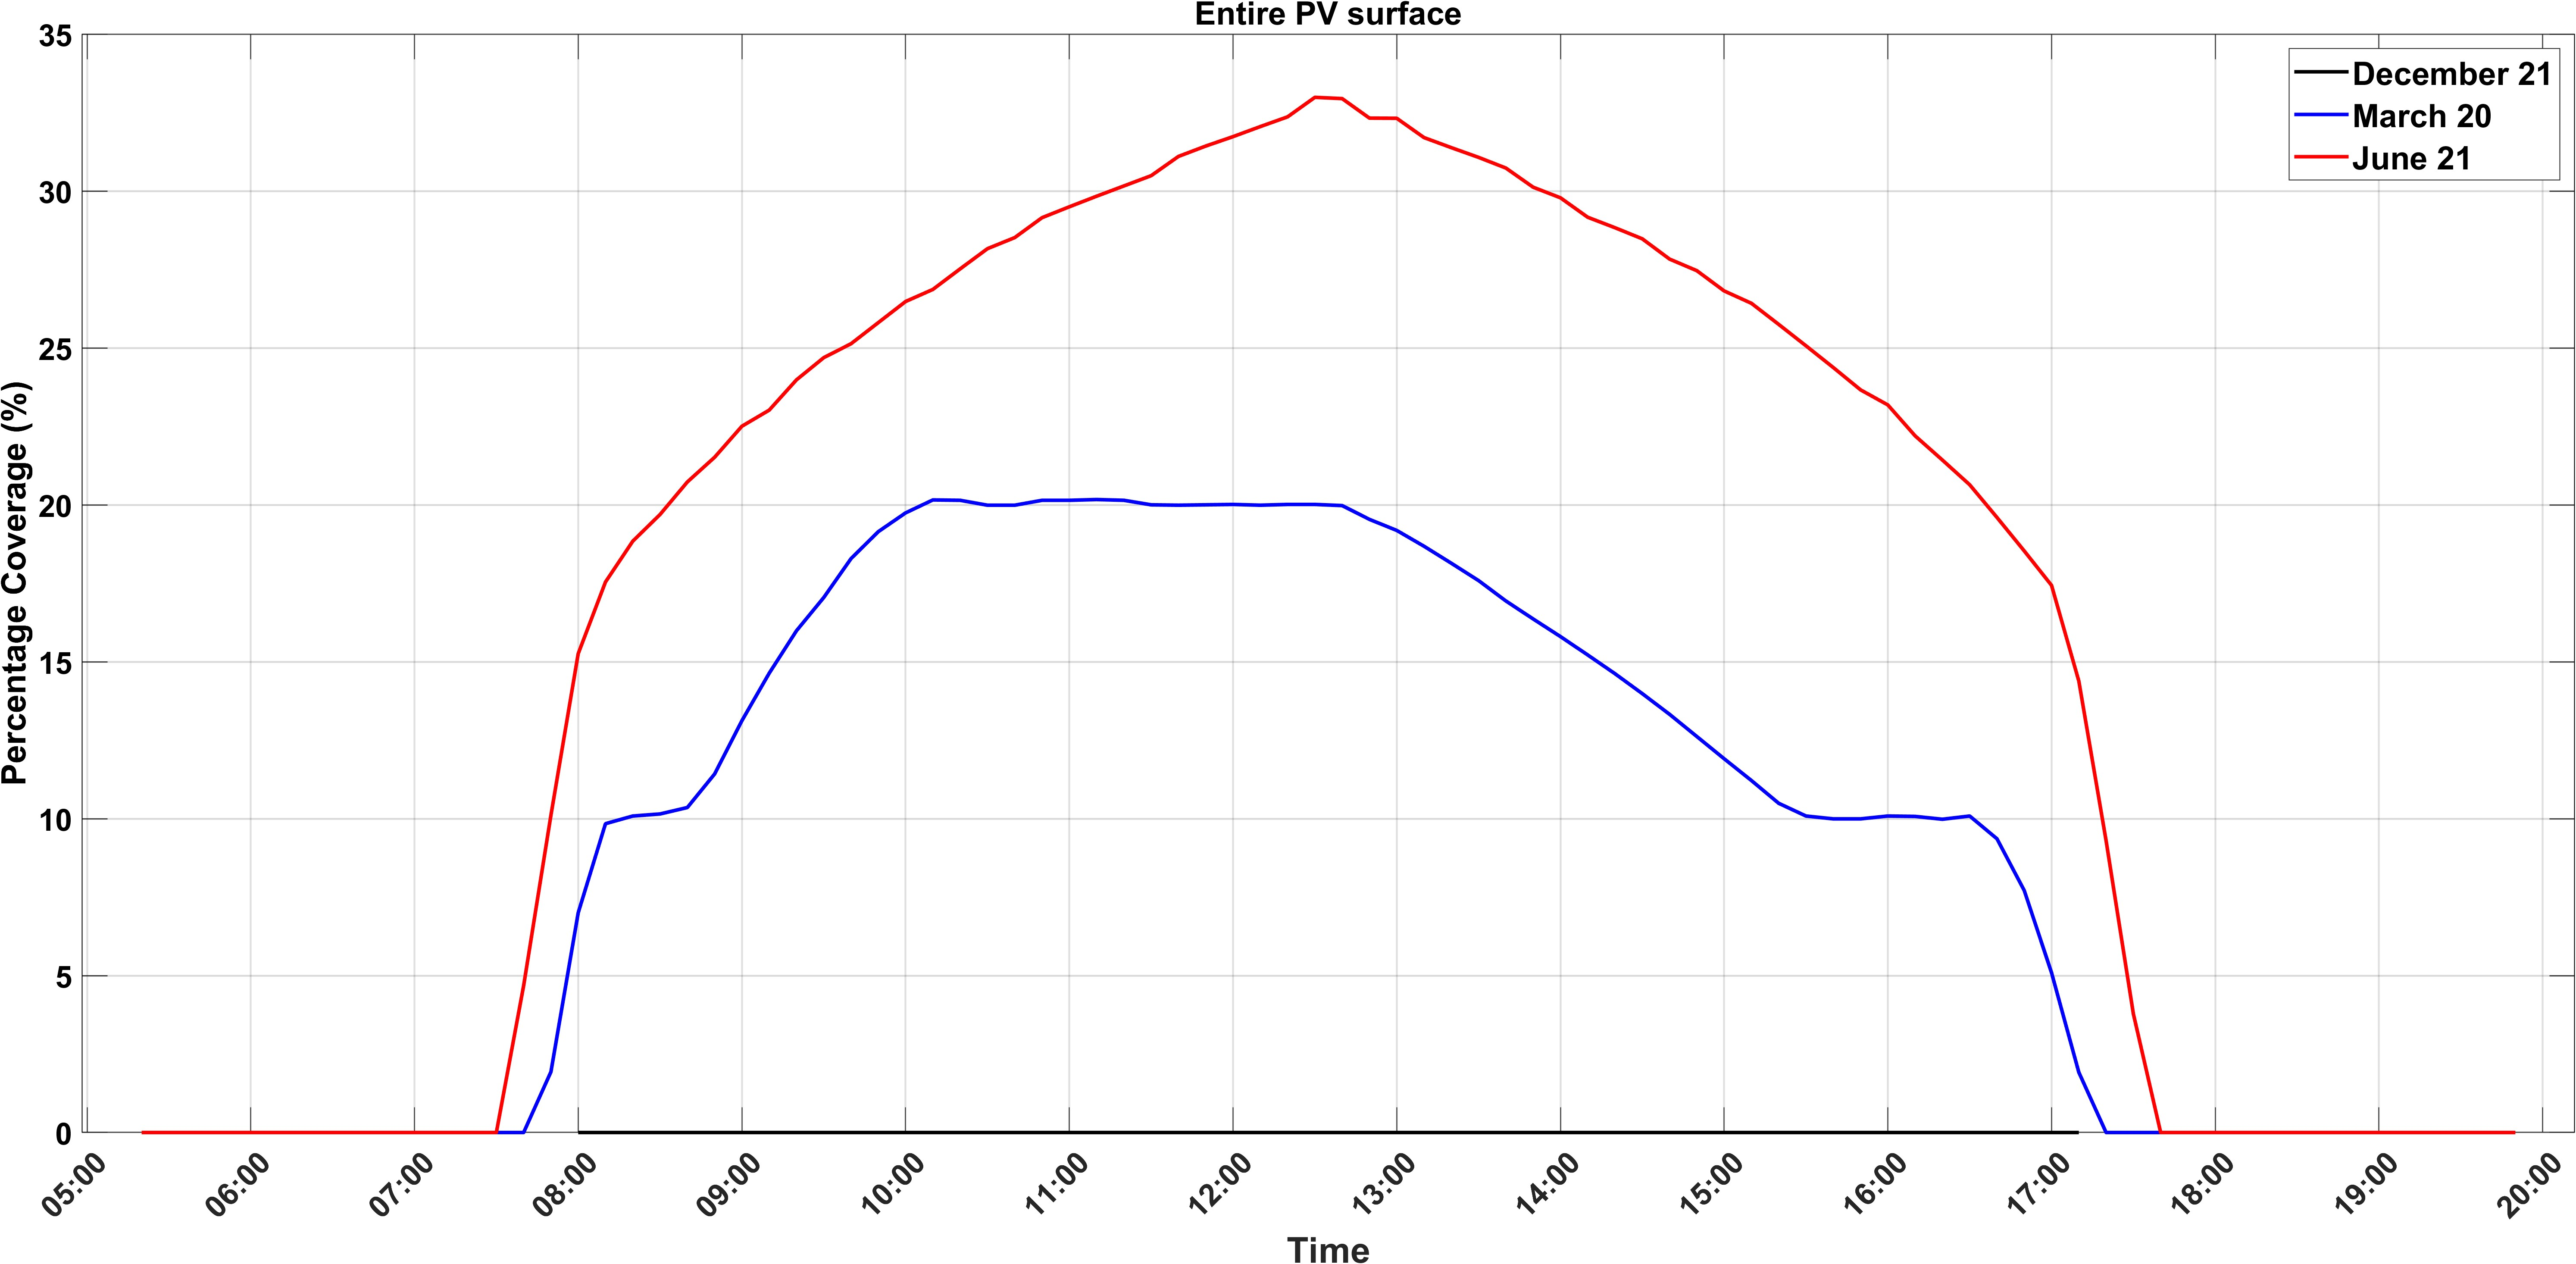
\includegraphics[width=0.9\textwidth]{Figures/diurnal_perc.jpg}
    \caption{Ημερήσιο ποσοστό κάλυψης σκίασης για τις 21 Δεκεμβρίου, 20 Μαρτίου και 21 Ιουνίου.}
    \label{fig_diurnal_perc}
\end{figure}

Τέλος, στην Εικόνα \ref{fig_annual_perc} παρουσιάζονται τα αποτελέσματα του αλγορίθμου καθ' όλη τη διάρκεια του έτους 2022 
με χρονικό βήμα 10 λεπτών. Η γραφική παράσταση της Εικόνας 14 αποτελείται από 52.560 τιμές (365 ημέρες $\cdot$ 24 ώρες 
$\cdot$ 6 περίοδοι των 10 λεπτών), εκ των οποίων τα χρονικά διαστήματα λίγο πριν την ανατολή και αμέσως μετά τη δύση του 
ηλίου λαμβάνουν τιμές “\english{NaN}”. Οι ημερήσιες διακυμάνσεις της σκίασης δεν είναι αντιληπτές σε αυτή την περίπτωση, 
αλλά αντίθετα διαμορφώνεται ένα μεγαλύτερο μοτίβο σκίασης από τα φωτοβολταϊκά. Συγκεκριμένα, παρατηρούνται δύο τοπικά 
μέγιστα, δύο ολικά μέγιστα και τρία τοπικά ελάχιστα. Το πρώτο και δεύτερο τοπικό μέγιστο στις 17 Φεβρουαρίου και 26 
Οκτωβρίου με ποσοστό κάλυψης ίσο με \SI{22,84}{\percent} και \SI{22,81}{\percent}, αντίστοιχα, σχετίζονται με τη σκίαση 
που προκαλείται από τα φωτοβολταϊκά που είναι εγκατεστημένα στη νότια κατασκευαστική μονάδα του θερμοκηπίου. Οι μειωμένες 
τιμές, κατά περίπου \SI{53}{\percent} από τα ολικά μέγιστα που παρουσιάζονται στις 5 Μαΐου και 9 Αυγούστου, οφείλονται στην 
ασυνέχεια των φωτοβολταϊκών συστοιχιών και την ελλιπή κάλυψη της στέγης της νότιας μονάδας. Από την άλλη, τα δύο ολικά 
μέγιστα των παραπάνω ημερομηνιών με τιμές ίσες με περίπου \SI{35}{\percent}, οφείλονται στην πλήρη κάλυψη του νότιου κεκλιμένου 
επιπέδου της οροφής της βόρειας κατασκευαστικής μονάδας. Έτσι, δεδομένου ότι οι τιμές που λαμβάνονται υπόψη σε αυτή την 
Εικόνα είναι οι ημερήσιες μέγιστες τιμές, είναι αποδεκτό το γεγονός της μείωσης τον μήνα Φεβρουάριο κατά περίπου 
\SI{50}{\percent} σε σχέση με τον Μάιο, καθώς τον Φεβρουάριο, τα φωτοβολταϊκά που συμμετέχουν στη σκίαση του θερμοκηπίου είναι 
τέσσερα, σε αντίθεση με τον Μάιο που η σκίαση προκαλείται από τα οκτώ φωτοβολταϊκά της βορινής βασικής κατασκευαστικής μονάδας.

\begin{figure}[ht]%
    \centering
    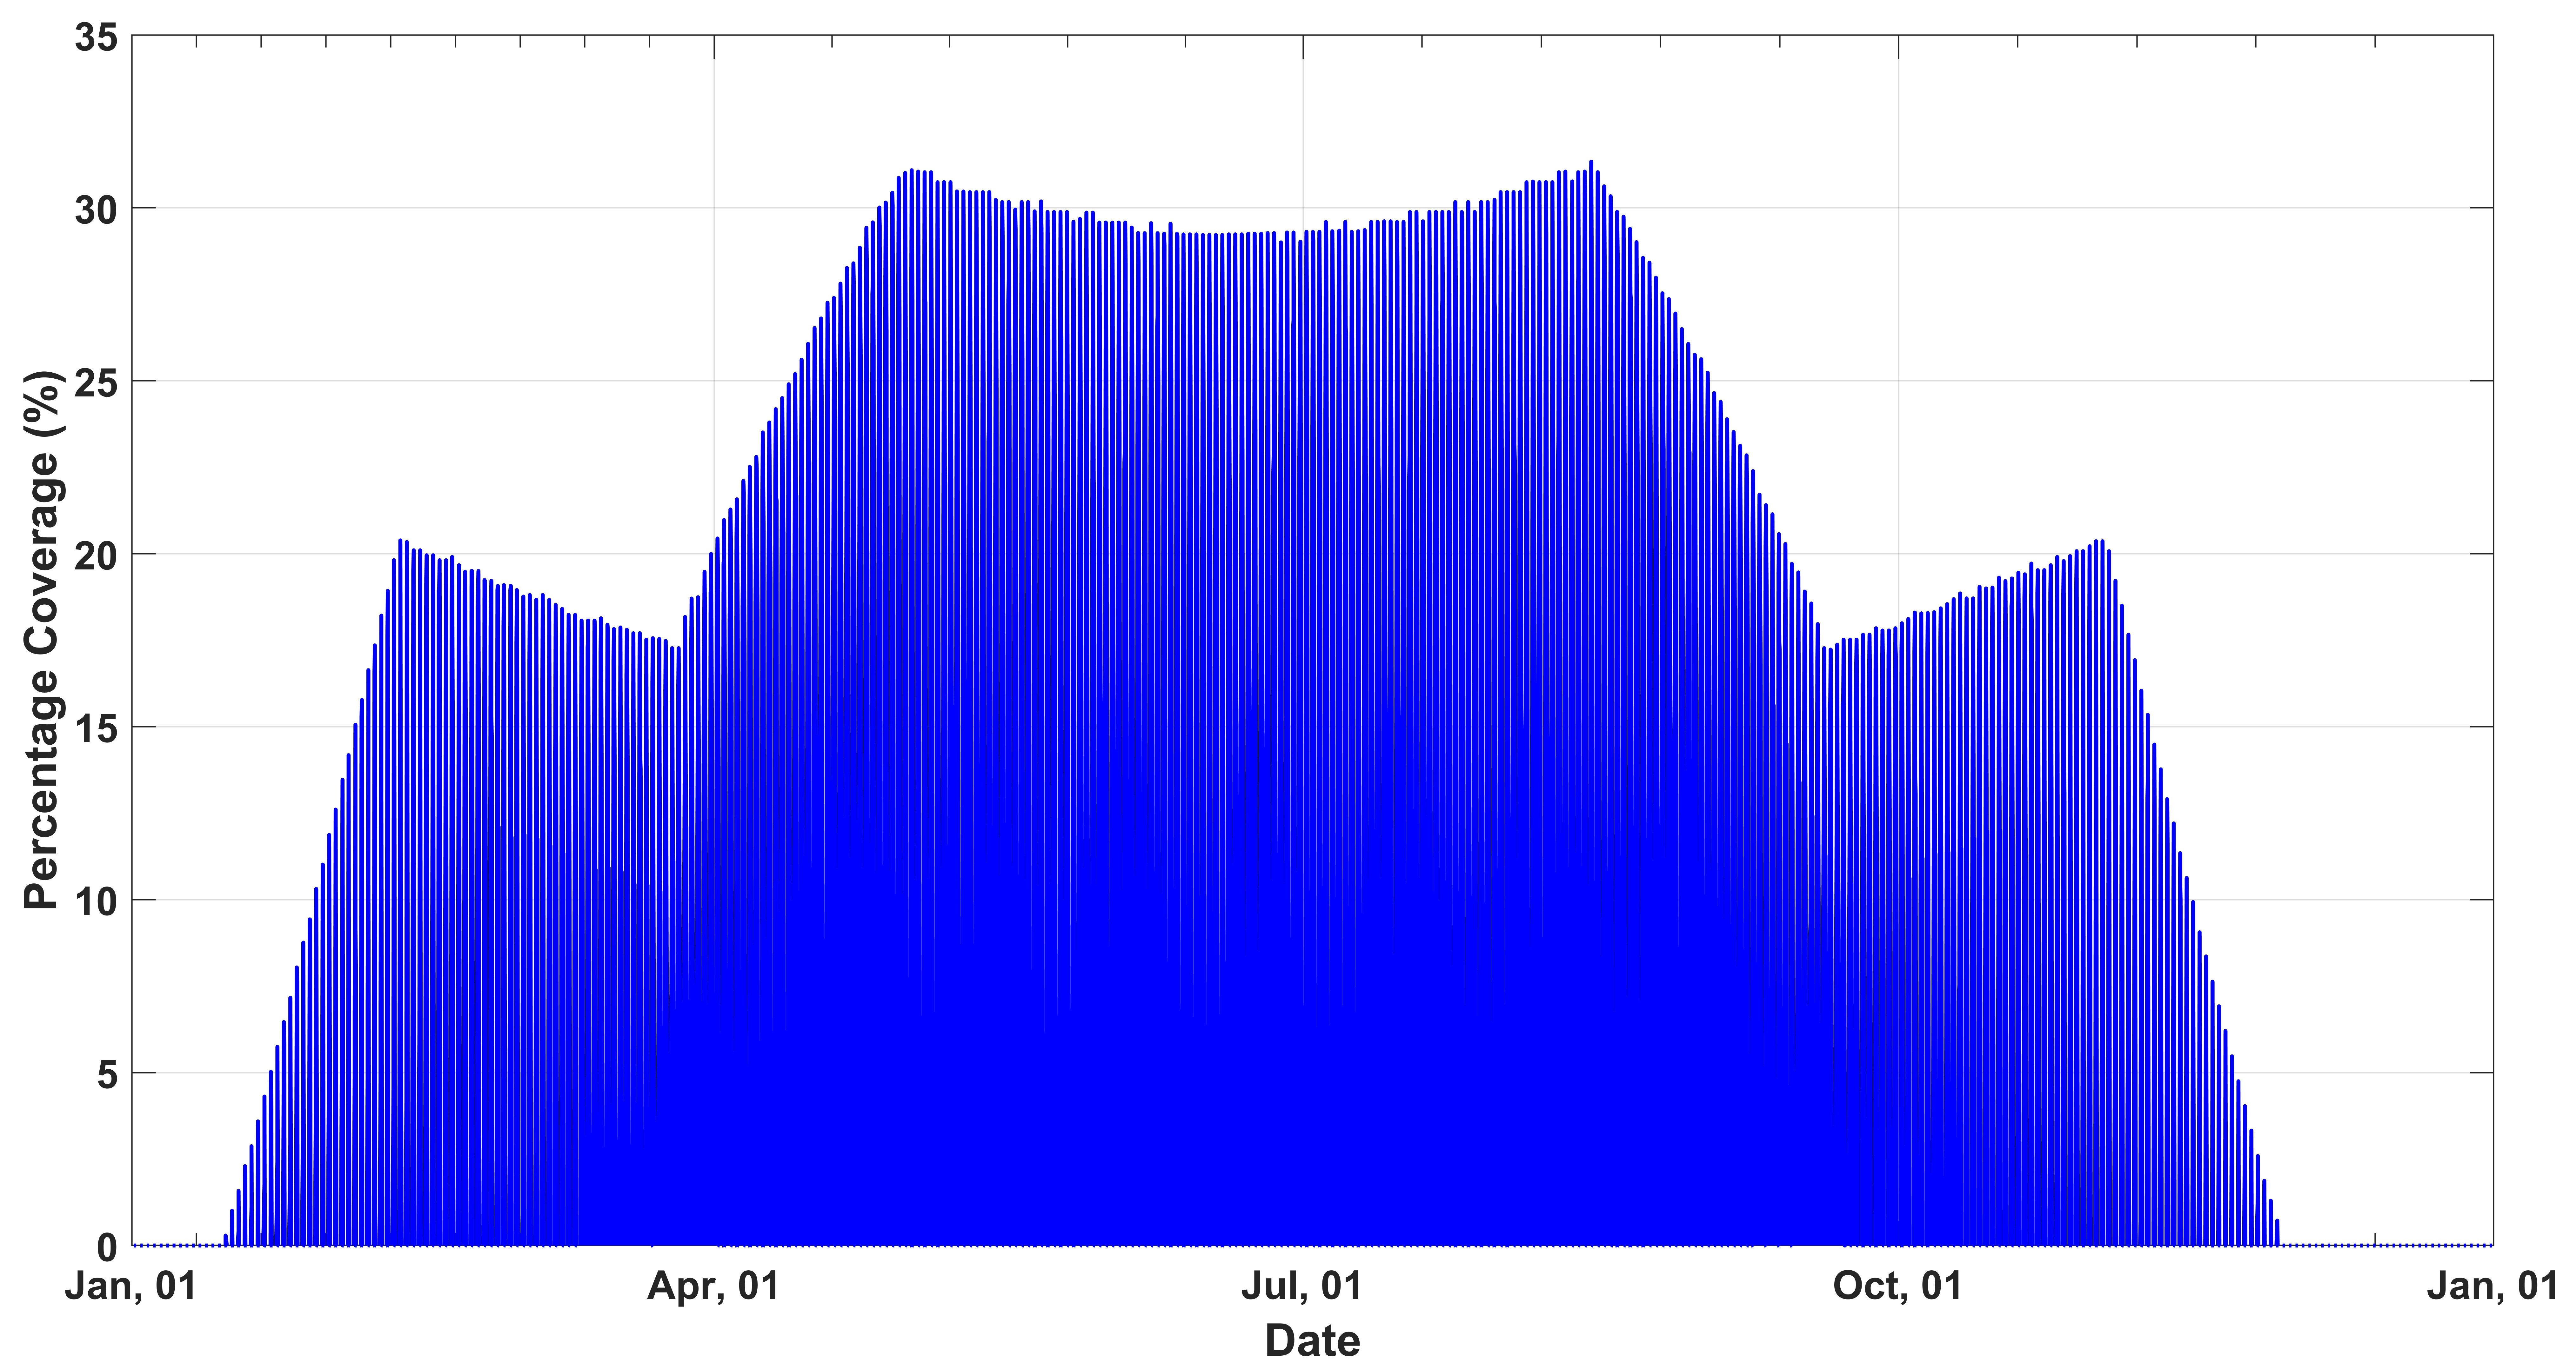
\includegraphics[width=0.9\textwidth]{Figures/annual_perc.jpg}
    \caption{Ετήσιο ποσοστό κάλυψης σκίασης.}
    \label{fig_annual_perc}
\end{figure}

\subsubsection{Αποτελέσματα επικύρωσης του αλγορίθμου}\label{subsub_alg_valid}

Όπως περιγράφεται στην Παράγραφο \ref{subsub_validation}, για την επικύρωση του μοντέλου, τα ενσωματωμένα στην οροφή 
του θερμοκηπίου φωτοβολταϊκά καλύφθηκαν με ένα αδιαφανές μέσο, προκειμένου να δημιουργηθεί μια ισχυρή σκίαση κάτω από 
αυτά. Η έντονη αυτή σκίαση δεν θα ήταν δυνατόν να διαμορφωθεί από τα υπάρχοντα ημιδιαφανή φωτοβολταϊκά, κάθως η σκίαση 
που προσφέρει κάθε μία από αυτές τις μονάδες αντιστοιχεί στο $\sim$\SI{51}{\percent} της συνολικής τους επιφάνειας. Ως 
αποτέλεσμα του σχεδιασμού και της θέσης τους στο θερμοκήπιο, η σκιά που παράγεται είναι σχετικά ασθενής.

Η καταγεγραμμένη \english{GHI} τόσο από το πυρανόμετρο έξω από το θερμοκήπιο όσο και 
από τα πυρανόμετρα 1 και 2 μέσα στο θερμοκήπιο, για τις 7 Αυγούστου 2023, παρουσιάζεται στις Εικόνες 
\ref{fig_GHI_7_8_pyr_1} και \ref{fig_GHI_7_8_pyr_2}, αντίστοιχα. Και για τα δύο πυρανόμετρα εμφανίζονται δύο “σκιασμένες 
περιοχές”, μία κατά τις πρωινές ώρες και μία το απόγευμα, ενώ παρατηρείται σαφής πτώση της ακτινοβολίας κατά τη χρονική 
περίοδο που τα δύο πυρανόμετρα βρίσκονται μέσα στη σκιά που σχηματίζουν τα φωτοβολταϊκά.

\begin{figure}[ht]%
    \centering
    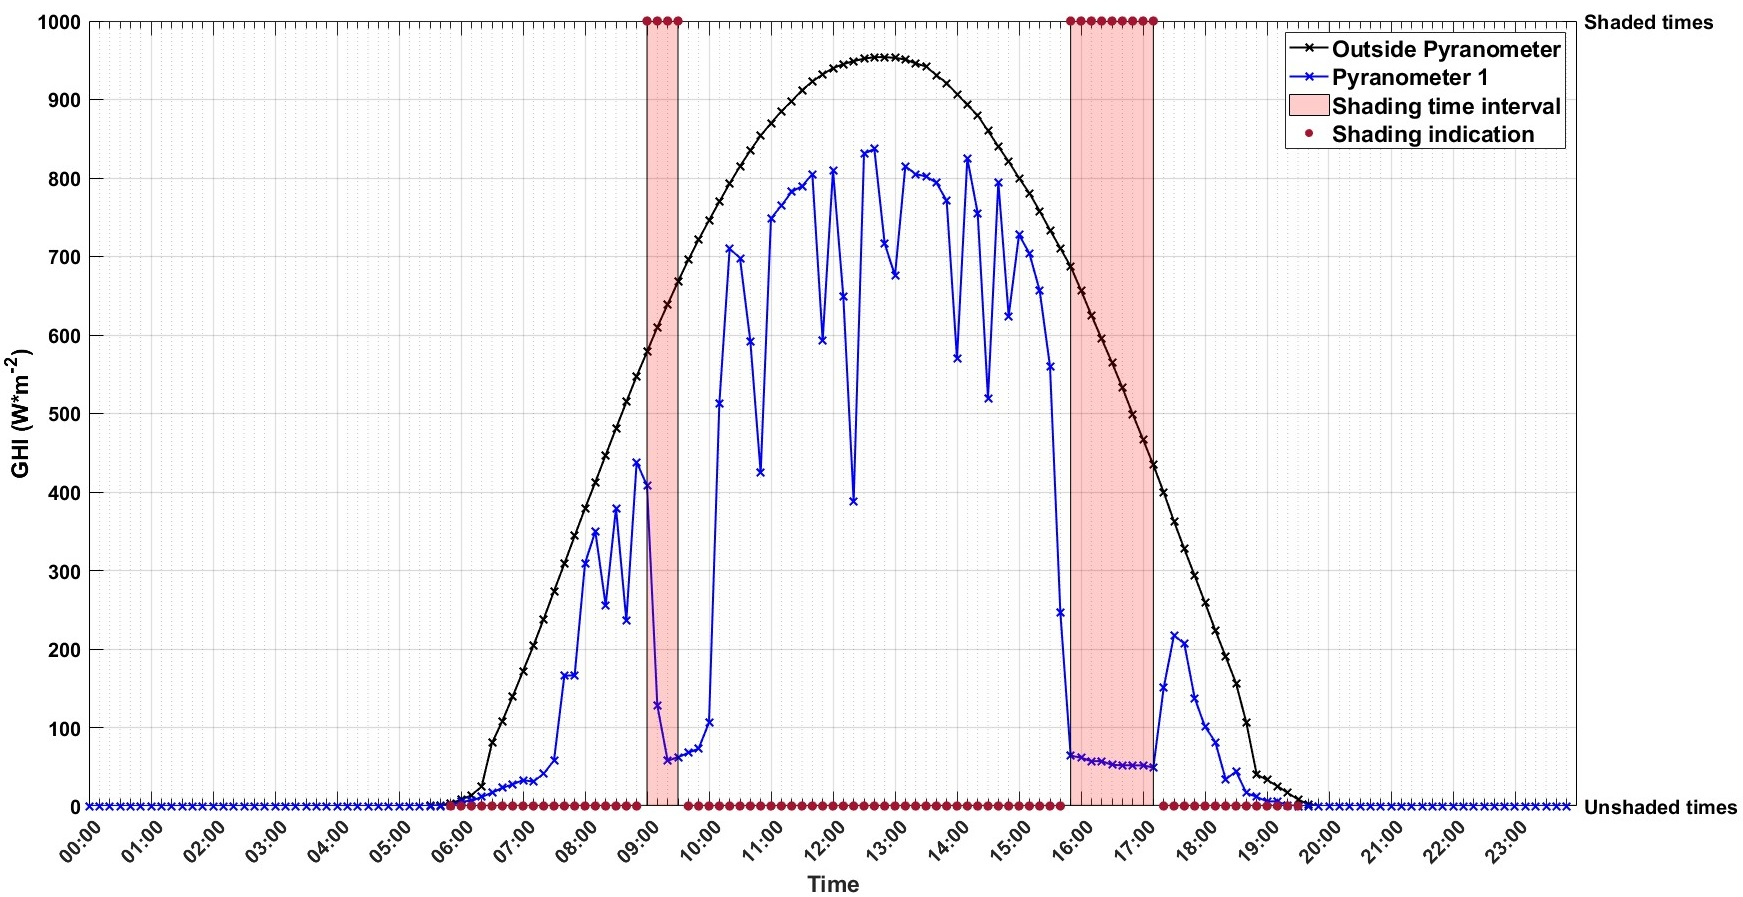
\includegraphics[width=0.9\textwidth]{Figures/GHI_7_8_pyr_1.jpg}
    \caption{Ολική ηλιακή ακτινοβολία σε οριζόντιο επίπεδο και σκίαση για το πυρανόμετρο 1 στις 7 Αυγούστου 2023.}
    \label{fig_GHI_7_8_pyr_1}
\end{figure}

\newpage

\begin{figure}[ht]%
    \centering
    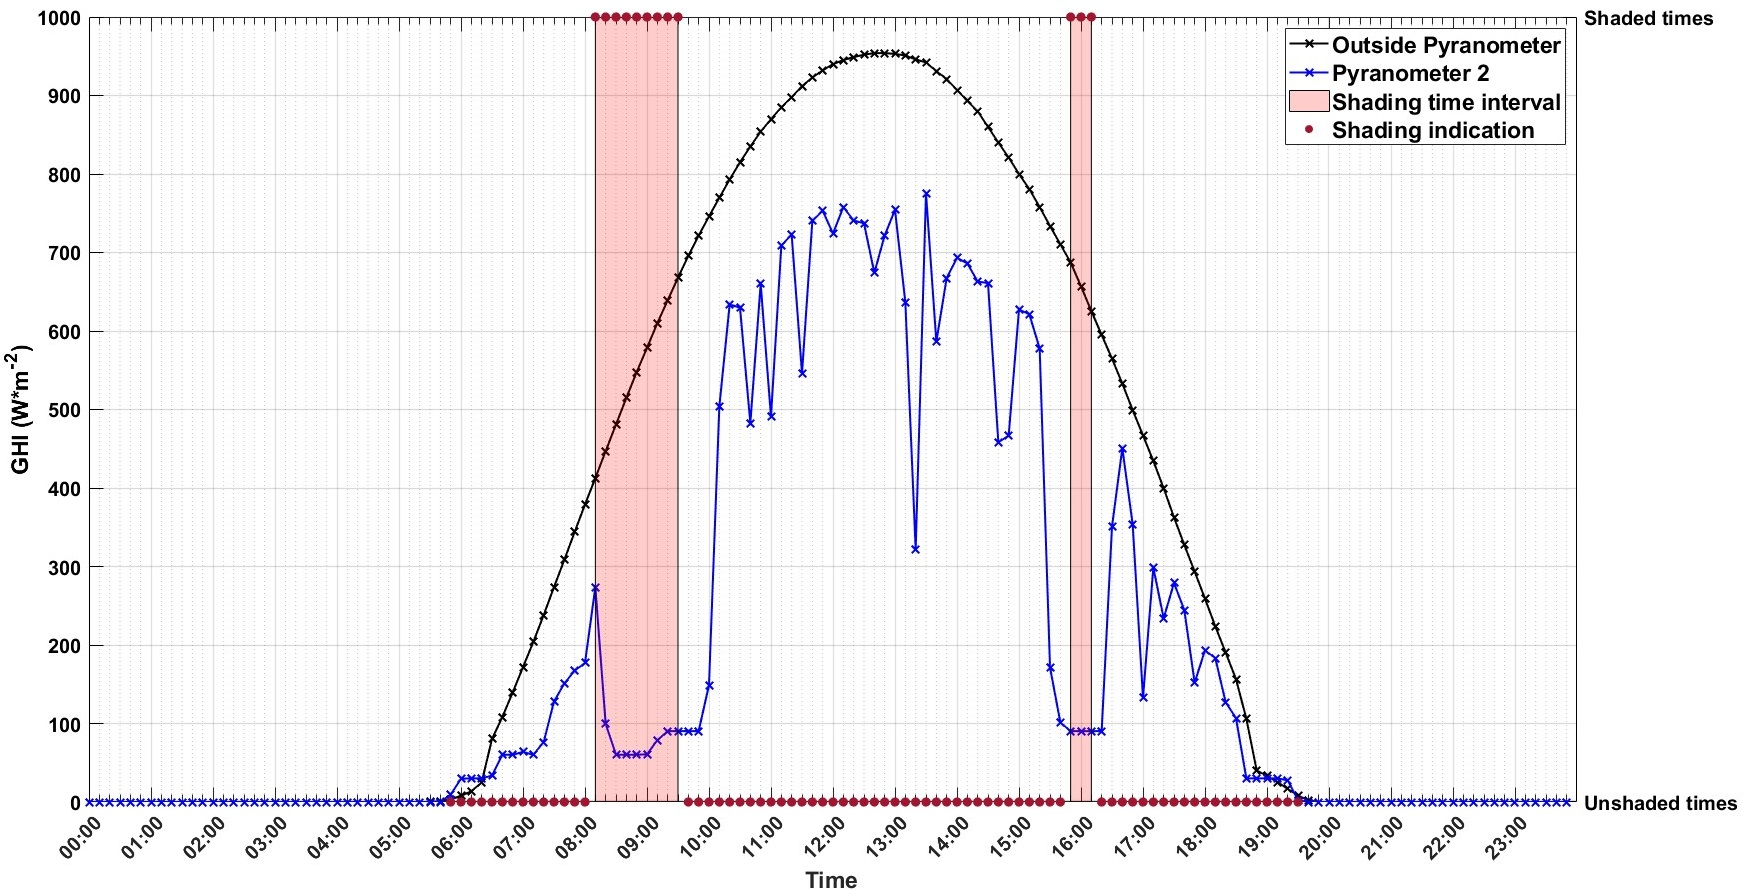
\includegraphics[width=0.9\textwidth]{Figures/GHI_7_8_pyr_2.jpg}
    \caption{Ολική ηλιακή ακτινοβολία σε οριζόντιο επίπεδο και σκίαση για το πυρανόμετρο 2 στις 7 Αυγούστου 2023.}
    \label{fig_GHI_7_8_pyr_2}
\end{figure}

Τα δύο διαφορετικά χρονικά διαστήματα σκίασης οφείλονται, αφενός, στη θέση των πυρανόμετρων εντός του θερμοκηπίου 
(\english{$x_{P,1}$,$y_{P,1}$}) = (4.81,11.85), (\english{$x_{P,2}$,$y_{P,2}$}) = (4.81,4.55), τα οποία είναι 
τοποθετημένα κατά μήκος της ευθείας που χωρίζει το πλάτος της θερμοκηπιακής μονάδας στο μισό, και αφετέρου στην 
κίνηση και το ύψος του ήλιου, η οποία για τη συγκεκριμένη ημέρα και καθώς πλησιάζουμε στο τέλος του έτους γίνεται 
συνεχώς μικρότερη, με αποτέλεσμα η σκιά να μετακινείται προς τα βόρεια, όπως φαίνεται στις Εικόνες \ref{fig_3D_dec}, 
\ref{fig_3D_mar} και \ref{fig_3D_jun}. Βάσει των θέσεων των πυρανόμετρων εξηγείται, ταυτόχρονα, η διακύμανση της 
διάρκειας της σκίασης κατά τις πρωινές και απογευματινές ώρες, αντίστοιχα. Η τοποθέτηση του πυρανόμετρου 1 (Εικόνα 
\ref{fig_GHI_7_8_pyr_1}) στην ανατολική πλευρά του θερμοκηπίου παρουσιάζει μεγαλύτερη χρονικά σκίαση (80 λεπτά) το 
απόγευμα, καθώς ο ήλιος βρίσκεται στα δυτικά του και η σκιά κινείται κυρίως παράλληλα με τον άξονα \english{x} 
(κατεύθυνση βορρά-νότου). Αντίθετα, η σκίαση του κατά τις πρωινές ώρες (30 λεπτά) οφείλεται στο μήκος της φωτοβολταϊκής 
συστοιχίας. Στην περίπτωση του πυρανόμετρου 2 (Εικόνα \ref{fig_GHI_7_8_pyr_2}), το οποίο βρίσκεται στη δυτική πλευρά του 
θερμοκηπίου, η μεγαλύτερη διάρκεια της σκιάς (80 λεπτά) καταγράφεται το πρωί, δηλαδή κατά την ανατολή του ηλίου, ενώ η 
μικρότερη (20 λεπτά) καταγράφεται το απόγευμα.

Όσον αφορά τις τιμές της ακτινοβολίας στα διαστήματα κατά τα οποία τα πυρανόμετρα βρίσκονται εντός της σκιασμένης 
επιφάνειας, παρουσιάζουν μία σχετική συνέπεια, όπως φαίνεται από τις Εικόνες, με τιμές που κυμαίνονται μεταξύ 50 και 
\SI{100}{\watt\per\meter\squared}. Ωστόσο, παρατηρούνται και σημεία που βρίσκονται είτε εντός του παραπάνω εύρους τιμών 
αλλά εκτός σκίασης βάσει του αλγορίθμου, είτε εκτός του παραπάνω εύρους τιμών αλλά εντός της σκιασμένης επιφάνειας. 
Αυτό οφείλεται στο γεγονός ότι, όπως αναφέρεται στην Παράγραφο \ref{subsub_validation}, οι τιμές του πυρανόμετρου είναι 
οι μέσες τιμές των καταγεγραμμένων μονόλεπτων δεδομένων κάθε δέκα λεπτά, σε αντίθεση με τα αποτελέσματα του αλγορίθμου, 
τα οποία παράγουν τη σκίαση κάθε δέκα λεπτά ακριβώς. Έτσι, η εισαγωγή των πυρανόμετρων στη σκιασμένη επιφάνεια στο τέλος 
της χρονικής περιόδου των 10 λεπτών έχει ως αποτέλεσμα μία αυξημένη τιμή της ακτινοβολίας στην περιοχή των 
50-\SI{100}{\watt\per\meter\squared}, ενώ η απουσία σκιάς στο πυρανόμετρο στην αρχή της χρονικής περιόδου των 10 λεπτών 
έχει ως αποτέλεσμα μειωμένη τιμή ακτινοβολίας στο παραπάνω εύρος. Επιπλέον, είναι πιθανό το ενδεχόμενο ότι η σκίαση από 
τον μεγάλο αριθμό των σκελετικών στοιχείων θερμοκηπίου συμπίπτει με τη σκίαση από τα φωτοβολταϊκά.

Η μικρή μεταβολή στην ακτινοβολία, όταν τα δύο πυρανόμετρα είναι σκιασμένα, χρησιμοποιήθηκε για την περαιτέρω επαλήθευση 
του μοντέλου. Όπως αναφέρθηκε στην Παράγραφο \ref{subsub_validation}, η διαφορά μεταξύ της εξωτερικής ακτινοβολίας και 
της ακτινοβολίας που καταγράφηκε από τα δύο πυρανόμετρα προσδιορίστηκε για όλη την περίοδο 05/08/2023 - 29/08/2023, 
προκειμένου να αναλυθεί η “καθαρή” ακτινοβολία εντός του θερμοκηπίου. Ο συντελεστής μεταβλητότητας υπολογίστηκε στη 
συνέχεια τόσο για τους χρόνους που τα πυρανόμετρα ήταν εντός της σκιάς, όσο και για τον υπόλοιπο χρόνο. Στις Εικόνες 
\ref{fig_cv_1} και \ref{fig_cv_2}, παρουσιάζονται οι υπολογισμένοι συντελεστές μεταβλητότητας για καθένα από τα πενήντα 
τυχαία σύνολα δεδομένων με σημεία εκτός της σκιασμένης περιοχής, καθώς και το σύνολο δεδομένων με σημεία όπου το 
πυρανόμετρο είναι σκιασμένο. Τα πενήντα διαφορετικά σύνολα δεδομένων για κάθε ημέρα περιέχουν το ίδιο πλήθος δεδομένων 
με το σύνολο δεδομένων για τη σκιασμένη περιοχή. Ταυτόχρονα, παρέχονται οι τάσεις με βάση τη μέση τιμή τόσο για τα τυχαία, 
όσο και για τα σύνολα δεδομένων που αφορούν την σκιασμένη περιοχή.

\begin{figure}[H]%
    \centering
    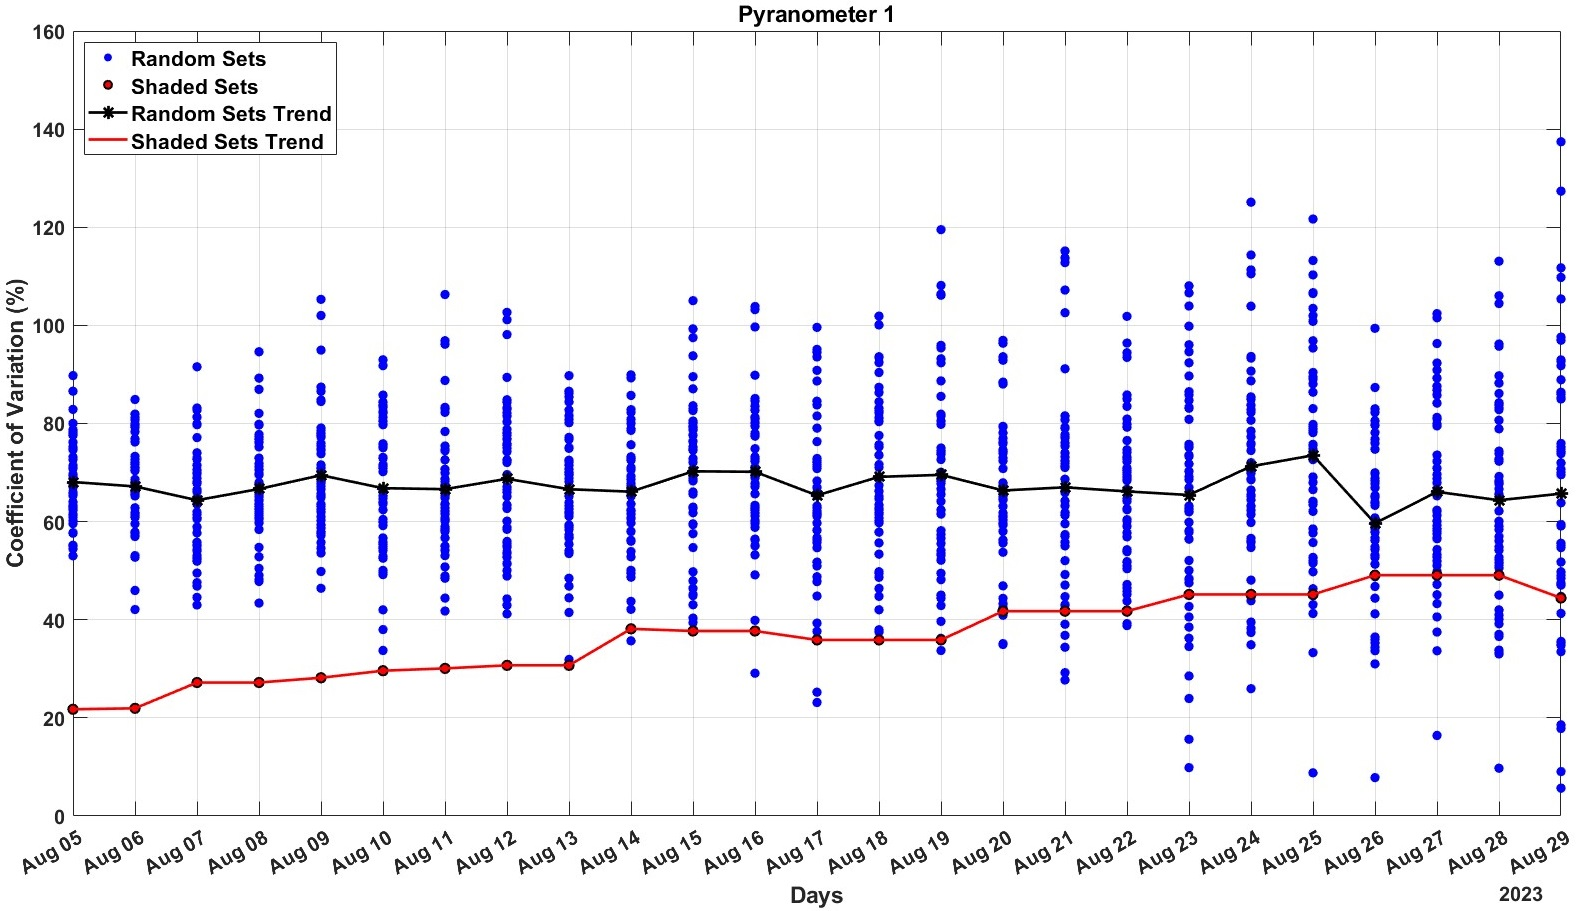
\includegraphics[width=0.9\textwidth]{Figures/cv_1.jpg}
    \caption{Συντελεστές μεταβλητότητας για τα σύνολα δεδομένων της μεταβολής της ακτινοβολίας και οι τάσεις τους για σκιασμένα και μη σκιασμένα σημεία για το πυρανόμετρο 1.}
    \label{fig_cv_1}
\end{figure}

\begin{figure}[H]%
    \centering
    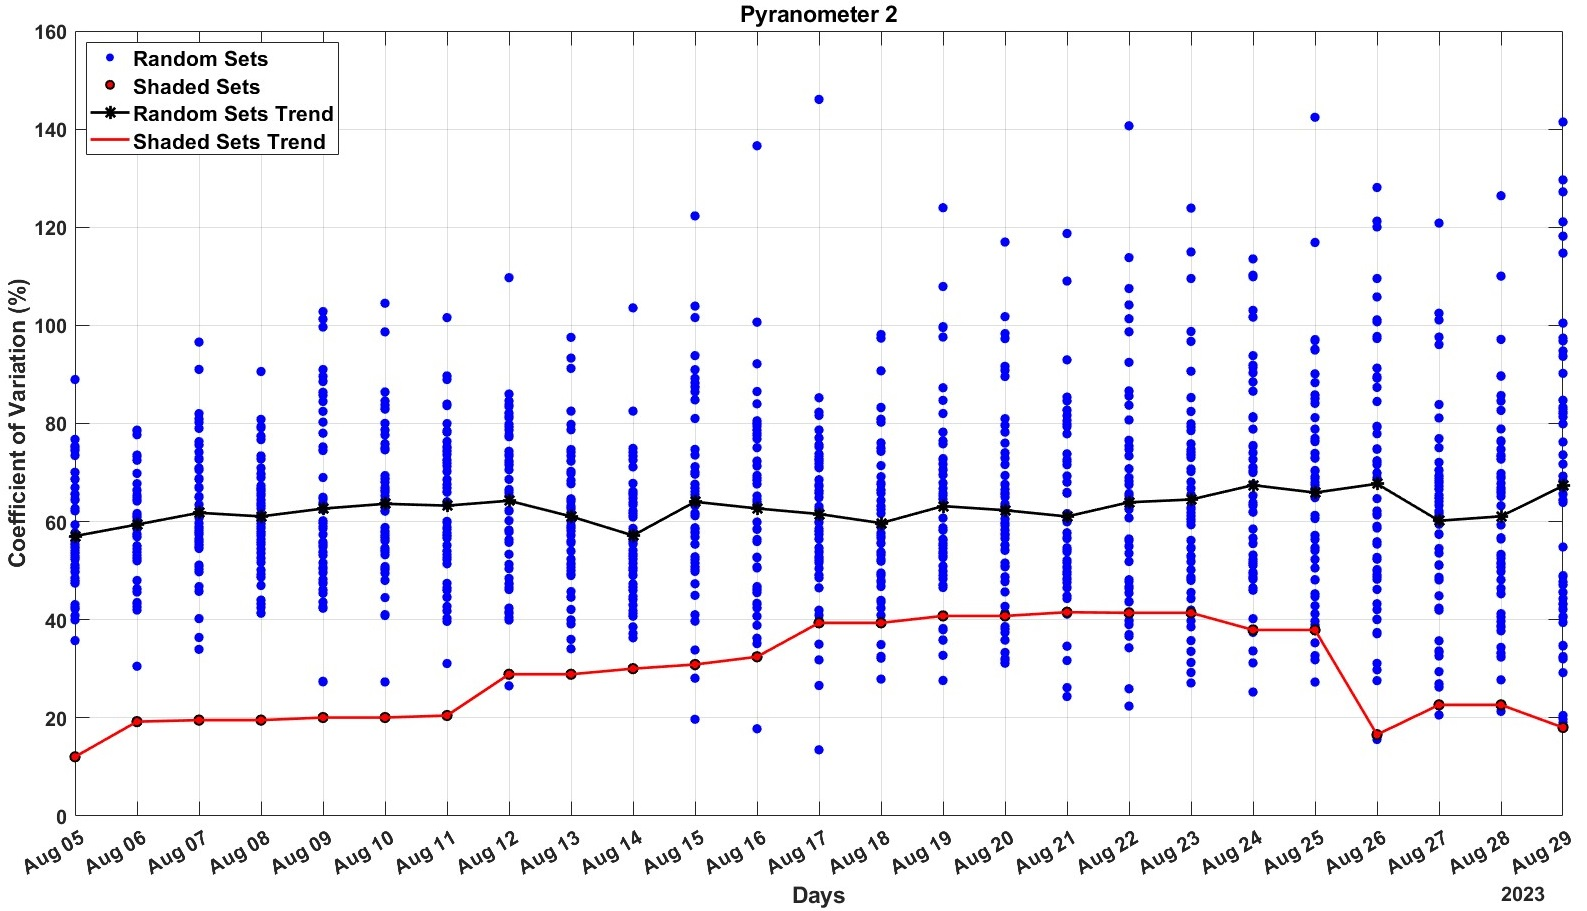
\includegraphics[width=0.9\textwidth]{Figures/cv_2.jpg}
    \caption{Συντελεστές μεταβλητότητας για τα σύνολα δεδομένων της μεταβολής της ακτινοβολίας και οι τάσεις τους για σκιασμένα και μη σκιασμένα σημεία για το πυρανόμετρο 2.}
    \label{fig_cv_2}
\end{figure}

Όπως φαίνεται στις γραφικές παραστάσεις των Εικόνων \ref{fig_cv_1} και \ref{fig_cv_2}, τόσο για το πρώτο όσο και για 
το δεύτερο πυρανόμετρο, η τάση του συντελεστή μεταβλητότητας για τα χρονικά διαστήματα υπό σκιά είναι σταθερά χαμηλότερη 
από την τάση για χρονικά διαστήματα εκτός σκιάς. Αυτό δείχνει ότι η μεταβολή της ακτινοβολίας παραμένει σε πιο σταθερά 
επίπεδα όταν βρίσκεται εντός σκίασης, σε αντίθεση με τις χρονικές στιγμές όπου η μεταβολή της ακτινοβολίας επηρεάζεται 
από την απορρόφηση, τη σκέδαση ή την ανάκλαση από το κάλυμα του θερμοκηπίου. Επιπλέον, η ακτινοβολία μπορεί να 
επηρεάζεται από μεμονωμένες σκιάσεις των σκελετικών στοιχείων του θερμοκηπίου, οι οποίες όμως έχουν μικρή διάρκεια.

Πιο συγκεκριμένα, και όσον αφορά το πυρανόμετρο 1, για τις 11 από τις 25 ημέρες (\SI{44}{\percent}) που εκτελέστηκε 
το πείραμα, ο συντελεστής μεταβλητότητας για το σύνολο δεδομένων με τιμές υπό σκίαση είναι μικρότερος από το 
\SI{100}{\percent} των συντελεστών μεταβλητότητας που αντιστοιχούν στα τυχαία σύνολα δεδομένων που λαμβάνονται χωρίς 
σκίαση, ενώ για 19 από τις 25 ημέρες (\SI{76}{\percent}) ο συντελεστής μεταβλητότητας για το σύνολο δεδομένων με τιμές 
υπό σκίαση είναι μικρότερος από το \SI{90}{\percent} των συντελεστών μεταβλητότητας που αντιστοιχούν στα τυχαία σύνολα 
δεδομένων που λαμβάνονται χωρίς σκίαση. Το ποσοστό αυτό γίνεται ελάχιστο και ισούται με \SI{74}{\percent}, για μία μόνο 
ημέρα. Δηλαδή δεκατρία από τα πενήντα σύνολα δεδομένων όπου δεν υπήρχε σκίαση, παρουσιάζουν μεγαλύτερη ομοιομορφία, 
η οποία οφείλεται στην ύπαρξη νεφοκάλυψης τη συγκεκριμένη ημέρα, αλλά και στη σκίαση που προήλθε από την υδρορροή του 
θερμοκηπίου, όπως παρατηρήθηκε.

Για το πυρανόμετρο 2, ο συντελεστής μεταβλητότητας για το σύνολο δεδομένων με σκιασμένες τιμές είναι μικρότερος από το 
\SI{100}{\percent} των συντελεστών μεταβλητότητας που αντιστοιχούν στα τυχαία σύνολα δεδομένων που λαμβάνονται χωρίς 
σκίαση, για 10 από τις 25 ημέρες (\SI{40}{\percent}) της υπό μελέτη περιόδου, ενώ για 21 από τις 25 ημέρες 
(\SI{84}{\percent}) ο συντελεστής μεταβλητότητας για το σύνολο δεδομένων με σκιασμένες τιμές είναι μικρότερος από το 
\SI{90}{\percent} των συντελεστών μεταβλητότητας που αντιστοιχούν στα τυχαία σύνολα δεδομένων που λαμβάνονται χωρίς 
σκίαση. Το ελάχιστο ποσοστό, όπως και στην προηγούμενη περίπτωση, αντιστοιχεί σε \SI{82}{\percent} με τις αντίστοιχες 
ημέρες κατά τις οποίες συμβαίνει αυτό να είναι 1 στις 25.

Ως αποτέλεσμα των ανωτέρω και με βάση την ομοιομορφία της έντασης της ακτινοβολίας σε σκιασμένη επιφάνεια, διαπιστώνεται 
ότι ο αλγόριθμος εξάγει ικανοποιητικά αποτελέσματα. Ωστόσο, για να διαπιστωθεί η απόλυτη ακρίβεια των αποτελεσμάτων, 
απαιτείται μια πιο εκτεταμένη μελέτη της ακτινοβολίας μέσω πειραμάτων, η οποία αποτελεί επίσης μελλοντική εργασία.

\subsection{Συζήτηση}\label{sub_alg_disc}

Με βάση τον παραπάνω αλγόριθμο, επιτεύχθηκε ο υπολογισμός της σκιάς που προκαλείται από φωτοβολταϊκές μονάδες, 
ενσωματωμένες στο νότιο κεκλιμένο επίπεδο δύο διαφορετικών και παρακείμενων θερμοκηπιακών μονάδων. Αν και τα 
φωτοβολταϊκά είναι ημιδιαφανή, σε αυτή την μελέτη, θεωρήθηκαν αδιαφανή για την εύρεση της σκιάς, με την σκίαση στο έδαφος 
να προκαλείται από ολόκληρη τη μονάδα με βάση τον αλγόριθμο. Οι σχέσεις που χρησιμοποιούνται για την εύρεση της θέσης του 
ήλιου στον ουρανό, σε συνδυασμό με τη χρήση έως και δύο δεκαδικών ψηφίων στις παραμέτρους, δίνουν στον αλγόριθμο τη 
δυνατότητα εξαιρετικά ακριβών αποτελεσμάτων. Παράλληλα, η δημιουργία πινάκων, με σειρές και στήλες που αντιπροσωπεύ\-ουν 
αποστάσεις ενός εκατοστού παρέχει ακόμα μεγαλύτερη ακρίβεια στα αποτελέσματα. Η ακρίβεια αυτή αποδεικνύεται μέσα από τις 
γραφικές αναπαραστάσεις των Εικόνων \ref{fig_diurnal_perc} και \ref{fig_annual_perc}, όπου παρουσιάζονται μικρές, αλλά 
ταυτόχρονα σημαντικές μεταβολές στο ποσοστό κάλυψης του εδάφους του θερμοκηπίου, ανάλογα με τη θέση του ήλιου για κάθε 
διαφορετική περίοδο του έτους.

Τα αποτελέσματα του αλγόριθμου είναι ίδια για κάθε έτος, καθώς η κίνηση του ήλιου υπολογίζεται από αστρονομικές εξισώσεις 
και θεωρίες, ενώ η θερμοκηπιακή μονάδα και οι θέσεις των φωτοβολταϊκών θεωρούνται αμετάβλητες, τόσο χωρικά όσο και 
χρονικά. Ως εκ τούτου, η χρήση του αλγορίθμου θα μπορούσε να γίνει πριν από την κατασκευή του θερμοκηπίου ή την 
εγκατάσταση των φωτοβολταϊκών μονάδων με βάση τα οφέλη ή την επίδραση της σκίασης στην καλλιέργεια.

Αν και ο αλγόριθμος μπορεί να εκτελεστεί μόνο μία φορά για την εξαγωγή των επιθυμητών αποτελεσμάτων, περιορίζεται από 
ορισμένες παραμέτρους. Όπως αναφέρθηκε, η δημιουργία των πινάκων βασίζεται στα εκατοστά ως μονάδα μέτρησης των διαστάσεων. 
Επομένως, για μια θερμοκηπιακή μονάδα μεγάλης έκτασης, το μέγεθος των αντίστοιχων πινάκων θα είναι εξαιρετικά μεγάλο με 
αποτέλεσμα την κάλυψη μεγάλου όγκου υπολογιστικής μνήμης και την αύξηση του χρόνου εκτέλεσης. Ωστόσο, η μείωση δύο 
δεκαδικών ψηφίων σε ένα ή και σε κανένα έχει αρνητική επίδραση στην ακρίβεια των αποτελεσμάτων, ειδικά για μικρές 
θερμοκηπιακές μονάδες. Παράλληλα, αν και οι συναρτήσεις που αφορούν τη δημιουργία του θερμοκηπίου, δίνουν τη δυνατότητα 
εργασίας σε οποιοδήποτε αμφικλινές θερμοκήπιο, η εγκατάσταση των φωτοβολταϊκών περιορίζεται στον τρόπο που έχουν 
τοποθετηθεί τα φωτοβολταϊκά στο συγκεκριμένο θερμοκήπιο, δηλαδή με τη μεγάλη πλευρά τους να ταυτίζεται με τον κορφιά του 
θερμοκηπίου.

Ενώ ο αλγόριθμος αναπτύχθηκε χρησιμοποιώντας προηγούμενες μελέτες και μοντέλα για την εκτίμηση και τον υπολογισμό της 
σκίασης από διαφορετικά αντικείμενα, ένα σημαντικό αποτέλεσμα αυτής της έρευνας είναι ο υπολογισμός της σκίασης που 
προκαλείται από ενσωματωμένα στην οροφή των θερμοκηπίων φωτοβολταϊκά. Επιπλέον, η έρευνα αυτή προσφέρει τη δυνατότητα 
προσδιορισμού της βέλτιστης τοποθέτησης φωτοβολταϊκών για την κάλυψη των απαιτήσεων της καλλιέργειας, γεγονός που αυξάνει 
τη σημασία του.

Όσον αφορά την επικύρωση του μοντέλου, λόγω της μερικής σκίασης που παρέχουν τα ημιδιαφανή φωτοβολταϊκά, απαιτήθηκε ένα 
αδιαφανές κάλυμμα για τη δημιουργία εντονότερης συνεχούς σκίασης. Η συγκεκριμένη πειραματική διάταξη είναι συνεπής με τη 
λειτουργία του αλγορίθμου, ο οποίος θεωρεί τα φωτοβολταϊκά ως αδιαφανείς μονάδες. Λόγω της έντονης σκίασης που παρήχθη, 
τα δύο πυρανόμετρα εντός του θερμοκηπίου κατέγραψαν μια αρκετά σταθερή ένταση ακτινοβολίας κατά τη διάρκεια της περιόδου 
που βρίσκονταν μέσα στην σκιασμένη από τα φωτοβολταϊκά επιφάνεια.

Τα αποτελέσματα του αλγορίθμου παρουσίασαν σχετική συνέπεια ως προς τις τιμές της ακτινοβολίας, ενώ αναμενόμενες ήταν οι 
μετρήσεις που παρουσίαζαν σχετικά μικρές αποκλίσεις λόγω της λειτουργίας των πυρανόμετρων, αφενός με τη χρήση της μέσης 
τιμής των καταγραφών για τα 10λεπτα διαστήματα και αφετέρου λόγω της λειτουργίας του αλγορίθμου, με εξαγωγή αποτελεσμάτων 
αποκλειστικά για κάθε δέκα λεπτά.

Λόγω των παραπάνω, ο συντελεστής μεταβλητότητας υπολογίστηκε με βάση το γεγονός της σχετικά σταθερής ακτινοβολίας εντός 
της σκιασμένης επιφάνειας, ενώ ο υπολογισμός του για την μεταβλή της ακτινοβολίας μεταξύ εξωτερικής και εσωτερικής, έχει 
ως αποτέλεσμα τη μελέτη της “καθαρής” ακτινοβολίας μέσα στο θερμοκήπιο, αφαιρώντας οποιαδήποτε άλλη επίδραση εξωτερικών 
παραγόντων. Ταυτόχρονα, η δημιουργία μεγάλου αριθμού συνόλων δεδομένων (50) για τα μη σκιασμένα χρονικά σημεία καλύπτει 
ολόκληρο το σύνολο των δεδομένων για πιο σαφή αποτελέσματα.

Τέλος, με βάση την τάση των συντελεστών μεταβλητότητας για τα σημεία μέσα και έξω από τη σκιά, παρατηρήθηκε ότι για όλο 
το εύρος της υπό μελέτη χρονικής περιόδου, τα χρονικά σημεία για τα οποία τόσο το πυρανόμετρο 1, όσο και το πυρανόμετρο 
2, βρίσκονται μέσα στη σκιά, δίνουν μια πιο ομοιόμορφη κατανομή της “καθαρής” ακτινοβολίας για τα χρονικά σημεία που 
βρίσκονται στη σκιά με βάση τον αλγόριθμο.

\subsection{Συμπεράσματα}\label{sub_alg_concl}

Τα θερμοκήπια έχουν την δυναμική να αποτελέσουν μια εξαιρετικά βιώσιμη λύση, η οποία όμως περιορίζεται από την υψηλή 
κατανάλωση ενέργειας που τα χαρακτηρίζει. Η λύση της ενσωμάτωσης φωτοβολταϊκών μονάδων στη οροφή του θερμοκηπίου δίνει 
τη δυνατότητα διπλής χρήσης της γης, τόσο με την παραγωγή ενέργειας για την κάλυψη των ενεργειακών αναγκών του ίδιου του 
θερμοκηπίου, όσο και με την παραγωγή τροφίμων. Η σκίαση, ωστόσο, που προκαλείται από τα φωτοβολταϊκά έχει καταλυτική 
επίδραση στο μικροκλίμα και την καλλιέργεια, είτε θετικά είτε αρνητικά, ανάλογα με την εποχή και το είδος της καλλιέργειας.

Σε αυτή την μελέτη παρουσιάζεται ένας αλγόριθμος για τον υπολογισμό της σκιασμένης επιφάνειας από φωτοβολταϊκά μέσα σε 
ένα θερμοκήπιο. Ο αλγόριθμος βασίζεται σε αστρονομικές εξισώσεις και θεωρήματα που αφορούν τη θέση και την κίνηση του 
ήλιου, στη διανυσματική ανάλυση και τη γεωμετρία για την εύρεση της σκιάς, ενώ αποτελείται από πέντε συναρτήσεις και 
τέσσερα τμήματα κώδικα. Τα αποτελέσματα που εξάγονται από τον αλγόριθμο είναι η σκιασμένη επιφάνεια του θερμοκηπίου, το 
ποσοστό του εδάφους που καλύπτεται από την σκιά και δύο γραφικές αναπαραστάσεις του θερμοκηπίου, των φωτοβολταϊκών και 
της σκιάς, μία τρισδιάστατη και μία δισδιάστατη, με τη δεύτερη να παρουσιάζει ουσιαστικά μια κάτοψη της πρώτης.

Με βάση τα αποτελέσματα της επικύρωσης του μοντέλου, αποδεικνύεται ότι ο αλγόριθμος είναι σε θέση να προσδιορίσει τα 
τμήματα του θερμοκηπίου που σκιάζονται από τα φωτοβολταϊκά. Πιο συγκεκριμένα, με βάση τα πειραματικά δεδομένα ακτινοβολίας 
και τη χρήση του συντελεστή μεταβλητότητας, παρατηρήθηκε ακριβής ανίχνευση δεδομένων σκίασης όσον αφορά το πυρανόμετρο 1 
για το \SI{76}{\percent} των ημερών από μια υπό μελέτη περίοδο 29 ημερών, όπου ο συντελεστής μεταβλητότητας για τη 
σκιασμένη περιοχή ήταν μικρότερος από το \SI{90}{\percent} των συντελεστών μεταβλητότητας για σύνολα δεδομένων των μη 
σκιασμένων περιοχών,  επιδεικνύοντας την αναμενόμενη ομοιομορφία της ακτινοβολίας των σκιασμένων περιοχών. Το αντίστοιχο 
ελάχιστο ποσοστό που παρατηρείται είναι ίσο με \SI{74}{\percent} για μία μόνο ημέρα. Παράλληλα, όσον αφορά το πυρανόμετρο 
2, το αντίστοιχο ποσοστό ημερών για τις οποίες παρατηρήθηκε ακριβής ανίχνευση δεδομένων σκίασης φτάνει το \SI{84}{\percent}, 
με το ελάχιστο ποσοστό που παρατηρήθηκε να ισούται με \SI{82}{\percent} για μία μόνο ημέρα. Συνολικά, και με βάση την τάση 
των συντελεστών μεταβλητότητας τόσο για το πυρανόμετρο 1, όσο και για το πυρανόμετρο 2, οι συντελεστές μεταβλητότητας της 
ακτινοβολίας για τις σκιασμένες περιοχές είναι μικρότεροι για όλη την υπό μελέτη περίοδο από τους αντίστοιχους για τις μη 
σκιασμένες περιοχές, υποδεικνύοντας ομοιομορφία της ακτινοβολίας υπό σκίαση και συνεπώς την ύπαρξή της.

Ο αλγόριθμος αυτός θα μπορούσε δυνητικά να αξιοποιηθεί σε Αγριβολταϊκές καλλιέργειες, καθώς υλοποιήθηκε με βάση τις 
ίδιες αρχές, ενώ καλύπτει δεδομένα που αφορούν τη σχέση μεταξύ των δύο βασικών πυλώνων που ορίζουν την έννοια των 
Αγριβολταϊκών, αυτή των φωτοβολταϊκών και αυτή της καλλιέργειας που επηρεάζεται από αυτά. Παράλληλα, αν και ο αλγόριθμος, 
όπως είχε αρχικά σχεδιαστεί, αφορά μόνο θερμοκηπιακές μονάδες, έχει τη δυνατότητα να επεκταθεί και σε ανοικτές 
καλλιέργειες, δυνατότητα που συνάδει με το ευρύτερο πλαίσιο των Αγριβολταϊκών. Ταυτόχρονα, ένα βασικό σημείο που 
χαρακτηρίζει τον αλγόριθμο είναι η δυνατότητά του να αποτελέσει ένα χρήσιμο εργαλείο για τον χρήστη που επιθυμεί 
να εγκαταστήσει φωτοβολταϊκά σε μια θερμοκηπιακή μονάδα, προτείνοντας τη βέλτιστη τοποθέτηση των μονάδων με βάση τη 
σκίαση. Μια σημαντική πτυχή είναι η επιπλέον επικύρωση και επαλήθευση του αλγορίθμου με βάση μετρήσεις ηλιακής 
ακτινοβολίας και αποτελέσματα από άλλες επιστημονικές έρευνες. 

%%%%%%%%%%%%%%%%%%%%%%%%%%%%%%%%%%%%%%%%%%
%%%%%%%%%%%%%%%%%%%%%%%%%%%%%%%%%%%%%%%%%%
\newpage
\vspace*{6.5cm}
\sloppy
\section{Αλγοριθμικές εξελίξεις στα Αγριβολταϊκά: Μοντελοποίηση των επιδράσεων σκίασης από ημιδιαφανή φωτοβολταϊκά}
\label{sec_alg_advanc}
\fussy

Στο παρόν κεφάλαιο, περιγράφονται οι μετατροπές που έγιναν για τη βελτίωση της απόδοσης του αλγορίθμου, καθώς και η δυνατότητα 
επεκτασιμότητάς του σε θερμοκήπια μεγαλύτερης κλίμακας. Επιπλέον, παρουσιάζονται οι τεχνικές που χρησιμοποιήθηκαν για την 
επικύρωση της αναθεωρημένης έκδοσης του αλγορίθμου και τα αποτελέσματά της. Η ακριβής ανίχνευση της σκίασης από ημιδιαφανείς μονάδες 
επιτρέπει πλέον τη χρήση του αλγορίθμου όχι μόνο από επιχειρηματίες και ιδιοκτήτες θερμοκηπίων, αλλά και από μεμονωμένα άτομα 
που επιθυμούν να μελετήσουν με ακρίβεια πρόσθετες παραμέτρους. Οι παράμετροι αυτές μπορεί να αφορούν το μικροκλίμα του θερμοκηπίου, 
όπως η θερμοκρασία, ή βιολογικές παραμέτρους της καλλιέργειας. Αν και ο αλγόριθμος δεν υπολογίζει άμεσα τη διάχυτη ακτινοβολία, 
επιτρέπει την εκτίμησή της χωρίς την ανάγκη πρόσθετων εξειδικευμένων οργάνων. Αυτό μπορεί να επιτευχθεί μόνο με τη μέτρηση της 
ολικής ηλιακής ακτινοβολίας και την αξιοποίηση της ικανότητας του αλγορίθμου να εξετάζει την ηλιακή ακτινοβολία υπό την επίδραση 
διαφόρων περιοχών της φωτοβολταϊκής μονάδας (ηλιακές κυψέλες, διαφανές τμήμα του φωτοβολταϊκού, πλήρης επιφάνεια του φωτοβολταϊκού). 
Επιπλέον, εκτός από τη χωρική ακρίβεια, ο υπολογισμός της σκίασης σε χρονικό βήμα έως και ένα λεπτό παρέχει ακόμη περισσότερες 
ευκαιρίες για έρευνα. Τέλος, μελετάται επίσης η επίδραση των φωτοβολταϊκών τόσο στην \english{GHI} όσο και την \english{PAR}.

Μετά από ανασκόπηση σχετικής βιβλιογραφίας, τα μοντέλα που αναπτύχθηκαν τα τελευταία χρόνια με βάση την έννοια των Αγροβολταϊκών 
αφορούν κυρίως δύο διαφορετικές παραμέτρους, την επίδραση των φωτοβολταϊκών στην ακτινοβολία στο εσωτερικό του θερμοκηπίου και 
άλλες μικροκλιματικές παραμέτρους και την παραγωγή ενέργειας από φωτοβολταϊκά συστήματα σε θερμοκήπια. Πιο συγκεκριμένα, οι
\english{Torrente et al.} (\citeyear{alg_adv_bib1}) δημιούργησαν ένα μοντέλο για την προσομοίωση της κατανομής της ακτινοβολίας 
σε ένα θερμοκήπιο με φωτοβολταϊκά εγκατεστημένα στην οροφή του. Το μοντέλο αυτό, εκτός από την επίδραση των φωτοβολταϊκών στην 
ακτινοβολία, παρέχει επίσης πληροφορίες για την εξατμισοδιαπνοή αναφοράς (\english{$ET_o$}). Από ενεργειακής πλευράς, οι 
\english{Pérez-Alonso et al.} (\citeyear{alg_adv_bib2}) ανέπτυξαν ένα μοντέλο νευρωνικού δικτύου που μπορεί να προβλέψει τη 
στιγμιαία παραγωγή ηλεκτρικής ενέργειας. Τέτοια μοντέλα είναι εξαιρετικά χρήσιμα για πολύπλοκα και μη γραμμικά συστήματα, 
όπως αυτό ενός θερμοκηπίου σε συνδυασμό με ένα φωτοβολταϊκό σύστημα.

\subsection{Βελτιώσεις και τροποποιήσεις}\label{sub_alg_advanc_improves}
Όπως και στο προηούμενο κεφάλαιο της εργασίας, έτσι και σε αυτό, το θερμοκήπιο που χρησιμοποιήθηκε περιγράφεται στην Παράγραφο 
\ref{sub_thermokipio}, ενώ τα φωτοβολταϊκά στην Παράγραφο \ref{sub_PVs}, αντίστοιχα. Ωστόσο, ο αριθμός των φωτοβολταϊκών που 
χρησιμοποιήθηκαν για τις ανάγκες του παρόντος κεφαλαίου είναι 10, με την απομάκρυνση δύο φωτοβολταϊκών μονάδων από τις θέσεις 1 και 2 
της βόρειας κατασκευαστικής μονάδας σύμφωνα με την κατανομή που περιγράφεται στην Παράγραφο \ref{sub_PVs} – “Τοποθέτηση”. Επιπλέον, 
εκτός της χρήσης των πυρανομέτρων των οποίων οι θέσεις εντός του θερμοκηπίου αναφέρονται στην Παράγραφο \ref{subsub_validation}, 
έγινε χρήση δύο μετρητών \english{PAR}, οι οποίοι περιγράφονται στην Παράγραφο \ref{sub_eksoplismos} και βρίσκονται εντός της βόρειας 
κατασκευαστικής μονάδας σε θέσεις με συντεταγμένες (\english{$x_{PAR,1}$,$y_{PAR,1}$}) = (4.71,11.85) και 
(\english{$x_{PAR,2}$,$y_{PAR,2}$}) = (4.71,4,55).

Όπως αναφέρεται και στο Κεφάλαιο \ref{sec_algorithm}, ο αρχικός αλγόριθμος δεν λάμβανε υπόψη την ημιδιαφάνεια των φωτοβολταϊκών. 
Αντ' αυτού, οι μονάδες θεωρούνταν αδιαφανείς, με την σκίαση να υπολογίζεται ως μία συνεχής επιφάνεια στο έδαφος. Αν και αυτή η 
προσέγγιση μπορεί να καλύψει ένα ευρύ φάσμα σεναρίων Αγριβολταϊκών σε θερμοκήπια, καθώς τα φωτοβολταϊκά που χρησιμοποιούνταν μέχρι 
πριν λίγα χρόνια ήταν κυρίως αδιαφανή, δεν μπορεί να παρέχει ακριβή αποτελέσματα για τη συγκεκριμένη περίπτωση των ημιδιαφανών 
φωτοβολταϊκών, τα οποία αποτελούν μία ευρέως διαδεδομένη λύση τα τελευταία χρόνια. Ως εκ τούτου, ήταν απαραίτητο να μοντελοποιηθούν 
τα φωτοβολταϊκά, όχι ως μια συνεχής και αδιαφανής επιφάνεια, αλλά ως μια επιφάνεια με αδιαφανείς ηλιακές κυψελίδες ενσωματωμένες 
σε συγκεκριμένα σημεία. Ο αλγόριθμος, συνεπώς, βελτιώθηκε λαμβάνοντας υπόψη τη σκίαση που προκαλείται όχι από τη συνολική επιφάνεια 
του φωτοβολταϊκού, αλλά από τις ηλιακές κυψελίδες του. Στην Εικόνα \ref{fig_opaque_vs_semitr}, αριστερά απεικονίζεται η επιφάνεια 
του φωτοβολταϊκού, όπως αρχικά προβλεπόταν (αδιαφανής – \english{opaque}) και δεξιά όπως λαμβάνεται υπόψη στο παρόν κεφάλαιο 
(ημιδιαφανής – \english{semi-transparent}).

\begin{figure}[H]
    \centering
    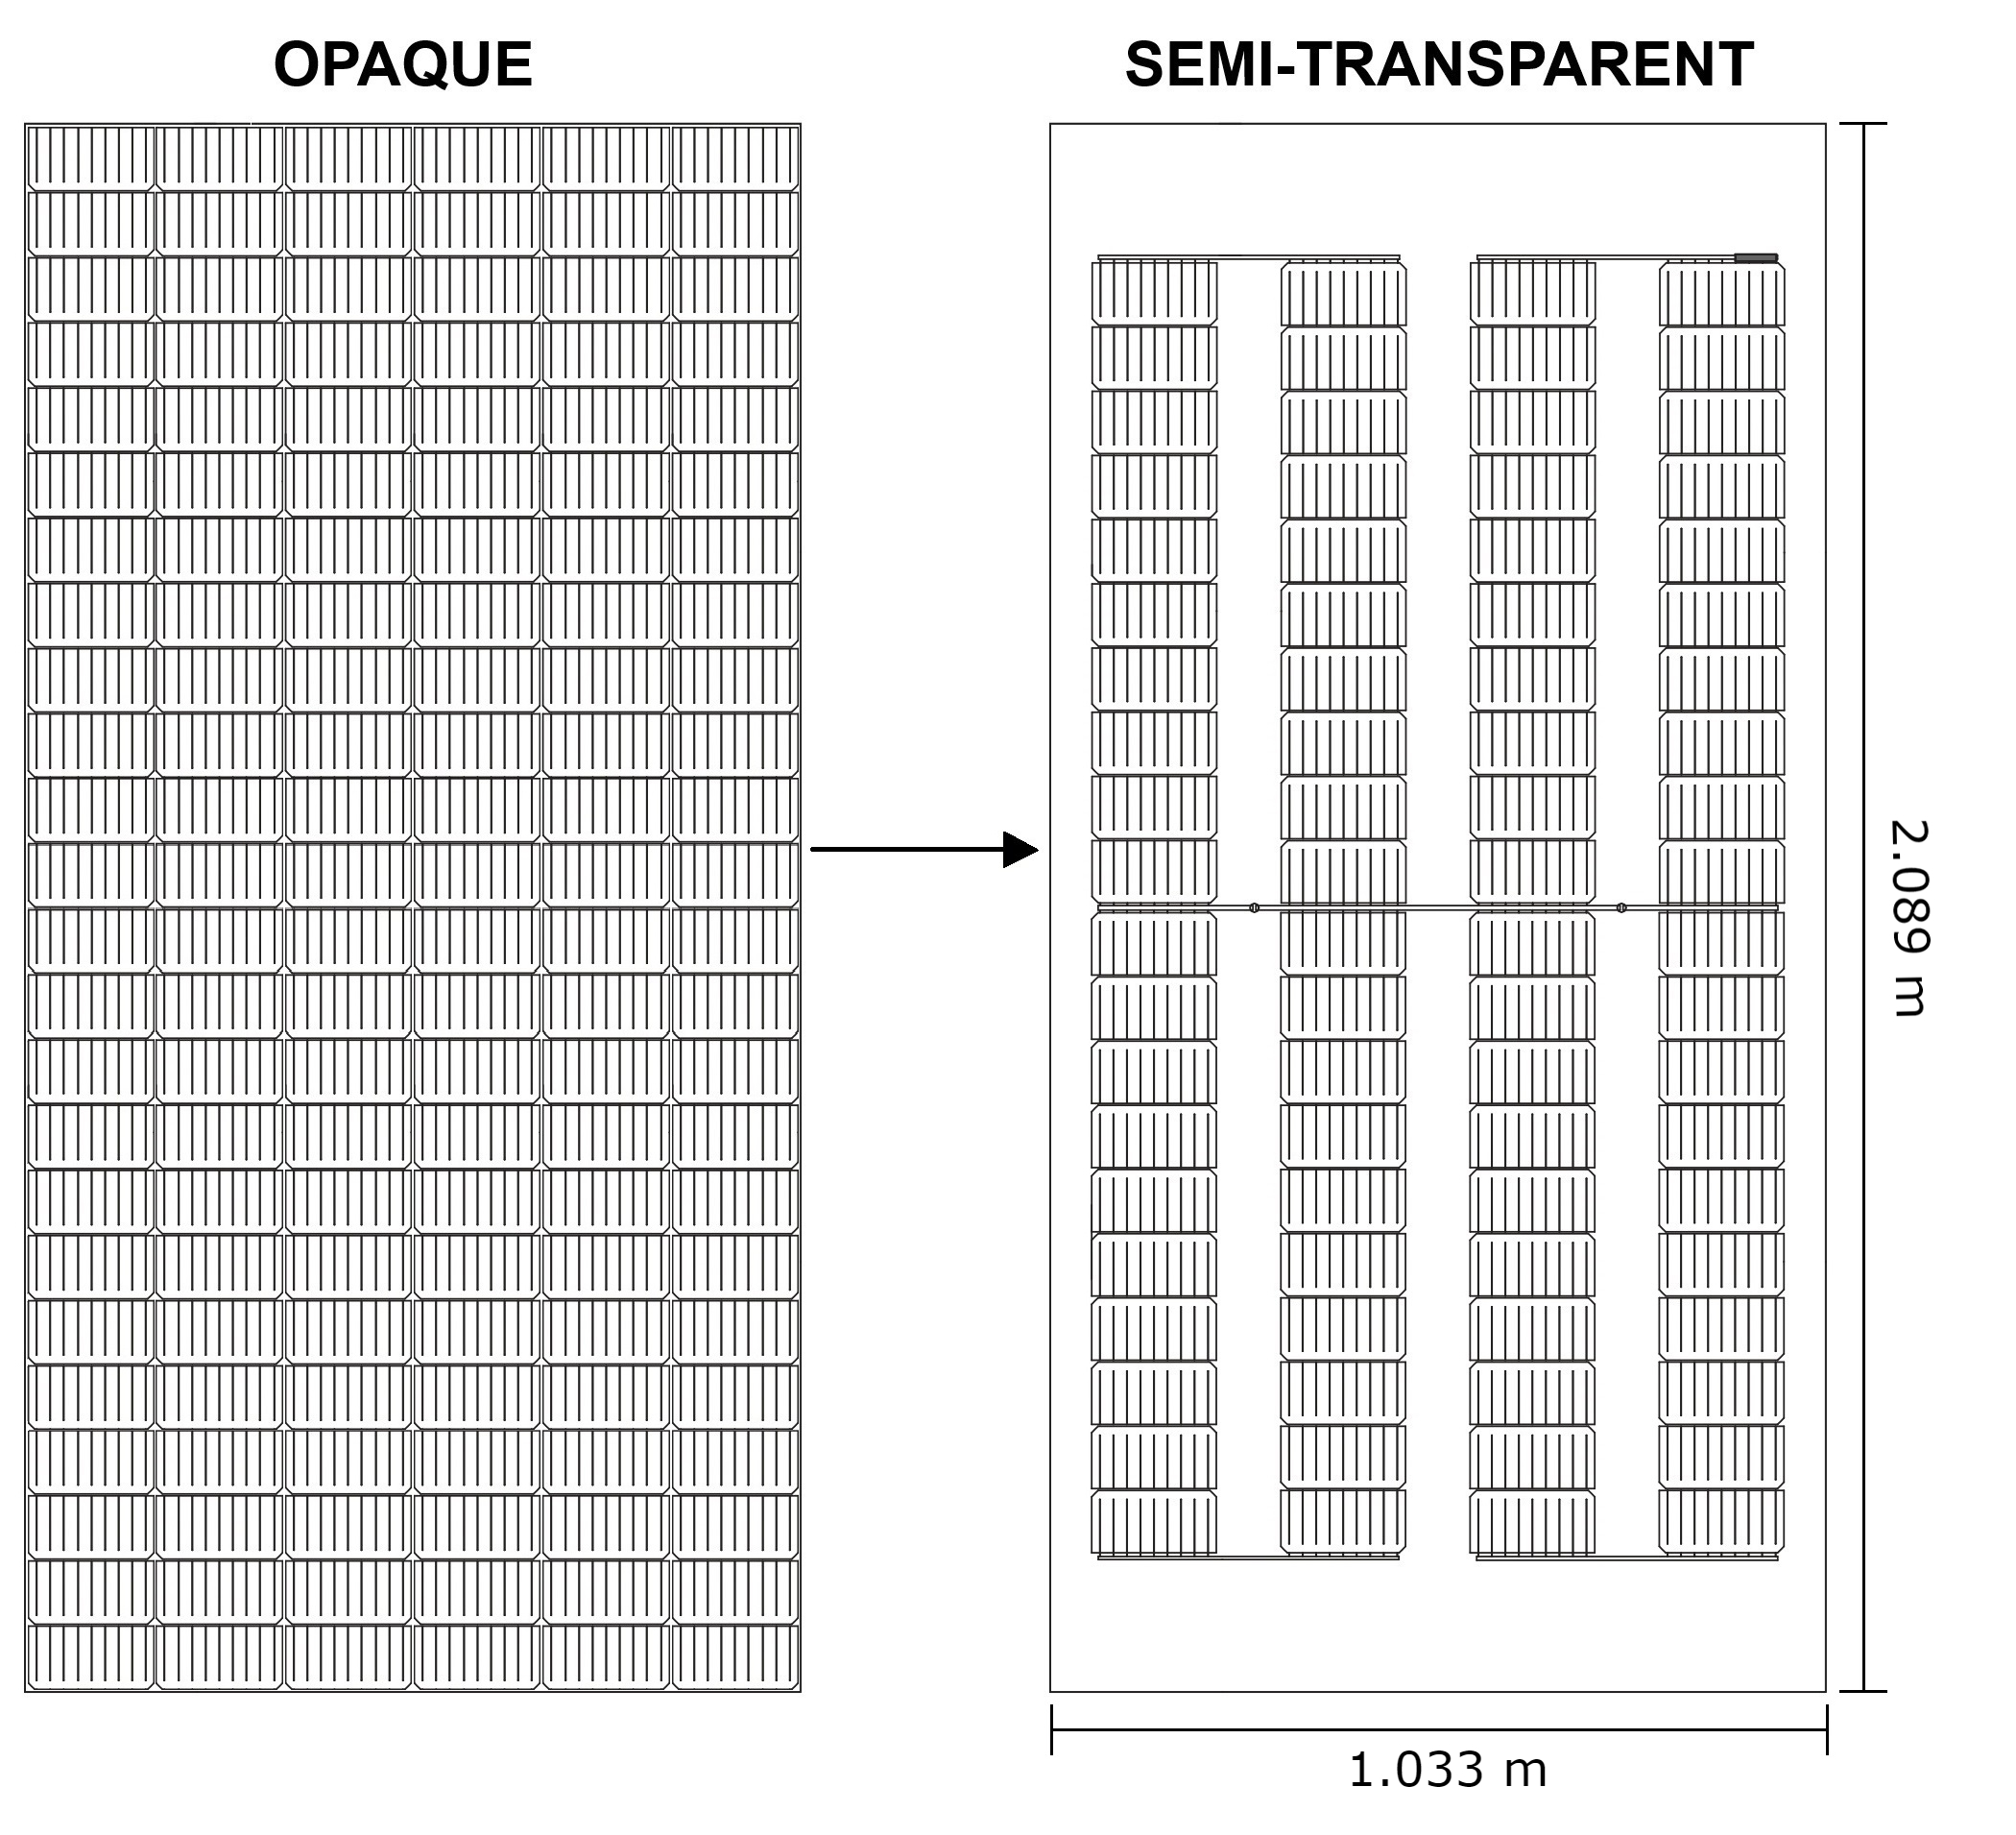
\includegraphics[width=.8\linewidth]{OP_ST_PVS_updated.jpg}
    \caption{Φωτοβολταϊκές μονάδες ως αδιαφανής επιφάνεια (αριστερά) και ως ημιδιαφανής επιφάνεια (δεξιά) \lcitep{strawberries_bib17}}
    \label{fig_opaque_vs_semitr}
\end{figure}

Η μεθοδολογία για τον υπολογισμό των συντεταγμένων των ηλιακών κυψελίδων σε Καρτεσιανό σύστημα συντεταγμένων είναι η ίδια με 
εκείνη που χρησιμοποιείται για την εύρεση των συντεταγμένων της φωτοβολταϊκής μονάδας. Kάθε φωτοβολταϊκή μονάδα αποτελείται 
από ογδόντα ηλιακά κύτταρα ομοιόμορφα κατανεμημένα σε τέσσερις γραμμές των είκοσι ηλιακών κυψελίδων. Έτσι, στον υπάρχοντα κώδικα 
προστέθηκαν τμήματα για τον υπολογισμό τεσσάρων τριπλετών συντεταγμένων (\english{$x$,$y$,$z$}) για κάθε γραμμή (μία για κάθε 
γωνία του ορθογωνίου που σχηματίζεται από τις κυψέλες), με αποτέλεσμα να προκύψουν τελικά δεκαέξι τιμές για τον άξονα \english{x}, 
δεκαέξι τιμές για τον άξονα \english{y} και δεκαέξι τιμές για τον άξονα \english{z}. Αυτές οι τριπλέτες συντεταγμένων 
υπολογίζονται για κάθε φωτοβολταϊκή μονάδα ενσωματωμένη στην οροφή του θερμοκηπίου. 

Στο Καρτεσιανό σύστημα συντεταγμένων, κάθε άξονας αντιπροσωπεύει μια κατεύθυνση του θερμοκηπίου. Λαμβάνοντας υπόψη ότι η μεγάλη 
πλευρά του θερμοκηπίου είναι παράλληλη προς την κατεύθυνση Ανατολή-Δύση, ο άξονας \english{x} του συστήματος αντιπροσωπεύει την 
κατεύθυνση Βορρά-Νότου, η κατεύθυνση Ανατολή-Δύση αντιστοιχεί στον άξονα \english{y}, ενώ ο άξονας \english{z} αντιπροσωπεύει την 
κατακόρυφη απόσταση από την επιφάνεια. Χρησιμοποιώντας βρόχους επανάληψης “\english{for}”, υπολογίζονται όλες οι απαραίτητες 
συντεταγμένες ως προς τον αριθμό των κατασκευαστικών μονάδων που επαναλαμβάνονται κατά πλάτος (δείκτης \english{$i$}) και κατά 
μήκος (δείκτης \english{$m$}), τον αριθμό των φωτοβολταϊκών μονάδων (δείκτης \english{$j$}) και τον αριθμό των γραμμών ηλιακών 
κυψελίδων (δείκτης \english{$t$}). Το Τμήμα του Κώδικα 1 του Παραρτήματος \ref{appx_A_5} – Κεφάλαιο 5 παρουσιάζει ενδεικτικό 
κώδικα που προστέθηκε στον αρχικό αλγόριθμο για τον υπολογισμό των συντεταγμένων των γραμμών ηλιακών κυψελίδων.

Μια ακόμη παράμετρος που τροποποιήθηκε στον αλγόριθμο είναι το χρονικό βήμα βάσει του οποίου ο αλγόριθμος μπορεί να υπολογίσει 
τη σκιασμένη επιφάνεια. Στην αρχική του μορφή, ο αλγόριθμος υπολόγιζε τη σκίαση μέχρι ένα ελάχιστο βήμα 10 λεπτών. Προσθέτοντας 
μια παράμετρο για τα λεπτά στην εξίσωση κλασματικού έτους (Εξίσωση \ref{eq_gamma}), είναι πλέον δυνατή η εύρεση της σκίασης 
μέχρι ένα ελάχιστο βήμα χρόνου 1 λεπτού. Πιο συγκεκριμένα, η αρχικά χρησιμοποιούμενη Εξίσωση \ref{eq_gamma}, μετατρέπεται στην 
Εξίσωση \ref{eq_gamma_updated}. Ταυτόχρονα, τροποποιούνται οι χρονικοί περιορισμοί, με τον περιορισμό 
\texttt{\english{Minute = [0:10:50]}} να γίνεται \texttt{\english{Minute = [0:1:59]}}.

\begin{equation}
    \english{\gamma = \frac{2\pi}{365} \left( N - 1 + \frac{h - 12 + \frac{mnt}{24}}{24}\right)}
    \label{eq_gamma_updated}
\end{equation}

\noindent όπου \textit{γ} είναι το κλασματικό έτος (\english{rad}), \english{$N$} είναι η ημέρα του έτους, η οποία κυμαίνεται 
μεταξύ 1 και 365 ή 366 (για δίσεκτα έτη), και \english{$h$} και \english{$mnt$} είναι η επιθυμητή ώρα και το λεπτό της ημέρας, 
αντίστοιχα.

Ένα βήμα χρόνου του 1 λεπτού είναι ιδιαίτερα σύντομο, καθώς τέτοιες βραχυπρόθεσμες μεταβολές στην ηλιακή ακτινοβολία δεν 
επηρεάζουν σημαντικά την τελική παραγωγή βιομάζας. Τέτοιες μεταβολές είναι αξιοσημείωτες σε περιπτώσεις όπου η ακτινοβολία 
μεταβάλλεται λόγω σκίασης για τουλάχιστον μία ώρα εντός 24 ωρών. Ωστόσο, οι ημερήσιες διακυμάνσεις της ηλιακής ακτινοβολίας 
μπορεί να συμβούν μέσα σε δευτερόλεπτα λόγω ατμοσφαιρικών παραμέτρων όπως τα σύννεφα. Ανάλογα με το είδος του φυτού, τα 
στομάτια προσαρμόζονται στις μεταβολές των αβιοτικών παραμέτρων μέσα σε λίγα δευτερόλεπτα ή λεπτά, από τη στιγμή της εμφάνισης 
του στρεσογόνου παράγοντα \lcitep{alg_adv_bib3,alg_adv_bib4}. Από την άλλη πλευρά, για φυτά των οποίων οι προσαρμογές των 
στομάτων είναι πιο αργές, με χρονικές κλίμακες μεγαλύτερες από τις αβιοτικές παραμέτρους, αυτές οι αλλαγές θα μπορούσαν να 
οδηγήσουν σε μαρασμό του φυτού \lcitep{alg_adv_bib5}.

Έτσι, αν και στην παρούσα έρευνα, το μικρότερο χρονικό βήμα για τον προσδιορισμό της σκιάς προοριζόταν για τη διερεύνηση 
της ηλιακής ακτινοβολίας με μεγαλύτερη ακρίβεια, ο αλγόριθμος θα μπορούσε πλέον να χρησιμοποιηθεί και για τη μελέτη 
αντιδράσεων που σχετίζονται με βιοχημικούς και βιοφυσικούς φυσιολογικούς μηχανισμούς, από τους οποίους εξαρτώνται διάφορες 
φωτοσυνθετικές λειτουργίες, καθώς και τις προσαρμογές των στομάτων.

Όπως αναφέρεται και στο Κεφάλαιο \ref{sec_algorithm}, κάθε συνάρτηση ή μέρος του κώδικα λαμβάνει ως είσοδο την έξοδο της 
προηγούμενης συνάρτησης ή μέρους του κώδικα. Επομένως, αλλάζοντας το χρονικό βήμα για τον υπολογισμό της σκίασης, 
απαιτείται μια μικρή αλλά σημαντική τροποποίηση στη συνάρτηση που υπολογίζει την απόσταση Γης-Ήλιου (Συνάρτηση 2 του 
Παραρτήματος \ref{appx_A_4} – Κεφάλαιο 4). Δεδομένου ότι η Γη απαιτεί 365 ημέρες για μια πλήρη περιστροφή \SI{365}{\degree}, σε μία 
ημέρα, η γωνία που καλύπτει είναι ίση με \SI{0,986}{\degree}. Έτσι, για ένα χρονικό διάστημα 1 λεπτού, η γωνία ισούται με 
\SI{0,986}{\degree\per1440}, όπου 1440 είναι τα χρονικά διαστήματα ενός λεπτού σε μια ημέρα. Αυτή η γωνία χρησιμοποιείται 
για να βρεθούν οι συντεταγμένες (\english{$x$,$y$}), οι οποίες αντιστοιχούν στη θέση της Γης στην τροχιά της γύρω από τον Ήλιο.

Ταυτόχρονα, μια σημαντική πρόσθετη δυνατότητα είναι ο υπολογισμός της σκιασμένης επιφάνειας σε διάφορα ύψη. Ειδικά κατά τις 
πρωινές και απογευματινές ώρες, όταν η Ηλιακή Ζενίθια Γωνία λαμβάνει υψηλές τιμές, η διαφορά στη θέση της σκιάς όσον αφορά 
το ύψος είναι σημαντική. Έτσι, τα πυρανόμετρα που βρίσκονται σε ύψη μεγαλύτερα από \SI{0,5}{\meter} ενδέχεται να μην καταγράφουν 
ακριβείς τιμές ακτινοβολίας, ιδίως όταν πλησιάζουν τα άκρα της σκιασμένης περιοχής. Εκτός από τη διασφάλιση ακριβών μετρήσεων 
ακτινοβολίας στην παρούσα μελέτη, είναι πλέον δυνατό, μέσω πολλαπλών εκτελέσεων του αλγορίθμου, να γίνει πλήρης χαρτογράφηση της 
σκίασης σε όλο τον όγκο του θερμοκηπίου, γεγονός που θα είναι επίσης επωφελές για καλλιέργειες μεγάλου ύψους.

Πιο συγκεκριμένα, στις εξισώσεις που υπολογίζουν τις συντεταγμένες της σκιασμένης επιφάνειας (Εξισώσεις \ref{eq_x_shadow} 
και \ref{eq_y_shadow}), έχει προστεθεί ένας επιπλέον παράγοντας για το επιθυμητό ύψος της σκιάς, \english{$z_{sh}$}. Η τιμή 
αυτή παρέχεται ως αρχική μεταβλητή εισόδου στον αλγόριθμο, με τις αρχικές εξισώσεις να μετατρέπονται στις Εξισώσεις 
\ref{eq_x_shadow_modified} και \ref{eq_y_shadow_modified}. Με την επίλυση αυτών των εξισώσεων προκύπτουν τελικά σύνολα 
συντεταγμένων (\english{$x$,$y$,$z$}) που αντιστοιχούν στις κορυφές της σκιασμένης επιφάνειας.

\begin{equation}
    \english{x_{sh, modified} = x_n - c_n \cdot \left(z_n - z_{sh}\right)}
    \label{eq_x_shadow_modified}
\end{equation}

\begin{equation}
    \english{y_{sh, modified} = y_n - \frac{\left(z_n - z_{sh}\right)}{b_n}}
    \label{eq_y_shadow_modified}
\end{equation}

\noindent όπου (\english{$x_{sh,modified}$,$y_{sh,modified}$}) είναι οι τροποποιημένες συντεταγμένες σκιάς σε σχέση με το 
επιθυμητό ύψος σκιάς, \english{$x_n$, $y_n$} και \english{$z_n$}, είναι οι συντεταγμένες που ορίζουν κάθε γωνία του φωτοβολταϊκού, 
με $n$ = 1, 2, 3, 4, και \english{$b_n$} και \english{$c_n$} δύο παράμετροι που δίνονται από τις Εξισώσεις \ref{eq_b_n} και 
\ref{eq_c_n}, αντίστοιχα.

Ένα μέρος του κώδικα που παρουσίασε προβλήματα στον αρχικό αλγόριθμο ήταν η δυαδική ανάλυση (Παράγραφος \ref*{subsub_binary_analysis}). 
Η δημιουργία πινάκων με λογικές τιμές για την αναπαράσταση τόσο του θερμοκηπίου όσο και της σκιάς καθυστερεί την εκτέλεση του 
αλγορίθμου, καθιστώντας τον λιγότερο αποδοτικό. Η αναπαράσταση κάθε τετραγωνικού εκατοστού (λόγω της επιθυμητής υψηλής ακρίβειας) 
ως κελί ενός πίνακα, είχε ως αποτέλεσμα τη δημιουργία πινάκων με σημαντικά μεγάλο μέγεθος, ακόμη και για ένα θερμοκήπιο που 
καλύπτει μικρή έκταση. Πρέπει να σημειωθεί ότι ο αλγόριθμος σχεδιάστηκε για να λειτουργεί για οποιοδήποτε θερμοκήπιο, ανεξάρτητα 
από τον αριθμό των κατασκευαστικών μονάδων και το μέγεθός τους. Επομένως, για ένα υπερμεγέθες εμπορικό θερμοκήπιο, θα ήταν ιδιαίτερα 
δύσχρηστος. Επιπλέον, τμήματα του αλγορίθμου έχουν απομονωθεί έτσι ώστε ο αλγόριθμος να εκτελεί πολλαπλές εκτελέσεις, εξάγοντας 
όλα τα αποτελέσματα εκτός από τις γραφικές αναπαραστάσεις. Σε αυτήν την περίπτωση, η δημιουργία πολλαπλών μεγάλων πινάκων απαιτούσε 
τεράστια υπολογιστική ισχύ και μνήμη.

Για τους παραπάνω λόγους, το τμήμα της δυαδικής ανάλυσης αντικαταστάθηκε με μια μέθοδο που λειτουργεί με βάση την εντολή 
\english{“boundary”} στη γλώσσα προγραμματισμού \english{MATLAB}. Με τη συγκεκριμένη εντολή, αρκεί να βρεθούν μόνο τα σημεία που 
αποτελούν είτε το έδαφος που καλύπτεται από το θερμοκήπιο είτε τη σκιασμένη επιφάνεια, σημεία δηλαδή που υπολογίστηκαν από τις 
προηγούμενες συναρτήσεις. Έτσι, αποφεύγεται πλέον η δημιουργία πρόσθετων πινάκων, ενώ η ακρίβεια εξαρτάται από τον αριθμό των 
δεκαδικών ψηφίων που ορίζει ο χρήστης. Στο Τμήμα του Κώδικα 2 του Παραρτήματος \ref{appx_A_5} – Κεφάλαιο 5 παρουσιάζεται 
ενδεικτικά ο κώδικας που προστέθηκε στον αρχικό αλγόριθμο για τον υπολογισμό όλων των απαιτούμενων επιφανειών, καθώς και των 
σκιασμένων επιφανειών από το σύνολο των φωτοβολταϊκών μονάδων και των ηλιακών κυψελίδων.

Η δημιουργία πινάκων με λογικές τιμές ήταν επίσης η βάση για τον έλεγχο του κατά πόσον ένα δεδομένο σημείο (συγκεκριμένες 
συντεταγμένες) βρίσκεται εντός της σκιασμένης επιφάνειας. Η μέθοδος αυτή βασιζόταν στο γεγονός ότι οι γραμμές των πινάκων 
αντιπροσώπευαν σημεία κατά μήκος του άξονα \english{y} και οι στήλες των πινάκων αντιπροσώπευαν σημεία κατά μήκος του άξονα \english{x}. 
Έτσι, εάν τόσο η συντεταγμένη \english{x} όσο και η συντεταγμένη \english{y} του δεδομένου σημείου ήταν εντός του εύρους των στηλών 
που λάμβαναν τιμές 1 (υποδηλώνοντας την παρουσία σκιάς), τότε το σημείο ανήκε στη σκιασμένη επιφάνεια. Διαφορετικά, το σημείο 
βρισκόταν εκτός.

Η μέθοδος αυτή αντικαταστάθηκε από μια πιο απλουστευμένη προσέγγιση, σύμφωνα με την οποία ένα σημείο βρίσκεται εντός μιας 
δεδομένης περιοχής, εάν το άθροισμα των επιφανειών που δημιουργούνται μεταξύ του σημείου και κάθε κορυφής ενός πολυγώνου είναι 
ίσο με τη συνολική επιφάνεια του πολυγώνου. Σε περίπτωση που το άθροισμα των επιφανειών είναι μεγαλύτερο, τότε το σημείο βρίσκεται 
εκτός της επιθυμητής επιφάνειας. Πιο συγκεκριμένα, και σύμφωνα με την Εικόνα \ref{fig_methods}α, για να βρίσκεται ένα δεδομένο 
σημείο \english{$I$} εντός της περιοχής \english{$ABCD$}, το άθροισμα των επιφανειών \english{$AIC$} (\english{$E_1$}), 
\english{$AIB$} (\english{$E_2$}), \english{$BID$} (\english{$E_3$}) και \english{$DIC$} (\english{$E_4$}) πρέπει να είναι ίσο 
με το εμβαδόν της \english{$ABCD$}, όπως περιγράφεται από την Εξίσωση \ref{eq_meth_in}. Σύμφωνα με την Εικόνα \ref{fig_methods}β, 
ένα δεδομένο σημείο \english{$I$} βρίσκεται εκτός της περιοχής \english{$ABCD$} όταν το άθροισμα των περιοχών \english{$AIC$} 
(\english{$E_1$}), \english{$AIB$} (\english{$E_2$}), \english{$BID$} (\english{$E_3$}) και \english{$DIC$} (\english{$E_4$}) είναι 
μεγαλύτερο από την περιοχή \english{$ABCD$}, όπως περιγράφεται από την Eξίσωση \ref{eq_meth_out}. Το Τμήμα του Κώδικα 3 του 
Παραρτήματος \ref{appx_A_5} – Κεφάλαιο 5 παρουσιάζει ενδεικτικό κώδικα της παραπάνω μεθόδου που χρησιμοποιήθηκε.

\begin{equation}
    E_1 + E_2 + E_3 + E_4 = E_{ABCD}
    \label{eq_meth_in}
\end{equation}

\begin{equation}
    E_1 + E_2 + E_3 + E_4 > E_{ABCD}
    \label{eq_meth_out}
\end{equation}

\begin{figure}[H]
    \begin{minipage}[c]{.5\textwidth}
\centering
      \includegraphics[width=0.9\linewidth]{method_in.jpg}
      \caption*{\hspace{35pt}(α)}{}
    \end{minipage}%
    \begin{minipage}[c]{0.5\textwidth}
\centering
      \includegraphics[width=0.9\linewidth]{method_out.jpg}
      \caption*{\hspace{35pt}(β)}{}
    \end{minipage}
\caption{Μέθοδος προσδιορισμού της θέσης ενός σημείου: (α) το σημείο βρίσκεται εντός της επιθυμητής επιφάνειας, (β) το σημείο 
βρίσκεται εκτός της επιθυμητής επιφάνειας.}
\label{fig_methods}
\end{figure}

\subsection{Μέθοδος επικύρωσης του αλγορίθμου}\label{sub_alg_advanc_valid}

Ο αρχικός αλγόριθμος επικυρώθηκε χρησιμοποιώντας πραγματικά δεδομένα ηλιακής ακτινοβολίας που καταγράφηκαν με τη χρήση τριών 
ίδιων πυρανόμετρων (\english{CMP3} της \english{Kipp \& Zonen}). Τα δύο ήταν τοποθετημένα στο εσωτερικό του θερμοκηπίου για την 
καταγραφή της ακτινοβολίας που διαπερνούσε το κάλυμμα και τα φωτοβολταϊκά, ενώ το τρίτο ήταν έξω από το θερμοκήπιο για την 
καταγραφή της προσπίπτουσας στο θερμοκήπιο ακτινοβολίας. Ο συντελεστής στον οποίο βασίστηκε η επικύρωση ήταν ο συντελεστής 
μεταβλητότητας. Με βάση αυτόν, και λόγω του σχετικά σταθερού μεγέθους της διαφοράς μεταξύ 
εξωτερικής και εσωτερικής ακτινοβολίας (\english{$GHI_{external}$ – $GHI_{internal}$}), όταν το πυρανόμετρο βρισκόταν εντός της 
σκιασμένης περιοχής που προσδιορίστηκε από τον αλγόριθμο, αποδείχθηκε η ορθότητα των αποτελεσμάτων.

Στην παρούσα μελέτη, χρησιμοποιήθηκε η ίδια μέθοδος για την επικύρωση της αναθεωρημένης έκδοσης του αλγόριθμου, χρησιμοποιώντας 
συγκεκριμένα τον συντελεστή μεταβλητότητας, ενώ παράλληλα χρησιμοποιήθηκε και ο συντελεστής συσχέτισης \english{Pearson’s r}).

Ο συντελεστής συσχέτισης \english{Pearson’s r} εξετάζει κατά πόσον τα δεδομένα σχετίζονται μεταξύ τους, με τις ακραίες δυνατές 
τιμές -1 και +1 να υποδηλώνουν τέλεια αρνητική και θετική γραμμική συσχέτιση, αντίστοιχα. Αντίθετα, μια τιμή του συντελεστή ίση 
με μηδέν υποδηλώνει ότι δεν υπάρχει συσχέτιση μεταξύ των δεδομένων. Ο συντελεστής \english{Pearson’s r} υπολογίζεται από την 
Εξίσωση \ref{eq_pearsons}. Από την άλλη πλευρά, ο συντελεστής μεταβλητότητας ορίζεται ως ο λόγος μεταξύ της τυπικής απόκλισης ($\sigma$)
και της μέσης τιμής ($\mu$) (Εξίσωση \ref{eq_CV}), ο οποίος επιτρέπει τη συσχέτιση αυτών των δύο παραμέτρων, και έτσι την ανίχνευση 
οποιωνδήποτε διακυμάνσεων. Πιο συγκεκριμένα, ο συντελεστής μεταβλητότητας συνήθως εκφράζεται ως ποσοστό, με τις μικρές τιμές να 
υποδεικνύουν μικρότερες μεταβολές στα δεδομένα.

\begin{equation}
    r = \frac{\sum_{i=1}^{n} (x_i - \bar{x})(y_i - \bar{y})}{\sqrt{\sum_{i=1}^{n} (x_i - \bar{x})^2} \sqrt{\sum_{i=1}^{n} (y_i - \bar{y})^2}}
    \label{eq_pearsons}
\end{equation}

\begin{equation}
    CV = \left( \frac{\sigma}{\mu} \right) \times 100\%
    \label{eq_CV}
\end{equation}

Στη μελέτη αυτή χρησιμοποιήθηκαν μονόλεπτα δεδομένα από εννέα διαφορετικές καθαρές ημέρες κατά το τρίμηνο Απριλίου-Μαΐου-Ιουνίου 
2024. Τα δεδομένα πριν την ανατολή και μετά τη δύση του ηλίου απορρίφθηκαν, λόγω της αδυναμίας του αλγόριθμου να υπολογίσει τη 
θέση του ήλιου αυτές τις ώρες και συνεπώς την σκίαση. Κατά συνέπεια, ο συνολικός αριθμός των δεδομένων που χρησιμοποιήθηκαν 
ήταν 7598.

Για να προσδιοριστεί η σκιασμένη επιφάνεια που προκαλείται από τα φωτοβολταϊκά, ο αλγόριθμος εκτελέστηκε για καθεμία από τις υπό 
μελέτη ημέρες, χρησιμοποιώντας τα χαρακτηριστικά του θερμοκηπίου, των φωτοβολταϊκών μονάδων και των ηλιακών κυψελών, λαμβάνοντας 
επίσης υπόψη τις θέσεις και το ύψος των δύο πυρανομέτρων. Τα αποτελέσματα του αλγορίθμου που χρησιμοποιήθηκαν για την επικύρωση 
του αλγορίθμου ήταν τα χρονικά διαστήματα κατά τα οποία τα πυρανόμετρα 1 και 2 ήταν:

\begin{enumerate}[label=(\english{\alph*$_r$})]
    \item εντός και εκτός της επίδρασης της συνολικής επιφάνειας των φωτοβολταϊκών μονάδων της βόρειας κατασκευαστικής μονάδας,
    \item εντός και εκτός της επίδρασης της σκιάς που σχηματίζουν οι ηλιακές κυψέλες των αντίστοιχων φωτοβολταϊκών μονάδων,
    \item εντός της επίδρασης του “διαφανούς” τμήματος των αντίστοιχων φωτοβολταϊκών μονάδων.
\end{enumerate}

Οι παραπάνω περιπτώσεις περιγράφονται επίσης στην Εικόνα \ref{fig_valid_fig}. Για την περίπτωση (\english{$a_r$}), όταν τα 
πυρανόμετρα βρίσκονται εντός της επίδρασης της συνολικής επιφάνειας των φωτοβολταϊκών μονάδων, βάσει της Εικόνας \ref{fig_valid_fig}, 
τα πυρανόμετρα βρίσκονται είτε εντός της κόκκινης είτε εντός της πράσινης περιοχής. Διαφορετικά, τα πυρανόμετρα βρίσκονται 
οπουδήποτε αλλού (λευκός χώρος). Για την περίπτωση (\english{$b_r$}), όταν τα πυρανόμετρα βρίσκονται εντός της σκιάς που 
σχηματίζουν οι ηλιακές κυψελίδες, βρίσκονται εντός της κόκκινης περιοχής. Διαφορετικά, βρίσκονται είτε εντός της πράσινης είτε 
οπουδήποτε αλλού. Τέλος, για την περίπτωση (\english{$c_r$}), όταν τα πυρανόμετρα βρίσκονται εντός της επίδρασης του “διαφανούς” 
τμήματος των φωτοβολταϊκών, βρίσκονται εντός της πράσινης περιοχής της Εικόνας \ref{fig_valid_fig}.

\begin{figure}[H]
    \centering
    \includegraphics[width=.6\linewidth]{valid_fig.jpg}
    \caption{Σκιά που σχηματίζεται από τις φωτοβολταϊκές μονάδες της βόρειας κατασκευαστικής μονάδας: (α) η κόκκινη περιοχή 
    αντιστοιχεί στη σκιά που σχηματίζουν οι ηλιακές κυψέλες, (β) η πράσινη περιοχή αντιστοιχεί στην επίδραση του “διαφανούς” 
    τμήματος των φωτοβολταϊκών μονάδων. Ο λευκός χώρος δεν επηρεάζεται από τα φωτοβολταϊκά.}
    \label{fig_valid_fig}
\end{figure}

Για κάθε ένα από τα πέντε σύνολα δεδομένων, υπολογίστηκαν οι συντελεστές συσχέτισης \english{Pearson’s r} μεταξύ της ηλιακής 
ακτινοβολίας εκτός του θερμοκηπίου και της ηλιακής ακτινοβολίας από τα πυρανόμετρα 1 και 2. Επιπλέον, υπολογίστηκαν τα 
\english{p-values} με επίπεδο σημαντικότητας 0,05 για την αξιολόγηση της στατιστικής σημαντικότητας των αποτελεσμάτων. Σε 
συνδυασμό με τα παραπάνω, οι αντίστοιχοι συντελεστές συσχέτισης υπολογίστηκαν για εννέα καθαρές ημέρες κατά την ίδια περίοδο 
το έτος 2022, όταν οι φωτοβολταϊκές μονάδες δεν είχαν ακόμη εγκατασταθεί στο θερμοκήπιο. Αυτό θα παράσχει μια σχετική εικόνα 
της σχέσης μεταξύ της ηλιακής ακτινοβολίας έξω και μέσα στο θερμοκήπιο χωρίς την επίδραση των φωτοβολταϊκών. Οι θέσεις των 
πυρανόμετρων παρέμειναν σταθερές και για τα δύο έτη, 2022 και 2024.

Όσον αφορά τον συντελεστή μεταβλητότητας, η διαφορά μεταξύ της ηλιακής ακτινοβολίας έξω από το θερμοκήπιο και της ηλιακής 
ακτινοβολίας από τα πυρανόμετρα 1 και 2 εντός του θερμοκηπίου, υπολογίστηκε από τα καταγεγραμμένα αντίστοιχα δεδομένα. 
Με βάση και πάλι τα αποτελέσματα του αλγορίθμου, τα δεδομένα χωρίστηκαν σύμφωνα με τις ακόλουθες περιπτώσεις:

\begin{enumerate}[label=(\english{\alph*$_{cv}$})]
    \item Τα πυρανόμετρα ήταν εκτός της επίδρασης της συνολικής επιφάνειας των φωτοβολταϊκών μονάδων της βόρειας κατασκευαστικής 
    μονάδας (4570 μετρήσεις για το πυρανόμετρο 1 και 5794 για το πυρανόμετρο 2).
    \item Τα πυρανόμετρα ήταν εντός της επίδρασης της συνολικής επιφάνειας των φωτοβολταϊκών μονάδων της βόρειας κατασκευαστικής 
    μονάδας (3028 μετρήσεις για το πυρανόμετρο 1 και 1804 για το πυρανόμετρο 2).
    \item Τα πυρανόμετρα ήταν εντός της επίδρασης της σκίασης που δημιουργούσαν οι ηλιακές κυψελίδες (1936 μετρήσεις για το 
    πυρανόμετρο 1 και 1171 για το πυρανόμετρο 2).
    \item Τα πυρανόμετρα ήταν εντός της επίδρασης του “διαφανούς” τμήματος των αντίστοιχων φωτοβολταϊκών μονάδων (1092 μετρήσεις 
    για το πυρανόμετρο 1 και 633 για το πυρανόμετρο 2).
\end{enumerate}

Για τον υπολογισμό των \english{CV} και τη σύγκριση των συντελεστών της περίπτωσης \english{($a_{cv}$)} με τους συντελεστές των 
περιπτώσεων \english{($b_{cv}$)}, \english{($c_{cv}$)} και \english{($d_{cv}$)}, και δεδομένου ότι ο αριθμός των δεδομένων 
λαμβάνεται υπόψη από το \english{CV}, για το πυρανόμετρο 1 τα δεδομένα της περίπτωσης \english{($a_{cv}$)} χωρίστηκαν σε:

\begin{itemize}
    \item 20 τυχαία μικρότερα σύνολα δεδομένων που επιλέχθηκαν για σύγκριση με τον \english{CV} της περίπτωσης \english{($b_{cv}$)}
    \item 30 τυχαία μικρότερα σύνολα δεδομένων που επιλέγονται για σύγκριση με τον \english{CV} της περίπτωσης \english{($c_{cv}$)}
    \item 50 τυχαία μικρότερα σύνολα δεδομένων που επιλέγονται για σύγκριση με τον \english{CV} της περίπτωσης \english{($d_{cv}$)}
\end{itemize}

\noindent ενώ για το Πυρανόμετρο 2 τα δεδομένα της περίπτωσης \english{($a_{cv}$)} χωρίστηκαν σε:

\begin{itemize}
    \item 40 τυχαία μικρότερα σύνολα δεδομένων που επιλέχθηκαν για σύγκριση με τον \english{CV} της περίπτωσης \english{($b_{cv}$)}
    \item 50 τυχαία μικρότερα σύνολα δεδομένων που επιλέγονται για σύγκριση με τον \english{CV} της περίπτωσης \english{($c_{cv}$)}
    \item 100 τυχαία μικρότερα σύνολα δεδομένων που επιλέγονται για σύγκριση με τον \english{CV} της περίπτωσης \english{($d_{cv}$)}
\end{itemize}

Η επιλογή του αριθμού των μικρότερων συνόλων δεδομένων έγινε διαιρώντας τον αριθμό των δεδομένων της περίπτωσης \english{($a_{cv}$)} 
με τον αριθμό των δεδομένων της κάθε μίας από τις περιπτώσεις \english{($b_{cv}$)}, \english{($c_{cv}$)} και \english{($d_{cv}$)}, 
αντίστοιχα, και τα αποτελέσματα αυτά πολλαπλασιάστηκαν επί 10 για να καλυφθούν όσο το δυνατόν περισσότεροι συνδυασμοί.

\subsection{Αποτελέσματα και συζήτηση}\label{sub_alg_advanc_results}
\subsubsection{Αποτελέσματα επικύρωσης του αλγορίθμου}\label{sub_alg_advanc_valid_results}

Όπως αναφέρθηκε παραπάνω, για την επικύρωση του αλγορίθμου χρησιμοποιήθηκαν δύο διαφορετικοί συντελεστές, αφενός ο συντελεστής 
συσχέτισης \english{Pearson’s r} και αφετέρου ο συντελεστής μεταβλητότητας. Η επικύρωση πραγματοποιήθηκε εκτελώντας τον αλγόριθμο 
για οκτώ καθαρές ημέρες, τρεις από τον Απρίλιο (20 Απριλίου 2024, 28 Απριλίου 2024, 29 Απριλίου 2024), τέσσερις από τον Μάιο 
(06 Μαΐου 2024, 22 Μαΐου 2024, 28 Μαΐου 2024) και τρεις από τον Ιούνιο (01 Ιουνίου 2024, 21 Ιουνίου 2024, 22 Ιουνίου 2024).

Στις Εικόνες \ref{fig_GHI_data}α, γ και ε παρουσιάζονται ενδεικτικά τα δεδομένα για τις 29 Απριλίου 2024, 28 Μαΐου 2024 και 22 
Ιουνίου 2024 για το πυρανόμετρο 1, ενώ στις Εικόνες \ref{fig_GHI_data}β, δ και ζ παρουσιάζονται τα αντίστοιχα δεδομένα για το 
πυρανόμετρο 2. Πιο συγκεκριμένα, στα παρακάτω γραφήματα παρουσιάζονται η εξωτερική ακτινοβολία, η εσωτερική ακτινοβολία που 
καταγράφεται από τα πυρανόμετρα και τα αποτελέσματα του αλγορίθμου. Οι κόκκινες περιοχές υποδεικνύουν τις περιόδους κατά 
τις οποίες το πυρανόμετρο βρίσκεται, σύμφωνα με τον αλγόριθμο, εντός της σκιασμένης περιοχής που σχηματίζουν οι ηλιακές 
κυψελίδες, ενώ οι πράσινες περιοχές υποδεικνύουν τις περιόδους κατά τις οποίες το πυρανόμετρο βρίσκεται υπό την επίδραση 
μόνο του “διαφανούς” τμήματος των φωτοβολταϊκών.

Στον Πίνακα \ref{tab_pearsons_r} παρουσιάζονται οι τιμές των συντελεστών συσχέτισης που υπολογίστηκαν για τις περιπτώσεις όπου τα 
πυρανόμετρα βρίσκονται υπό την επίδραση ή όχι ολόκληρης της επιφάνειας των φωτοβολταϊκών μονάδων (περιπτώσεις \english{a1} 
και \english{a2}), τα πυρανόμετρα βρίσκονται υπό την επίδραση ή όχι της σκίασης που σχηματίζουν οι ηλιακές κυψελίδες των 
φωτοβολταϊκών μονάδων (περιπτώσεις \english{b1} και \english{b2}) και την περίπτωση όπου τα πυρανόμετρα βρίσκονται υπό την 
επίδραση του “διαφανούς” τμήματος των φωτοβολταϊκών (περίπτωση \english{c}). Όλα τα αντίστοιχα \english{p-values} σε επίπεδο 
σημαντικότητας 0,05 είναι ίσα με 0, με αποτέλεσμα τη στατιστική σημαντικότητα των αποτελεσμάτων.

% \newpage

\begin{figure}[H]
    \begin{adjustwidth}{-0.7cm}{0cm}
        \begin{minipage}{0.5\textwidth}
            \centering
            \includegraphics[scale=0.085]{29_Apr_GHI_1.jpg}
            \caption*{\hspace{35pt}(α)}{}
        \end{minipage}
        \hfill
        \begin{minipage}[c]{0.5\textwidth}
            \centering
            \includegraphics[scale=0.085]{29_Apr_GHI_2.jpg}
            \caption*{\hspace{35pt}(β)}{}
        \end{minipage}

        \medskip

        \begin{minipage}[c]{0.5\textwidth}
            \centering
            \includegraphics[scale=0.085]{28_May_GHI_1.jpg}
            \caption*{\hspace{35pt}(γ)}{}
        \end{minipage}
        \hfill
        \begin{minipage}[c]{0.5\textwidth}
            \centering
            \includegraphics[scale=0.085]{28_May_GHI_2.jpg}
            \caption*{\hspace{35pt}(δ)}{}
        \end{minipage}

        \medskip

        \begin{minipage}[c]{0.5\textwidth}
            \centering
            \includegraphics[scale=0.085]{21_Jun_GHI_1.jpg}
            \caption*{\hspace{35pt}(ε)}{}
        \end{minipage}
        \hfill
        \begin{minipage}[c]{0.5\textwidth}
            \centering
            \includegraphics[scale=0.085]{21_Jun_GHI_2.jpg}
            \caption*{\hspace{35pt}(στ)}{}
        \end{minipage}
    \end{adjustwidth}
    \caption{Εξωτερική \english{GHI}, εσωτερική \english{GHI} και αποτελέσματα αλγορίθμου για τις 29 Απριλίου 2024, 28 Μαΐου 2024 
    και 21 Ιουνίου 2024, καταγεγραμμένα από (α), (γ), (ε) το πυρανόμετρο 1, (β), (δ), (στ) το πυρανόμετρο 2. (Κόκκινες περιοχές: 
    περίοδοι κατά τις οποίες το πυρανόμετρο βρίσκεται εντός της σκιασμένης περιοχής που σχηματίζουν οι ηλιακές κυψελίδες. 
    Πράσινες περιοχές: περίοδοι κατά τις οποίες το πυρανόμετρο είναι υπό την επίδραση μόνο του “διαφανούς” τμήματος των 
    φωτοβολταϊκών.)}
    \label{fig_GHI_data}
\end{figure}

\newpage

\begin{table}[ht]
    \centering
    \caption{Συντελεστές συσχέτισης μεταξύ των διαφορετικών περιπτώσεων σκίασης ή μη των πυρανόμετρων 1 και 2.}
    \label{tab_pearsons_r}
        \begin{tabular}{>{\centering\arraybackslash}m{7.5cm} >{\centering\arraybackslash}m{7.5cm}}
        \toprule
        \textbf{Περίπτωση}	& \textbf{Τιμή \english{Pearson's r}}\\
        \midrule
        \multicolumn{2}{c}{\textbf{Πυρανόμετρο 1}} \\
        \midrule
        \english{a1} & 0,2602 \\
        \english{a2} & 0,9188 \\ 
        \english{b1} & 0,2550 \\
        \english{b2} & 0,8179 \\
        \english{c} & 0,3408 \\
        \midrule
        \multicolumn{2}{c}{\textbf{Πυρανόμετρο 2}} \\
        \midrule
        \english{a1} & 0,3261 \\
        \english{a2} & 0,8751 \\ 
        \english{b1} & 0,2932 \\
        \english{b2} & 0,8296 \\
        \english{c} & 0,4663 \\ 
        \bottomrule
    \end{tabular}
\end{table}

Όπως αναφέρθηκε στην Παράγραφο \ref{sub_alg_advanc_valid}, εκτός από τους συντελεστές συσχέτισης για το έτος 2024, 
υπολογίστηκαν επίσης συντελεστές συσχέτισης για εννέα καθαρές ημέρες του έτους 2022, μια περίοδο κατά την οποία τα 
φωτοβολταϊκά μονάδες δεν υπήρχαν στο θερμοκήπιο. Οι ημέρες δεν ήταν ίδιες λόγω της λογικής αναντιστοιχίας των καιρικών 
φαινομένων που είχαν ως αποτέλεσμα διαφορετικές καθαρές ημέρες. Ωστόσο, και οι εννέα ημέρες ήταν εντός του τριμήνου 
Απριλίου-Μαΐου-Ιουνίου με αριθμητική αντιστοιχία, ενώ αποκλείστηκαν οι τιμές πριν από την ανατολή και μετά τη δύση του ηλίου. 
Οι συντελεστές αυτοί υπολογίστηκαν ίσοι με 0,9376 για το πυρανόμετρο 1 και 0,9256 για το πυρανόμετρο 2, με \english{p-values} 
ίσα με μηδέν δείχνοντας στατιστική σημαντικότητα.

Συγκρίνοντας τους συντελεστές για το έτος 2022 με εκείνους των περιπτώσεων \english{a2} και για τα δύο πυρανόμετρα, 
παρατηρείται σημαντική ομοιότητα, γεγονός που υπογραμμίζει τη μη επιρροή ενός εξωτερικού παράγοντα στην ακτινοβολία στο 
εσωτερικό του θερμοκηπίου. Ταυτόχρονα, πρέπει να σημειωθεί ότι εκτός από την εγκατάσταση των φωτοβολταϊκών στο θερμοκήπιο, 
δεν υπήρξαν περαιτέρω αλλαγές, είτε στο κάλυμμα είτε στον σκελετό.

Συγκρίνοντας επίσης τους συντελεστές συσχέτισης μεταξύ των περιπτώσεων \english{a1} και \english{a2} με τιμές 0,2602 και 0,9188, 
αντίστοιχα, για το πυρανόμετρο 1 και τιμές 0,3261 και 0,8751 για το πυρανόμετρο 2, παρατηρείται σημαντική διαφορά, 
αποδεικνύοντας την ύπαρξη ενός εξωτερικού παράγοντα (φωτοβολταϊκά) που επηρεάζει δραστικά την ακτινοβολία που εισέρχεται 
στο θερμοκήπιο. Η σημαντική αυτή διαφορά οφείλεται επίσης στο γεγονός ότι ο αλγόριθμος μελετά μόνο την άμεση ακτινοβολία, 
η οποία τις καθαρές ημέρες είναι πολύ μεγαλύτερη από το σκεδαζόμενο μέρος \lcitep{alg_adv_bib6,alg_adv_bib7}, λόγω της απουσίας 
σημαντικών σκεδαστών στην ατμόσφαιρα, όπως τα σύννεφα. Αυτή η διαφορά γίνεται ακόμη μεγαλύτερη όταν η σύγκριση γίνεται μεταξύ 
των περιπτώσεων \english{a2} και \english{b1}, όπου συγκρίνεται η συσχέτιση της ακτινοβολίας όταν, σύμφωνα με τον αλγόριθμο, 
τα πυρανόμετρα βρίσκονται εντός μιας σκιασμένης περιοχής από τις ηλιακές κυψελίδες και εντελώς εκτός της επιρροής των 
φωτοβολταϊκών μονάδων. Οι συντελεστές συσχέτισης για την περίπτωση \english{b1} και για τα δύο πυρανόμετρα είναι μικρότεροι 
από 0,3, υποδεικνύοντας την ύπαρξη σκίασης και συνεπώς τα ορθά αποτελέσματα του αλγορίθμου. Οι συντελεστές συσχέτισης 
παρουσιάζουν αύξηση για την περίπτωση \english{c}, όπου τα πυρανόμετρα δέχονται μεγαλύτερο μέρος της άμεσης ακτινοβολίας 
που επιτρέπεται να περάσει από το “διαφανές” τμήμα της επιφάνειας των φωτοβολταϊκών. Οι περιπτώσεις \english{b2} παρουσιάζουν 
μια λογική μείωση των συντελεστών συσχέτισης, δεδομένου ότι η ακτινοβολία περιλαμβάνει τόσο την περίπτωση όπου τα πυρανόμετρα 
βρίσκονται εντελώς εκτός σκίασης από τα φωτοβολταϊκά, όσο και την περίπτωση όπου η ακτινοβολία διαπερνά το “διαφανές” τμήμα 
της επιφάνειας των φωτοβολταϊκών.

Επομένως, από τα παραπάνω, εκτός από την ανάδειξη των ορθών αποτελεσμάτων του αλγορίθμου, αναδεικνύεται και η υψηλή ακρίβεια 
του αλγορίθμου, μέσω της διαφοροποίησης των συντελεστών μεταξύ των περιπτώσεων \english{b1} και \english{c}.

Εκτός από τη χρήση των συντελεστών συσχέτισης για την επικύρωση των αποτελεσμάτων του αλγορίθμου, χρησιμοποιήθηκε επίσης ο 
συντελεστής μεταβλητότητας. Η μέθοδος αυτή χρησιμοποιήθηκε στην επικύρωση και του αρχικού αλγορίθμου, όπως αναφέρεται στην 
Παράγραφο \ref{sub_alg_advanc_valid}. Ο υπολογισμός του \english{CV} δεν έγινε με τη χρήση της ηλιακής ακτινοβολίας που 
κατέγραψαν τα πυρανόμετρα εντός και εκτός του θερμοκηπίου, αλλά βασίστηκε στη διαφορά της ηλιακής ακτινοβολίας εκτός και 
εντός του θερμοκηπίου. Αυτό οφείλεται στις σταθερές τιμές που φαίνεται να παρουσιάζει η παράμετρος αυτή όταν τα πυρανόμετρα 
βρίσκονται εντός της επιρροής των φωτοβολταϊκών.

Οι συντελεστές μεταβλητότητας που υπολογίστηκαν για τις περιπτώσεις \english{$b_{cv}$}, \english{$c_{cv}$} και 
\english{$d_{cv}$} για το πυρανόμετρο 1 ήταν ίσοι με \SI{31,68}{\percent}, \SI{29,12}{\percent} και \SI{34,44}{\percent}, 
ενώ για το πυρανόμετρο 2 οι αντίστοιχοι συντελεστές ήταν ίσοι με \SI{32,66}{\percent}, \SI{31,00}{\percent} και \SI{33,29}{\percent}. 
Στις Εικόνες \ref{fig_cv_1_sec_5} και \ref{fig_cv_2_sec_5} παρουσιάζονται οι συγκρίσεις μεταξύ των περιπτώσεων \english{$b_{cv}$} 
(Εικόνες \ref{fig_cv_1_sec_5}\english{a} και \ref{fig_cv_2_sec_5}\english{a}), \english{$c_{cv}$} (Εικόνες 
\ref{fig_cv_1_sec_5}\english{b} και \ref{fig_cv_2_sec_5}\english{b}) και \english{$d_{cv}$} (Εικόνες 
\ref{fig_cv_1_sec_5}\english{c} και \ref{fig_cv_2_sec_5}\english{c}) και της περίπτωσης \english{$a_{cv}$}, τόσο για το 
πυρανόμετρο 1 όσο και για το πυρανόμετρο 2. Παρόλο που οι τιμές για τις περιπτώσεις \english{$b_{cv}$}, \english{$c_{cv}$} 
και \english{$d_{cv}$} είναι σταθερές, στα γραφήματα παρουσιάζονται ως διαφορετικές, καθώς κάθε φορά το “\english{Shaded Set}” 
(επίδραση φωτοβολταϊκών) συγκρίνεται με ένα “\english{Random Set}” δεδομένων που δημιουργήθηκε από τα δεδομένα για τα οποία 
τα πυρανόμετρα δεν σκιάζονται.

\begin{figure}[H]
    \centering
    \includegraphics[width=0.9\linewidth]{CV_1_sec_5.jpg}
    \caption{Συντελεστές μεταβλητότητας για τα σύνολα δεδομένων μεταβολής της ακτινοβολίας μεταξύ 
    (\english{a}) της περίπτωσης \english{$b_{cv}$} και \english{$a_{cv}$}, (\english{b}) της περίπτωσης \english{$c_{cv}$} 
    και \english{$a_{cv}$} και (\english{c}) της περίπτωσης \english{$d_{cv}$} και \english{$a_{cv}$} για το πυρανόμετρο 1.}
    \label{fig_cv_1_sec_5}
\end{figure}

\begin{figure}[H]
    \centering
    \includegraphics[width=0.9\linewidth]{CV_2_sec_5.jpg}
    \caption{Συντελεστές μεταβλητότητας για τα σύνολα δεδομένων μεταβολής της ακτινοβολίας μεταξύ 
    (\english{a}) της περίπτωσης \english{$b_{cv}$} και \english{$a_{cv}$}, (\english{b}) της περίπτωσης \english{$c_{cv}$} και 
    \english{$a_{cv}$} και (\english{c}) της περίπτωσης \english{$d_{cv}$} και \english{$a_{cv}$} για το πυρανόμετρο 2.}
    \label{fig_cv_2_sec_5}
\end{figure}

Όπως φαίνεται από τα διαγράμματα των Εικόνων \ref{fig_cv_1_sec_5} και \ref{fig_cv_2_sec_5} τόσο για το πυρανόμετρο 1 όσο και 
για το πυρανόμετρο 2, οι συντελεστές μεταβλητότητας για την περίπτωση \english{$a_{cv}$} είναι σταθερά υψηλότεροι από εκείνους 
των περιπτώσεων \english{$b_{cv}$}, \english{$c_{cv}$} και \english{$d_{cv}$}. Πιο συγκεκριμένα, η μέση τιμή των συντελεστών 
μεταβλητότητας κατά τη σύγκριση των περιπτώσεων \english{$b_{cv}$}, \english{$c_{cv}$} και \english{$d_{cv}$} είναι 
\SI{103,40}{\percent}, \SI{103,48}{\percent} και \SI{103,36}{\percent} για το πυρανόμετρο 1 και \SI{90,82}{\percent}, 
\SI{90,72}{\percent} και \SI{90,62}{\percent} αντίστοιχα για το πυρανόμετρο 2. Αυτό υποδηλώνει ότι η διαφορά μεταξύ εξωτερικής 
και εσωτερικής ακτινοβολίας παρουσιάζει μικρότερη μεταβλητότητα υπό την επίδραση των φωτοβολταϊκών μονάδων, επιβεβαιώνοντας 
τη σωστή εκτίμηση της σκίασης από τον αλγόριθμο. Επιπλέον, συγκρίνοντας τους συντελεστές μεταβλητότητας για τις περιπτώσεις 
\english{$b_{cv}$}, \english{$c_{cv}$} και \english{$d_{cv}$}, παρατηρείται ότι η έντονη σκίαση από τα φωτοβολταϊκά διατηρεί 
τη διαφορά ακτινοβολίας σε σταθερά επίπεδα, ακόμη πιο σταθερά από ό,τι όταν τα πυρανόμετρα βρίσκονται υπό την επίδραση του 
“διαφανούς” τμήματος των φωτοβολταϊκών.

\subsubsection{Συγκρίσεις για τις \english{GHI} και \english{PAR}}\label{sub_alg_advanc_GHI_PAR}

Με βάση τα αποτελέσματα του αλγορίθμου, στην παρούσα εργασία έγινε εκτίμηση της μεταβολής τόσο της \english{GHI}, όσο και της 
\english{PAR}. Η σύγκριση αυτή έγινε με βάση τις καταγραφές και τα αποτελέσματα του αλγορίθμου για τις ίδιες ημέρες που 
αναφέρθηκαν στην Παράγραφο \ref{sub_alg_advanc_valid_results}. Οι ημέρες επιλέχθηκαν ξανά λόγω της έλλειψης σημαντικών 
σκεδαστών, η οποία συνεπάγεται υψηλές τιμές άμεσης ακτινοβολίας, στην οποία βασίζεται ο αλγόριθμος.

Λόγω της θέσης του ήλιου και της γεωμετρίας του συστήματος θερμοκηπίου-φωτοβολταϊκών κατά τη διάρκεια της ημέρας, υπάρχουν 
στιγμές κατά τις οποίες σκιάζονται μόνο οι αισθητήρες (πυρανόμετρο και μετρητής \english{PAR}) της θέσης 1. Από την άλλη πλευρά, 
οι αντίστοιχοι αισθητήρες της θέσης 2 δεν επηρεάζονται από τα φωτοβολταϊκά, αν και στις δύο θέσεις η ακτινοβολία που προσπίπτει 
στις φωτοβολταϊκές μονάδες είναι η ίδια. 

Ενδεικτικά, στις Εικόνες \ref{fig_GHI_22_jun}α και β, παρουσιάζονται οι μετρήσεις των πυρανόμετρων 1 και 2 για τις 22 Ιουνίου 
2024, αντίστοιχα, εντός του θερμοκηπίου, σε συνδυασμό με τα αποτελέσματα του αλγορίθμου για την παρουσία ή την απουσία 
επιδράσεων από τις φωτοβολταϊκές μονάδες. Οι Εικόνες \ref{fig_PAR_22_jun}α και β παρουσιάζουν αντίστοιχα γραφήματα για την 
\english{PAR} εντός του θερμοκηπίου. Την συγκεκριμένη ημέρα, το πυρανόμετρο 1 παραμένει εντός της επιρροής των φωτοβολταϊκών 
για μεγαλύτερο χρονικό διάστημα από το πυρανόμετρο 2, με το πυρανόμετρο 1 να βγαίνει από τη σκιά στις 16:21, ενώ το πυρανόμετρο 
2 να βγαίνει από τη σκιά περίπου τρεις ώρες νωρίτερα, στις 13:11. Οι αντίστοιχες ώρες για τους μετρητές \english{PAR} είναι 
16:21 και 13:13, με τη διαφορά αυτή να οφείλεται στις διαφορετικές θέσεις μεταξύ των πυρανομέτρων και των μετρητών \english{PAR}. 
Η ίδια μέθοδος ακολουθήθηκε και για τις υπόλοιπες ημέρες.

\begin{figure}[H]
    \begin{minipage}{1\textwidth}
        \centering
        \includegraphics[width=0.9\textwidth]{GHI_1_22_06.jpg}
        \caption*{\hspace{35pt}(α)}{}
    \end{minipage}
    
    \medskip

    \begin{minipage}{1\textwidth}
        \centering
        \includegraphics[width=0.9\textwidth]{GHI_2_22_06.jpg}
        \caption*{\hspace{35pt}(β)}{}
    \end{minipage}
    \caption{\english{GHI} και ένδειξη σκίασης στις 22 Ιουνίου 2024, για (α) το πυρανόμετρο 1 και (β) το πυρανόμετρο 2.}
    \label{fig_GHI_22_jun}
\end{figure}

\begin{figure}[H]
    \begin{minipage}{1\textwidth}
        \centering
        \includegraphics[width=0.9\textwidth]{PAR_1_22_06.jpg}
        \caption*{\hspace{35pt}(α)}{}
    \end{minipage}
    
    \medskip

    \begin{minipage}{1\textwidth}
        \centering
        \includegraphics[width=0.9\textwidth]{PAR_2_22_06.jpg}
        \caption*{\hspace{35pt}(β)}{}
    \end{minipage}
    \caption{\english{PAR} και ένδειξη σκίασης στις 22 Ιουνίου 2024, για (α) το πυρανόμετρο 1 και (β) το πυρανόμετρο 2.}
    \label{fig_PAR_22_jun}
\end{figure}

Η σύγκριση της ακτινοβολίας έγινε για τρεις διαφορετικές περιπτώσεις. Ο αλγόριθμος επιτρέπει την εύρεση των χρόνων κατά τους 
οποίους η ακτινοβολία επηρεάζεται από τις ηλιακές κυψελίδες και το “διαφανές” τμήμα των φωτοβολταϊκών, ενώ είναι επίσης σημαντικό 
να υπολογιστεί η επίδραση ολόκληρης της επιφάνειας των φωτοβολταϊκών. Ως εκ τούτου, οι τρεις περιπτώσεις για τις οποίες 
γίνονται συγκρίσεις είναι οι εξής:

\begin{enumerate}
    \item Επίδραση των ηλιακών κυττάρων.
    \item Επίδραση του “διαφανούς” τμήματος των φωτοβολταϊκών.
    \item Επίδραση της συνολικής επιφάνειας των φωτοβολταϊκών.
\end{enumerate}

Οι μεταβλητές που υπολογίστηκαν και μελετήθηκαν είναι η μέση τιμή της απόλυτης διαφοράς (\english{Mean Absolute Difference} – 
\SI{}{\watt\per\meter\squared}) μεταξύ της ακτινοβολίας που καταγράφεται από τις συσκευές μέτρησης, καθώς και η μέση ποσοστιαία 
διαφορά (\english{Mean Relative Difference} – \SI{}{\percent}). Πιο συγκεκριμένα, για τη μέση απόλυτη διαφορά κάθε περίπτωσης 
χρησιμοποιήθηκε η Εξίσωση \ref{eq_mean_diff}, ενώ για τη μέση ποσοστιαία διαφορά η Εξίσωση \ref{eq_mean_perc_diff}.

\begin{equation}
    \english{\text{Mean Absolute Difference}} = \frac{1}{n} \sum_{i=1}^{n} (P_{1,i} - P_{2,i})
    \label{eq_mean_diff}
\end{equation}

\begin{equation}
    \english{\text{Mean Relative Difference}} = \frac{1}{n} \sum_{i=1}^{n} \left( \frac{P_{1,i} - P_{2,i}}{P_{2,i}} \times 100\% \right)
    \label{eq_mean_perc_diff}
\end{equation}

\noindent όπου \english{$P_{1,i}$} και \english{$P_{2,i}$} είναι οι ανά λεπτό μετρήσεις \english{GHI} ή \english{PAR} από τους 
αισθητήρες 1 και 2, αντίστοιχα, και \english{$n$} είναι ο αριθμός των τιμών που αντιστοιχούν σε κάθε μία από τις παραπάνω 
περιπτώσεις. Κατά τον υπολογισμό των παραπάνω μεγεθών, οι χρόνοι κατά τους οποίους σκελετικά στοιχεία του 
πλαισίου του θερμοκηπίου σκίαζαν τους αισθητήρες, δεν ελήφθησαν υπόψη.

Ο Πίνακας \ref{tab_GHI_PAR_diffs} παρουσιάζει τα αποτελέσματα της σύγκρισης τόσο για την \english{GHI} όσο και για την 
\english{PAR}.

\begin{table}[H]
    \caption{Απόλυτες και σχετικές διαφορές για \english{GHI} και \english{PAR}.}\label{tab_GHI_PAR_diffs}
    
    \begin{tabularx}{\textwidth}{>{\centering\arraybackslash}X >{\centering\arraybackslash}X >{\centering\arraybackslash}X >{\centering\arraybackslash}X}
    \toprule
    & \textbf{Επίδραση ηλιακών κυψελίδων} & \textbf{Επίδραση “διαφανούς” τμήματος} & \textbf{Επίδραση ολόκληρης της επιφάνειας} \\
    \midrule
    \multicolumn{1}{l}{} & \multicolumn{3}{c}{\textbf{\english{GHI}}} \\
    \cmidrule(lr){2-4}
    Απόλυτη Διαφορά (\SI{}{\watt\per\meter\squared}) & \vfill -280.68 \vfill & \vfill -253.16 \vfill & \vfill -269.24 \vfill \\
    Σχετική Διαφορά (\SI{}{\percent}) & \vfill -53.57 \vfill & \vfill -51.02 \vfill & \vfill -52.51 \vfill \\ 
    \cmidrule(lr){2-4}
    \multicolumn{1}{l}{} & \multicolumn{3}{c}{\textbf{\english{PAR}}} \\
    \cmidrule(lr){2-4}
    Απόλυτη Διαφορά (\SI{}{\micro\mol\per\meter\squared\per\second}) & \vfill -665.06 \vfill & \vfill -551.69 \vfill & \vfill -628.48 \vfill \\
    Σχετική Διαφορά (\SI{}{\percent}) & \vfill -63.34 \vfill & \vfill -53.79 \vfill & \vfill -60.26 \vfill \\
    \bottomrule
    \end{tabularx}
    
\end{table}

Όπως παρουσιάζεται από τα αποτελέσματα του Πίνακα \ref{tab_GHI_PAR_diffs}, η μείωση της ακτινοβολίας είναι αισθητή τόσο για την 
\english{GHI} όσο και για την \english{PAR}. Όσον αφορά την \english{GHI}, η διαφορά μεταξύ των δύο πυρανόμετρων τις ώρες που το πυρανόμετρο 1 ήταν σκιασμένο από τα 
ηλιακά κύτταρα, ενώ το πυρανόμετρο 2 όχι, ήταν ίση με \SI{280,68}{\watt\per\meter\squared} ή \SI{53.57}{\percent}, με τις 
ηλιακές κυψελίδες να εμποδίζουν περίπου \SI{281}{\watt\per\meter\squared} άμεσης ηλιακής ακτινοβολίας. Η επίδραση του 
“διαφανούς” τμήματος των φωτοβολταϊκών φαίνεται να είναι \SI{27.52}{\watt\per\meter\squared} ή \SI{2,73}{\percent} λιγότερο 
σημαντική. Η διαφορά αυτή φαίνεται να είναι μικρή, υποδεικνύοντας ότι υπάρχει η δυνατότητα προσθήκης επιπλέον ηλιακών κυψελίδων 
στην επιφάνεια του φωτοβολταϊκού, αυξάνοντας την ενεργό επιφάνεια του φωτοβολταϊκού και συνεπώς την παραγόμενη ενέργεια.

Αν και ο τύπος των φωτοβολταϊκών μονάδων και πιο συγκεκριμένα οι περιοχές που δεν διαθέτουν ηλιακά κύτταρα επιτρέπουν τη διάχυση 
του ηλιακού φωτός για μεγαλύτερη ομοιομορφία εντός του θερμοκηπίου, πρέπει να σημειωθεί ότι ο αλγόριθμος υπολογίζει την 
σκιασμένη περιοχή που προκύπτει από την απομάκρυνση των ηλιακών ακτίνων που πέφτουν ακριβώς στην επιφάνεια των ηλιακών κυψελίδων 
(Ούμβρα – \english{Umbra}), χωρίς να λαμβάνει υπόψη τη μερική σκίαση (Πέναμπρα – \english{Penumbra}) που δημιουργείται γύρω 
από την έντονη σκιά των κυψελίδων. Έτσι, σε συνδυασμό με τις μικρές αποστάσεις μεταξύ των ηλιακών κυψελίδων και τη σχετικά 
μεγάλη απόσταση των πλαισίων από τα πυρανόμετρα, η σκίαση των ηλιακών κυψελίδων φαίνεται να επηρεάζει ολόκληρη την επιφάνεια 
που σκιάζει τη φωτοβολταϊκή μονάδα στο σύνολό της. Αυτό συνάδει με τη μέση μείωση της ακτινοβολίας από ολόκληρη την επιφάνεια 
του φωτοβολταϊκού, η οποία είναι \SI{269,24}{\watt\per\meter\squared} ή \SI{52,51}{\percent}. Η τιμή αυτή παρουσιάζει επίσης 
μια μικρή διαφορά από τις τιμές των δύο προηγούμενων περιπτώσεων.

Όσον αφορά την \english{PAR}, υπάρχει επίσης σημαντική μείωση της ακτινοβολίας, μεγαλύτερη από \SI{50}{\percent} και για τις 
τρεις περιπτώσεις. Πιο συγκεκριμένα, η μείωση λόγω των ηλιακών κυψελίδων ανέρχεται σε 
\SI{665,06}{\micro\mol\per\meter\squared\per\second} ή \SI{63,34}{\percent}. Αντίθετα, στην περίπτωση της επίδρασης του “διαφανούς” 
τμήματος του φωτοβολταϊκού, η μείωση αυτή είναι ίση με \SI{551,59}{\micro\mol\per\meter\squared\per\second} ή \SI{53,79}{\percent}. 
Η διαφορά αυτή είναι μεγαλύτερη σε σύγκριση με εκείνη που παρατηρείται για την \english{GHI}, επισημαίνοντας τη διαφορετική 
επίδραση των πάνελ στην ακτινοβολία που αποτελείται από διαφορετικές περιοχές μήκους κύματος. Σε αυτή την περίπτωση, θα πρέπει 
επίσης να ληφθεί υπόψη το αποτέλεσμα που εξάγει ο αλγόριθμος που αναφέρθηκε στην προηγούμενη περίπτωση. Η σημαντική επίδραση της 
μερικής σκίασης καταδεικνύεται και στην \english{PAR}, με τη μείωσή της από τη συνολική επιφάνεια η οποία να ανέρχεται σε 
\SI{628,48}{\micro\mol\per\meter\squared\per\second} ή \SI{60,26}{\percent}, τιμή πολύ κοντά σε αυτή της σκίασης μόνο από τις 
ηλιακές κυψελίδες.

Σχετικά με την επίδραση της ακτινοβολίας στις πιθανές καλλιέργειες εντός του θερμοκηπίου, όπως αναφέρουν οι \english{Zhong et al.} 
(\citeyear{alg_adv_bib8}), οι τιμές της \english{PAR} που θεωρούνται βέλτιστες για την καλλιέργεια φράουλας – ενός φυτού που 
καλλιεργείται ευρέως σε θερμοκήπια – κυμαίνονται μεταξύ 339,6 και \SI{452,8}{\micro\mol\per\meter\squared\per\second}. Οι μέσες 
τιμές της \english{PAR}, που υπολογίστηκαν με βάση τη σκίαση από ολόκληρη την επιφάνεια των φωτοβολταϊκών, ήταν περίπου 
\SI{431}{\micro\mol\per\meter\squared\per\second} για τον μετρητή \english{PAR} 1 και περίπου \SI{1060}{\micro\mol\per\meter\squared\per\second} 
τον μετρητή \english{PAR} 2. Επομένως, λαμβάνοντας υπόψη αυτές τις τιμές, παρατηρούμε ότι, αν και η μείωση της \english{PAR} 
λόγω των φωτοβολταϊκών πάνελ είναι σημαντική, η ελάχιστη προκύπτουσα τιμή εμπίπτει στο βέλτιστο εύρος για την καλλιέργεια 
φράουλας, υποδεικνύοντας ότι η χρήση φωτοβολταϊκών στο θερμοκήπιο θα μπορούσε να είναι επωφελής για καλλιέργειες όπως οι 
φράουλες. Αντίθετα, όπως αναφέρουν οι \english{Angmo et al.} (\citeyear{eisagwgi_alg_bib14}), μετά από σύγκριση της καλλιέργειας 
ντομάτας σε ανοιχτό αγρό (μέση τιμή \english{PAR} ίση με περίπου \SI{1457,4}{\micro\mol\per\meter\squared\per\second}), 
σε θερμοκήπιο (μέση τιμή \english{PAR} ίση με περίπου \SI{836,5}{\micro\mol\per\meter\squared\per\second}) και σε θερμοκήπιο 
με σκίαση (μέση τιμή \english{PAR} ίση με περίπου \SI{247,9}{\micro\mol\per\meter\squared\per\second}), παρατηρήθηκε ότι η 
σκίαση είχε ως αποτέλεσμα την μείωση της απόδοσης της καλλιέργειας κατά \SI{48}{\percent}, ενώ ταυτόχρονα η ποιότητα των 
καρπών ήταν καλύτερη σε ανοιχτό αγρό. Ωστόσο, εκτός από την ακτινοβολία, παράμετροι όπως η θερμοκρασία και η σχετική υγρασία 
έχουν σημαντική επίδραση, και επομένως απαιτείται περαιτέρω έρευνα για τη διερεύνηση της επίδρασης των φωτοβολταϊκών σε αυτές 
τις παραμέτρους.

\subsubsection{Προκλήσεις για τους υπολογισμούς της σκίασης στο θερμοκήπιο}\label{sub_alg_advanc_challenges}

Όπως αναφέρθηκε προηγουμένως, ο αλγόριθμος δέχεται ένα ευρύ φάσμα εισαγόμενων δεδομένων, συμπεριλαμβανομένου του χρόνου 
για τον οποίο ο χρήστης επιθυμεί να υπολογίσει τη σκίαση (έτος, μήνας, ημέρα, ώρα, λεπτά, δευτερόλεπτα, ζώνη ώρας), 
των γεωγραφικών συντεταγμένων (γεωγραφικό πλάτος και μήκος της τοποθεσίας του θερμοκηπίου), των χαρακτηριστικών του 
θερμοκηπίου (προσανατολισμός, αριθμός κατασκευαστικών μονάδων με επανάληψη κατά πλάτος και κατά μήκος, πλάτος και μήκος 
κατασκευαστικών μονάδων, ύψος υδρορροής και κορφιά), των χαρακτηριστικών των φωτοβολταϊκών μονάδων και των ηλιακών κυψελίδων 
(μήκος και πλάτος του φωτοβολταϊκού και των ηλιακών κυψελίδων), της θέσης των φωτοβολταϊκών μονάδων στην οροφή και, τέλος, 
του επιθυμητού ύψους για την εύρεση της σκιάς.

Από αυτές τις παραμέτρους, τα αποτελέσματα του μοντέλου επηρεάζονται από μια σειρά συστηματικών σφαλμάτων που σχετίζονται 
κυρίως με τα χαρακτηριστικά του θερμοκηπίου και των φωτοβολταϊκών μονάδων. Είναι προφανές ότι για ένα μεγάλης κλίμακας 
θερμοκήπιο, η ακριβής μέτρηση των διαστάσεών του αποτελεί πρόκληση. Στην παρούσα μελέτη, οι μετρήσεις των διαστάσεων 
πραγματοποιήθηκαν με συμβατικό τρόπο (μετροταινία). Αυτή η μέθοδος μπορεί να μην είναι ιδιαίτερα ακριβής, μειώνοντας την 
ακρίβεια των αποτελεσμάτων. Ωστόσο, αυτό το σφάλμα μπορεί να μειωθεί ή ακόμη και να εξαλειφθεί με τη χρήση προηγμένων 
εργαλείων μέτρησης, όπως λέιζερ μετρητές απόστασης, που παρέχουν εξαιρετικά ακριβείς μετρήσεις ακόμη και για μεγάλες αποστάσεις.

Επιπλέον, ενδέχεται να προκύψουν σφάλματα κατά τους υπολογισμούς που αφορούν τη θέση του ήλιου σε σχέση με την υπό μελέτη 
τοποθεσία. Πρέπει να τονιστεί ότι οι πιο ευρέως χρησιμοποιούμενες σχέσεις για τους υπολογισμούς της θέσης του ήλιου λαμβάνουν 
ελάχιστο χρονικό βήμα μιας ώρας. Συνεπώς, για ένα τόσο μικρό χρονικό βήμα που χρησιμοποιείται στους υπολογισμούς σκίασης 
σε αυτή τη μελέτη (1 λεπτό), οι υπολογισμοί απαιτούν τη χρήση πολλών δεκαδικών ψηφίων, ένας παράγοντας που ελήφθη υπόψη στην 
υλοποίηση του αλγορίθμου.

Τέλος, μια επιπλέον πρόκληση σχετικά με την ακρίβεια των αποτελεσμάτων, ιδιαίτερα κατά την μελέτη της ηλιακής ακτινοβολίας, 
είναι ο σχεδιασμός του συστήματος θερμοκηπίου-φωτοβολταϊκών. Με την εγκατάσταση φωτοβολταϊκών μονάδων στην οροφή του 
θερμοκηπίου, η απόσταση από την επιφάνεια στην οποία υπολογίζεται η σκιά αυξάνεται. Όπως αναφέρθηκε παραπάνω, η δευτερεύουσα 
σκιά, σε συνδυασμό με τη διάχυτη ακτινοβολία, επηρεάζει την ακρίβεια των αποτελεσμάτων. Αυτή η επίδραση γίνεται μικρότερη 
όσο μειώνεται η απόσταση μεταξύ των φωτοβολταϊκών μονάδων και της επιφάνειας όπου σχηματίζεται η σκιά.

\subsection{Συμπεράσματα}\label{sub_alg_advanc_concl}

Στο παρόν κεφάλαιο παρουσιάζονται οι βελτιώσεις και οι τροποποιήσεις ενός αλγορίθμου, ο οποίος είχε αρχικά σχεδιαστεί για τον 
προσδιορισμό της σκίασης από φωτοβολταϊκές μονάδες ενσωματωμένες σε θερμοκήπια. Η αρχική έκδοση του αλγορίθμου στόχευε στην 
εύρεση της σκίασης που σχηματίζουν φωτοβολταϊκές μονάδες που θεωρούνταν αδιαφανείς. Μετά από βελτιώσεις και τροποποιήσεις, ο 
αλγόριθμος απέκτησε τη δυνατότητα να υπολογίζει την σκίαση από ημιδιαφανείς φωτοβολταϊκές μονάδες, με τη δυνατότητα να 
διακρίνει αν ένα σημείο σκιάζεται αμιγώς από τις ηλιακές κυψελίδες. Έτσι, με την πιο λεπτομερή απεικόνιση της σκίασης, 
μπορούμε να μελετήσουμε την επίδραση των φωτοβολταϊκών στην άμεση ηλιακή ακτινοβολία, η οποία διεισδύει από οποιοδήποτε 
σημείο της φωτοβολταϊκής μονάδας.

Ο σχεδιασμός του αλγορίθμου βασίζεται σε ένα υπάρχον θερμοκήπιο εξοπλισμένο με ημιδιαφανή φωτοβολταϊκά τζάμια και μετρητές 
ακτινοβολίας. Συνεπώς, οι βελτιώσεις του αλγορίθμου βασίστηκαν στις ανάγκες που παρουσιάστηκαν για αυτή την πειραματική διάταξη, 
ενώ παράλληλα επιτρέπεται η χρήση του σε οποιοδήποτε θερμοκήπιο. Πιο συγκεκριμένα, οι χρήσιμες προσθήκες στον αλγόριθμο 
περιλάμβαναν τη δυνατότητα εύρεσης σκίασης σε διάφορα ύψη εντός του θερμοκηπίου και ανα μικρότερα χρονικά διαστήματα, όπως αυτό 
του ενός λεπτού. Η εύρεση της σκίασης σε ένα τόσο στενό χρονικό διάστημα μπορεί να μην είναι απαραίτητη όσον αφορά την 
καλλιέργεια, αλλά είναι ιδιαίτερα χρήσιμη για τη μελέτη των μετρήσεων ακτινοβολίας που λαμβάνονται εντός του θερμοκηπίου. 
Ειδικά σε μια εγκατάσταση με πολλαπλά σκελετικά στοιχεία διαφόρων διατομών, οι μεμονωμένες σκιάσεις είναι πολλές, με αποτέλεσμα 
ένα μικρό χρονικό βήμα μελέτης να αποτελεί ισχυρό εργαλείο. Τέλος, οι τροποποιήσεις στη δομή του αλγορίθμου τον κατέστησαν 
πιο αποδοτικό από την αρχική του μορφή και μπορεί πλέον να χρησιμοποιηθεί σε θερμοκήπια μεγάλης κλίμακας, με ελάχιστη 
υπολογιστική ισχύ.

Η επικαιροποιημένη έκδοση του αλγορίθμου επικυρώθηκε με τη χρήση δύο συντελεστών: του συντελεστή συσχέτισης \english{Pearson’s r} 
και του συντελεστή μεταβλητότητας. Όσον αφορά τον συντελεστή \english{Pearson’s r}, τα αποτελέσματα επικύρωσης του αλγορίθμου 
έδειξαν ότι η συσχέτιση μεταξύ εσωτερικής και εξωτερικής \english{GHI} είναι ιδιαίτερα χαμηλή όταν ο αλγόριθμος υποδεικνύει 
ότι επηρεάζεται από τις ηλιακές κυψελίδες. Αντίθετα, με την ακτινοβολία να περνά μόνο από το κάλυμμα γυαλιού του θερμοκηπίου, 
η συσχέτιση μεταξύ των διαφόρων μετρήσεων της \english{GHI} ήταν σημαντικά υψηλότερη, με τιμές που πλησίαζαν ταυτόχρονα τις 
αντίστοιχες τιμές που είχαν υπολογιστεί για περιόδους απουσίας φωτοβολταϊκών στην οροφή. Όσον αφορά τον \english{CV}, οι τιμές 
που υπολογίστηκαν για τη διαφορά μεταξύ εξωτερικής και εσωτερικής \english{GHI} ήταν χαμηλότερες όταν η \english{GHI} επηρεαζόταν 
από τα φωτοβολταϊκά σε σύγκριση με την αντίθετη περίπτωση. Η διαπίστωση αυτή συνάδει με τα αποτελέσματα που προέκυψαν για τον 
αρχικό επικυρωμένο αλγόριθμο.

Στη συνέχεια, με τη βοήθεια του αλγορίθμου, εντοπίστηκαν οι χρονικές περίοδοι κατά τις οποίες η σκίαση από τα φωτοβολταϊκά 
επηρέαζε μόνο το ένα πυρανόμετρο (και μετρητή \english{PAR}) μέσω σκίασης. Εκμεταλλευόμενοι αυτό το γεγονός, μελετήθηκε η 
επίδραση των φωτοβολταϊκών στην \english{GHI} και την \english{PAR}. Τα αποτελέσματα έδειξαν ότι η σκίαση από τις ηλιακές 
κυψελίδες μείωσε την \english{GHI} κατά περίπου \SI{53}{\percent} και την \english{PAR} κατά \SI{63}{\percent}. Ωστόσο, η 
επίδραση του “διαφανούς” τμήματος των φωτοβολταϊκών ήταν επίσης υψηλή, με μείωση \SI{51}{\percent} για την \english{GHI} και 
\SI{54}{\percent} για την \english{PAR}.

Ωστόσο, σε ένα φωτοβολταϊκό θερμοκήπιο και σε εμπορικό επίπεδο όσον αφορά τις καλλιέργειες θερμοκηπίου, οι τιμές της 
περίπτωσης που πρέπει να ληφθούν υπόψη είναι αυτές της επίδρασης στην ακτινοβολία από ολόκληρη την επιφάνεια των φωτοβολταϊκών 
(μείωση κατά \SI{52,51}{\percent} για την \english{GHI} και \SI{60,26}{\percent} για την \english{PAR}). Οι τιμές αυτές μπορεί 
να είναι είτε ευνοϊκές είτε δυσμενείς ανάλογα με τις ανάγκες σε κάθε περίπτωση, όπως το είδος της καλλιέργειας και η απαιτούμενη 
ηλιακή ακτινοβολία ή η ανάγκη δροσισμού του θερμοκηπίου, ιδίως κατά τους καλοκαιρινούς μήνες.

Συμπερασματικά, με τη βοήθεια του αλγορίθμου, είναι πλέον δυνατή η διερεύνηση της ακτινοβολίας στο εσωτερικό του θερμοκηπίου 
κάτω από διαφορετικά πάνελ, πάνελ που παρουσιάζουν διαφορές είτε στην κατανομή των ηλιακών κυψελίδων στην επιφάνειά τους είτε 
στο υλικό κατασκευής που θα επηρεάσει κυρίως την ακτινοβολία που διαπερνά τη “διαφανή” περιοχή του φωτοβολταϊκού. Ταυτόχρονα, 
με τη χρήση του αλγορίθμου και την ανίχνευση της σκίασης, είναι πλέον δυνατή η μελέτη και άλλων μικροκλιματικών παραμέτρων, 
όπως η θερμοκρασία σε διαφορετικές περιοχές εντός ενός θερμοκηπίου. Τέλος, με τον τρόπο που έχει δημιουργηθεί ο αλγόριθμος 
(λειτουργίες και ξεχωριστά τμήματα κώδικα) και τις τροποποιήσεις και προσθήκες που παρουσιάστηκαν παραπάνω, είναι πλέον δυνατή 
η χρήση του αλγορίθμου σε μεγαλύτερη κλίμακα, ενώ θα μπορούσε επίσης να χρησιμοποιηθεί σε ανοικτές καλλιέργειες, επεκτείνοντας 
τη χρήση του στην περίπτωση των Αγριβολταϊκών.

%%%%%%%%%%%%%%%%%%%%%%%%%%%%%%%%%%%%%%%%%%
%%%%%%%%%%%%%%%%%%%%%%%%%%%%%%%%%%%%%%%%%%
\newpage
\vspace*{6.5cm}
\sloppy
\section{Ανάπτυξη και φυσιολογικά χαρακτηριστικά φυτών φράουλας υπό την επίδραση ημι-διαφανών φωτοβολταϊκών ενσωματωμένων σε θερμοκήπιο}
\label{sec_strawberries}
\fussy
% \section{Ανάπτυξη και φυσιολογικά χαρακτηριστικά φυτών φράουλας υπό την επίδραση ημι-διαφανών φωτοβολταϊκών ενσωματωμένων σε θερμοκήπιο}\label{sec_strawberries}

Τα φυτά φράουλας γενικά ευδοκιμούν σε καλά αποστραγγιζόμενα εδάφη και εύκρατα κλίματα. Το μεσογειακό κλίμα είναι 
κατάλληλο για την καλλιέργεια φράουλας λόγω των ήπιων, υγρών χειμώνων και των ζεστών, ξηρών καλοκαιριών. 
Τα φυτά φράουλας συχνά καλλιεργούνται σε θερμοκήπια είτε για προστασία από δυσμενείς περιβαλλοντικές συνθήκες 
είτε, πιο συχνά, για την επέκταση της καλλιεργητικής περιόδου \lcitep{strawberries_bib1}. Το φως και η θερμοκρασία 
μέσα στο θερμοκήπιο είναι οι πιο καθοριστικοί παράγοντες που επηρεάζουν την ανάπτυξη των φυτών φράουλας 
\lcitep{eisagwgi_alg_bib27}. Οι βέλτιστες συνθήκες φωτός ποικίλουν ανάλογα με την εποχή του έτους και το στάδιο 
ανάπτυξης του φυτού. Η ένταση του φωτός είναι σημαντική για την ανάπτυξη, τη μορφογένεση και άλλες φυσιολογικές 
διαδικασίες των φυτών, επηρεάζοντας τον ρυθμό της φωτοσύνθεσης, τον αριθμό των φύλλων, το μήκος του στελέχους, 
την διακλάδωση, την έναρξη της ανθοφορίας και την ανάπτυξη και ωρίμανση των φρούτων 
\lcitep{strawberries_bib3,strawberries_bib4,strawberries_bib5}. Ιδιαίτερα, η χαμηλή ένταση φωτός μπορεί να 
μειώσει τον ρυθμό της φωτοσύνθεσης στα φυτά, με αποτέλεσμα τον περιορισμό της ανάπτυξης και τις χαμηλότερες 
αποδόσεις \lcitep{strawberries_bib6}. Οι επιδράσεις της μειωμένης έντασης φωτός στην ποιότητα των συγκομισμένων 
φρούτων είναι επίσης σημαντικές, καθώς οι φράουλες περιέχουν μια ποικιλία δευτερογενών μεταβολιτών, όπως φαινολικά 
και φλαβονοειδή. Αυτοί οι μεταβολίτες λειτουργούν ως άμυνα των φυτικών ιστών έναντι βιοτικών και αβιοτικών 
καταπονήσεων, αποτρέποντας την κυτταρική βλάβη που προκαλείται από τις αντιδραστικές μορφές οξυγόνου \lcitep{strawberries_bib7}.

Τα φρούτα της οικογένειας των μούρων, ειδικά οι φράουλες, είναι γνωστές πηγές βιοδραστικών ενώσεων 
(\english{bioactive compounds - BACs}). Τα κύρια συστατικά των \english{BACs} στις φράουλες είναι οι 
φαινολικές ενώσεις, οι οποίες περιλαμβάνουν φαινολικά οξέα (όπως τα υδροξυβενζοϊκά και υδροξυκινναμικά οξέα), 
φλαβονοειδή (ανθοκυανίνες), φλαβονόλες (κερσετίνη, καμφερόλη, μυρικετίνη) και φλαβανόλες (κατεχίνες και επικατεχίνη) 
\lcitep{strawberries_bib8,strawberries_bib9}. Αυτά τα συστατικά μαζί με το ασκορβικό οξύ είναι τα πιο άφθονα 
αντιοξειδωτικά που υπάρχουν στις φράουλες. Τα αντιοξειδωτικά δρουν προσφέροντας υδρογόνο στις ελεύθερες ρίζες, 
εξουδετερώνοντάς τες και παράγοντας πιο σταθερές αντιοξειδωτικές ρίζες \lcitep{strawberries_bib10}.

Αυτή η μελέτη στοχεύει στην διερεύνηση της επίδρασης της σκίασης από ημι-διαφανή φωτοβολταϊκά ενσωματωμένα 
σε θερμοκήπιο στις παραμέτρους που αντικατοπτρίζουν το μέγεθος του φυτού, τον αριθμό των φύλλων, των λουλουδιών, 
των ώριμων φρούτων και το βάρος τους. Επιπλέον, εξετάστηκε η επίδραση της σκίασης στην αντιοξειδωτική ικανότητα 
(συνολική περιεκτικότητα σε φαινολικά (\english{total phenolic content - TPC}) και δραστηριότητα εξουδετέρωσης 
ελεύθερων ριζών) των συγκομισμένων φρούτων, με τις χημικές αναλύσεις να γίνονται από το Εργαστήριο Βιοχημείας, 
Βιοχημικής Ανάλυσης και Παθοβιολογίας του Εξωκυττάριου Χώρου του Τμήματος Χημείας του Πανεπιστημίου Πατρών.

\subsection{Συλλογή δεδομένων και μεθοδολογία}\label{sub_data_method_str}
\subsubsection{Αλγόριθμος υπολογισμού σκίασης}\label{subsub_str_algorithm}
Το θερμοκήπιο, καθώς και το φωτοβολταϊκό σύστημα που χρησιμοποιήθηκε στην έρευνα περιγράφεται στις Παραγράφους 
\ref{sub_thermokipio} και \ref{sub_PVs}, αντίστοιχα, με τις χαρακτηριστικές τιμές διαφόρων 
στοιχείων τους να δίνονται στους Πίνακες \ref{tab_greenhouse_characteristics} και \ref{tab_PV_characteristics}. 
Για τον προσδιορισμό του ποσοστού σκίασης που προκαλούν τα φωτοβολταϊκά στο έδαφος εντός του θερμοκηπίου, 
χρησιμοποιήθηκε ο αλγόριθμος που περιγράφεται στην Παράγραφο \ref{sub_alg_methods}.

Στην παρούσα μελέτη, χρησιμοποιήθηκε μόνο το ποσοστό της σκιασμένης περιοχής από τα συνολικά αποτελέσματα του 
αλγορίθμου, ο οποίος εκτελέστηκε για δύο ξεχωριστά σενάρια, ένα όπου η περιοχή ενδιαφέροντος αφορούσε τη γραμμή 
φύτευσης Α και ένα όπου η περιοχή ενδιαφέροντος αφορούσε τη γραμμή φύτευσης Β. Θα πρέπει να σημειωθεί ότι, αν και 
ο αλγόριθμος εξάγει ακριβή αποτελέσματα βάσει της διάταξης σύμφωνα με την οποία τοποθετούνται τα φωτοβολταϊκά στο 
θερμοκήπιο, τα φωτοβολταϊκά θεωρούνται αδιαφανή. Για τον υπολογισμό του ποσοστού σκίασης που σχηματίζεται από τα 
φωτοβολταϊκά σε κάθε γραμμή, πρέπει να περιλαμβάνεται η θεωρητική σκίαση που προκαλούν. Αυτή η σκίαση είναι 
αποτέλεσμα της σχέσης μεταξύ της ενεργής επιφάνειας (συνολικής επιφάνειας των ηλιακών κυττάρων) και της συνολικής 
επιφάνειας της φωτοβολταϊκής μονάδας (Εξίσωση \ref{eq_theor_shade}).

\begin{equation}
    \english{\text{\textit{theoretical shading perc.} (\%)} = \left( \frac{N \cdot E_{\text{\textit{solar cell}}}}{E_{\text{\textit{PV module}}}} \right) \times 100}
    \label{eq_theor_shade}
\end{equation}

\noindent όπου \english{$N$} είναι ο αριθμός των ηλιακών κυττάρων σε κάθε φωτοβολταϊκή μονάδα ίσος με 80, 
\english{$E_{\text{\textit{solar cell}}}$} είναι η επιφάνεια του ηλιακού κυττάρου ίση με \SI{0.01378}{\meter\squared} 
και \english{$E_{\text{\textit{PV module}}}$} είναι η συνολική επιφάνεια κάθε φωτοβολταϊκής μονάδας ίση με 
\SI{2.158}{\meter\squared}. Σύμφωνα με τα παραπάνω, η προκύπτουσα θεωρητική σκίαση είναι ίση με \SI{51.08}{\percent}. 
Ο παράγοντας παρουσιάζεται και στο τεχνικό φυλλάδιο \lcitep{strawberries_bib17} που συνοδεύει τις φωτοβολταϊκές μονάδες, αντιπροσωπεύοντας τη 
ημιδιαφανή φύση των μονάδων. Έτσι, πολλαπλασιάζοντας το αποτέλεσμα του αλγορίθμου με το θεωρητικό ποσοστό σκίασης 
που δημιουργείται από τα ημιδιαφανή φωτοβολταϊκά, μπορούμε να υπολογίσουμε τη σκίαση που σχηματίζεται στην 
επιφάνεια κάθε γραμμής φύτευσης.

Το μέσο ημερήσιο ποσοστό σκιασμένης επιφάνειας βάσει των προαναφερθέντων παρουσιάζεται στην Εικόνα 
\ref{fig_str_shading_temp}, από την ημέρα φύτευσης των φυτών μέχρι την τελευταία ημέρα του πειράματος. 
Εκτός από το ποσοστό της σκιασμένης επιφάνειας, στην Εικόνα \ref{fig_str_shading_temp} παρουσιάζεται η μέση ημερήσια 
θερμοκρασία εντός του θερμοκηπίου, με απώλεια δεδομένων για την περίοδο 13 Ιανουαρίου 2023 έως 13 Φεβρουαρίου 2023, 
λόγω βλάβης στον αισθητήρα θερμοκρασίας.

\begin{figure}[H]
    \centering
    \includegraphics[width=0.9\linewidth]{str_shading_temp.jpg}
    \caption{Μέσο ημερήσιο ποσοστό σκιασμένης επιφάνειας για τις γραμμές φύτευσης Α και Β και εσωτερική θερμοκρασία.}
    \label{fig_str_shading_temp}
\end{figure}

\subsubsection{Μετρήσεις ανάπτυξης, μορφολογίας και απόδοσης}\label{subsub_str_quantitive}
Τα φυτά φράουλας \english{Frigo} φυτεύτηκαν σε δύο ξεχωριστές σειρές με την μεταξύ τους απόσταση να είναι περίπου 
ίση με \SI{1.5}{\meter}. Το μήκος κάθε σειράς ήταν περίπου \SI{15}{\meter}. Επομένως, η απόσταση μεταξύ των 20 
φυτών που χρησιμοποιήθηκαν σε κάθε γραμμή ήταν \SI{75}{\centi\meter}. Το έδαφος καλύφθηκε με μαύρο πλαστικό 
κάλυμμα, και τα φυτά ποτίζονταν κάτω από το κάλυμμα με σωλήνα στάγδην άρδευσης διαμέτρου \SI{20}{\milli\meter}, 
προσφέροντας \SI{2}{\liter\per\hour} ανά σταλάκτη (Εικόνες \ref{fig_str_cultivation}a, b). Κάθε φυτό ήταν 
εξοπλισμένο με έναν σταλάκτη, με τον συνολικό αριθμό τους να αντιστοιχεί στον αριθμό των φυτών. Για την περίοδο 
από 15 Δεκεμβρίου 2022 έως 1 Μαρτίου 2023, η συχνότητα άρδευσης είχε προγραμματιστεί κάθε τρεις ημέρες, ενώ από 
2 Μαρτίου 2023 μέχρι και το τέλος του πειράματος η άρδευση γινόταν καθημερινά με σκοπό την διασφάλιση της σωστής 
υγρασίας του εδάφους. Οι μετρήσεις λαμβάνονταν κάθε 15 ημέρες ξεκινώντας από τις 15 Φεβρουαρίου 2023, ενώ η 
συγκομιδή ξεκίνησε στις 15 Μαρτίου 2023 και παρατάθηκε κατά δύο ημέρες λόγω της απρόβλεπτης ανάπτυξης των φρούτων. 
Οι μετρήσεις που πραγματοποιήθηκαν στην καλλιέργεια αφορούσαν (α) το μέγεθος των φυτών μέσω τριών παραμέτρων: το 
μέγεθος των φυτών κατά τον άξονα \english{x} (κατά μήκος της γραμμής φύτευσης), το μέγεθος κατά τον άξονα 
\english{y} (κάθετα στην γραμμή φύτευσης) και το ύψος (άξονας \english{z}), (β) τον αριθμό των φύλλων, (γ) τον 
αριθμό των λουλουδιών, (δ) τον αριθμό των κόκκινων (ώριμων) καρπών, και (ε) το βάρος των ώριμων καρπών.

\begin{figure}[H]
    \begin{minipage}[c]{.5\textwidth}
\centering
      \includegraphics[width=0.9\linewidth,height=155pt]{str_cult_a.jpg}
      \caption*{\hspace{35pt}(α)}{}
    \end{minipage}%
    \begin{minipage}[c]{0.5\textwidth}
\centering
      \includegraphics[width=0.9\linewidth,height=155pt]{str_cult_b.jpg}
      \caption*{\hspace{35pt}(β)}{}
    \end{minipage}
\caption{(α) και (β): Καλλιέργεια φράουλας στο θερμοκήπιο.}
\label{fig_str_cultivation}
\end{figure}

\subsubsection{Μεθοδολογία παρασκευής και εκχύλισης δείγματος}\label{subsub_str_extraction}

Τα δείγματα φράουλας που χρησιμοποιήθηκαν σε αυτή τη μελέτη αποθηκεύτηκαν στους \SI{-20}{\degreeCelsius}. Για τη 
διαδικασία εκχύλισης, τρεις φράουλες από κάθε γραμμή φύτευσης (Α και Β) αφέθηκαν πρώτα προς απόψυξη σε θερμοκρασία 
δωματίου (\english{RT}). Στη συνέχεια, κάθε φράουλα ζυγίστηκε μετά την προσεκτική αφαίρεση του στελέχους. Έπειτα, 
κάθε φράουλα ομογενοποιήθηκε για να επιτευχθεί ομοιομορφία στη μάζα, και το προκύπτον προϊόν ζυγιζόταν εκ νέου. Στη 
συνέχεια, \SI{1}{\gram} της ομογενοποιημένης φράουλας μεταφέρθηκε σε σωλήνα \english{Falcon}, και προστέθηκαν 
\SI{12}{\milli\liter} 70:30 [μεθανόλη (\english{MeOH}) – δις απεσταγμένο (\english{2d}) νερό] ως διαλύτης εκχύλισης. 
Το ομογενοποίημα, μαζί με το διαλύτη εκχύλισης, αφέθηκε για 1 ώρα με συχνή ήπια ανάδευση σε στροβιλισμό για να 
διευκολυνθεί η εκχύλιση. Κατόπιν αυτού, διεξήχθη φυγοκέντρηση στις 3000 rpm για 10 λεπτά σε θερμοκρασία δωματίου για 
να διαχωριστεί το υπερκείμενο, το οποίο συλλέχθηκε και χρησιμοποιήθηκε για χημικές αναλύσεις.

\subsubsection{Αναλύσεις \english{TPC} και \english{DPPH}}\label{subsub_str_TPC_DPPH}

Η συνολική περιεκτικότητα σε φαινολικά (\english{TPC}) \lcitep{strawberries_bib18} στα εκχυλίσματα φράουλας ελήφθη με το 
αντιδραστήριο \english{Folin–Ciocalteu (Panreac, Barcelona, Spain)}. Σε αυτή τη μελέτη, κάθε δείγμα 
(\SI{0.125}{\milli\liter}) συνδυάστηκε με \SI{0.75}{\milli\liter} διπλά απεσταγμένου νερού και \SI{0.125}{\milli\liter} 
αντιδραστηρίου \english{Folin–Ciocalteu}. Το προκύπτον διάλυμα αφέθηκε να επωαστεί για 6 λεπτά. Στη συνέχεια, προστέθηκαν 
\SI{2}{\milli\liter} διαλύματος ανθρακικού νατρίου \SI{5}{\percent} \english{($w/v$)} και το μείγμα αφέθηκε να 
επωαστεί για επιπλέον 90 λεπτά σε θερμοκρασία δωματίου, απουσία φωτός. Η απορρόφηση των δειγμάτων μετρήθηκε στα 
\SI{760}{\nano\meter} χρησιμοποιώντας φωτόμετρο \english{TECAN}. Τα αποτελέσματα που προέκυψαν εκφράζονται ως 
\SI{}{\milli\gram} ισοδύναμου γαλλικού οξέος (\english{gallic acid equivalent - GAE}) ανά \SI{}{\gram} φράουλας, 
αντιπροσωπεύοντας το μέσο όρο τριών μετρήσεων για κάθε δείγμα εις τριπλούν.

Η αντιοξειδωτική δράση του εκχυλίσματος αξιολογήθηκε χρησιμοποιώντας τη μέθοδο 1,1-διφαινυλο-2-πικρυλυδραζυλιου 
(\english{1,1-Diphenyl-2-picrylhydrazyl - DPPH}) \lcitep{strawberries_bib19}. Πιο συγκεκριμένα, ένα διάλυμα 
\SI{0.2}{\milli\Molar} \english{DPPH} (\english{Cayman Chemical, Ann Arbor, MI, USA}) προετοιμάστηκε φρέσκο σε 
\english{MeOH}. Σε αυτή τη μελέτη, κάθε δείγμα (\SI{0.02}{\milli\liter}) συνδυάστηκε με \SI{0,180}{\milli\liter} του 
φρέσκου διαλύματος \SI{0.2}{\milli\Molar} \english{DPPH}, και αφέθηκε να επωαστεί για 30 λεπτά σε θερμοκρασία δωματίου, 
απουσία φωτός. Η απορρόφηση των δειγμάτων μετρήθηκε στα \SI{517}{\nano\meter} χρησιμοποιώντας ένα φωτόμετρο \english{TECAN}. 
Τα αποτελέσματα που προέκυψαν εκφράζονται ως \SI{}{\milli\gram} ισοδύναμου \english{L}-ασκορβικού οξέος 
(\english{L-ascorbic acid equivalent - AAE}) ανά \SI{}{\gram} φράουλας, αντιπροσωπεύοντας το μέσο όρο τριών μετρήσεων 
για κάθε δείγμα εις τριπλούν.

\subsubsection{Καμπύλες βαθμονόμησης γαλλικού οξέος και \english{L}-ασκορβικού οξέος}\label{subsub_str_calibration}

Για την λήψη ενός διαλύματος \SI{1}{\percent} γαλλικού οξέος (\english{Gallic Acid - GA}) 
(\SI{10}{\milli\gram\per\milli\liter}), \SI{0.15}{\gram} \english{GA (Sigma-Aldrich, St. Luis, MO, USA)} διαλύθηκαν 
σε \SI{15}{\milli\liter} μείγματος 70:30 [μεθανόλη (\english{MeOH}) – απεσταγμένο νερό]. Στη συνέχεια, καθορίστηκε μια 
τυπική καμπύλη γαλλικού οξέος με αραίωση του τυπικού διαλύματος γαλλικού οξέος σε συγκεντρώσεις 0.1, 0.5, και 
\SI{1}{\milli\liter} στο μείγμα 70:30 [μεθανόλη (\english{MeOH}) – απεσταγμένο νερό]. Η καμπύλη βαθμονόμησης λήφθηκε 
χρησιμοποιώντας τη μέθοδο \english{TPC}, όπως περιγράφεται παραπάνω. Η εξίσωση που προέκυψε παρουσιάζεται από την 
Εξίσωση \ref{eq_calibration_curv_1} με τέλεια γραμμική παλινδρόμηση \english{$R^2 = 1$}.

\begin{equation}
    y = 2.2657 \cdot x + 0.1342
    \label{eq_calibration_curv_1}
\end{equation}

Για την λήψη ενός διαλύματος \SI{100}{\micro\gram\per\milli\liter} \english{L}-ασκορβικού οξέος 
(\SI{100}{\milli\gram\per\milli\liter}), \SI{0.015}{\gram} \english{L}-ασκορβικού οξέος 
(\english{Acros Organics, Fair Lawn, NJ, USA}) διαλύθηκαν σε \SI{150}{\milli\liter} διπλά απεσταγμένου νερού. 
Ακολούθως, καθορίστηκε μια τυπική καμπύλη \english{L}-ασκορβικού οξέος με αραίωση του τυπικού διαλύματος 
\english{L}ασκορβικού οξέος σε συγκεντρώσεις 5, 10, 20, 30, 50, 75, και \SI{100}{\micro\gram\per\milli\liter} σε 
διπλά απεσταγμένο νερό. Η καμπύλη βαθμονόμησης λήφθηκε χρησιμοποιώντας τη μέθοδο \english{DPPH}, όπως περιγράφεται 
παραπάνω. Η εξίσωση που αποκτήθηκε παρουσιάζεται από την Εξίσωση \ref{eq_calibration_curv_2} με γραμμική παλινδρόμηση \english{$R^2 = 0.9424$}.

\begin{equation}
    y = 0.6858 \cdot x + 4.21288
    \label{eq_calibration_curv_2}
\end{equation}

\subsubsection{Στατιστική ανάλυση}\label{subsub_str_statistics}

Οι αναφερόμενες τιμές για τις μετρήσεις ανάπτυξης, μορφολογίας και απόδοσης εκφράζονται ως η μέση τιμή $\pm$ το τυπικό 
σφάλμα (\english{Standard Error - SE}).

Οι αναφερόμενες τιμές εκφράζονται ως η μέση τιμή $\pm$ την τυπική απόκλιση (\english{Standard Deviation - SD}) 
των πειραμάτων εις τριπλούν. Οι στατιστικά σημαντικές διαφορές αξιολογήθηκαν χρησιμοποιώντας το τεστ του \english{Tukey} 
για να καθοριστούν στατιστικές διαφορές μεταξύ κάθε συνόλου δεδομένων των δύο γραμμών (A και B). Οι διαφορές θεωρήθηκαν 
στατιστικά σημαντικές στο επίπεδο \english{\emph{p} $\leq$} 0,05, υποδεικνυόμενες από έναν αστερίσκο (*). Η στατιστική 
ανάλυση και τα γραφήματα επιτεύχθηκαν χρησιμοποιώντας το 
\english{GraphPad Prism 8.0.1 (GraphPad Software, San Diego, CA, USA)}.

\subsection{Αποτελέσματα}\label{sub_str_results}
\subsubsection{Δεδομένα ανάπτυξης και μορφολογίας}\label{subsub_str_results}

Χρησιμοποιώντας τις τρεις παραμέτρους που σχετίζονται με το μέγεθος κάθε φυτού (άξονες \english{\textit{x}, \textit{y}} 
και \english{\textit{z}}) και λαμβάνοντας υπόψη ότι οι συγκεκριμένες κατευθύνσεις δημιουργούν ένα Καρτεσιανό σύστημα 
συντεταγμένων στο χώρο, είναι δυνατόν να οριστεί ένα διάνυσμα, $\vec{v_i}$, στο χώρο για κάθε φυτό, $i$, της μορφής 
(Εξίσωση \ref{eq_str_vector}):

\begin{equation}
    \vec{v_i} = (x_i \cdot \hat{x}, y_i \cdot \hat{y}, z_i \cdot \hat{z})
    \label{eq_str_vector}
\end{equation}

\noindent όπου \english{\textit{x}, \textit{y}} και \english{\textit{z}} είναι το μέγεθος του φυτού κατά μήκος των αξόνων 
\english{\textit{x}, \textit{y}} και \english{\textit{z}}, αντίστοιχα, και $\hat{x}$, $\hat{y}$, και $\hat{z}$ είναι τα 
μοναδιαία διανύσματα στις κατευθύνσεις κατά μήκος της γραμμής φύτευσης, κάθετα στη γραμμή φύτευσης, και το ύψος του φυτού, 
αντίστοιχα. Το μέγεθος του $\vec{v_i}$ θα είναι ένας αριθμός (σε \SI{}{\centi\meter}) που, σύμφωνα με την Εξίσωση 
\ref{eq_str_vector_magn}, θα ορίζει το μέγεθος του φυτού ενσωματώνοντας τις παραπάνω τρεις παραμέτρους για το μέγεθος κάθε 
φυτού.

\begin{equation}
    |\vec{v_i}| = \sqrt{x_i^2 + y_i^2 + z_i^2}
    \label{eq_str_vector_magn}
\end{equation}

Όπως φαίνεται στην Εικόνα \ref{fig_vector_magn}, υπήρχε μια τάση για μεγαλύτερα φυτά στη γραμμή με τη χαμηλότερη συνολική 
σκίαση (γραμμή Α), αν και οι διαφορές μεταξύ των δύο γραμμών δεν ήταν στατιστικά σημαντικές. Η μικρή, θετική επίδραση 
στο μέγεθος του φυτού για τα φυτά της γραμμής Α εμφανίστηκε 75 ημέρες από την έναρξη των μετρήσεων όταν η αθροιστική 
διαφορά σκίασης μεταξύ των δύο γραμμών ήταν εμφανής.

\begin{figure}[H]
    \centering
    \includegraphics[width=0.9\textwidth]{vector_magn.jpg}
    \caption{Μέσο μέτρο διανύσματος φυτού για τις γραμμές φύτευσης Α και Β (\english{mean $\pm$ SE, n = 28}) σε 
    συνδυασμό με το μέσο ημερήσιο ποσοστό της σκιασμένης επιφάνειας.}
    \label{fig_vector_magn}
\end{figure}

Ο μέσος αριθμός φύλλων ήταν σχεδόν ίδιος μεταξύ των δύο γραμμών φύτευσης κατά την περίοδο ανάπτυξης (Εικόνα 
\ref{fig_leaves_flowers}α). Ο συνολικός αριθμός φύλλων για κάθε γραμμή και σε κάθε ημερομηνία μέτρησης δεν επηρεάστηκε από 
τις διακυμάνσεις της ακτινοβολίας κατά τη διάρκεια αυτής της περιόδου (Εικόνα \ref{fig_leaves_flowers}γ), με αποτέλεσμα 
ένα παρόμοιο αθροιστοικό αριθμό φύλλων μέχρι το τέλος του πειράματος (Εικόνα \ref{fig_leaves_flowers}ε). Η έναρξη της 
ανθοφορίας ήταν ταυτόχρονη στις δύο γραμμές, και ο μέσος αριθμός ανθέων ανά φυτό ήταν παρόμοιος μεταξύ των γραμμών φύτευσης 
κατά την πειραματική περίοδο (Εικόνα \ref{fig_leaves_flowers}β). Όπως φαίνεται στο Εικόνα \ref{fig_leaves_flowers}δ, οι 
ανοδικές φάσεις της ακτινοβολίας επηρέασαν θετικά την παραγωγή των ανθέων στην αντίστοιχη γραμμή φύτευσης. Συνεπώς, ο τελικός 
συνολικός αριθμός ανθέων στη γραμμή Α ήταν σχετικά υψηλότερος από ότι στη γραμμή Β, πιθανότατα λόγω της σύμπτωσης της 
μεγαλύτερης ανοδικής περιόδου ακτινοβολίας με την κορύφωση της περιόδου ανθοφορίας στη γραμμή Α (Εικόνα 
\ref{fig_leaves_flowers}στ).

\begin{figure}[H]
    \centering
    \begin{adjustwidth}{-0.5cm}{0cm}
        \begin{minipage}{0.5\textwidth}
            \centering
            \includegraphics[scale=0.05]{leaves_flowers_a.jpg}
            \caption*{\hspace{35pt}(α)}{}
        \end{minipage}
        \hfill
        \begin{minipage}[c]{0.5\textwidth}
            \centering
            \includegraphics[scale=0.05]{leaves_flowers_b.jpg}
            \caption*{\hspace{35pt}(β)}{}
        \end{minipage}

        \medskip

        \begin{minipage}[c]{0.5\textwidth}
            \centering
            \includegraphics[scale=0.05]{leaves_flowers_c.jpg}
            \caption*{\hspace{35pt}(γ)}{}
        \end{minipage}
        \hfill
        \begin{minipage}[c]{0.5\textwidth}
            \centering
            \includegraphics[scale=0.05]{leaves_flowers_d.jpg}
            \caption*{\hspace{35pt}(δ)}{}
        \end{minipage}

        \medskip

        \begin{minipage}[c]{0.5\textwidth}
            \centering
            \includegraphics[scale=0.05]{leaves_flowers_e.jpg}
            \caption*{\hspace{35pt}(ε)}{}
        \end{minipage}
        \hfill
        \begin{minipage}[c]{0.5\textwidth}
            \centering
            \includegraphics[scale=0.05]{leaves_flowers_f.jpg}
            \caption*{\hspace{35pt}(στ)}{}
        \end{minipage}
    \end{adjustwidth}
        
    \caption{(α) Μέσος αριθμός φύλλων κατά την πειραματική περίοδο (\english{mean $\pm$ SE, n = 28}). 
    (β) Μέσος αριθμός ανθέων κατά την πειραματική περίοδο (\english{mean $\pm$ SE, n = 28}). (γ) 
    Συνολικός αριθμός φύλλων για κάθε γραμμή φύτευσης σε συνδυασμό με το μέσο ημερήσιο ποσοστό της σκιασμένης 
    επιφάνειας. (δ) Συνολικός αριθμός ανθέων για κάθε γραμμή φύτευσης σε συνδυασμό με το μέσο ημερήσιο 
    ποσοστό της σκιασμένης επιφάνειας. (ε) Σωρευτικό αθροιστικό διάγραμμα του αριθμού φύλλων για κάθε γραμμή 
    φύτευσης. (στ) Σωρευτικό αθροιστικό διάγραμμα του αριθμού ταξιανθιών για κάθε γραμμή φύτευσης.}
    \label{fig_leaves_flowers}
\end{figure}

Στην Εικόνα \ref{fig_red_weight}, παρουσιάζεται ο αριθμός των ώριμων καρπών και το βάρος τους. Δεν υπήρχαν στατιστικά 
σημαντικές διαφορές στον αριθμό και το βάρος των καρπών ανά φυτό μεταξύ των δύο γραμμών φύτευσης για κάθε μέτρηση κατά 
τη διάρκεια της πειραματικής περιόδου. Ωστόσο, στην κορύφωση της περιόδου καρποφορίας, υπήρχε μια τάση για βαρύτερους 
καρπούς ανά φυτό (Εικόνα \ref{fig_red_weight}α, β).Η σκίαση μείωσε τον αριθμό των καρπών στο τέλος της πειραματικής 
περιόδου κατά \SI{20}{\percent} και το βάρος τους κατά \SI{45}{\percent} (Εικόνα \ref{fig_red_weight}γ, δ). Σύμφωνα με 
τα σωρευτικά αθροιστικά διαγράμματα, η επίδραση της σκίασης ήταν \SI{10}{\percent} και \SI{35}{\percent} για τον αριθμό 
και το βάρος των καρπών, αντίστοιχα (Εικόνα \ref{fig_red_weight}ε, στ).

\begin{figure}[H]
    \begin{adjustwidth}{-0.5cm}{0cm}
        \begin{minipage}{0.5\textwidth}
            \centering
            \includegraphics[scale=0.05]{red_weight_a.jpg}
            \caption*{\hspace{35pt}(α)}{}
        \end{minipage}
        \hfill
        \begin{minipage}[c]{0.5\textwidth}
            \centering
            \includegraphics[scale=0.05]{red_weight_b.jpg}
            \caption*{\hspace{35pt}(β)}{}
        \end{minipage}

        \medskip

        \begin{minipage}[c]{0.5\textwidth}
            \centering
            \includegraphics[scale=0.05]{red_weight_c.jpg}
            \caption*{\hspace{35pt}(γ)}{}
        \end{minipage}
        \hfill
        \begin{minipage}[c]{0.5\textwidth}
            \centering
            \includegraphics[scale=0.05]{red_weight_d.jpg}
            \caption*{\hspace{35pt}(δ)}{}
        \end{minipage}

        \medskip

        \begin{minipage}[c]{0.5\textwidth}
            \centering
            \includegraphics[scale=0.05]{red_weight_e.jpg}
            \caption*{\hspace{35pt}(ε)}{}
        \end{minipage}
        \hfill
        \begin{minipage}[c]{0.5\textwidth}
            \centering
            \includegraphics[scale=0.05]{red_weight_f.jpg}
            \caption*{\hspace{35pt}(στ)}{}
        \end{minipage}
    \end{adjustwidth}
        
    \caption{(α) Μέσος αριθμός ώριμων (κόκκινων) καρπών κατά την πειραματική περίοδο (\english{mean $\pm$ SE, n = 28}). 
    (β) Μέσο βάρος ώριμων (κόκκινων) καρπών κατά την πειραματική περίοδο (\english{mean $\pm$ SE, n = 28}). (γ) Συνολικός 
    αριθμός ώριμων καρπών για κάθε γραμμή φύτευσης σε συνδυασμό με το μέσο ημερήσιο ποσοστό της σκιασμένης επιφάνειας. 
    (δ) Συνολικό βάρος ώριμων καρπών για κάθε γραμμή φύτευσης σε συνδυασμό με το μέσο ημερήσιο ποσοστό της σκιασμένης 
    επιφάνειας. (ε) Σωρευτικό αθροιστικό διάγραμμα του αριθμού ώριμων καρπών για κάθε γραμμή φύτευσης. (στ) Σωρευτικό 
    αθροιστικό διάγραμμα του αριθμού βάρους ώριμων καρπών για κάθε γραμμή φύτευσης.}
    \label{fig_red_weight}
\end{figure}

Στον Πίνακα \ref{tab_str_totals}, παρουσιάζονται ο συνολικός αριθμός των φύλλων, των ανθέων, των ώριμων καρπών, 
και το βάρος των καρπών μετά και την τελευταία συγκομιδή, καθώς και η ποσοστιαία μεταβολή κάθε παραμέτρου για τις 
γραμμές Α και Β, μαζί με τη συνολική σκίαση που δημιουργήθηκε από τα φωτοβολταϊκά σε κάθε γραμμή φύτευσης. Οι συνολικές 
τιμές σκίασης υπολογίστηκαν με τη χρήση της τραπεζοειδούς μεθόδου με απόσταση μονάδας, η οποία υπολογίζει το προσεγγιστικό 
ολοκλήρωμα των δεδομένων της Εικόνας \ref{fig_str_shading_temp}.

\begin{table}[ht]
    \centering
    \caption{Συνολικές τιμές για τις μετρούμενες παραμέτρους και το ποσοστό μεταβολής κάθε παραμέτρου για τις γραμμές Α και Β.}\label{tab_str_totals} 
    \begin{tabular*}{\textwidth}{{@{\extracolsep\fill}cccc}}
        \toprule
        \textbf{Παράμετρος} & \textbf{Γραμμή Α} & \textbf{Γραμμή Β} & \textbf{Ποσοστιαία Μεταβολή (\SI{}{\percent}}) \\
        \midrule

        Σκίαση (\SI{}{\meter\squared}) & 367,8 & 1099,6 & +198,96\\
        Αριθμός Φύλλων & 1579 & 1597 & $+$1,14\\
        Αριθμός Ανθέων & 181 & 169 & $-$6,63\\
        Αριθμός Ώριμων Καρπών & 162 & 146 & $-$9,88\\
        Βάρος (\SI{}{\gram}) & 2123 & 1403 & $-$33,91\\
        \hline
    \end{tabular*}
\end{table}

\subsubsection{Ολική περιεκτικότητα σε φαινόλες και αντιοξειδωτική δράση}\label{subsub_str_results_qualitive}

Όπως αναφέρεται στην Παράγραφο \ref{subsub_str_TPC_DPPH}, δείγματα από κάθε γραμμή υποβλήθηκαν στη μέθοδο \english{TPC} για 
τον προσδιορισμό της ολικής περιεκτικότητάς τους σε φαινόλες. Η απορρόφηση κάθε δείγματος μετρήθηκε στα 
\SI{760}{\nano\meter} (τρία δείγματα εις τριπλούν) και η \english{TPC} τους δίνεται μέσω της καμπύλης βαθμονόμησης 
του \english{GA}. Τα αποτελέσματα δίνονται στην Εικόνα \ref{fig_str_GA_TPC}. Η διαφορά μεταξύ των δύο γραμμών φύτευσης 
ήταν σημαντική, καθώς η γραμμή Β είχε σημαντικά υψηλότερη περιεκτικότητα σε \english{TPC} από τη γραμμή Α.

\begin{figure}[H]
    \begin{minipage}[c]{.5\textwidth}
\centering
      \includegraphics[width=0.9\linewidth,height=155pt]{GA.png}
      \caption*{\hspace{35pt}(α)}{}
    \end{minipage}%
    \begin{minipage}[c]{0.5\textwidth}
\centering
      \includegraphics[width=0.9\linewidth,height=150pt]{TPC.png}
      \caption*{\hspace{35pt}(β)}{}
    \end{minipage}
\caption{Αποτελέσματα ολικής περιεκτικότητας σε φαινόλες στις φράουλες. (α) Καμπύλη βαθμονόμησης του Γαλλικού 
Οξέος ($y = 2,2657 \cdot x + 0,1342$). (β) Η \english{TPC} στις φράουλες εκφράζεται ως \SI{}{\milli\gram} 
\english{GAE} ανά \SI{}{\gram} φράουλας. Δύο αστερίσκοι (**) υποδεικνύουν στατιστικά σημαντικές διαφορές 
(\english{\emph{p} $\leq$} 0,01) μεταξύ των δύο γραμμών φύτευσης φραουλών.}
\label{fig_str_GA_TPC}
\end{figure}

Επιπλέον, τρία δείγματα από κάθε γραμμή υποβλήθηκαν στη μέθοδο \english{DPPH} για τον προσδιορισμό της δραστηριότητας 
δέσμευσης ελευθέρων ριζών / αντιοξειδωτικής δραστηριότητας. Η απορρόφηση κάθε δείγματος μετρήθηκε στα 
\SI{517}{\nano\meter} εις τριπλούν, και η δυναμικότητα δέσμευσής τους δίνεται μέσω της καμπύλης βαθμονόμησης 
\english{L}-ασκορβικού οξέος. Τα αποτελέσματα παρουσιάζονται στην Εικόνα \ref{fig_str_Lasc_DPPH}. Η διαφορά μεταξύ των δύο γραμμών ήταν 
σημαντική, καθώς η γραμμή Β είχε 1,375 $\pm$ 0,2524 \SI{}{\milli\gram} \english{AAE} ανά \SI{}{\gram} περισσότερα από 
τη γραμμή Α.

\begin{figure}[H]
    \begin{minipage}[c]{.5\textwidth}
\centering
      \includegraphics[width=0.9\linewidth,height=155pt]{L_ascorbic.png}
      \caption*{\hspace{35pt}(α)}{}
    \end{minipage}%
    \begin{minipage}[c]{0.5\textwidth}
\centering
      \includegraphics[width=0.9\linewidth,height=150pt]{DPPH.png}
      \caption*{\hspace{35pt}(β)}{}
    \end{minipage}
    \caption{Αποτελέσματα της ανάλυσης \english{DPPH} στις φράουλες. (α) Καμπύλη βαθμονόμησης του \english{L}-ασκορβικού οξέος 
    ($y = 0,6858 \cdot x + 4,21288$). (β) Η ικανότητα δέσμευσης \english{DPPH} στις φράουλες εκφράζεται ως 
    \SI{}{\milli\gram} \english{AAE} ανά \SI{}{\gram} φράουλας. Τρεις αστερίσκοι (***) 
    υποδεικνύουν στατιστικά σημαντικές διαφορές (\english{\emph{p} $\leq$} 0,0001) μεταξύ των δύο γραμμών φύτευσης φραουλών.}
\label{fig_str_Lasc_DPPH}
\end{figure}

\subsection{Συζήτηση}\label{sub_str_disc}
Η σκίαση από φωτοβολταϊκές μονάδες στην οροφή των θερμοκηπίων μπορεί να έχει θετική ή αρνητική επίδραση στην 
ανάπτυξη των καλλιεργούμενων φυτών, ανάλογα με την περίοδο κατά την οποία πραγματοποιείται η καλλιέργεια 
\lcitep{eisagwgi_str_bib34,strawberries_bib20,strawberries_bib21}. Κατά τη διάρκεια της ανάπτυξης των φυτών φράουλας σε 
αυτή τη μελέτη, λόγω των ημερήσιων και εποχιακών διακυμάνσεων στην ένταση του φωτός και τη θερμοκρασία του περιβάλλοντος, 
τα φυτά μπορεί να έχουν βιώσει καθημερινές αλλαγές στην προσπίπτουσα ακτινοβολία και κατά συνέπεια, στη θερμοκρασία εντός 
του θερμοκηπίου, η οποία περιελάμβανε είτε πολύ χαμηλές θερμοκρασίες κατά τη διάρκεια του χειμώνα ή αρκετά υψηλές 
θερμοκρασίες κατά την περίοδο της άνοιξης. Συνεπώς, η σκίαση από τα φωτοβολταϊκά θα μπορούσε θεωρητικά να έχει αρνητική 
επίδραση στην ανάπτυξη των φυτών κατά τη χειμερινή περίοδο, αλλά να μετριάσει την αρνητική επίδραση των υψηλών θερμοκρασιών 
την άνοιξη. Ταυτόχρονα, οι μειωμένες εντάσεις φωτός αναμένεται να έχουν αρνητική επίδραση στην ανάπτυξη των φυτών 
\lcitep{eisagwgi_str_bib45}. Σύμφωνα με τα αποτελέσματα, υπήρχε μια τάση μεγαλύτερων φυτών στη σειρά με τις υψηλότερες 
εντάσεις φωτός, ενώ δεν υπήρξε επίδραση της σκίασης στον αριθμό των φύλλων καθ’ όλη τη διάρκεια του πειράματος. Αυτή η 
τάση αύξησης του μεγέθους των φυτών παρατηρήθηκε κατά την άνοιξη και, επομένως, αυτή η επίδραση πρέπει να αποδοθεί στην 
ελαφρώς αυξημένη ένταση φωτός που έλαβαν τα φυτά της γραμμής Α. Ταυτόχρονα, η επικρατούσα θερμοκρασία αέρα για τις δύο 
σειρές ήταν η ίδια. Συνεπώς, η επίδραση των φωτοβολταϊκών στη σκίαση ήταν διαφορετική μεταξύ των δύο σειρών, αλλά η 
επίδρασή τους στη θερμοκρασία ήταν παρόμοια για όλα τα φυτά. Κατά συνέπεια, οποιαδήποτε θετική επίδραση των φωτοβολταϊκών 
στη μείωση των υψηλών θερμοκρασιών μπορεί να συμβάλει στη παρατηρούμενη διαφορά στο μέγεθος των φυτών μεταξύ των δύο γραμμών, 
η οποία διαφορετικά θα μπορούσε να είναι μικρότερη, εάν τα φυτά που ήταν περισσότερο σκιασμένα είχαν ωφεληθεί από τις 
χαμηλότερες θερμοκρασίες.

Η σκίαση δεν επηρέασε την έναρξη της ανθοφορίας.Η έναρξη της ανθοφορίας για κάθε είδος φυτού είναι διαφορετική και συνήθως 
καθορίζεται από την επικρατούσα φωτοπερίοδο, δηλαδή τη σχετική αναλογία ωρών φωτός-σκότους σε μια ημέρα και την προοδευτική 
μείωση ή αύξηση αυτής της αναλογίας \lcitep{strawberries_bib22}. Αυτό το βήμα στον κύκλο ζωής ενός φυτού είναι σημαντικό λόγω 
της προσαρμοστικότητας του στις εποχιακές αλλαγές και της αναπαραγωγικής του επιτυχίας \lcitep{strawberries_bib23}. 
Η έναρξη της ανθοφορίας δεν επηρεάζεται από την ένταση του φωτός \lcitep{strawberries_bib22}, κάτι που επιβεβαιώθηκε στην 
παρούσα μελέτη, με την έναρξη της ανθοφορίας να είναι ίδια και στις δύο γραμμές καλλιέργειας ανεξάρτητα από την ποσότητα 
σκίασης. Σε προηγούμενες μελέτες, η σκίαση δεν επηρέασε τον αριθμό των λουλουδιών για τα φυτά πιπεριάς 
\lcitep{strawberries_bib24} και φράουλας \lcitep{strawberries_bib25}. Ωστόσο, στα αποτελέσματά μας, ο αριθμός των ανθέων 
για κάθε γραμμή καλλιέργειας ήταν χαμηλότερος σε σύγκριση με την άλλη, μετά από μια προηγούμενη περίοδο αυξανόμενης σκίασης. 
Δεδομένου ότι η συνολική σκίαση στη γραμμή Β ήταν μεγαλύτερη από τη σκίαση στη γραμμή Α, ο συνολικός αριθμός των ανθέων στη 
γραμμή Α ήταν ελαφρώς υψηλότερος από εκείνον στη γραμμή Β στο τέλος της καλλιεργητικής περιόδου.

Η απόδοση της καλλιέργειας επηρεάστηκε από τη σκίαση ως προς το βάρος των καρπών. Ο αριθμός των καρπών δεν επηρεάστηκε, 
εκτός από την τελευταία συγκομιδή, όταν η γραμμή με τη μεγαλύτερη σκίαση παρήγαγε \SI{20}{\percent} λιγότερους καρπούς. 
Στο τέλος του πειράματος, ο συνολικός αριθμός των φρούτων ήταν ελαφρώς χαμηλότερος υπό την επίδραση μεγαλύτερης σκίασης. 
Ωστόσο, η διαφορά στο βάρος των καρπών ήταν σημαντικά υψηλότερη μεταξύ των δύο γραμμών, επειδή οι φράουλες υπό υψηλότερη 
ένταση φωτός ήταν περίπου \SI{50}{\percent} βαρύτερες κατά τον τελευταίο μήνα του πειράματος, δηλαδή την περίοδο με την 
κορύφωση της καρποφορίας. Δεδομένου ότι ο αριθμός των καρπών ήταν παρόμοιος μεταξύ των γραμμών, είναι προφανές ότι, υπό 
υψηλότερη ένταση φωτός, παράγονταν μεγαλύτεροι καρποί. Οι μικρότεροι καρποί υπό σκίαση θα μπορούσαν να οδηγήσουν σε 
αλλοιωμένο προφίλ δευτερογενών μεταβολιτών και, κατά συνέπεια, να αλλάξουν τα ποιοτικά χαρακτηριστικά των καρπών. Σε 
προηγούμενες μελέτες, η απόδοση καλλιέργειας ντομάτας \lcitep{strawberries_bib26} μειώθηκε μόνο υπό υψηλό επίπεδο σκίασης 
(\SI{60}{\percent}), ενώ σε υδροπονική καλλιέργεια τομάτας, η μείωση της απόδοσης αυξήθηκε σταδιακά υπό αυξανόμενα επίπεδα 
(15-\SI{50}{\percent}) της σκίασης \lcitep{strawberries_bib16}. Από την άλλη πλευρά, η απόδοση και η ποιότητα των πιπεριών 
τσίλι βελτιώθηκαν υπό σκίαση \lcitep{strawberries_bib24}.

Η σκίαση είναι γνωστό ότι αυξάνει την ολική περιεκτικότικα σε φαινολικά (\english{TPC}) και τη αντιοξειδωτική δραστηριότητα 
πολλών φυτών, συμπεριλαμβανομένων των κόκκων καφέ \lcitep{strawberries_bib27}, της πολυετούς ρόκας \lcitep{strawberries_bib28} 
και της γλυκοπατάτας \lcitep{strawberries_bib29}. Στην περίπτωσή μας, τα αποτελέσματα έδειξαν ότι η σκίαση που παρέχεται 
από τα ημιδιαφανή φωτοβολταϊκά πλαίσια είχε ως αποτέλεσμα μικρότερους καρπούς με υψηλότερο \english{TPC} και αντιοξειδωτική 
δράση.

Αν και η σκίαση από τα ημιδιαφανή φωτοβολταϊκά δεν συνέβαλε στην παραγωγή μεγάλων καρπών, ακόμα και αν ο αριθμός τους δεν 
επηρεάστηκε, η συμβολή της σκίασης είχε ως αποτέλεσμα καρπούς υψηλότερης ποιότητας, ενώ η ευρύτερη επίδρασή της στην 
ενεργειακή πλευρά δεν πρέπει να παραβλεφθεί. Τέλος, πρέπει να σημειωθεί ότι τα παραπάνω αποτελέσματα θα ήταν πιθανώς 
περισσότερο έντονα εάν η σύγκριση γινόταν μεταξύ φυτών που αντιμετώπιζαν αυξημένη σκίαση από τα φωτοβολταϊκά και φυτών που 
δεν λάμβαναν καμία πρόσθετη σκίαση.

Σε μια εποχή που οι προσπάθειες για τη δημιουργία ενός συμπλέγματος μεταξύ βιώσιμης γεωργίας και ανανεώσιμων πηγών ενέργειας 
εντείνονται, ο συνδυασμός θερμοκηπιακών συστημάτων και ημιδιαφανών φωτοβολταϊκών μπορεί να αποτελέσει ένα χρήσιμο εργαλείο, 
όχι μόνο για την παραγωγή φιλικής προς το περιβάλλον ενέργειας, αλλά και για την ποιοτική βελτιστοποίηση των θερμοκηπιακών 
καλλιεργειών. Το παραπάνω παράδειγμα δείχνει πώς, μέσω της καινοτομίας, μπορούν να βρεθούν λύσεις για δύο προκλήσεις: την 
επισιτιστική ασφάλεια, αφενός, και την παραγωγή ανανεώσιμης ενέργειας, αφετέρου, για την αντιμετώπιση της κλιματικής αλλαγής 
και ένα πιο βιώσιμο μέλλον.

%%%%%%%%%%%%%%%%%%%%%%%%%%%%%%%%%%%%%%%%%%
%%%%%%%%%%%%%%%%%%%%%%%%%%%%%%%%%%%%%%%%%%
\newpage
\vspace*{6.5cm}
\section{Γενική συζήτηση και συµπεράσµατα}\label{general_discussion}
Η ενσωμάτωση καινοτόμων ημι-διαφανών φωτοβολταϊκών σε θερμοκηπιακά συστήματα αποτελεί μια πολλά υποσχόμενη προσέγγιση για τη 
βιώσιμη γεωργία και την παραγωγή ενέργειας. Αυτή η τεχνολογία επιτρέπει τη διπλή χρήση της γης, συνδυάζοντας την παραγωγή 
ηλιακής ενέργειας με τη διατήρηση της παραγωγής τροφίμων, αντιμετωπίζοντας παράλληλα τις ενεργειακές ανάγκες και το αποτύπωμα 
άνθρακα των θερμοκηπίων. Η παρούσα διατριβή διερευνά την συμβολή της τεχνολογίας των ημι-διαφανών φωτοβολταϊκών, με έμφαση 
στην επίδρασή της στο μικροκλίμα του θερμοκηπίου και την ανάπτυξη καλλιεργειών.

Η πολυπλοκότητα των θερμοκηπιακών συστημάτων, που επηρεάζονται από τις δυναμικές εξωτερικές περιβαλλοντικές συνθήκες και τις 
αλληλεπιδράσεις εσωτερικών παραμέτρων, καθιστά τη μοντελοποίηση του μικροκλίματος μια απαιτητική διαδικασία. Η ανάπτυξη 
μοντέλων τεχνητών νευρωνικών δικτύων για την πρόβλεψη αυτών των παραμέτρων έχει δείξει ότι τέτοια μοντέλα μπορούν να 
προβλέπουν αποτελεσματικά τις μικροκλιματικές συνθήκες με υψηλή ακρίβεια και χαμηλές υπολογιστικές απαιτήσεις. Αυτό προσφέρει 
μια πρακτική λύση για τα συστήματα υποστήριξης λήψης αποφάσεων στη διαχείριση των θερμοκηπίων.

Η ενσωμάτωση ημι-διαφανών φωτοβολταϊκών στην οροφή των θερμοκηπίων προσφέρει διπλά οφέλη: παραγωγή ενέργειας για την κάλυψη 
των ενεργειακών αναγκών και παράλληλη παραγωγή τροφίμων. Ωστόσο, η σκίαση που προκαλείται από τις συγκεκριμένες μονάδες μπορεί 
να έχει ευεργετικές ή επιζήμιες επιδράσεις στις καλλιέργειες, ανάλογα με παράγοντες όπως ο τύπος της καλλιέργειας και οι 
εποχιακές διακυμάνσεις. Για την καλύτερη κατανόηση αυτών των επιδράσεων, αναπτύχθηκε και επικυρώθηκε ένας αλγόριθμος 
υπολογισμού της σκιασμένης επιφάνειας, ο οποίος επιτρέπει την ακριβή μοντελοποίηση των μοτίβων σκίασης εντός των θερμοκηπίων, 
βελτιώνοντας έτσι την τοποθέτηση και διαμόρφωση των φωτοβολταϊκών μονάδων.

Τα πειραματικά αποτελέσματα δείχνουν ότι, ενώ η σκίαση από τα φωτοβολταϊκά μπορεί να μειώσει το μέγεθος των καρπών, μπορεί 
επίσης να βελτιώσει την ποιότητα τους, όπως υποδεικνύεται από την αύξηση της περιεκτικότητας σε φαινολικές ενώσεις και της 
αντιοξειδωτικής δραστηριότητας. Αυτό το διπλό αποτέλεσμα υπογραμμίζει τη δυνατότητα των ημιδιάφανων φωτοβολταϊκών να 
συμβάλλουν όχι μόνο στην παραγωγή ενέργειας, αλλά και στη βελτίωση της διατροφικής ποιότητας των καλλιεργειών.

Συμπερασματικά, η ενσωμάτωση ημι-διαφανών φωτοβολταϊκών σε θερμοκηπιακά συστήματα αποτελεί μια καινοτόμο και βιώσιμη λύση για 
την αντιμετώπιση των προκλήσεων της επισιτιστικής ασφάλειας και της παραγωγής ανανεώσιμης ενέργειας. Η συνεχιζόμενη έρευνα 
στον τομέα αυτό είναι κρίσιμη για τη βελτιστοποίηση της ισορροπίας μεταξύ παραγωγής ενέργειας και αγροτικής παραγωγικότητας, 
συμβάλλοντας σε ένα πιο βιώσιμο μέλλον.




%%%%%%%%%%%%%%%%%%%%%%%%%%%%%%%%%%%%%%%%%%
%%%%%%%%%%%%%%%%%%%%%%%%%%%%%%%%%%%%%%%%%%
\newpage

\appendix
\setcounter{subsection}{0} % Reset the subsection counter
\setcounter{figure}{0} % Reset the figure counter

\renewcommand\thesubsection{\Alph{subsection}} % Redefine subsection numbering format without additional symbols

\section*{Παράρτημα}
\addcontentsline{toc}{section}{Παράρτημα}

\subsection{Κώδικας \english{MATLAB}}
\subsubsection*{\textit{Κεφάλαιο 4}}\label{appx_A_4}
% \addcontentsline{toc}{section}{Κώδικας MatLab}
% \subsection{Κώδικας \english{MatLab}}\label{appx_A}

\noindent \textbf{Συνάρτηση 1 (\english{SunPos})}: Θέση του Ήλιου σε σφαιρικές συντεταγμένες.
\begin{lstlisting}
function [SZA, SAA] = SunPos(yr,mth,d,hr,mnt,sc,l_loc,lat,timezone)
    dt = datetime(yr,mth,d,hr,mnt,sc,l_loc,lat,timezone);
    γ ← Eq. 18
    Et ← Eq. 19
    δ ← Eq. 20
    ω ← Eq. 21 - 23
    SZA ← Eq. 16
    SAA ← Eq. 17
    for k = 1:length(SAA)
        if ω(k) > 0, SAA(k) = SAA(k);
        elseif ω(k) < 0, SAA(k) = -SAA(k); end
    end
end}
\end{lstlisting}

\noindent \textbf{Συνάρτηση 2 (\english{EarthSunDist})}: Απόσταση Γης-Ήλιου.
\begin{lstlisting}
function r = EarthSunDist(yr,mth,d,hr,mnt,sc)
    dt_year = datetime(yr,1,1,0,0,0):minutes(10):datetime(yr,12,31,23,50,0);
    ten_min_idx = (1:1:find(dt_year == datetime(yr,12,31,23,50,0)))';
    dt_inp = datetime(yr,mth,d,hr,mnt,sc);
    ten_min = ten_min_idx(dt_inp == dt_year);
    p = 0.983*149597870700;  % Perihelion in meters
    a ← Eq. 27
    c ← Eq. 28
    b ← Eq. 29
    r ← Eq. 33
end
\end{lstlisting}

\noindent \textbf{Συνάρτηση 3 (\english{SunPosCart})}: Σφαιρικές και Καρτεσιανές συντεταγμένες.
\begin{lstlisting}
function [x_sun,y_sun,z_sun] = SunPosCart(r,SZA,SAA)
    x_sun ← Eq. 24
    y_sun ← Eq. 25
    z_sun ← Eq. 26
    x_sun((90 - SZA) < 0) = NaN;
    y_sun((90 - SZA) < 0) = NaN;
    z_sun((90 - SZA) < 0) = NaN;
end
\end{lstlisting}

\noindent \textbf{Συνάρτηση 4 (\english{GreenhousCoord})}: Συντεταγμένς του θερμοκηπίου σε Καρτεσιανό σύστημα συντεταγμένων.
\begin{lstlisting}
function grh_points = GreenhousCoord(dir,numCU_wdwise,numCU_lnwise,grh_width,grh_length,gut_hght,rigde_hght)
    % limitation 1
    assert(any(strcmp(dir,{'NS','EW'})),'Greenhouse direction must be either North-South or East-West')
    % limitation 2
    function validate_positive_integer_of_CU(direction,
    n9umCU)
        if numCU<0||abs(numCU-round(numCU))>0.0001
        error('%s must be a positive integer', direction); end
    end
    validate_positive_integer_of_CU('Number of construction units',numCU_wdwise);
    validate_positive_integer_of_CU('Number of construction units', numCU_lnwise);
    if numCU_wdwise == 0 && numCU_lnwise == 0, error('Must define at least one construction unit.'); end
    function grh_points=GrhXYZ(dir,k,l,grh_width,grh_length,gut_hght,rigde_hght)
        grh_z_coord=[0,0,0,0,gut_hght,gut_hght,gut_hght,gut_hght,rigde_hght,rigde_hght]';
        % Case 1
        if dir=='EW'
            grh_x_coord=[grh_width*k,grh_width*(k+1),grh_width*k,grh_width*k+1),grh_width*k,grh_width*(k+1),grh_width*k,grh_width*(k+1),(grh_width/2)*(2*k+1),(grh_width/2)*(2*k+1)]';
            grh_y_coord=[grh_length*l,grh_length*l,grh_length*(l+1),grh_length*(l+1),        grh_length*l,grh_length*l,grh_length*l,grh_length*(l+1),grh_length*(l+1),grh_length*l,grh_length*(l+1)]';
            grh_points=table(grh_x_coord,grh_y_coord,grh_z_coord);
        end
    end
    grh_points{l+1,k+1} ← Sub-Case 1
    grh_points{l+1,k+1} ← Sub-Case 2
    grh_points{l+1,k+1} ← Sub-Case 3
end
\end{lstlisting}

\noindent \textbf{Τμήμα του κώδικα 1}: Υπολιγισμός της θέσης των Φ/Β.
\begin{lstlisting}
pos_PV={pos_PV_CU_1,pos_PV_CU_2};
if grh_dir=='EW'
    for i=1:size(CU_tables,2)
        for m=1:size(CU_tables,1)
            for j=pos_PV{m,i}
                PV_x(:,j,i,m) = [(cosd(atand(2*(rigde_hght-gut_hght)/grh_width))*(sqrt(((rigde_hght-gut_hght).^2)+((grh_width.^2)/4))-PV_width))+(i-1)*grh_width,
                    CU_tables{1,i}.x("Point 9"),
                    (cosd(atand(2*(rigde_hght-gut_hght)/grh_width))*(sqrt(((rigde_hght-gut_hght).^2)+((grh_width.^2)/4))-PV_width))+(i-1)*grh_width,
                    CU_tables{1,i}.x("Point 9")]';
                PV_y(:,j,i,m) = [PV_length*(j-1)+(m-1)*grh_length,
                    PV_length*(j-1) + (m-1)*grh_length,
                    PV_length*j + (m-1)*grh_length,
                    PV_length*j + (m-1)*grh_length]';
                PV_z(:,j,i,m) = [(sind(atand(2*(rigde_hght-gut_hght)/grh_width))*(sqrt(((rigde_hght-gut_hght).^2)+((grh_width.^2)/4))-PV_width))+gut_hght,
                    CU_tables{1,i}.z("Point 9"),
                    (sind(atand(2*(rigde_hght-gut_hght)/grh_width))*(sqrt(((rigde_hght-gut_hght).^2)+((grh_width.^2)/4))-PV_width))+gut_hght,
                    CU_tables{1,i}.z("Point 9")]';
                PV_Points{:,j,i,m} = [PV_x(:,j,i,m),PV_y(:,j,i,m),PV_z(:,j,i,m)];
                PV_Points {m,i}=PV_Points(:,:,i,m);
                % PV visualization
                X1{m,i} = PV_x_coord(:,:,i,m);
                Y1{m,i} = PV_y_coord(:,:,i,m);
                Z1{m,i} = PV_z_coord(:,:,i,m);
                Xi{m,i}{j} = linspace(min(X1{m,i}{:,j}),max(X1{m,i}{:,j}),2);
                Yi{m,i}{j} = linspace(min(Y1{m,i}{:,j}),max(Y1{m,i}{:,j}),2);
                ZiX{m,i}{j} = linspace(min(Z1{m,i}{j}),max(Z1{m,i}{j}),2);
                ZiY{m,i}{j} = linspace(min(Z1{m,i}{j}),max(Z1{m,i}{j}),2)';
                [Xii{m,i}{j},Yii{m,i}{j}] = meshgrid(Xi{m,i}{j},Yi{m,i}{j});
                Zii{m,i}{j}=meshgrid(ZiX{m,i}{j},ZiY{m,i}{j});
            end
        end
    end
end
\end{lstlisting}

\noindent \textbf{Συνάρτηση 5 (\english{PVShadowPoint})}: Υπολογισμός των σημείων που σχηματίζουν τη σκιά από τα Φ/Β.
\begin{lstlisting}
function [x_shd,y_shd] = PVShadowPoint(PV_x,PV_y,PV_z,x_sun,y_sun,z_sun)
    b_n ← Eq. 41
    c_n ← Eq. 42
    x_shd ← Eq. 39
    y_shd ← Eq. 40
end
\end{lstlisting}

\noindent \textbf{Τμήμα του κώδικα 2A}: Δυαδική ανάλυση - Αναπαράσταση θερμοκηπίου.
\begin{lstlisting}
binary_array_CU_2 = false(int16(grh_length*100)+1),int16 ((grh_width*numCU_wdwise*100)+1));
CU_2_limits = [CU_arrays_points {1,2}(CU_bounds_2d,1),CU_arrays_points{1,2}(CU_bounds_2d,2)]*100;
CU_2_limits(:) = CU_2_limits(:)+1;
binary_array_CU_2(CU_2_limits(1,2):CU_2_limits(3,2),CU_2_limits(1,1):CU_2_limits(3,1)) = 1;
\end{lstlisting}

\noindent \textbf{Τμήμα του κώδικα 2Β}: Δυαδική ανάλυση - Αναπαράσταση σκιάς.
\begin{lstlisting}
if shading_limits(t,1) <= 0,shading_limits(t,1)=1; end
if shading_limits(t,2) <= 0,shading_limits(t,2)=1; end
if shading_limits(t,2) >= int16((grh_length*100)+1),shading_limits(t,2)=int16((grh_length*100)+1); end
if shading_corners(t,1) >= int16((grh_width*numCU_wdwise*100)+1), shading_corners(t,1) = int16((grh_width*numCU_wdwise*100)+1); end
\end{lstlisting}

\noindent \textbf{Τμήμα του κώδικα 3}: Επιφάνεια θερμοκηπίου - σκιάς.
\begin{lstlisting}
CU_2_grh_surface = length(find(binary_array_CU_2(:,:) == 1));
shaded_surface = length(find(binary_array_CU_2(:,:)==1 & binary_array_shade(:,:) == 1))/10.^4;
shaded_surface_perc = (shaded_surface.*10.^4/CU_2_grh_surface)*100;
\end{lstlisting}

\noindent \textbf{Τμήμα του κώδικα 4}: Σκιασμένα ή μη, σημεία της επιφάνειας θερμοκηπίου.
\begin{lstlisting}
if isempty(varargin)
    st_pos = NaN;
    return;
elseif ~isempty(varargin) && mod(length(varargin),2) ~= 0
    error("To define the station's coordinates x and y coordinates are needed.")
elseif ~isempty(varargin) && mod(length(varargin),2) == 0
    for i = 1:2:numel(varargin)
        x_st = varargin{i};
        y_st = varargin{i+1};
        for st_j = 1:numel(shading_corners)
            if x_st >= min(shading_corners{1,st_j}(:,1)) && x_st <= max(shading_corners{1,st_j}(:,1)) &&...
                    y_st >= min(shading_corners{1,st_j}(:,2)) && y_st <= max(shading_corners{1,st_j}(:,2))
                st_pos{i,st_j} = 1;
            else
                st_pos{i,st_j} = 0;
            end
        end
    end
end
\end{lstlisting}

\noindent \textbf{Ολοκληρωμένος Αλγόριθμος - \english{PVShading}.} 
\begin{lstlisting}
% Data: yr, mth, d, hr, mnt, sc, timezone, dir, numCU_wdwise, numCU_lnwise, grh_width, grh_length, gut_hght, rigde_hght, l_loc, lat, PV_width, PV_length, pos_PV_CU_1, pos_PV_CU_2, varargin
function [shaded_surface,shaded_surface_perc] = PVShading(data)
   → Function 1
   → Function 2
   → Function 3
   → Function 4
   → Part 1
   → Function 5
   → Part 2
   → Part 3
   → Part 4 (optional)
end
\end{lstlisting}

\subsubsection*{\textit{Κεφάλαιο 5}}\label{appx_A_5}

\noindent \textbf{Τμήμα του κώδικα 1}: Υπολογισμός συντεταγμένων γραμμής ηλιακών κυψελών.
\begin{lstlisting}
x_z=[6*0.01,(6*0.01)+d_c,(13.5*0.01)+d_c,(13.5*0.01)+(2*d_c),(24*0.01)+(2*d_c),(24*0.01)+(3*d_c),31.5*0.01)+(3*d_c),(31.5*0.01)+(4*d_c)]';
for i=1:size(CU_tables,2)
    for m=1:size(CU_tables,1)
        for j=pos_PV{m,i}
            .
            .
            % x-coordinate
            x_sc(:,j,i,m)=PV_x_coord(1,j,i,m)+x_z .* cosd(fi);
            for t=1:num_sc_lines
                x_sc_coord(:,j,i,m,t) = vertcat(x_sc((2*t-1),j,i),x_sc((2*t),j,i),x_sc((2*t-1),j,i),x_sc((2*t),j,I));
            end
            .
            .
            % y-coordinate
            for t=1:num_sc_lines
                y_sc_coord(:,j,i,m,t) = [min(PV_y_coord(:,j,i,m)) + 8.5*0.01,min(PV_y_coord(:,j,i,m)) + 8.5*0.01,max(PV_y_coord(:,j,i,m)) - 8.5*0.01,max(PV_y_coord(:,j,i,m)) - 8.5*0.01];
            end
            .
            .
            % z-coordinate
            z_sc(:,j,i,m)=PV_z_coord(1,j,i,m)+x_z .* sind(fi);
            for t=1:num_sc_lines
                z_sc_coord(:,j,i,m,t) = vertcat(z_sc((2*t-1),j,i),z_sc((2*t),j,i),z_sc((2*t-1),j,i),z_sc((2*t),j,i));
            end
            .
            .
        end
    end
end
\end{lstlisting}

\noindent \textbf{Τμήμα του κώδικα 2}: Υπολογισμός της επιφάνειας του θερμοκηπίου (\texttt{\english{surface\_grh}}), του φωτοβολταϊκού 
(\texttt{\english{surface\_PVs}}), των ηλιακών κυψελίδων (\texttt{\english{surface\_scs}}) και των σκιασμένων επιφανειών από το 
σύνολο των φωτοβολταϊκών μονάδων (\texttt{\english{surface\_shade\_in\_CU}}) και των ηλιακών κυψελίδων 
(\texttt{\english{surface\_shade\_sc\_in\_CU}}).
\begin{lstlisting}
for i=1:size(CU_tables,2)
    for m=1:size(CU_tables,1)
        for j=pos_PV{m,i}
            for t=1:num_sc_lines
                if ~isempty(Xi_shad_cm_in_CU{m,i}{j})
                    [~,surface_grh(m,i)] = boundary(Greenhouse_corners{m,i});
                    [~,surface_PVs(i,j,m)] = boundary(PV_x_coord(:,j,i,m),PV_y_coord(:,j,i,m));
                    [~,surface_scs(t,j,i,m)] = boundary(x_sc_coord(:,j,i,m,t),y_sc_coord(:,j,i,m,t));

                    [~,surface_shade_in_CU{m,i}(j)] = boundary(Xi_shad_cm_in_CU{m,i}{j}(:),Yi_shad_cm_in_CU{m,i}{j}(:));
                    [~,surface_shade_sc_in_CU{m,i}(t,j)] = boundary(Xi_shad_sc_cm_in_CU{m,i}{j}{1,t}(:),Yi_shad_sc_cm_in_CU{m,i}{j}{1,t}(:));
                else
                    surface_shade_in_CU{m,i}(j) = NaN;
                    surface_shade_sc_in_CU{m,i}(t,j) = NaN;
                end
            surface_grh(m,i) = surface_grh(m,i).*0.0001;
            surface_PVs(i,j) = surface_PVs(i,j)/cosd(fi);
            surface_scs(t,j,i,m) = surface_scs(t,j,i,m)/cosd(fi);
            surface_shade_in_CU{m,i}(1,j) = surface_shade_in_CU{m,i}(1,j)*0.0001;
            surface_shade_sc_in_CU{m,i}(t,j) = surface_shade_sc_in_CU{m,i}(t,j)*0.0001;
            end
        end
        surface_shade_in_CU_sum(m,i) = sum(surface_shade_in_CU{m,i},'all','omitnan');
        surface_shade_sc_in_CU_sum(m,i) = sum(surface_shade_sc_in_CU{m,i},'all','omitnan');
    end
end 
\end{lstlisting}

\noindent \textbf{Τμήμα του κώδικα 3}: Μέθοδος που εξετάζει αν ένα σημείο βρίσκεται εντός της σκιασμένης επιφάνειας του φωτοβολταϊκού.
\begin{lstlisting}
for m = 1:size(CU_tables,1)
    for j = pos_PV{m,i}
        s_t_total{m,i}{j} = cell(1,1);
        
        [~,s_ref{m,i}{j}] = boundary(reshape(Xi_shad_cm_in_all{m,i}{j},[],1),reshape(Yi_shad_cm_in_all{m,i}{j},[],1));

        [~,s_t_1{m,i}{j}] = boundary(reshape(horzcat(Xi_shad_cm_in_all{m,i}{j}(:,1),x_st_1(:,1)),[],1),reshape(horzcat(Yi_shad_cm_in_all{m,i}{j}(:,1),y_st_1(:,1)),[],1));
        
        [~,s_t_2{m,i}{j}] = boundary(reshape(horzcat(Xi_shad_cm_in_all{m,i}{j}(1,:),x_st_1(1,:)),[],1),reshape(horzcat(Yi_shad_cm_in_all{m,i}{j}(1,:),y_st_1(1,:)),[],1));

        [~,s_t_3{m,i}{j}] = boundary(reshape(horzcat(Xi_shad_cm_in_all{m,i}{j}(:,2),x_st_1(:,2)),[],1),reshape(horzcat(Yi_shad_cm_in_all{m,i}{j}(:,2),y_st_1(:,2)),[],1));

        [~,s_t_4{m,i}{j}] = boundary(reshape(horzcat(Xi_shad_cm_in_all{m,i}{j}(2,:),x_st_1(2,:)),[],1),reshape(horzcat(Yi_shad_cm_in_all{m,i}{j}(2,:),y_st_1(2,:)),[],1));

        s_t_total{m,i}{j} = s_t_1{m,i}{j} + s_t_2{m,i}{j} + s_t_3{m,i}{j} + s_t_4{m,i}{j};
        
        s_ref{m,i}{j}(:) = round(s_ref{m,i}{j}(:),1);
        s_t_total{m,i}{j}(:) = round(s_t_total{m,i}{j}(:),1);

        s_ref{m,i}{j}(:) = int16(s_ref{m,i}{j}(:));
        s_t_total{m,i}{j}(:) = int16(s_t_total{m,i}{j}(:));

        if s_ref{m,i}{j} ~=0 && s_ref{m,i}{j} == s_t_total{m,i}{j}
            reply_in_PV{m,i}{j} = 1;
        elseif s_ref{m,i}{j} == 0 || s_ref{m,i}{j} ~= s_t_total{m,i}{j}
            reply_in_PV{m,i}{j} = 0;
        end
    end
end 
\end{lstlisting}

% \appendix
\subsection{Εικόνες}\label{appx_B}
% \addcontentsline{toc}{section}{Εικόνες}
\renewcommand\thefigure{\thesubsection\arabic{figure}}

\vspace{0.001cm}

\begin{figure}[ht]%
    \centering
    \includegraphics[width=0.9\textwidth]{Figures/SZA_SAA.jpg}
    \caption{Θέση του Ήλιου σε σφαιρικές συντεταγμένες για τις 21 Δεκεμβρίου, 20 Μαρτίου και 21 Ιουνίου: \english{(a)} Ηλιακή Ζενίθια Γωνία (\SI{}{\degree}) και \english{(b)} Ηλιακή Αζιμούθια Γωνία (\SI{}{\degree}).}
    \label{fig_SZA_SAA}
\end{figure}

\vspace{0.001cm}

\begin{figure}[ht]%
    \centering
    \includegraphics[width=0.9\textwidth]{Figures/diurnal_dist.jpg}
    \caption{Απόσταση Γης-Ήλιου: \english{(a)} για τις 21 Δεκεμβρίου, \english{(b)} για τις 20 Μαρτίου και \english{(c)} για τις 21 Ιουνίου.}
    \label{fig_diurnal_dist}
\end{figure}

\vspace{0.001cm}

\begin{figure}[ht]%
    \centering
    \includegraphics[width=0.9\textwidth]{Figures/annual_dist.jpg}
    \caption{Απόσταση Γης-Ήλιου για ολόκληρο το έτος 2022.}
    \label{fig_annual_dist}
\end{figure}

\clearpage% or cleardoublepage
\addcontentsline{toc}{chapter}{Βιβλιογραφία}
% Specify the bibliography files
\bibliographystyle{apalike}  % Choose a bibliography style
\bibliography{bibliography}

\end{document}
